% =====================================================================
%  main.tex  ---  Master documentation document
%
%  Expo Snips --- Complete Software, Product and Architecture Documentation
%
%  Build (PDF):   pdflatex main  (run twice for the TOC and cross-references)
%  Build (DOCX):  pandoc main.tex -o ../output/Expo-Snips-Documentation.docx
%
%  All content is derived strictly from the repository at
%  C:\Dev\expo-snips. Statements are labelled IMPLEMENTED, INFERRED,
%  RECOMMENDED, UNKNOWN or NOT APPLICABLE. See Appendix C.
% =====================================================================

\documentclass[11pt,a4paper,oneside]{report}

% =====================================================================
%  preamble.tex
%  Shared configuration for the Expo Snips documentation suite.
%
%  Design goals:
%    * Compiles cleanly with pdfLaTeX (MiKTeX/TeX Live).
%    * Converts cleanly to Microsoft Word with Pandoc.
%    * Uses only broadly compatible, well-supported packages.
%    * Avoids custom macros so that Pandoc's LaTeX reader can map
%      headings, tables, lists, figures and code blocks to Word styles.
% =====================================================================

% ---- Encoding and fonts ---------------------------------------------
\usepackage[T1]{fontenc}
\usepackage[utf8]{inputenc}
\usepackage{lmodern}
\usepackage{textcomp}

% Allow long \texttt paths (e.g. packages/cli/src/utils/...) to hyphenate
% inside narrow table columns, and give TeX extra stretch before it reports
% an overfull box. Without this, unbreakable file paths overflow columns.
\usepackage[htt]{hyphenat}
\emergencystretch=3em
\hyphenpenalty=200
\tolerance=2000

% ---- Page layout ----------------------------------------------------
\usepackage[a4paper,top=2.6cm,bottom=2.6cm,left=2.5cm,right=2.5cm,headheight=15pt]{geometry}
\usepackage{parskip}
\setlength{\parskip}{0.55em}
\setlength{\parindent}{0pt}

% ---- Graphics, colour and floats ------------------------------------
\usepackage{graphicx}
% Never let a diagram exceed the text block: scale to fit within the
% line width and 92% of the text height, preserving aspect ratio. Some
% flowcharts are portrait-oriented and would otherwise overflow the page.
\setkeys{Gin}{width=\linewidth,height=0.92\textheight,keepaspectratio}
\usepackage{xcolor}
\usepackage{float}
\usepackage[font=small,labelfont=bf,skip=6pt]{caption}

% ---- Tables ---------------------------------------------------------
\usepackage{booktabs}
\usepackage{longtable}
\usepackage{array}
\usepackage{tabularx}
\renewcommand{\arraystretch}{1.22}
\newcolumntype{L}[1]{>{\raggedright\arraybackslash}p{#1}}

% ---- Lists ----------------------------------------------------------
\usepackage{enumitem}
\setlist[itemize]{topsep=2pt,itemsep=2pt,parsep=0pt}
\setlist[enumerate]{topsep=2pt,itemsep=2pt,parsep=0pt}

% ---- Mathematics ----------------------------------------------------
\usepackage{amsmath}
\usepackage{amssymb}

% ---- Code listings --------------------------------------------------
\usepackage{listings}
\definecolor{codebg}{HTML}{F7F7F9}
\definecolor{codeframe}{HTML}{D8D8DE}
\definecolor{codecomment}{HTML}{6B7280}
\definecolor{codekeyword}{HTML}{2563EB}
\definecolor{codestring}{HTML}{B45309}

% The listings package does not ship JavaScript or YAML definitions.
\lstdefinelanguage{JavaScript}{
  keywords={break,case,catch,const,continue,default,delete,do,else,export,
    extends,finally,for,function,if,import,in,instanceof,let,new,return,static,
    super,switch,this,throw,try,typeof,var,void,while,with,yield,async,await,of,
    interface,type,enum,implements,readonly,public,private,protected,declare,
    namespace,abstract,as,any,boolean,number,string,symbol,undefined,null,true,
    false},
  sensitive=true,
  comment=[l]{//},
  morecomment=[s]{/*}{*/},
  morestring=[b]',
  morestring=[b]",
  morestring=[b]`
}
\lstdefinelanguage{YAML}{
  keywords={true,false,null,yes,no,on,off},
  sensitive=false,
  comment=[l]{\#},
  morestring=[b]',
  morestring=[b]"
}
\lstalias{javascript}{JavaScript}
\lstalias{yaml}{YAML}

\lstset{
  basicstyle=\ttfamily\small,
  backgroundcolor=\color{codebg},
  frame=single,
  rulecolor=\color{codeframe},
  breaklines=true,
  breakatwhitespace=false,
  columns=fullflexible,
  keepspaces=true,
  showstringspaces=false,
  tabsize=2,
  commentstyle=\color{codecomment}\itshape,
  keywordstyle=\color{codekeyword}\bfseries,
  stringstyle=\color{codestring},
  captionpos=b,
  upquote=true
}

% ---- Section formatting ---------------------------------------------
\usepackage{titlesec}
\definecolor{headingcolor}{HTML}{111827}
\definecolor{accentcolor}{HTML}{2563EB}
\titleformat{\chapter}[hang]{\normalfont\huge\bfseries\color{headingcolor}}{\thechapter}{14pt}{}
\titleformat{\section}{\normalfont\Large\bfseries\color{accentcolor}}{\thesection}{10pt}{}
\titleformat{\subsection}{\normalfont\large\bfseries\color{headingcolor}}{\thesubsection}{9pt}{}
\titleformat{\subsubsection}{\normalfont\normalsize\bfseries\color{headingcolor}}{\thesubsubsection}{8pt}{}
\titlespacing*{\chapter}{0pt}{6pt}{16pt}

% ---- Headers and footers --------------------------------------------
\usepackage{fancyhdr}
\pagestyle{fancy}
\fancyhf{}
\fancyhead[L]{\small\textcolor{codecomment}{Expo Snips --- Technical Documentation}}
\fancyhead[R]{\small\textcolor{codecomment}{\leftmark}}
\fancyfoot[C]{\small\thepage}
\renewcommand{\headrulewidth}{0.4pt}
\renewcommand{\footrulewidth}{0pt}
\fancypagestyle{plain}{%
  \fancyhf{}%
  \fancyfoot[C]{\small\thepage}%
  \renewcommand{\headrulewidth}{0pt}%
}

% ---- Hyperlinks -----------------------------------------------------
\usepackage[hidelinks,breaklinks=true,pdfusetitle]{hyperref}
\hypersetup{
  colorlinks=true,
  linkcolor=accentcolor,
  urlcolor=accentcolor,
  citecolor=accentcolor,
  bookmarksnumbered=true
}

% =====================================================================
%  metadata.tex
%  Document metadata derived strictly from repository analysis.
%  No author name is invented: the byline is machine-generated.
% =====================================================================

\newcommand{\ProjectName}{Expo Snips}
\newcommand{\ProjectSubtitle}{Complete Software, Product and Architecture Documentation}
\newcommand{\DocumentVersion}{1.1}
\newcommand{\DocumentDate}{19 October 2026}
\newcommand{\DocumentAuthor}{Jay Jogane}
\newcommand{\RepositoryPath}{\texttt{expo-snips}}
\newcommand{\RepositoryRemote}{\texttt{github.com/unkown812/expo-snips}}
\newcommand{\ProjectVersion}{0.1.0}
\newcommand{\ExtensionVersion}{0.1.3}

\hypersetup{
  pdftitle={\ProjectName\ --- \ProjectSubtitle},
  pdfauthor={\DocumentAuthor},
  pdfsubject={Reverse-engineered documentation for the Expo Snips monorepo},
  pdfkeywords={expo-snips, react-native, expo, code-generation, cli, vscode-extension, registry, handlebars}
}


\begin{document}

% ---------------------------------------------------------------------
%  Cover page
% ---------------------------------------------------------------------
\begin{titlepage}
\thispagestyle{empty}
\centering
\vspace*{1.2cm}

{\color{accentcolor}\rule{\textwidth}{2.2pt}}\\[0.5cm]
{\Huge\bfseries \ProjectName\par}
\vspace{0.35cm}
{\Large \ProjectSubtitle\par}
\vspace{0.25cm}
{\large React Native / Expo Screen Generator --- CLI, VS Code Extension and Registry\par}
{\color{accentcolor}\rule{\textwidth}{2.2pt}}\\[1.4cm]

\begin{tabular}{p{4.6cm}p{9.6cm}}
\textbf{Document title} & Complete Software, Product and Architecture Documentation \\
\textbf{Document version} & \DocumentVersion \\
\textbf{Date} & \DocumentDate \\
\textbf{Prepared by} & \DocumentAuthor \\
\textbf{Repository} & \RepositoryPath \\
\textbf{Repository remote} & \RepositoryRemote \\
\end{tabular}

\vspace{1.1cm}

\textbf{\large Technology Stack}\\[0.3cm]
\begin{tabular}{p{4.6cm}p{9.6cm}}
Language & TypeScript 5.5 (strict, ES2020 target) \\
Runtime & Node.js $\geq$ 18 \\
Repository type & pnpm workspace monorepo (\texttt{packages/*}) \\
Template engine & Handlebars 4.7 \\
CLI framework & commander 12, prompts, chalk 4 \\
Editor integration & VS Code Extension API $\geq$ 1.80.0 \\
Visual Studio Code build & esbuild 0.21 (CJS, Node 18 target) \\
Registry & Static JSON catalog (24 screen recipes) \\
Hosting & GitHub Pages (registry), npm registry (packages) \\
Databases / backend & None (no server application, no database) \\
\end{tabular}

\vfill

{\small\textbf{Confidentiality notice.} This document was reverse-engineered from the
repository source code. It contains no credentials, secrets or personal data.
It describes the code exactly as found; where functionality is absent it is
marked \textbf{NOT APPLICABLE} rather than omitted silently.}

\vspace{0.6cm}
{\small Document version \DocumentVersion\ --- generated \DocumentDate}
\end{titlepage}

% ---------------------------------------------------------------------
%  Front matter
% ---------------------------------------------------------------------
\pagenumbering{roman}
\setcounter{page}{1}

\chapter*{Document Control}
\addcontentsline{toc}{chapter}{Document Control}
\markboth{Document Control}{Document Control}

\section*{Purpose of this document set}

This documentation set describes the \textbf{Expo Snips} repository located at
\RepositoryPath. It was produced by a complete reverse-engineering analysis of
the source tree: package manifests, TypeScript sources, registry data, Handlebars
templates, build scripts, GitHub Actions workflows and Markdown documentation.
No application source code was modified.

\section*{Revision history}

\begin{table}[H]
\centering
\caption{Document revision history}
\begin{tabular}{p{2cm}p{3cm}p{9.4cm}}
\toprule
\textbf{Version} & \textbf{Date} & \textbf{Change} \\
\midrule
1.0 & 17 October 2026 & Initial reverse-engineering documentation suite
(45 chapters/appendices, 10 Mermaid diagrams, PDF and DOCX outputs). \\
1.1 & 19 October 2026 & Refresh against the current tree: the three crashing
catalog templates were fixed (escaped Handlebars literals and typed component
props --- see Chapter~\ref{ch:known-issues} and the File Index), 22 committed
screen screenshots were added under \texttt{docs/screenshots/} and are now
referenced from the UI/UX chapter, the root workspace was returned to a
dependency-free state, and commit/branch figures were updated. \\
\bottomrule
\end{tabular}
\end{table}

\section*{Source of truth}

The repository is the only source of truth. Every material statement in this
document set is traceable to a file, symbol, configuration key or commit. Where
the repository does not contain evidence for a statement, the statement is either
omitted or explicitly labelled \textbf{UNKNOWN}.

\section*{Evidence classification scheme}

Each material claim in this documentation carries a status label:

\begin{itemize}
  \item \textbf{IMPLEMENTED} --- present and verifiable in the repository source.
  \item \textbf{INFERRED} --- a reasonable conclusion drawn from repository evidence,
        but not stated explicitly by the code.
  \item \textbf{RECOMMENDED} --- a suggestion made by this document; it is \emph{not}
        a description of existing behaviour.
  \item \textbf{UNKNOWN} --- no evidence could be found in the repository.
  \item \textbf{NOT APPLICABLE} --- the subject does not exist in this product
        (for example, a database, because the product has no data store).
\end{itemize}

The full scheme and a worked example are given in Appendix~C.

\section*{Scope of analysis}

\begin{table}[H]
\centering
\caption{Analysis scope and artefacts inspected}
\begin{longtable}{p{4.4cm}p{10cm}}
\toprule
\textbf{Area} & \textbf{Artefacts inspected} \\
\midrule
\endhead
Root workspace & \texttt{package.json} (no \texttt{dependencies} block --- the workspace root is dependency-free),
\texttt{pnpm-workspace.yaml}, \texttt{tsconfig.base.json}, \texttt{.gitignore} \\
Packages & \texttt{packages/core}, \texttt{packages/cli}, \texttt{packages/registry}, \texttt{packages/vscode-extension} \\
Registry data & \texttt{packages/registry/data/**} (24 recipes), \texttt{packages/registry/templates/**} (48 templates) \\
Built registry & \texttt{registry/index.json}, \texttt{registry/recipes/**}, \texttt{packages/registry/bundle.json} \\
Scripts & \texttt{scripts/build-registry.mjs}, \texttt{scripts/lib/build-recipes.mjs}, \texttt{scripts/validate.mjs}, \texttt{scripts/serve.mjs} \\
CI/CD & \texttt{.github/workflows/deploy-registry.yml}, \texttt{.github/workflows/publish.yml} \\
Documentation & \texttt{README.md} (includes a Screen Showcase gallery), \texttt{CHANGELOG.md}, \texttt{AGENTS.md}, \texttt{documents/ProjectDescription.md}, \texttt{packages/vscode-extension/README.md} \\
Screen screenshots & \texttt{docs/screenshots/} --- 22 committed PNGs (21 screens plus a gallery shot) with regeneration notes in \texttt{docs/screenshots/README.md} \\
Version control & \texttt{git log} (18 commits at analysis time), branches \texttt{master}, \texttt{update-fix}, \texttt{origin/gh-pages} and several \texttt{dependabot/*} branches \\
\bottomrule
\end{longtable}
\end{table}

\section*{Explicitly excluded}

\begin{itemize}
  \item Generated dependency trees (\texttt{node\_modules/}) were excluded, except
        where a manifest was needed to identify a dependency.
  \item Build output directories (\texttt{dist/}, \texttt{out/}, \texttt{*.vsix}) were
        treated as generated artefacts.
  \item Git-ignored generated sources (\texttt{packages/*/src/generated/}) were
        inspected only to confirm their build-time origin.
\end{itemize}

\section*{Terminology note}

The product uses ``screen recipes'' (JSON definitions) rendered through
Handlebars templates. Throughout this document, \emph{recipe} means a registry
entry such as \texttt{auth/login}, and \emph{generated screen} means the resulting
files written into a developer's project.

\clearpage


\tableofcontents
\clearpage
\listoffigures
\clearpage
\listoftables
\clearpage

% ---------------------------------------------------------------------
%  Main matter --- Part I: Product and business
% ---------------------------------------------------------------------
\pagenumbering{arabic}
\setcounter{page}{1}

\chapter{Project Overview}
\label{ch:project-overview}

\section{Introduction}

\textbf{Expo Snips} is a developer tooling product that generates complete
React Native / Expo screens from a short identifier. It ships as two independent
developer surfaces that share a single generation engine:

\begin{itemize}
  \item a command-line interface published as \texttt{@expo-snips/cli};
  \item a Visual Studio Code extension published as \texttt{expo-snippets}
        (display name ``Expo Snips'').
\end{itemize}

Both surfaces render versioned ``screen recipes'' from a registry into the
developer's existing project, then optionally install the recipe's npm
dependencies and record the installation in a project-level manifest file.

\textbf{Status:} IMPLEMENTED --- see \texttt{packages/cli/package.json},
\texttt{packages/vscode-extension/package.json} and \texttt{packages/core/src}.

\section{Repository at a glance}

\begin{table}[H]
\centering
\caption{Repository identity and metrics (all values verified from the working tree)}
\begin{tabular}{p{5.4cm}p{9cm}}
\toprule
\textbf{Attribute} & \textbf{Value} \\
\midrule
Root package name & \texttt{expo-snips} (private workspace root) \\
Workspace root version & 0.1.0 \\
Package manager & pnpm 11.9 (workspace declared in \texttt{pnpm-workspace.yaml}) \\
Workspace packages & 4 (\texttt{packages/*}) \\
Languages & TypeScript (all packages), JavaScript (build scripts, \texttt{.mjs}) \\
Node.js requirement & $\geq$ 18 (\texttt{engines.node}) \\
TypeScript version & 5.5 \\
Screen recipes & 24 (\texttt{packages/registry/data}) \\
Handlebars templates & 48 (\texttt{packages/registry/templates}) \\
Automated test files & 0 \\
CI workflows & 2 (\texttt{deploy-registry.yml}, \texttt{publish.yml}) \\
Root README & none \\
Default branch & \texttt{master} (plus \texttt{origin/gh-pages}) \\
Commit count at analysis time & 10 \\
\bottomrule
\end{tabular}
\end{table}

\section{Product category}

\textbf{Development tooling / code generation.} Expo Snips is not a SaaS
application, not a hosted platform and not a component library. It is a local
developer tool that writes files into the user's own repository.

\textbf{Status:} IMPLEMENTED --- the CLI writes to \texttt{process.cwd()} and the
extension writes to the VS Code workspace root; there is no server component
(\texttt{packages/cli/src/utils/writeFiles.ts},
\texttt{packages/vscode-extension/src/generator.ts}).

\section{Problems addressed}

The repository's own documentation (\texttt{packages/vscode-extension/README.md},
lines 27--39) states the problem: building Expo / React Native apps requires
re-writing the same screens repeatedly --- authentication flows, app chrome,
e-commerce views, onboarding and empty/error states --- each requiring multiple
files, careful styling and several library integrations.

The templates in the repository confirm this scope: recipes generate a screen
file, form/child components and hooks, with validation, loading states, error
handling and keyboard/safe-area handling
(\texttt{packages/registry/templates/auth/login/*}).

\section{Solution}

A versioned catalog of screen recipes, rendered by a shared Handlebars engine
that adapts output to the target project's detected stack (styling, router,
UI primitives, icon library, TypeScript or JavaScript).

\textbf{Status:} IMPLEMENTED --- \texttt{packages/core/src/generate.ts}
(\texttt{getFilesForRecipe}, conditional \texttt{when} filtering) and
\texttt{packages/cli/src/utils/detectProject.ts}.

\section{Primary users}

\begin{itemize}
  \item Expo / React Native application developers building mobile apps.
  \item Developers who prefer a terminal workflow (CLI) or an editor-native
        workflow (VS Code completion, command palette, status bar).
  \item Teams that want a consistent, version-tracked catalog of screen
        implementations (via the manifest and the \texttt{update} command).
\end{itemize}

\textbf{Status:} IMPLEMENTED (developer as the only actor) /
INFERRED (team and agency usage, which the repository supports technically but
does not demonstrate).

\section{High-level capabilities}

\begin{longtable}{p{4.6cm}p{9.8cm}}
\caption{Capability summary}\\
\toprule
\textbf{Capability} & \textbf{Description} \\
\midrule

Screen generation & Render a recipe into one or more project files. \\
Stack adaptation & Detect router, styling, UI, icons and TS/JS; render conditionally. \\
Interactive selection & Prompt for unresolved options (CLI) or fall back to settings (VS Code). \\
Dependency installation & Run the project's package manager to add recipe dependencies. \\
Primitive resolution & Recursively add shadcn-style UI primitives when \texttt{ui=shadcn}. \\
Manifest tracking & Record installs in \texttt{.expo-snips.json}. \\
Versioned updates & Re-render tracked screens and preview a line diff before writing. \\
Catalog distribution & Build and serve the registry as static JSON; bundle the catalog offline. \\
Editor integration & Inline \texttt{snip:} completion, command palette entry and status bar item. \\
Project bootstrap & Create a new Expo project through \texttt{create-expo-app}. \\
\bottomrule
\end{longtable}

\section{What this product is not}

To prevent misreading of later sections, the following are explicitly \textbf{not}
present in the repository:

\begin{itemize}
  \item No backend service and no REST/GraphQL API server
        (\textbf{NOT APPLICABLE}).
  \item No database, ORM, migrations or schema files
        (\textbf{NOT APPLICABLE}). The only persisted state is the
        \texttt{.expo-snips.json} manifest.
  \item No user accounts, authentication, authorization or sessions in the product
        itself (\textbf{NOT APPLICABLE}). Authentication \emph{templates} are
        generated for the user's app; see Chapter~\ref{ch:authentication}.
  \item No web application, marketing site or dashboard.
  \item No tests, linters or formatter configuration.
  \item No Docker, Terraform or other infrastructure-as-code.
\end{itemize}

\section{Navigating this document}

Chapter~\ref{ch:executive-summary} is written for non-technical stakeholders.
Chapters~\ref{ch:brd}--\ref{ch:prd} cover business and product requirements.
Chapters~\ref{ch:system-architecture}--\ref{ch:frontend-architecture} cover
architecture and design. Chapter~\ref{ch:cli-reference} is the operational
command reference, Chapter~\ref{ch:api-documentation} documents every callable
interface, and Chapters~\ref{ch:known-issues}--\ref{ch:technical-debt} record
verified problems and debt.

\chapter{Executive Summary}
\label{ch:executive-summary}

\section{What the product is}

Expo Snips is a free developer tool that writes complete Expo / React Native
screens into an existing mobile project from a single short command or an editor
trigger. A developer types \texttt{expo-snips add auth/login} in a terminal, or
\texttt{snip:} inside VS Code, and the tool produces the screen file, its
supporting form component and any hooks --- complete with form validation,
loading and error states, and keyboard handling.

\textbf{Status:} IMPLEMENTED.

\section{The problem}

Teams building React Native apps repeatedly hand-write the same screens:
login, registration, one-time-code entry, settings, product listings, onboarding
flows and empty/error states. Each one involves several files and several
libraries, and it is easy to omit the details that make a screen feel finished
(validation messages, loading spinners, keyboard avoidance, safe areas).

\textbf{Status:} INFERRED from the product's stated rationale
(\texttt{packages/vscode-extension/README.md}) and from the recipe coverage in
\texttt{packages/registry/data}.

\section{The solution}

A catalog of 24 versioned ``screen recipes''. Each recipe declares the stacks it
supports, the npm dependencies it needs, and the files it produces. A shared
Handlebars engine renders those files to match the target project.

\textbf{Status:} IMPLEMENTED.

\section{How value is delivered}

\begin{enumerate}
  \item \textbf{Whole screens, not snippets.} A recipe such as \texttt{auth/login}
        emits up to seven file variants depending on the project's stack
        (\texttt{app/login/index.tsx}, \texttt{screens/LoginScreen.tsx},
        \texttt{components/LoginForm.tsx}, \texttt{hooks/useLogin.ts} or
        \texttt{.js}).
  \item \textbf{Stack-aware output.} The tool reads \texttt{package.json} and
        \texttt{tsconfig.json} to detect the router, styling solution, UI
        primitives, icon library and language, then renders conditionally.
  \item \textbf{Best-practice patterns.} Auth recipes use
        \texttt{react-hook-form} with \texttt{zod} validation and
        \texttt{@hookform/resolvers}.
  \item \textbf{No dependency drift.} Recipe dependencies are installed with the
        project's own package manager (npm, pnpm, yarn or bun).
  \item \textbf{Reviewable updates.} Installs are recorded in
        \texttt{.expo-snips.json}; \texttt{expo-snips update} shows a line-level
        diff before applying changes.
  \item \textbf{Works offline.} The catalog is bundled into both the CLI and the
        extension, so no network access is required.
\end{enumerate}

\textbf{Status:} IMPLEMENTED --- each item is traceable to source (see the
corresponding chapters).

\section{Technology and architecture in one paragraph}

Expo Snips is a pnpm workspace monorepo with four packages: a shared generation
engine (\texttt{@expo-snips/core}, Handlebars + TypeScript types), a CLI
(\texttt{@expo-snips/cli}, commander + prompts + chalk), a registry package
(\texttt{@expo-snips/registry}, recipe data + 48 templates + a JSON Schema) and
a VS Code extension (\texttt{expo-snippets}, esbuild-bundled). The catalog is
compiled from source recipe files into a static JSON registry that is published
to GitHub Pages, and into offline bundles embedded in the CLI and the extension.
There is no backend, no database and no user account system.

\textbf{Status:} IMPLEMENTED.

\section{Current maturity}

\textbf{Classification: MVP / early-stage.}

\begin{itemize}
  \item All packages are version 0.1.0 (extension 0.1.3).
  \item The generation engine, CLI, registry and VS Code extension are all
        implemented and functional.
  \item Infrastructure for distribution exists (GitHub Actions for registry
        deployment and npm publishing).
  \item There are no automated tests, no linters and no root README.
  \item There is no evidence of production adoption, usage metrics, customers or
        testimonials anywhere in the repository.
\end{itemize}

\textbf{Status:} IMPLEMENTED (versions, CI, absence of tests);
\textbf{UNKNOWN} (adoption --- not evidenced).

\section{Key limitations}

\begin{itemize}
  \item Generated screens target \textbf{Expo Router} by default; only
        \texttt{auth/login} and \texttt{auth/register} support
        react-navigation, and only in their native-UI form.
  \item \texttt{tamagui}, \texttt{vector-icons} and \texttt{custom} UI are
        declared in types, schema and VS Code settings but no recipe implements
        them.
  \item Generated authentication hooks contain \emph{placeholder} logic (a
        1.5-second mock delay and an alert) and must be replaced by the developer.
  \item The shadcn-style templates rely on design tokens
        (\texttt{bg-background}, \texttt{text-foreground}, \dots) for which no
        Tailwind / NativeWind theme configuration is shipped in the repository.
  \item The VS Code extension exposes no update or status command; those exist
        only in the CLI.
\end{itemize}

\textbf{Status:} IMPLEMENTED (each limitation is cited in
Chapter~\ref{ch:known-issues}).

\section{Summary judgement}

Expo Snips is a coherent, well-factored developer tool with a genuinely useful
core idea --- stack-aware whole-screen generation from a versioned registry ---
implemented across two delivery surfaces. Its principal risks are not
architectural but of completeness and hardening: no tests, several declared but
unimplemented options, and placeholder business logic in generated code that must
be clearly communicated to users.

\textbf{Status:} INFERRED (an assessment by this document, based on the evidence
gathered).

\chapter{Project Description}
\label{ch:project-description}

\section{Product identity}

\begin{longtable}{p{4.4cm}p{10cm}}
\caption{Product identity}\\
\toprule
\textbf{Attribute} & \textbf{Value} \\
\midrule

Product name & Expo Snips \\
CLI package name & \texttt{@expo-snips/cli} \\
CLI binary & \texttt{expo-snips} \\
Extension package name & \texttt{expo-snippets} (display name ``Expo Snips'') \\
Extension publisher & \texttt{ukown812} \\
Engine package name & \texttt{@expo-snips/core} \\
Tagline & ``Beautiful React Native screens, one command away.'' \\
Category & Developer tooling --- screen generator / scaffolding \\
License (core, cli) & MIT \\
License (registry) & none declared; package is \texttt{private} \\
License (extension) & ``Private License'' field with a proprietary \texttt{LICENSE} file \\
\bottomrule
\end{longtable}

Sources: \texttt{packages/cli/package.json} (description, bin),
\texttt{packages/cli/src/index.ts} (program name and description),
\texttt{packages/vscode-extension/package.json} (name, displayName, publisher,
license), \texttt{packages/vscode-extension/LICENSE}.

\textbf{Note on licensing inconsistency.} The VS Code extension's
\texttt{README.md} badge and footer describe the project as MIT-licensed and
reference \texttt{github.com/expo-snips/expo-snips}, while
\texttt{package.json} declares a ``Private License'', the bundled \texttt{LICENSE}
file is proprietary, and the declared repository is
\texttt{github.com/unkown812/expo-snips.git}. This contradiction is recorded as a
known issue (Chapter~\ref{ch:known-issues}).

\section{Product category and positioning}

Expo Snips sits between a code-snippet library (which inserts a line or a block)
and a full project starter (which creates an entire application). It generates
\emph{whole screens} that fit into an existing project.

\textbf{Status:} IMPLEMENTED (behaviour) / INFERRED (positioning statement, drawn
from the tool's actual output granularity).

\section{Problem statement}

Developers building Expo / React Native apps repeatedly implement the same
screens by hand. The repository's own README enumerates the affected categories
(\texttt{packages/vscode-extension/README.md}, lines 27--39):

\begin{itemize}
  \item authentication screens --- login, registration, forgot password, OTP ---
        each needing validation, error handling, loading states, secure inputs
        and keyboard avoidance;
  \item app chrome --- home dashboard, settings, profile, notifications, search;
  \item e-commerce views --- product grids and product detail pages;
  \item onboarding flows and permission requests;
  \item empty, error and retry states.
\end{itemize}

\section{Solution}

A registry of versioned recipes plus a conditional template engine. The engine
selects the correct file variants for the detected stack and renders them.

\textbf{Status:} IMPLEMENTED --- \texttt{packages/core/src/generate.ts}
(\texttt{getFilesForRecipe}, \texttt{matchesCondition},
\texttt{resolveTemplateString}).

\section{Target audience}

\begin{longtable}{p{3.6cm}p{10.8cm}}
\caption{Target audience groups}\\
\toprule
\textbf{Group} & \textbf{Description and evidence} \\
\midrule

Primary & Expo / React Native application developers. The tool writes Expo Router
          routes under \texttt{app/} by default and detects Expo-specific
          dependencies. \\
Secondary & Teams and agencies standardising screens across projects. Supported by
            the manifest, versioned recipes and the \texttt{update} command. \\
Secondary & VS Code-centric developers. Supported by the completion provider,
            command palette and status bar item. \\
Contributor & Recipe authors. Supported by the JSON Schema
              (\texttt{packages/registry/schema.json}) and the validation script
              (\texttt{scripts/validate.mjs}). \\
\bottomrule
\end{longtable}

\section{Personas}

\subsection*{Persona 1 --- The Solo Expo Developer}
\begin{itemize}
  \item \textbf{Context:} building a new Expo app; needs auth, onboarding and core
        screens quickly.
  \item \textbf{Goal:} reach a working, consistent app without hand-writing
        boilerplate.
  \item \textbf{Relevant capability:} \texttt{expo-snips add auth/login}, stack
        detection, automatic dependency install, the manifest.
  \item \textbf{Status:} INFERRED (persona is a modelling device; the supporting
        capability is IMPLEMENTED).
\end{itemize}

\subsection*{Persona 2 --- The Team / Agency Developer}
\begin{itemize}
  \item \textbf{Context:} multiple developers producing screens across projects.
  \item \textbf{Goal:} identical, best-practice screens and a way to pull in
        catalog improvements.
  \item \textbf{Relevant capability:} deterministic rendering from the same
        engine, \texttt{expo-snips status}, \texttt{expo-snips update} with diff
        preview.
  \item \textbf{Status:} INFERRED (persona) / IMPLEMENTED (capability).
\end{itemize}

\subsection*{Persona 3 --- The VS Code Power User}
\begin{itemize}
  \item \textbf{Context:} prefers to stay inside the editor.
  \item \textbf{Goal:} generate screens without switching to a terminal.
  \item \textbf{Relevant capability:} \texttt{snip:} completion, command palette
        entry, status bar item, ``Open main file'' action.
  \item \textbf{Status:} IMPLEMENTED.
\end{itemize}

\section{Value proposition}

\emph{Generate complete, validated, keyboard-safe React Native screens in seconds,
matched to the stack already in your project.}

Supporting propositions, each evidenced:

\begin{itemize}
  \item Whole screens, not snippets --- recipes emit multiple files.
  \item Stack-aware by construction --- conditional templates on styling, router,
        UI, icons and language.
  \item Best practices embedded --- \texttt{react-hook-form} + \texttt{zod}
        validation, loading/error states, keyboard avoidance, safe areas.
  \item Zero-config dependency setup --- package-manager detection and install.
  \item Versioned and updateable --- \texttt{.expo-snips.json} manifest plus
        diff-previewed updates.
  \item Works from terminal or editor --- one shared engine.
\end{itemize}

\section{Feature inventory}

\subsection*{Core features}
\begin{longtable}{p{4.4cm}p{10cm}}
\caption{Core features}\\
\toprule
\textbf{Feature} & \textbf{Evidence} \\
\midrule

Screen recipe catalog & \texttt{registry/index.json}; 24 recipes under \texttt{packages/registry/data/**}. \\
One-command generation & \texttt{packages/cli/src/commands/add.ts}. \\
Stack auto-detection & \texttt{packages/cli/src/utils/detectProject.ts}; \texttt{packages/vscode-extension/src/project.ts}. \\
Conditional template rendering & \texttt{packages/core/src/generate.ts}; \texttt{packages/registry/templates/**}. \\
Dependency installation & \texttt{packages/cli/src/utils/installDeps.ts}; \texttt{packages/vscode-extension/src/generator.ts}. \\
Primitive resolution (\texttt{ui=shadcn}) & \texttt{packages/cli/src/utils/primitives.ts}. \\
Manifest tracking & \texttt{packages/cli/src/utils/manifest.ts}; \texttt{.expo-snips.json}. \\
Versioned update with diff & \texttt{packages/cli/src/commands/update.ts}; \texttt{packages/cli/src/utils/diff.ts}. \\
VS Code integration & \texttt{packages/vscode-extension/src/extension.ts}, \texttt{commands.ts}, \texttt{completionProvider.ts}. \\
Offline catalog & Bundled modules \texttt{src/generated/registry-data.ts} in both the CLI and the extension. \\
Project bootstrap & \texttt{packages/cli/src/commands/init.ts}. \\
Configurable registry & \texttt{packages/cli/src/utils/registry.ts}; \texttt{packages/vscode-extension/src/registry.ts}. \\
Screen variants & \texttt{ScreenVariant} type; variants defined for \texttt{app/home}, \texttt{auth/login}, \texttt{onboarding/welcome} (id \texttt{glass}). \\
\bottomrule
\end{longtable}

\subsection*{Feature priority (this document's assessment)}
\begin{table}[H]
\centering
\caption{Feature priority assignment}
\begin{tabular}{p{2.2cm}p{11.6cm}}
\toprule
\textbf{Priority} & \textbf{Features} \\
\midrule
P0 --- Core & Recipe catalog, \texttt{add} generation, stack detection, conditional templates, dependency install, manifest, \texttt{status}/\texttt{update}, VS Code completion and commands. \\
P1 --- Important & \texttt{init}, shadcn primitives, configurable registry, offline bundled catalog. \\
P2 --- Secondary & Screen variants (implemented for 3 recipes, not exercised by default). \\
P3 --- Maintainer & Registry build/deploy automation, npm publish workflow. \\
\bottomrule
\end{tabular}
\end{table}

\textbf{Status:} RECOMMENDED (the priority ranking is this document's
interpretation, not a repository artefact).

\section{Use cases}

\begin{longtable}{p{4.4cm}p{10cm}}
\caption{Use cases mapped to recipes}\\
\toprule
\textbf{Use case} & \textbf{Recipes} \\
\midrule

Authentication & \texttt{auth/login}, \texttt{auth/register}, \texttt{auth/forgot-password}, \texttt{auth/otp-verification} \\
Onboarding & \texttt{onboarding/welcome}, \texttt{onboarding/features}, \texttt{onboarding/permissions} \\
App chrome & \texttt{app/home}, \texttt{app/settings}, \texttt{app/profile}, \texttt{app/notifications}, \texttt{app/search} \\
Commerce & \texttt{ecommerce/products}, \texttt{ecommerce/product-details} \\
Content & \texttt{content/article-reader} \\
Chat & \texttt{chat/conversations} \\
Calendar & \texttt{calendar/schedule} \\
Analytics & \texttt{dashboard/analytics} \\
Maps & \texttt{map/location} \\
Data states & \texttt{utility/empty}, \texttt{utility/error} \\
UI primitives & \texttt{ui/button}, \texttt{ui/input}, \texttt{ui/utils} \\
\bottomrule
\end{longtable}

\section{Primary workflow}

Figures~\ref{fig:user-flow-cli} and~\ref{fig:user-flow-vscode} show the two
journeys. In both, the sequence is: resolve catalog, detect project stack,
resolve unresolved options, render templates, write files, install dependencies,
update the manifest.

\section{Call-to-action strategy (for a future product site)}

The product has \emph{no} sign-up, trial, account, billing or demo flow anywhere
in the repository. An honest conversion path therefore drives installation and
first generation rather than registration.

\textbf{Status:} RECOMMENDED (the CTA wording is a suggestion). The statement
that no account or billing flow exists is IMPLEMENTED/verified --- a repository-wide
search found no pricing, payment, subscription or account code.

\section{Visual identity}

The repository contains no brand assets (no logo files, SVGs, or colour
variables) and no marketing site. The only brand mark is a VS Code status bar item
labelled with the editor's \texttt{sparkle} codicon and the text ``Expo Snips''
(\texttt{packages/vscode-extension/src/extension.ts}, line 10).

Visual identity therefore has to be derived from the generated screens, which is
what Chapter~\ref{ch:design-system} does.

\section{SEO, AEO and GEO summary}

Because there is no website, there is no sitemap, robots file, canonical URL,
structured data or Open Graph metadata in the repository. Discoverability
documentation in Chapters~\ref{ch:seo}--\ref{ch:geo} therefore separates
\emph{current implementation} (essentially: package metadata and published
READMEs) from \emph{recommended improvements}.

\chapter{Business Requirements Document (BRD)}
\label{ch:brd}

\section{Purpose}

This chapter records the business context that the repository supports. The
repository is a developer tool with no commercial surface, so business
requirements are necessarily modest and are stated only where the code provides
evidence or where an assumption is clearly labelled.

\section{Business problem}

\begin{longtable}{p{3.4cm}p{11cm}}
\caption{Business problems and repository evidence}\\
\toprule
\textbf{Problem} & \textbf{Evidence} \\
\midrule

Repetitive screen construction consumes developer time & Recipe catalog exists precisely to remove repeated screen authoring; \texttt{packages/registry/data/**}. \\
Inconsistent screen quality across a team & A single shared registry plus deterministic rendering produces identical output; \texttt{packages/core/src/generate.ts}. \\
Dependency setup drift & Automated install using the project's package manager; \texttt{packages/cli/src/utils/installDeps.ts}. \\
Screens fall behind catalogue improvements & Versioned recipes, manifest tracking and diff-previewed updates; \texttt{packages/cli/src/commands/update.ts}. \\
\bottomrule
\end{longtable}

\textbf{Status:} INFERRED --- these are the business consequences the design
implies. The repository contains no business case document, no market analysis
and no customer research.

\section{Business objectives}

Each objective below is expressed as something the current code can already do,
so that no objective is aspirational:

\begin{enumerate}
  \item Ship a reusable catalog of best-practice Expo / React Native screens
        (24 recipes present).
  \item Make adding a screen a single, reversible action
        (\texttt{expo-snips add}, with no overwrite of unrelated files).
  \item Adapt generated code to the developer's existing stack rather than
        requiring the developer to adapt (stack detection and conditional
        templates).
  \item Keep installed screens maintainable over time (manifest, \texttt{status},
        \texttt{update}).
  \item Distribute the catalog and packages without manual release steps
        (GitHub Actions workflows).
\end{enumerate}

\textbf{Status:} IMPLEMENTED (objectives 1--5 are all realised in code).

\section{Stakeholders}

\begin{longtable}{p{4.2cm}p{10.2cm}}
\caption{Stakeholders}\\
\toprule
\textbf{Stakeholder} & \textbf{Interest} \\
\midrule

End users (developers) & Adding complete, correct screens quickly and consistently. \\
Recipe authors / contributors & An unambiguous way to define screens (JSON Schema, validation script). \\
Maintainers & Publishing the registry and npm packages reliably; keeping the catalog correct. \\
Organisation / copyright holder & Declared in \texttt{packages/vscode-extension/LICENSE} as ``Jay Jogane'' (2026). No other organisational information exists in the repository. \\
\bottomrule
\end{longtable}

\section{User groups}

\begin{itemize}
  \item \textbf{CLI users} --- interact through \texttt{init}, \texttt{list},
        \texttt{add}, \texttt{status}, \texttt{update}.
  \item \textbf{VS Code users} --- interact through the completion trigger, the
        command palette and the status bar.
  \item \textbf{Catalog consumers} --- anyone fetching \texttt{index.json} or
        individual recipe JSON documents from the registry.
  \item \textbf{Catalog producers} --- maintainers adding recipes and running
        \texttt{pnpm validate} and \texttt{pnpm build:registry}.
\end{itemize}

\textbf{Status:} IMPLEMENTED.

\section{Business processes}

\begin{longtable}{p{4cm}p{10.4cm}}
\caption{Business processes and how they are performed}\\
\toprule
\textbf{Process} & \textbf{Implementation} \\
\midrule

Publish the screen catalog & Push to \texttt{main}/\texttt{master} $\rightarrow$ \texttt{node scripts/build-registry.mjs} $\rightarrow$ deploy the \texttt{registry/} folder to GitHub Pages (\texttt{deploy-registry.yml}). \\
Publish the packages & Push a \texttt{v*} tag $\rightarrow$ \texttt{pnpm install} $\rightarrow$ \texttt{pnpm build} $\rightarrow$ publish \texttt{@expo-snips/core} and \texttt{@expo-snips/cli} to npm (\texttt{publish.yml}). \\
Add a screen recipe & Author a JSON file under \texttt{packages/registry/data/} plus \texttt{.hbs} templates; validate with \texttt{scripts/validate.mjs}; rebuild. \\
Distribute to users & Users install the CLI from npm or the extension from a \texttt{.vsix}; the catalog is bundled at build time and is also fetched from the registry when configured. \\
\bottomrule
\end{longtable}

\section{Business requirements}

\begin{longtable}{p{1.6cm}p{5.4cm}p{7.4cm}}
\caption{Business requirements}\\
\toprule
\textbf{ID} & \textbf{Requirement} & \textbf{Evidence / status} \\
\midrule

BR-01 & The catalog must be distributable independently of the clients. & IMPLEMENTED --- the registry is a folder of static JSON published to GitHub Pages; clients fall back to a bundled copy. \\
BR-02 & Clients must work without network access. & IMPLEMENTED --- bundled \texttt{REGISTRY\_RECIPES} in both the CLI and the extension. \\
BR-03 & Generated code must not overwrite unrelated files. & IMPLEMENTED --- only recipe file paths are written; primitives skip files that already exist (\texttt{primitives.ts}). \\
BR-04 & Installs must be inventoried per project. & IMPLEMENTED --- \texttt{.expo-snips.json} with recipe id, version, options, variant, files and timestamp. \\
BR-05 & Users must be able to review changes before applying updates. & IMPLEMENTED --- \texttt{update} prints a line diff and requires confirmation unless \texttt{--yes}. \\
BR-06 & The catalog must be extensible by third parties. & IMPLEMENTED --- JSON Schema plus a self-hosted registry option (\texttt{--registry}, \texttt{EXPO\_SNIPS\_REGISTRY}, \texttt{expo-snips.registryUrl}). \\
BR-07 & Release of packages must be automated. & IMPLEMENTED --- \texttt{publish.yml} runs on \texttt{v*} tags. \\
BR-08 & The VS Code extension should also be released automatically. & NOT IMPLEMENTED --- the extension is packaged manually with \texttt{vsce} (\texttt{package.json} script ``package''); no workflow builds it. \\
BR-09 & No usage telemetry or analytics. & IMPLEMENTED (by absence) --- no analytics, telemetry or tracking code exists. \\
\bottomrule
\end{longtable}

\section{Expected outcomes}

\begin{itemize}
  \item Developers can add a complete screen with one command.
  \item Generated code matches the project's router, styling, UI primitives, icon
        library and language.
  \item Screens remain updateable from the catalog.
  \item Maintainers can add recipes without changing engine code.
\end{itemize}

\textbf{Status:} IMPLEMENTED.

\section{Success metrics}

\textbf{UNKNOWN.} The repository contains no analytics, telemetry, usage counters,
issue templates, download badges or any other measurable signal. No success
metric can be reported without invention, and none is proposed here as fact.

\textbf{Status:} RECOMMENDED (a future measurement programme would be needed to
establish metrics such as number of generations, recipe coverage or update
adoption --- but this document does not invent targets).

\section{Constraints}

\begin{itemize}
  \item Node.js $\geq$ 18 is required (\texttt{engines.node} in the CLI).
  \item Generated screens consume Expo Router by default; the catalog's
        react-navigation coverage is limited to \texttt{auth/login} and
        \texttt{auth/register}.
  \item The shadcn UI path forces \texttt{styling=nativewind} and
        \texttt{icons=lucide} (\texttt{add.ts}, lines 202--214 and
        \texttt{generator.ts}, lines 82--85).
  \item The registry is unauthenticated static hosting; there is no access
        control on published recipes.
  \item The VS Code extension targets VS Code $\geq$ 1.80.0.
\end{itemize}

\section{Assumptions}

\begin{itemize}
  \item Users have an existing Expo / React Native project and a working package
        manager.
  \item Users will review generated code and replace placeholder business logic
        before shipping.
  \item ``Icons = none'' is an acceptable degradation path; templates guard icon
        imports with \texttt{\{\#if (eq icons "lucide")\}}.
\end{itemize}

\textbf{Status:} INFERRED.

\section{Risks}

\begin{longtable}{p{1.5cm}p{5.2cm}p{1.9cm}p{5.8cm}}
\caption{Business risks}\\
\toprule
\textbf{ID} & \textbf{Risk} & \textbf{Severity} & \textbf{Mitigation / note} \\
\midrule

R-01 & Users treat placeholder auth hooks as production logic. & High & Templates carry a \texttt{// Replace with your actual authentication logic} comment and a commented \texttt{supabase} example; user-facing docs should state this plainly. \\
R-02 & A remote registry is fully trusted: arbitrary recipe templates are rendered to disk and their npm dependencies are executed. & High & No signature or checksum verification exists. Mitigated only by defaulting to the bundled catalog. \\
R-03 & Declared-but-unimplemented options (\texttt{tamagui}, \texttt{vector-icons}, \texttt{custom}) cause user confusion. & Medium & Document explicitly; see Chapter~\ref{ch:known-issues}. \\
R-04 & No automated tests means regressions in the engine or CLI are detectable only manually. & Medium & Add a test suite; see Chapter~\ref{ch:testing}. \\
R-05 & Licensing inconsistency (MIT in two packages, proprietary elsewhere; two different repository URLs). & Medium & Reconcile licence and repository metadata before public distribution. \\
R-06 & A user's existing files at recipe paths are overwritten by \texttt{add}. & Medium & \texttt{add} writes unconditionally via \texttt{fs.writeFile}; only primitives are skip-aware. \\
\bottomrule
\end{longtable}

\textbf{Status:} INFERRED (severity and mitigation are this document's assessment,
grounded in the cited code).

\chapter{Product Requirements Document (PRD)}
\label{ch:prd}

\section{Product vision}

A developer should never hand-write a login screen again. Expo Snips aims to make
any common mobile screen available as a versioned, stack-aware recipe that can be
generated into an existing project in one action and kept current thereafter.

\textbf{Status:} INFERRED (vision statement); the underlying capability is
IMPLEMENTED.

\section{Problem statement}

See Section~2.3 of Chapter~\ref{ch:project-description}. In short: recurring
screen boilerplate is slow, inconsistent and easy to get subtly wrong, and no
existing category of tool (snippet library, project starter, component library)
generates whole, wired screens into an existing stack.

\section{Goals and objectives}

\begin{longtable}{p{6cm}p{8.6cm}}
\caption{Goals and how they are served}\\
\toprule
\textbf{Goal} & \textbf{Mechanism} \\
\midrule

Generate complete screens & Multi-file recipes (\texttt{files[]} with conditions). \\
Match the user's stack & \texttt{detectProject()} plus conditional template rendering. \\
Make output trustworthy & Best-practice libraries (react-hook-form, zod) and standard platform patterns. \\
Remove dependency friction & Package-manager detection and installation. \\
Support long-term maintenance & Manifest, \texttt{status}, diff-previewed \texttt{update}. \\
Work in terminal and editor & One engine, two surfaces. \\
Zero-config, offline-capable & Catalog bundled into both clients. \\
\bottomrule
\end{longtable}

\textbf{Status:} IMPLEMENTED (mechanisms) / RECOMMENDED (goal phrasing).

\section{Personas}

See Section~2.6 of Chapter~\ref{ch:project-description} for the three personas
(solo developer, team/agency developer, VS Code power user).

\section{User stories}

Stories are written in the standard form and each is mapped to the code that
satisfies it. Stories without an implementation are listed separately as future
scope.

\begin{longtable}{p{1.3cm}p{6.4cm}p{6.9cm}}
\caption{Implemented user stories}\\
\toprule
\textbf{ID} & \textbf{Story} & \textbf{Implementation} \\
\midrule

US-01 & As a developer, I want to add a screen with one command so I do not hand-write boilerplate. & \texttt{add.ts}: \texttt{expo-snips add <screenId>}. \\
US-02 & As a developer, I want the generated code to match my project's styling. & \texttt{detectProject.ts} + \texttt{\#if (eq styling ...)} in templates. \\
US-03 & As a developer, I want to choose a screen interactively if I do not know its id. & \texttt{add.ts} interactive \texttt{prompts} select when no argument is given. \\
US-04 & As a developer, I want form validation in generated auth screens. & \texttt{zod} schema + \texttt{zodResolver} in \texttt{components.login-form.hbs}. \\
US-05 & As a developer, I want loading and error states. & \texttt{isLoading} state and error rendering in the login template. \\
US-06 & As a developer, I want keyboard handling. & \texttt{KeyboardAvoidingView} with platform-specific behaviour. \\
US-07 & As a developer, I want the right dependencies installed automatically. & \texttt{installDeps.ts} / \texttt{generator.ts}. \\
US-08 & As a developer, I want to see which screens my project uses. & \texttt{expo-snips status} reading \texttt{.expo-snips.json}. \\
US-09 & As a developer, I want to update generated screens safely. & \texttt{update.ts} with \texttt{printDiff} and confirmation. \\
US-10 & As a VS Code user, I want to add a screen without leaving the editor. & \texttt{completionProvider.ts}, \texttt{commands.ts}, status bar in \texttt{extension.ts}. \\
US-11 & As a TypeScript user, I want TypeScript output. & Recipe \texttt{typescript} flag and \texttt{\#if typescript} blocks; TS/JS file variants. \\
US-12 & As a JavaScript user, I want JavaScript output. & \texttt{--javascript} flag; \texttt{hooks/useLogin.js} variant. \\
US-13 & As a developer using shadcn-style UI, I want the primitives generated. & \texttt{primitives.ts} plus \texttt{ui/*} recipes. \\
US-14 & As a developer, I want to start a brand-new Expo project. & \texttt{init.ts} running \texttt{create-expo-app}. \\
US-15 & As a maintainer, I want to validate recipes before publishing. & \texttt{scripts/validate.mjs} against \texttt{schema.json}. \\
\bottomrule
\end{longtable}

\section{Use cases}

\begin{longtable}{p{2.2cm}p{5.2cm}p{7.2cm}}
\caption{Use cases}\\
\toprule
\textbf{ID} & \textbf{Use case} & \textbf{Flow} \\
\midrule

UC-01 & Add an authentication screen & \texttt{add auth/login} $\rightarrow$ detect $\rightarrow$ render $\rightarrow$ install $\rightarrow$ manifest. \\
UC-02 & Add an app-chrome screen & \texttt{add app/home}. \\
UC-03 & Generate a glassmorphism variant & \texttt{add app/home --variant glass} (variant templates exist for \texttt{app/home}, \texttt{auth/login}, \texttt{onboarding/welcome}). \\
UC-04 & Generate shadcn UI & \texttt{add auth/register --ui shadcn} (forces NativeWind and lucide; adds primitives). \\
UC-05 & Generate JavaScript output & \texttt{add auth/login --javascript}. \\
UC-06 & Generate through react-navigation & \texttt{add auth/login --router react-navigation} (supported only for \texttt{auth/login} and \texttt{auth/register}). \\
UC-07 & Inspect installed screens & \texttt{status}. \\
UC-08 & Update installed screens & \texttt{update} or \texttt{update <id> --yes}. \\
UC-09 & Use a custom registry & \texttt{add app/home --registry http://localhost:3000}. \\
UC-10 & Bootstrap a project & \texttt{init --name myapp}. \\
\bottomrule
\end{longtable}

\section{Features}

The reference list of features is the recipe and command inventory in
Section~3.10 of Chapter~\ref{ch:project-description}. The catalog itself is
tabulated in Appendix~A.

\section{Functional requirements}

Functional requirements are numbered and detailed in
Chapter~\ref{ch:functional-requirements}. In the PRD they are summarised as:

\begin{itemize}
  \item FR-1 Catalog resolution (bundled or remote).
  \item FR-2 Project stack detection.
  \item FR-3 Option resolution and validation.
  \item FR-4 Conditional template rendering.
  \item FR-5 File writing.
  \item FR-6 UI primitive resolution.
  \item FR-7 Dependency installation.
  \item FR-8 Manifest maintenance.
  \item FR-9 Update with diff preview.
  \item FR-10 Interactive selection.
  \item FR-11 Project bootstrap.
\end{itemize}

\section{Non-functional requirements}

See Chapter~\ref{ch:non-functional-requirements}. Highlights: offline operation,
no telemetry, cross-platform paths, deterministic output, and a 10-second network
timeout.

\section{Acceptance criteria}

Acceptance criteria are stated against observable behaviour.

\begin{longtable}{p{1.3cm}p{12.6cm}}
\caption{Acceptance criteria}\\
\toprule
\textbf{ID} & \textbf{Criterion} \\
\midrule

AC-01 & Running \texttt{expo-snips add auth/login} in a TypeScript Expo Router project creates \texttt{app/login/index.tsx}, \texttt{components/LoginForm.tsx} and \texttt{hooks/useLogin.ts}. \\
AC-02 & The generated screen contains a \texttt{KeyboardAvoidingView} and a \texttt{SafeAreaView}. \\
AC-03 & Validation errors render for empty or malformed input because a \texttt{zod} schema is applied through \texttt{react-hook-form}. \\
AC-04 & With \texttt{--ui shadcn}, \texttt{components/ui/button.tsx}, \texttt{components/ui/input.tsx} and \texttt{lib/utils.ts} are created unless they already exist. \\
AC-05 & With \texttt{--no-install}, no package-manager command is executed. \\
AC-06 & After generation, \texttt{.expo-snips.json} contains an install entry for the recipe with its version and options. \\
AC-07 & \texttt{expo-snips status} lists every entry in the manifest. \\
AC-08 & \texttt{expo-snips update} prints a diff and changes nothing when the user declines. \\
AC-09 & In VS Code, typing \texttt{snip:} offers the recipe identifiers and selecting one generates the screen. \\
AC-10 & With no network and no registry configured, \texttt{list} still reports the bundled catalog. \\
AC-11 & \texttt{expo-snips add auth/login --styling tamagui} exits with an error because the recipe does not support it. \\
\bottomrule
\end{longtable}

\textbf{Status:} IMPLEMENTED (each criterion is directly derivable from the cited
source) --- except AC-11, which is the intended validation path in
\texttt{add.ts} lines 104--109.

\section{Success metrics}

\textbf{UNKNOWN.} See Section~4.9 of Chapter~\ref{ch:brd}. No metric data exists
in the repository.

\section{Constraints and dependencies}

\begin{itemize}
  \item Runtime: Node.js $\geq$ 18.
  \item Engine dependency: \texttt{handlebars} \^{}4.7.8 (only runtime dependency of
        \texttt{@expo-snips/core}).
  \item CLI dependencies: \texttt{commander} \^{}12, \texttt{prompts} \^{}2.4,
        \texttt{chalk} \^{}4.1, \texttt{fs-extra} \^{}11.2.
  \item Extension build: \texttt{esbuild} \^{}0.21.5 and \texttt{@vscode/vsce} \^{}2.24
        (development only).
  \item Generated screens depend on recipe-declared packages; for auth recipes
        that is \texttt{react-hook-form}, \texttt{zod}, \texttt{@hookform/resolvers}
        and \texttt{lucide-react-native}.
\end{itemize}

\section{Risks}

See Section~4.11 of Chapter~\ref{ch:brd} (R-01 \dots R-06).

\section{Future scope}

The following are \emph{not} implemented and are listed as candidate future work.
They are drawn from gaps in the repository and from the extension's own
``Roadmap'' section, which is itself an unimplemented checklist.

\begin{itemize}
  \item VS Code commands for update and status (the CLI has them; the extension
        does not).
  \item Tamagui styling support, Vector Icons support, custom UI primitive
        support (declared in types/schema/settings; no recipes).
  \item Test infrastructure (\texttt{README.md} ``Roadmap'': ``Testing
        infrastructure'').
  \item CI for packaging the VS Code extension (\texttt{README.md} ``Roadmap'':
        ``CI/CD pipeline for the VS Code extension'').
  \item Additional recipes for react-navigation.
  \item A NativeWind/Tailwind theme providing the shadcn design tokens used by
        the \texttt{ui=shadcn} templates.
\end{itemize}

\textbf{Status:} \textbf{RECOMMENDED / POTENTIAL FUTURE WORK} --- explicitly not
committed plans.


% ---------------------------------------------------------------------
%  Part II: Requirements
% ---------------------------------------------------------------------
\chapter{Functional Requirements}
\label{ch:functional-requirements}

Each requirement states observable behaviour, the implementing code, and a status
label. All requirements below are IMPLEMENTED unless stated otherwise.

\section{FR-1 --- Catalog resolution}

\begin{longtable}{p{3cm}p{11cm}}
\toprule
\textbf{Aspect} & \textbf{Detail} \\
\midrule
\endhead
Description & The tool resolves the screen catalog from a remote registry when one is
configured, otherwise from the catalog bundled at build time. \\
Precedence & Explicit \texttt{--registry} flag, then \texttt{EXPO\_SNIPS\_REGISTRY}
(CLI), or the \texttt{expo-snips.registryUrl} setting (extension); an empty value
selects the bundled catalog. \\
Remote fetch & \texttt{GET \{base\}/index.json} for the index and
\texttt{GET \{base\}/recipes/\{id\}.json} for a single recipe. \\
Timeout & 10\,000\,ms via \texttt{AbortController}. \\
Fallback & Any failure, empty array or non-OK response falls back to the bundled catalog. \\
Evidence & \texttt{packages/cli/src/utils/registry.ts} (\texttt{getRegistryBase},
\texttt{resolveRecipeIndex}, \texttt{getRecipeById});
\texttt{packages/vscode-extension/src/registry.ts}. \\
\bottomrule
\end{longtable}

\textbf{Requirement FR-1.1} --- \texttt{getRegistryBase} must normalise trailing
slashes and trim whitespace.
\textbf{Requirement FR-1.2} --- the extension must cache a successful remote index
for 5 minutes and back off from an unreachable registry for the same period.

\section{FR-2 --- Project stack detection}

\begin{longtable}{p{5.2cm}p{8.8cm}}
\toprule
\textbf{Detected value} & \textbf{Rule} \\
\midrule
\endhead
Router & \texttt{expo-router} dependency $\rightarrow$ \texttt{expo-router};
else \texttt{@react-navigation/native} $\rightarrow$ \texttt{react-navigation}. \\
Styling & \texttt{nativewind} dependency $\rightarrow$ \texttt{nativewind};
otherwise \texttt{stylesheet}. \\
UI primitives & \texttt{@shadcn/ui} or \texttt{react-native-reusables} dependency
$\rightarrow$ \texttt{shadcn}; otherwise \texttt{native}. \\
Icons & \texttt{lucide-react-native} dependency $\rightarrow$ \texttt{lucide};
otherwise \texttt{none}. \\
Language & Presence of \texttt{tsconfig.json} $\rightarrow$ TypeScript. \\
\bottomrule
\end{longtable}

Evidence: \texttt{packages/cli/src/utils/detectProject.ts} (all rules) and the
duplicated implementation in \texttt{packages/vscode-extension/src/project.ts}.
Note that detection reads \texttt{dependencies} only --- \texttt{devDependencies}
are not inspected.

\textbf{Requirement FR-2.1} --- detection must return a partial result rather than
throw when \texttt{package.json} is absent; the CLI then falls back to prompting
and the extension to settings.

\section{FR-3 --- Option resolution and validation}

Resolution order for each option (styling, router, UI, icons):

\begin{enumerate}
  \item an explicit CLI flag, if provided;
  \item if the recipe supports exactly one value, that value;
  \item the detected value, if the recipe supports it;
  \item otherwise (CLI) an interactive prompt listing only supported values, or
        (extension) a configurable default filtered through
        \texttt{pickSupported()}.
\end{enumerate}

Any explicitly supplied value that the recipe does not support aborts the command
with a coloured error message and sets the process exit code to 1
(\texttt{add.ts} lines 104--159).

Language resolution: \texttt{--javascript} forces JavaScript;
otherwise \texttt{--typescript} or the detected value, defaulting to
TypeScript. If a TypeScript-authored recipe is generated as JavaScript a warning
is printed (\texttt{add.ts} lines 161--165).

\textbf{Requirement FR-3.1} --- selecting \texttt{ui=shadcn} must force
\texttt{styling=nativewind} and \texttt{icons=lucide}, printing an explanatory
notice (\texttt{add.ts} lines 202--214; \texttt{generator.ts} lines 82--85).

\section{FR-4 --- Conditional template rendering}

\begin{longtable}{p{4.4cm}p{9.6cm}}
\toprule
\textbf{Behaviour} & \textbf{Detail} \\
\midrule
\endhead
File filtering & A file entry with a \texttt{when} clause is skipped unless every
specified condition matches the generation options. \\
Template precedence & \texttt{variants[variant]} $\rightarrow$
\texttt{perStyling[styling]} $\rightarrow$ \texttt{template}. \\
Compilation & Handlebars compiles each template string with \texttt{eq} and
\texttt{neq} helpers registered once at module load. \\
Render context & \texttt{options}, \texttt{styling}, \texttt{router}, \texttt{ui},
\texttt{icons}, \texttt{typescript}, \texttt{variant}. \\
Evidence & \texttt{packages/core/src/generate.ts};
\texttt{packages/core/src/context.ts}. \\
\bottomrule
\end{longtable}

\textbf{Requirement FR-4.1} --- a file entry with no resolvable template string
must be silently skipped rather than throwing.

\section{FR-5 --- File writing}

Files are written relative to the project root (CLI: the current working
directory; extension: the first workspace folder). Parent directories are created
on demand. The CLI logs each created path; the extension logs them in a progress
notification and offers to open the first file.

Evidence: \texttt{packages/cli/src/utils/writeFiles.ts};
\texttt{packages/vscode-extension/src/generator.ts} lines 214--251.

\section{FR-6 --- UI primitive resolution}

When the effective UI option is \texttt{shadcn}, the engine walks the recipe's
\texttt{primitives} array recursively, marking ids already seen to avoid cycles,
forcing \texttt{styling=nativewind} and \texttt{ui=shadcn} on the primitive
generation context, skipping any file whose path already exists, and merging the
primitives' dependencies into the install set.

Evidence: \texttt{packages/cli/src/utils/primitives.ts} and the mirrored
implementation in \texttt{packages/vscode-extension/src/generator.ts}
(lines 127--179).

The shipped primitive chain is \texttt{ui/button} $\rightarrow$ \texttt{ui/utils}
and \texttt{ui/input} $\rightarrow$ \texttt{ui/utils}
(\texttt{packages/registry/data/ui/*.json}).

\section{FR-7 --- Dependency installation}

\begin{itemize}
  \item Package manager detection: \texttt{pnpm-lock.yaml} $\rightarrow$ pnpm;
        \texttt{yarn.lock} $\rightarrow$ yarn; \texttt{bun.lockb} $\rightarrow$ bun;
        otherwise npm.
  \item Production dependencies are installed with \texttt{<manager> add}; dev
        dependencies with \texttt{<manager> add -D}.
  \item The CLI executes synchronously with inherited stdio
        (\texttt{execSync}, \texttt{stdio: "inherit"}).
  \item The extension sends the commands to a dedicated ``Expo Snips'' terminal,
        and only when \texttt{expo-snips.installDependencies} is true (default).
  \item Duplicate dependencies are removed with a \texttt{Set} before installation.
\end{itemize}

Evidence: \texttt{installDeps.ts}; \texttt{generator.ts} lines 108--125 and
265--267.

\textbf{Requirement FR-7.1} --- when \texttt{--no-install} is passed, no
package-manager command may run.

\section{FR-8 --- Manifest maintenance}

\begin{longtable}{p{3.4cm}p{10.6cm}}
\toprule
\textbf{Aspect} & \textbf{Detail} \\
\midrule
\endhead
File name & \texttt{.expo-snips.json}, written at the project root with two-space indentation. \\
Schema & \texttt{\{ version: number, installs: ManifestEntry[] \}}. \\
Entry fields & \texttt{recipeId}, \texttt{recipeVersion}, \texttt{installedAt}
(ISO timestamp), \texttt{options} \{styling, router, ui, icons, typescript\},
optional \texttt{variant}, \texttt{files[]}. \\
Upsert key & \texttt{recipeId} together with \texttt{variant} --- reinstalling the
same recipe/variant replaces the entry. \\
Corrupt file handling & Invalid JSON yields an empty manifest rather than an error. \\
Evidence & \texttt{packages/cli/src/utils/manifest.ts};
\texttt{packages/vscode-extension/src/project.ts} lines 46--103. \\
\bottomrule
\end{longtable}

\section{FR-9 --- Update with diff preview}

\texttt{expo-snips update [screenId] [--registry <url>] [--yes]}:

\begin{enumerate}
  \item read the manifest; if a \texttt{screenId} is supplied, filter to it and
        error if nothing matches;
  \item re-fetch each recipe (skipping and warning on recipes no longer present in
        the catalog);
  \item re-render using the stored options and variant, including shadcn primitives
        when applicable;
  \item compare rendered content against files on disk; a missing file is treated
        as fully new content;
  \item if nothing changed, report that everything is up to date;
  \item otherwise print a line-level diff (longest-common-subsequence) and ask for
        confirmation unless \texttt{--yes} was given;
  \item on confirmation, write the files and update each entry's
        \texttt{recipeVersion}.
\end{enumerate}

Evidence: \texttt{packages/cli/src/commands/update.ts};
\texttt{packages/cli/src/utils/diff.ts}.

\section{FR-10 --- Interactive selection}

With no screen argument, the CLI displays a select prompt built from the resolved
index (id $\rightarrow$ name). Cancelling sets exit code 1. An empty index prints
guidance and exits non-zero.

Evidence: \texttt{packages/cli/src/commands/add.ts} lines 72--92.

\section{FR-11 --- Project bootstrap}

\texttt{expo-snips init --name <name> --template <template>} runs
\texttt{npx create-expo-app@latest <name|.> --template <template> --yes}. It
refuses to proceed when \texttt{app.json} already exists in the current directory.

Evidence: \texttt{packages/cli/src/commands/init.ts}.

\textbf{Status:} IMPLEMENTED. Note the caveat in
Chapter~\ref{ch:security} regarding shell-string construction.

\section{FR-12 --- CLI information commands}

\texttt{list} prints the count and source of the catalog plus one line per recipe
(id, name, tags). \texttt{status} prints each manifest entry with its version and
optional variant, or a message when nothing is tracked.

Evidence: \texttt{packages/cli/src/commands/list.ts};
\texttt{packages/cli/src/commands/status.ts}.

\section{FR-13 --- Editor integration}

\begin{longtable}{p{3.6cm}p{10.4cm}}
\toprule
\textbf{Capability} & \textbf{Detail} \\
\midrule
\endhead
Inline completion & Registered for TypeScript, TSX, JavaScript and JSX, triggered on
\texttt{:}, matching \texttt{snip:} or \texttt{expo-snips:} immediately before the
cursor. Each item inserts empty text and runs the generation command with the
recipe id. \\
Command palette & \texttt{expo-snips.addScreen} shows a Quick Pick of the catalog. \\
Status bar & A right-aligned item showing \texttt{\$(sparkle) Expo Snips} bound to
the add-screen command. \\
Post-generation & An information message reports the file count and offers
``Open main file''. \\
Evidence & \texttt{completionProvider.ts}, \texttt{commands.ts},
\texttt{extension.ts}, \texttt{generator.ts}. \\
\bottomrule
\end{longtable}

\section{FR-14 --- Variant selection}

A recipe may declare variants. Three recipes do:
\texttt{app/home}, \texttt{auth/login} and \texttt{onboarding/welcome}, each with a
single \texttt{glass} variant. The CLI accepts \texttt{--variant <id>}; the
extension shows a Quick Pick when a recipe declares one or more variants.
Templates can override output per variant through the \texttt{variants} map on a
file entry.

Evidence: \texttt{packages/core/src/types.ts} (\texttt{ScreenVariant});
\texttt{packages/registry/data/app/home.json}, \texttt{auth/login.json},
\texttt{onboarding/welcome.json}; \texttt{generator.ts} lines 92--106.

\section{Requirements traceability}

\begin{longtable}{p{1.6cm}p{5.4cm}p{7.4cm}}
\caption{Traceability from requirements to source files}\\
\toprule
\textbf{Req.} & \textbf{Name} & \textbf{Primary source} \\
\midrule

FR-1 & Catalog resolution & \texttt{cli/src/utils/registry.ts} \\
FR-2 & Stack detection & \texttt{cli/src/utils/detectProject.ts} \\
FR-3 & Option resolution & \texttt{cli/src/commands/add.ts} \\
FR-4 & Template rendering & \texttt{core/src/generate.ts} \\
FR-5 & File writing & \texttt{cli/src/utils/writeFiles.ts} \\
FR-6 & Primitive resolution & \texttt{cli/src/utils/primitives.ts} \\
FR-7 & Dependency install & \texttt{cli/src/utils/installDeps.ts} \\
FR-8 & Manifest & \texttt{cli/src/utils/manifest.ts} \\
FR-9 & Update & \texttt{cli/src/commands/update.ts} \\
FR-10 & Interactive selection & \texttt{cli/src/commands/add.ts} \\
FR-11 & Bootstrap & \texttt{cli/src/commands/init.ts} \\
FR-12 & Info commands & \texttt{cli/src/commands/list.ts}, \texttt{status.ts} \\
FR-13 & Editor integration & \texttt{vscode-extension/src/*.ts} \\
FR-14 & Variants & \texttt{core/src/types.ts}, recipe data \\
\bottomrule
\end{longtable}

\chapter{Non-Functional Requirements}
\label{ch:non-functional-requirements}

Non-functional requirements are stated only where the repository provides
evidence, or are explicitly marked as RECOMMENDED.

\section{Compatibility}

\begin{longtable}{p{4.2cm}p{10cm}}
\caption{Compatibility requirements}\\
\toprule
\textbf{Area} & \textbf{Requirement / evidence} \\
\midrule

Node.js & $\geq$ 18 (\texttt{engines.node} in \texttt{@expo-snips/cli}; esbuild
target \texttt{node18}). \\
Language target & ES2020, CommonJS modules (\texttt{tsconfig.base.json}). \\
VS Code & $\geq$ 1.80.0 (\texttt{engines.vscode}). \\
Operating system & No OS-specific code; paths are built with \texttt{path.join}
and the CLI uses \texttt{process.cwd()}, so Windows, macOS and Linux are supported. \\
Target projects & Expo / React Native with Expo Router (default); NativeWind or
StyleSheet; TypeScript or JavaScript. \\
\bottomrule
\end{longtable}

\section{Performance}

\begin{itemize}
  \item A remote registry request is bounded by a 10-second abort timeout
        (\texttt{registry.ts} in both clients).
  \item The extension caches a successful remote index for 5 minutes and enters a
        5-minute back-off after an unreachable registry, preventing repeated stalls
        (\texttt{packages/vscode-extension/src/registry.ts}).
  \item Rendering is in-memory Handlebars compilation per file; there is no
        incremental compilation or caching. This is INFERRED as adequate because
        recipes contain at most seven file entries, but no benchmark exists in the
        repository.
  \item The diff algorithm is a full $O(n \times m)$ longest-common-subsequence
        table (\texttt{diff.ts}), allocated per file compared.
\end{itemize}

Quantified performance targets (\textbf{UNKNOWN}) --- the repository defines none.

\section{Reliability and fault tolerance}

\begin{itemize}
  \item Catalog resolution degrades gracefully: remote failure falls back to the
        bundled catalog (FR-1).
  \item An unreadable or corrupt manifest is treated as empty
        (\texttt{manifest.ts}, lines 37--45).
  \item Update skips recipes that are no longer present in the registry with a
        warning instead of failing the whole operation (\texttt{update.ts},
        lines 78--83).
  \item An unknown primitive id logs a warning and is skipped
        (\texttt{primitives.ts}, line 31).
\end{itemize}

\textbf{Status:} IMPLEMENTED.

\section{Security (summary)}

Detailed in Chapter~\ref{ch:security}. Non-functional expectations:

\begin{itemize}
  \item No credentials are stored or transmitted by the product.
  \item Network access is read-only HTTP GET against JSON endpoints.
  \item Recipe content and recipe dependency names are treated as trusted input;
        there is no signature verification.
\end{itemize}

\textbf{Status:} IMPLEMENTED (behaviour) / RECOMMENDED (hardening measures).

\section{Usability}

\begin{itemize}
  \item Coloured terminal output groups information, warnings and errors
        (\texttt{chalk}).
  \item Interactive prompts are used only when a value cannot be resolved.
  \item Post-generation guidance lists concrete next steps
        (\texttt{add.ts}, lines 275--278).
  \item The extension reports progress in a notification and offers a single
        follow-up action.
\end{itemize}

\textbf{Status:} IMPLEMENTED.

\section{Accessibility}

\textbf{NOT APPLICABLE} for a graphical user interface: the product has no web or
mobile UI of its own; its interface is a command-line program and a VS Code
extension surface built entirely from native VS Code components (Quick Pick,
notification, status bar), which inherit the editor's own accessibility
behaviour.

Accessibility of \emph{generated screens} is the responsibility of the recipe
authors. The templates verify: they use \texttt{Text} components for all copy and
\texttt{Pressable} for interaction, but no recipe adds
\texttt{accessibilityLabel}, \texttt{accessibilityRole} or
\texttt{accessibilityHint}. This is recorded as a recommendation in
Chapter~\ref{ch:ui-ux} and as technical debt in Chapter~\ref{ch:technical-debt}.

\section{Maintainability}

\begin{itemize}
  \item The engine, CLI, registry and extension are separated into distinct
        packages with a single dependency direction
        (CLI/extension/registry $\rightarrow$ core).
  \item The recipe format is captured in a JSON Schema and enforced by a
        validation script.
  \item TypeScript strict mode is enabled workspace-wide
        (\texttt{strict: true}).
  \item Counter-evidence: the stack-detection logic and the primitive-resolution
        logic are duplicated between the CLI and the extension; there is no test
        suite; and generated catalog modules are committed/ignored inconsistently.
\end{itemize}

\textbf{Status:} IMPLEMENTED (structure) / INFERRED (assessment).

\section{Portability and distribution}

\begin{itemize}
  \item The CLI is published to npm with public access.
  \item The extension is packaged with \texttt{vsce} into a \texttt{.vsix}.
  \item The registry is plain static files, deployable to any static host.
  \item The catalog is additionally embedded in both clients, so distribution of
        the catalog does not depend on hosting availability.
\end{itemize}

\textbf{Status:} IMPLEMENTED.

\section{Observability}

The product emits console output only. There is no logging framework, no log
levels, no log destination configuration, no metrics and no telemetry. Diagnostics
are limited to \texttt{console.log}/\texttt{console.warn}/\texttt{console.error}
with \texttt{chalk} colouring in the CLI.

\textbf{Status:} IMPLEMENTED (as a limitation); instrumentation is RECOMMENDED for
future work but is not required for a local code-generation tool.

\section{Privacy}

\begin{itemize}
  \item No personal data is collected, transmitted or stored by the product.
  \item The only persistent artefact is \texttt{.expo-snips.json} in the user's
        project, containing recipe ids, versions, timestamps and option values.
  \item No analytics or third-party trackers exist in the repository.
\end{itemize}

\textbf{Status:} IMPLEMENTED (verified by absence).

\section{Localisation}

\textbf{NOT APPLICABLE.} All user-facing strings are hard-coded English literals;
there is no i18n framework, message catalogue or locale handling.

\section{Portability of generated code}

Generated screens target React Native only. They import from \texttt{react-native},
\texttt{expo-router} or \texttt{@react-navigation/native}, and the third-party
libraries declared by each recipe. They are therefore portable across the platforms
Expo supports, subject to the recipe's dependency set (for example
\texttt{map/location} declares \texttt{react-native-maps}, which is not available
on the web target without an additional provider).

\chapter{Technical Requirements}
\label{ch:technical-requirements}

\section{Technology stack}

\begin{longtable}{p{3.4cm}p{4.4cm}p{6.6cm}}
\caption{Technology stack (declared in package manifests)}\\
\toprule
\textbf{Category} & \textbf{Technology} & \textbf{Detail} \\
\midrule

Language & TypeScript 5.5 & Strict mode, ES2020 target, CommonJS, declaration + source maps. \\
Runtime & Node.js $\geq$ 18 & Declared in \texttt{@expo-snips/cli} engines. \\
Workspace & pnpm workspaces & \texttt{pnpm-workspace.yaml} lists \texttt{packages/*}. \\
Engine & Handlebars 4.7 & Only runtime dependency of \texttt{@expo-snips/core}. \\
CLI & commander 12 & Command registration. \\
CLI prompts & prompts 2.4 & Interactive selection and confirmation. \\
CLI output & chalk 4.1 & Terminal colouring. \\
File I/O & fs-extra 11.2 & \texttt{ensureDir}, \texttt{readJSON}, \texttt{writeJSON}, \texttt{pathExists}. \\
Extension bundler & esbuild 0.21 & CJS bundle, \texttt{node18} target, \texttt{vscode} external. \\
Extension packaging & @vscode/vsce 2.24 & Produces the \texttt{.vsix}. \\
Validation & Node built-ins & Hand-written Draft-07 subset validator in \texttt{scripts/validate.mjs}. \\
Registry serving (dev) & Node \texttt{http} & \texttt{scripts/serve.mjs}. \\
\bottomrule
\end{longtable}

\section{Frameworks and platforms}

\begin{itemize}
  \item \textbf{Target framework:} React Native, generated through Expo. Every
        recipe declares \texttt{framework: "react-native"} and
        \texttt{runtime: "expo"} (enforced by the JSON Schema enums).
  \item \textbf{Routing:} Expo Router is the primary target
        (\texttt{app/} directory conventions); react-navigation is available for
        two recipes.
  \item \textbf{Styling:} NativeWind (Tailwind-style utility classes) or React
        Native \texttt{StyleSheet}.
  \item \textbf{Editor platform:} VS Code Extension API.
\end{itemize}

\section{Runtime requirements and entry points}

\begin{longtable}{p{4cm}p{1.9cm}p{8.3cm}}
\toprule
\textbf{Entry point} & \textbf{Runtime} & \textbf{Detail} \\
\midrule
\endhead
\texttt{packages/cli/src/index.ts} & Node & CLI binary, shebang \texttt{\#!/usr/bin/env node},
declares five subcommands. \\
\texttt{packages/vscode-extension/src/extension.ts} & VS Code & \texttt{activate()} registers commands, completion provider and status bar. \\
\texttt{packages/core/src/index.ts} & Node/VS Code & Re-exports types, context and engine. \\
\texttt{packages/registry/src/index.ts} & Node & Filesystem recipe loading; also exposes an HTTP fetch helper. \\
\texttt{scripts/build-registry.mjs} & Node & Builds the deployable registry folder. \\
\texttt{scripts/serve.mjs} & Node & Local static registry server on \texttt{PORT} (default 3000). \\
\bottomrule
\end{longtable}

\section{Architecture requirements}

\begin{itemize}
  \item A single shared generation engine must be used by all clients. The CLI and
        the extension both import \texttt{@expo-snips/core} and render with the
        same \texttt{getFilesForRecipe} function.
  \item The catalog must be consumable both as a bundle embedded in the clients and
        as static JSON over HTTP.
  \item Recipe definitions must not require filesystem access at render time; all
        \texttt{.hbs} templates are inlined into the emitted recipe JSON at build
        time (\texttt{scripts/lib/build-recipes.mjs}).
  \item There is no server-side state; all state is local to the user's project.
\end{itemize}

\section{Interfaces and APIs}

\begin{longtable}{p{3.4cm}p{11cm}}
\caption{Interface inventory}\\
\toprule
\textbf{Interface} & \textbf{Definition} \\
\midrule

CLI & Five subcommands with documented flags; see Chapter~\ref{ch:cli-reference}. \\
Registry HTTP & \texttt{GET \{base\}/index.json};
\texttt{GET \{base\}/recipes/\{url-encoded-id\}.json}. See Chapter~\ref{ch:api-documentation}. \\
Programmatic & \texttt{@expo-snips/core} exports
\texttt{renderTemplate}, \texttt{getFilesForRecipe},
\texttt{GenerationContext}, \texttt{ScreenRecipe}, \texttt{FileTemplate},
\texttt{ScreenVariant} and the option union types. \\
Extension commands & \texttt{expo-snips.addScreen} and
\texttt{expo-snips.generateFromCompletion} (the latter is not declared in
\texttt{contributes.commands}, only registered at runtime). \\
Configuration & Six VS Code settings; two environment variables; two secrets used
in CI. See Chapter~\ref{ch:configuration}. \\
\bottomrule
\end{longtable}

\section{Data requirements}

\begin{itemize}
  \item \textbf{No database.} NOT APPLICABLE.
  \item \textbf{Persistent state:} a JSON manifest (\texttt{.expo-snips.json})
        written to the user's project root. Its shape is defined in
        Section~5.8 of Chapter~\ref{ch:functional-requirements}.
  \item \textbf{Catalog data:} JSON recipe documents plus inlined Handlebars
        template strings.
  \item \textbf{Schema:} \texttt{packages/registry/schema.json}
        (JSON Schema Draft-07).
\end{itemize}

\section{Authentication and authorization requirements}

The product itself requires no authentication and implements no authorization.
\textbf{NOT APPLICABLE.} See Chapters~\ref{ch:authentication} and
\ref{ch:authorization} for why, and for the authentication templates that are
generated \emph{for} user applications.

\section{Infrastructure requirements}

\begin{itemize}
  \item \textbf{Build:} Node 18+ and pnpm 9+.
  \item \textbf{Distribution:} npm registry for the two public packages; GitHub
        Pages for the registry; manual \texttt{.vsix} for the extension.
  \item \textbf{CI:} GitHub Actions, \texttt{ubuntu-latest} runners.
  \item \textbf{No containerisation, orchestration or cloud infrastructure is
        required or present.}
\end{itemize}

\section{Storage requirements}

None beyond local disk. NOT APPLICABLE for object storage, databases or caches
(a 5-minute in-memory cache in the extension aside).

\section{Monitoring requirements}

\textbf{UNKNOWN / not implemented.} There is no monitoring, alerting, error
reporting or health endpoint.

\section{Testing requirements}

\textbf{Not implemented.} There are no test files, no test runner and no test
script. The only automated check in the repository is the recipe validator
(\texttt{scripts/validate.mjs}), which verifies recipe structure against the JSON
Schema and is exposed as \texttt{pnpm validate}. See Chapter~\ref{ch:testing}.

\section{Third-party integration requirements}

\begin{longtable}{p{4.4cm}p{5.2cm}p{4.8cm}}
\caption{Integrations}\\
\toprule
\textbf{Integration} & \textbf{Direction} & \textbf{Used for} \\
\midrule

npm registry & outbound (publish) & Publishing \texttt{@expo-snips/core} and \texttt{@expo-snips/cli}. \\
GitHub Pages & outbound (deploy) & Hosting the static registry. \\
GitHub Actions & build & CI/CD. \\
Registry HTTP endpoint & inbound (fetch) & Optional remote recipe source. \\
create-expo-app & outbound (exec) & \texttt{init} project bootstrap. \\
Package managers & outbound (exec) & Installing recipe dependencies. \\
VS Code API & host & Extension surface. \\
\bottomrule
\end{longtable}

Detailed in Chapter~\ref{ch:integrations}.


% ---------------------------------------------------------------------
%  Part III: Architecture and design
% ---------------------------------------------------------------------
\chapter{System Architecture}
\label{ch:system-architecture}

\section{Overview}

Expo Snips is a two-client, one-engine system. There is no server tier: the only
network-facing component is a set of static JSON documents, and both clients can
operate entirely without it because the catalog is embedded at build time.

\begin{figure}[H]
\centering
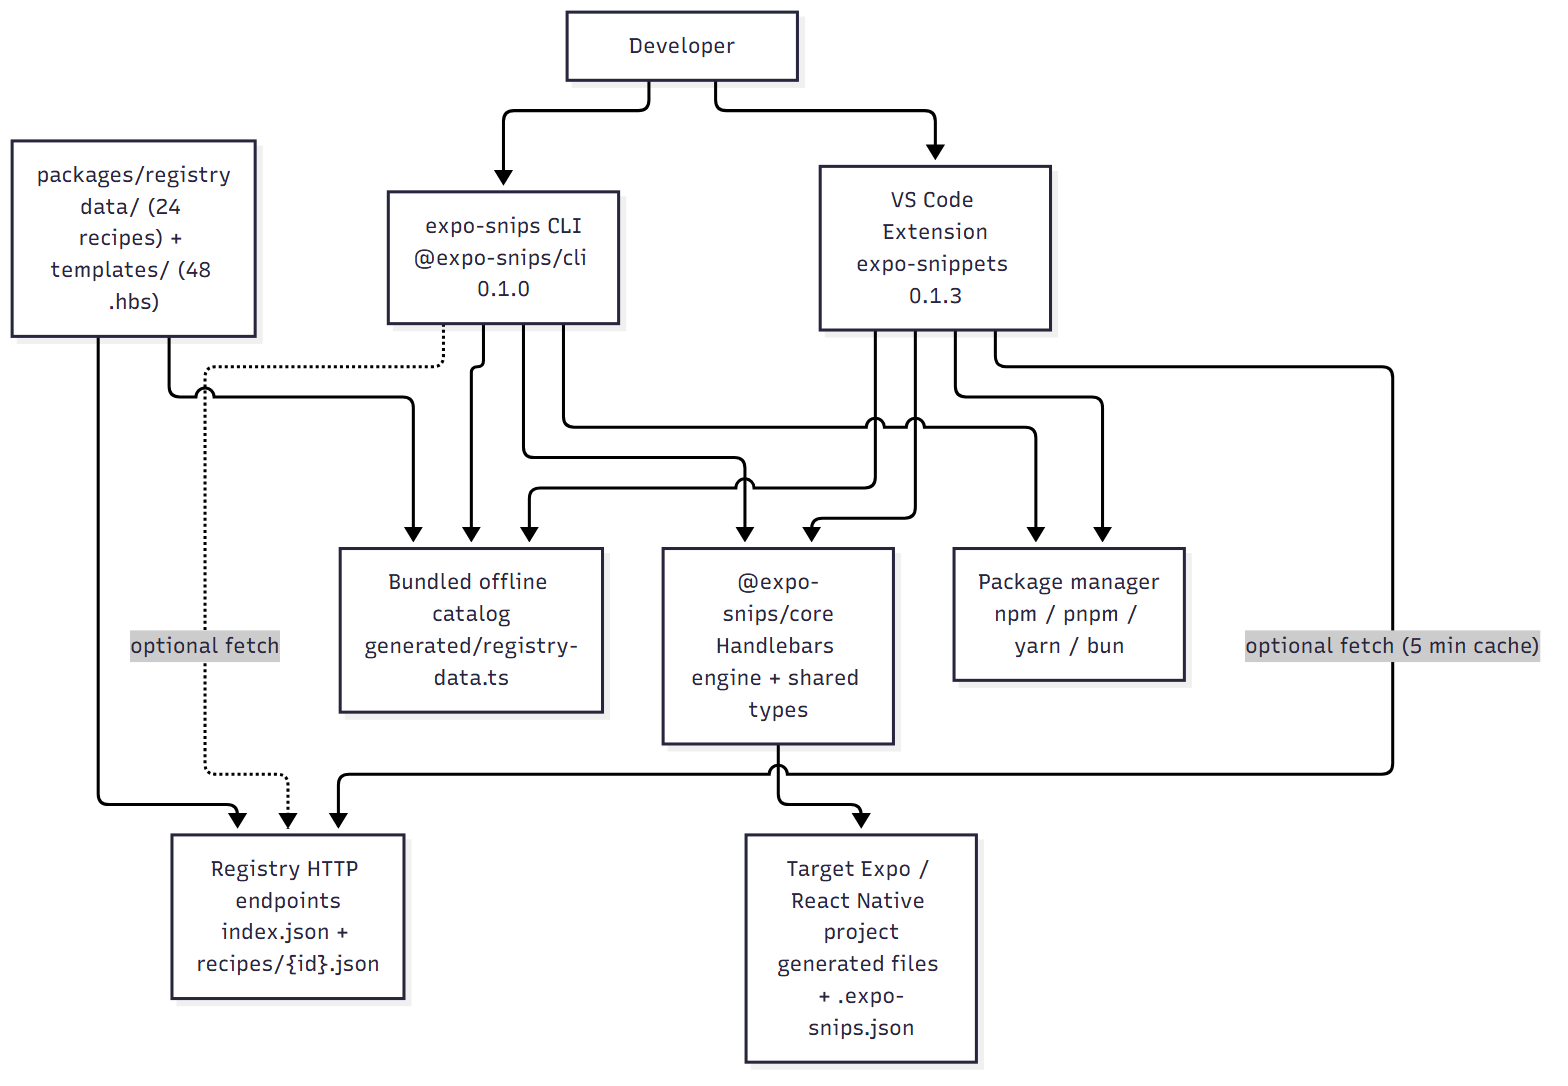
\includegraphics[width=\textwidth]{diagrams/system-architecture.png}
\caption{System architecture: clients, shared engine, catalog sources and target project}
\label{fig:system-architecture}
\end{figure}

\begin{longtable}{p{3.6cm}p{10.4cm}}
\caption{System elements}\\
\toprule
\textbf{Element} & \textbf{Responsibility and evidence} \\
\midrule

CLI client & Command parsing, interactive prompts, stack detection, orchestration and
terminal reporting. \texttt{packages/cli/src}. \\
Extension client & Command palette, completion trigger, status bar, workspace
detection, orchestration in an editor context. \texttt{packages/vscode-extension/src}. \\
Generation engine & Condition filtering and Handlebars rendering; pure functions with
no I/O. \texttt{packages/core/src}. \\
Offline catalog & Recipe arrays inlined into each client at build time
(\texttt{src/generated/registry-data.ts}, git-ignored, produced by
\texttt{scripts/prepare-registry.mjs}). \\
Registry service & Static JSON published over HTTP: \texttt{index.json} plus
per-recipe documents. \texttt{registry/}; default base
\texttt{https://registry.expo-snips.dev}. \\
Catalyst / build pipeline & Recipe source data and templates compiled into the
registry folder and into the embedded bundles.
\texttt{scripts/build-registry.mjs}, \texttt{scripts/lib/build-recipes.mjs}. \\
Target project & The user's Expo / React Native application, which receives
generated files and the \texttt{.expo-snips.json} manifest. \\
Package manager & External process used to install recipe dependencies. \\
\bottomrule
\end{longtable}

\section{Deployment topology}

\begin{itemize}
  \item \textbf{Clients} execute on the developer's machine
        (Windows, macOS or Linux).
  \item \textbf{Registry} is static hosting. The repository's own workflow deploys
        it to GitHub Pages under a \texttt{registry/} path; the code also supports
        any base URL, including a local server started with
        \texttt{pnpm serve} (default \texttt{http://localhost:3000}).
  \item \textbf{Packages} are distributed through the public npm registry.
  \item \textbf{No runtime service, message broker, cache or database exists in the
        deployed system.}
\end{itemize}

\section{Communication paths}

\begin{longtable}{p{3.2cm}p{3.4cm}p{7.4cm}}
\caption{Communication paths}\\
\toprule
\textbf{From} & \textbf{To} & \textbf{Mechanism} \\
\midrule

CLI & Registry & HTTPS GET, 10\,s abort timeout, optional; falls back to embedded catalog. \\
Extension & Registry & HTTPS GET, 10\,s abort timeout, 5-minute cache and back-off, optional. \\
CLI & Package manager & Child process (\texttt{execSync}, inherited stdio). \\
CLI & create-expo-app & Child process via \texttt{npx} (\texttt{init} only). \\
Extension & Package manager & Terminal command injection (\texttt{terminal.sendText}). \\
CLI/Extension & Target project & Local filesystem writes. \\
Clients & \texttt{@expo-snips/core} & In-process function calls (TypeScript module import). \\
Build pipeline & Registry & Local filesystem writes during CI. \\
\bottomrule
\end{longtable}

\begin{figure}[H]
\centering
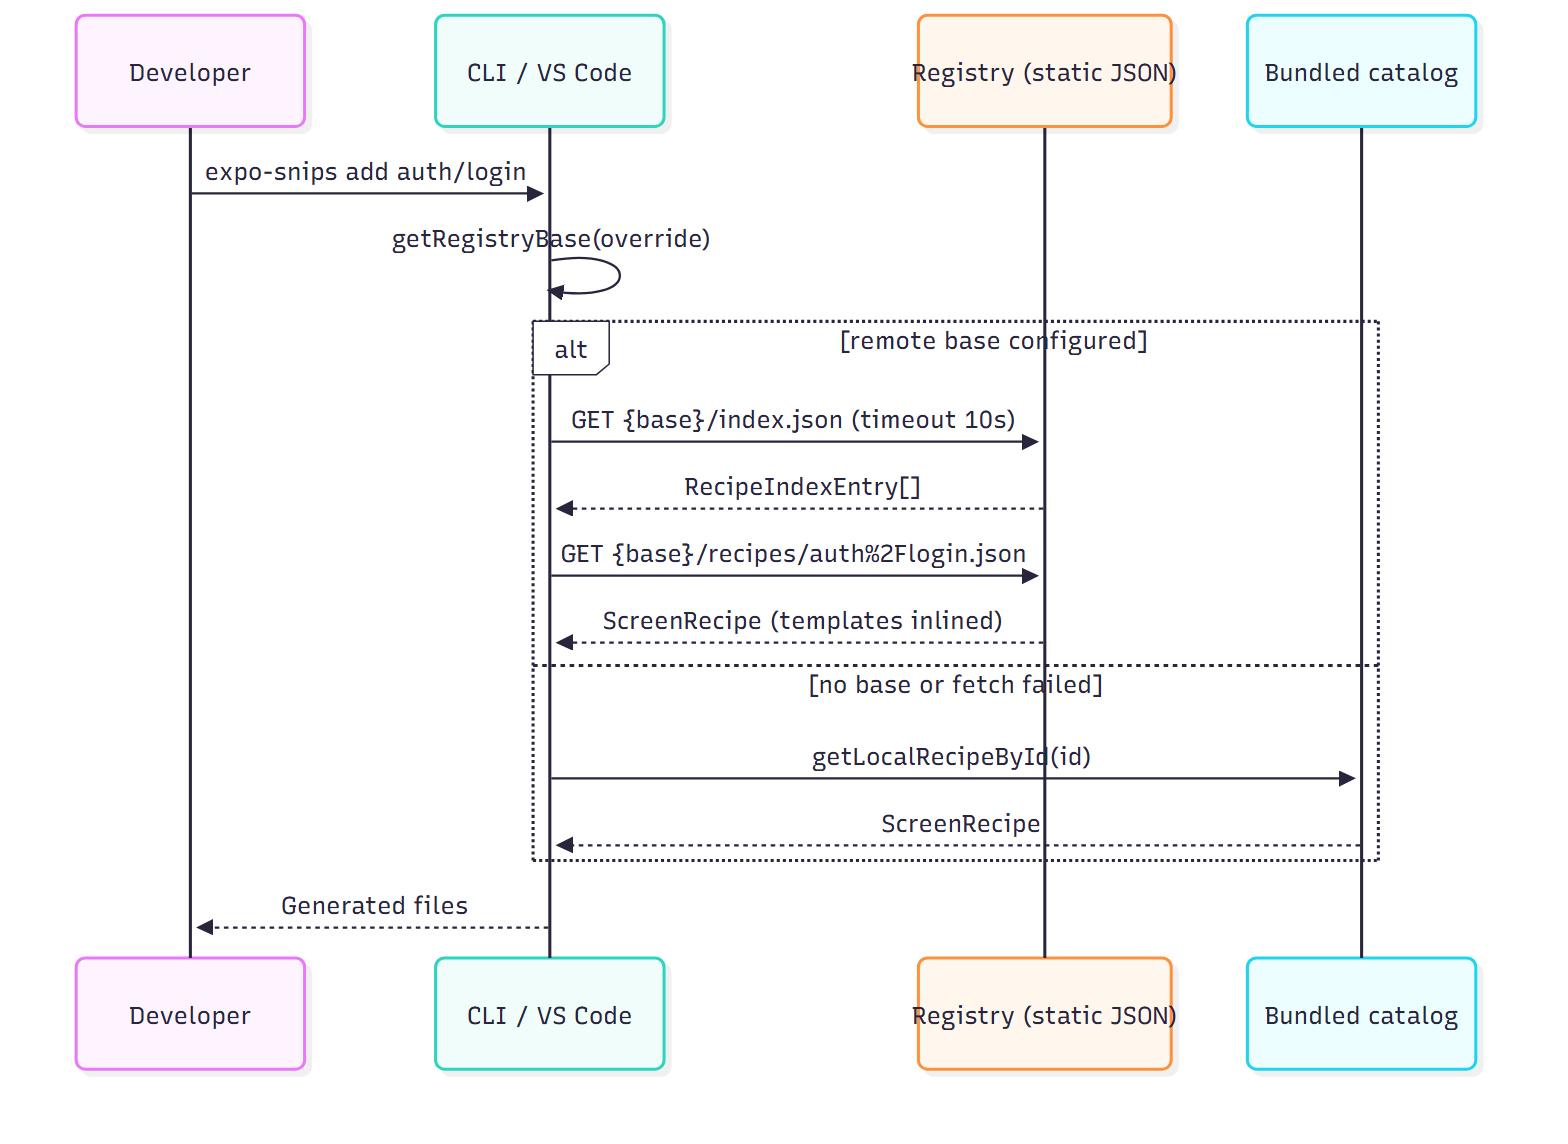
\includegraphics[width=0.92\textwidth]{diagrams/registry-api-sequence.png}
\caption{Registry resolution sequence with bundled-catalog fallback}
\label{fig:registry-api-sequence}
\end{figure}

\section{Architectural characteristics}

\begin{longtable}{p{4cm}p{10cm}}
\caption{Architectural characteristics}\\
\toprule
\textbf{Characteristic} & \textbf{Assessment} \\
\midrule

Distribution style & Local-first, offline-capable. \\
State & Stateless process; persistence only in the user's project manifest. \\
Coupling & Low-to-moderate: clients depend on the engine and on the recipe schema;
the engine has no dependency on either client. \\
Cohesion & High within each package; the recipe format is the stable contract. \\
Scalability & The catalog scales by adding files; there is no runtime scaling concern
because there is no server. \\
Failure isolation & Catalog fetch failure is contained; a failed install aborts the
CLI command after files have been written. \\
Trust boundary & The registry is trusted without verification --- the principal
architectural risk (see Chapter~\ref{ch:security}). \\
\bottomrule
\end{longtable}

\section{Key architectural decisions}

\begin{longtable}{p{1.3cm}p{5.4cm}p{7.3cm}}
\caption{Architectural decisions and rationale}\\
\toprule
\textbf{ID} & \textbf{Decision} & \textbf{Rationale / consequence} \\
\midrule

AD-01 & Inline templates into recipe JSON at build time & Consumers never need
filesystem access to templates; enables both HTTP delivery and embedded bundles.
Evidenced by \texttt{build-recipes.mjs} and the emitted recipe files. \\
AD-02 & Share one engine across clients & Guarantees identical output from CLI and
editor. Both import \texttt{getFilesForRecipe}. \\
AD-03 & Bundle the catalog in clients as well as hosting it & Guarantees offline
operation; remote registry becomes an enhancement rather than a dependency. \\
AD-04 & Recipes are data, not code & New screens need no engine change; validated by
schema. Trade-off: template strings are embedded in JSON, which is awkward to edit
and diff but trivially portable. \\
AD-05 & Use Handlebars rather than a stronger typed generator & Minimal dependency
footprint in the engine (one runtime dependency) at the cost of limited type safety
inside templates (INFERRED). \\
AD-06 & Force \texttt{nativewind} + \texttt{lucide} when \texttt{ui=shadcn} & The
shadcn-style primitives depend on NativeWind utility classes and lucide icons;
enforced rather than validated. \\
AD-07 & Persist installs in a project-local manifest & Enables update and status
workflows without any server-side account. \\
\bottomrule
\end{longtable}

\section{Constraints and limitations of the architecture}

\begin{itemize}
  \item No plugin or extension mechanism exists inside the clients; adding a screen
        means adding catalogue data, not extending the CLI.
  \item The engine's generated output depends on the recipe's \texttt{when}
        conditions being written correctly; there is no schema check that every
        supported option combination yields at least one file for every required
        path.
  \item Because templates are inlined into JSON, template content is escaped and
        difficult to review in the built registry (see the \texttt{auth/login}
        built recipe, where multi-line templates appear as single escaped lines).
  \item The extension duplicates the CLI's detection and primitive-resolution logic
        rather than importing it, so the two can drift.
\end{itemize}

\textbf{Status:} IMPLEMENTED (the first, second and fourth items are directly
observable); INFERRED (the third).

\chapter{Software Architecture}
\label{ch:software-architecture}

\section{Package structure}

The repository is a pnpm workspace with four packages. Dependencies flow in one
direction only: every package may depend on \texttt{@expo-snips/core}; the core
depends on nothing from the workspace.

\begin{figure}[H]
\centering
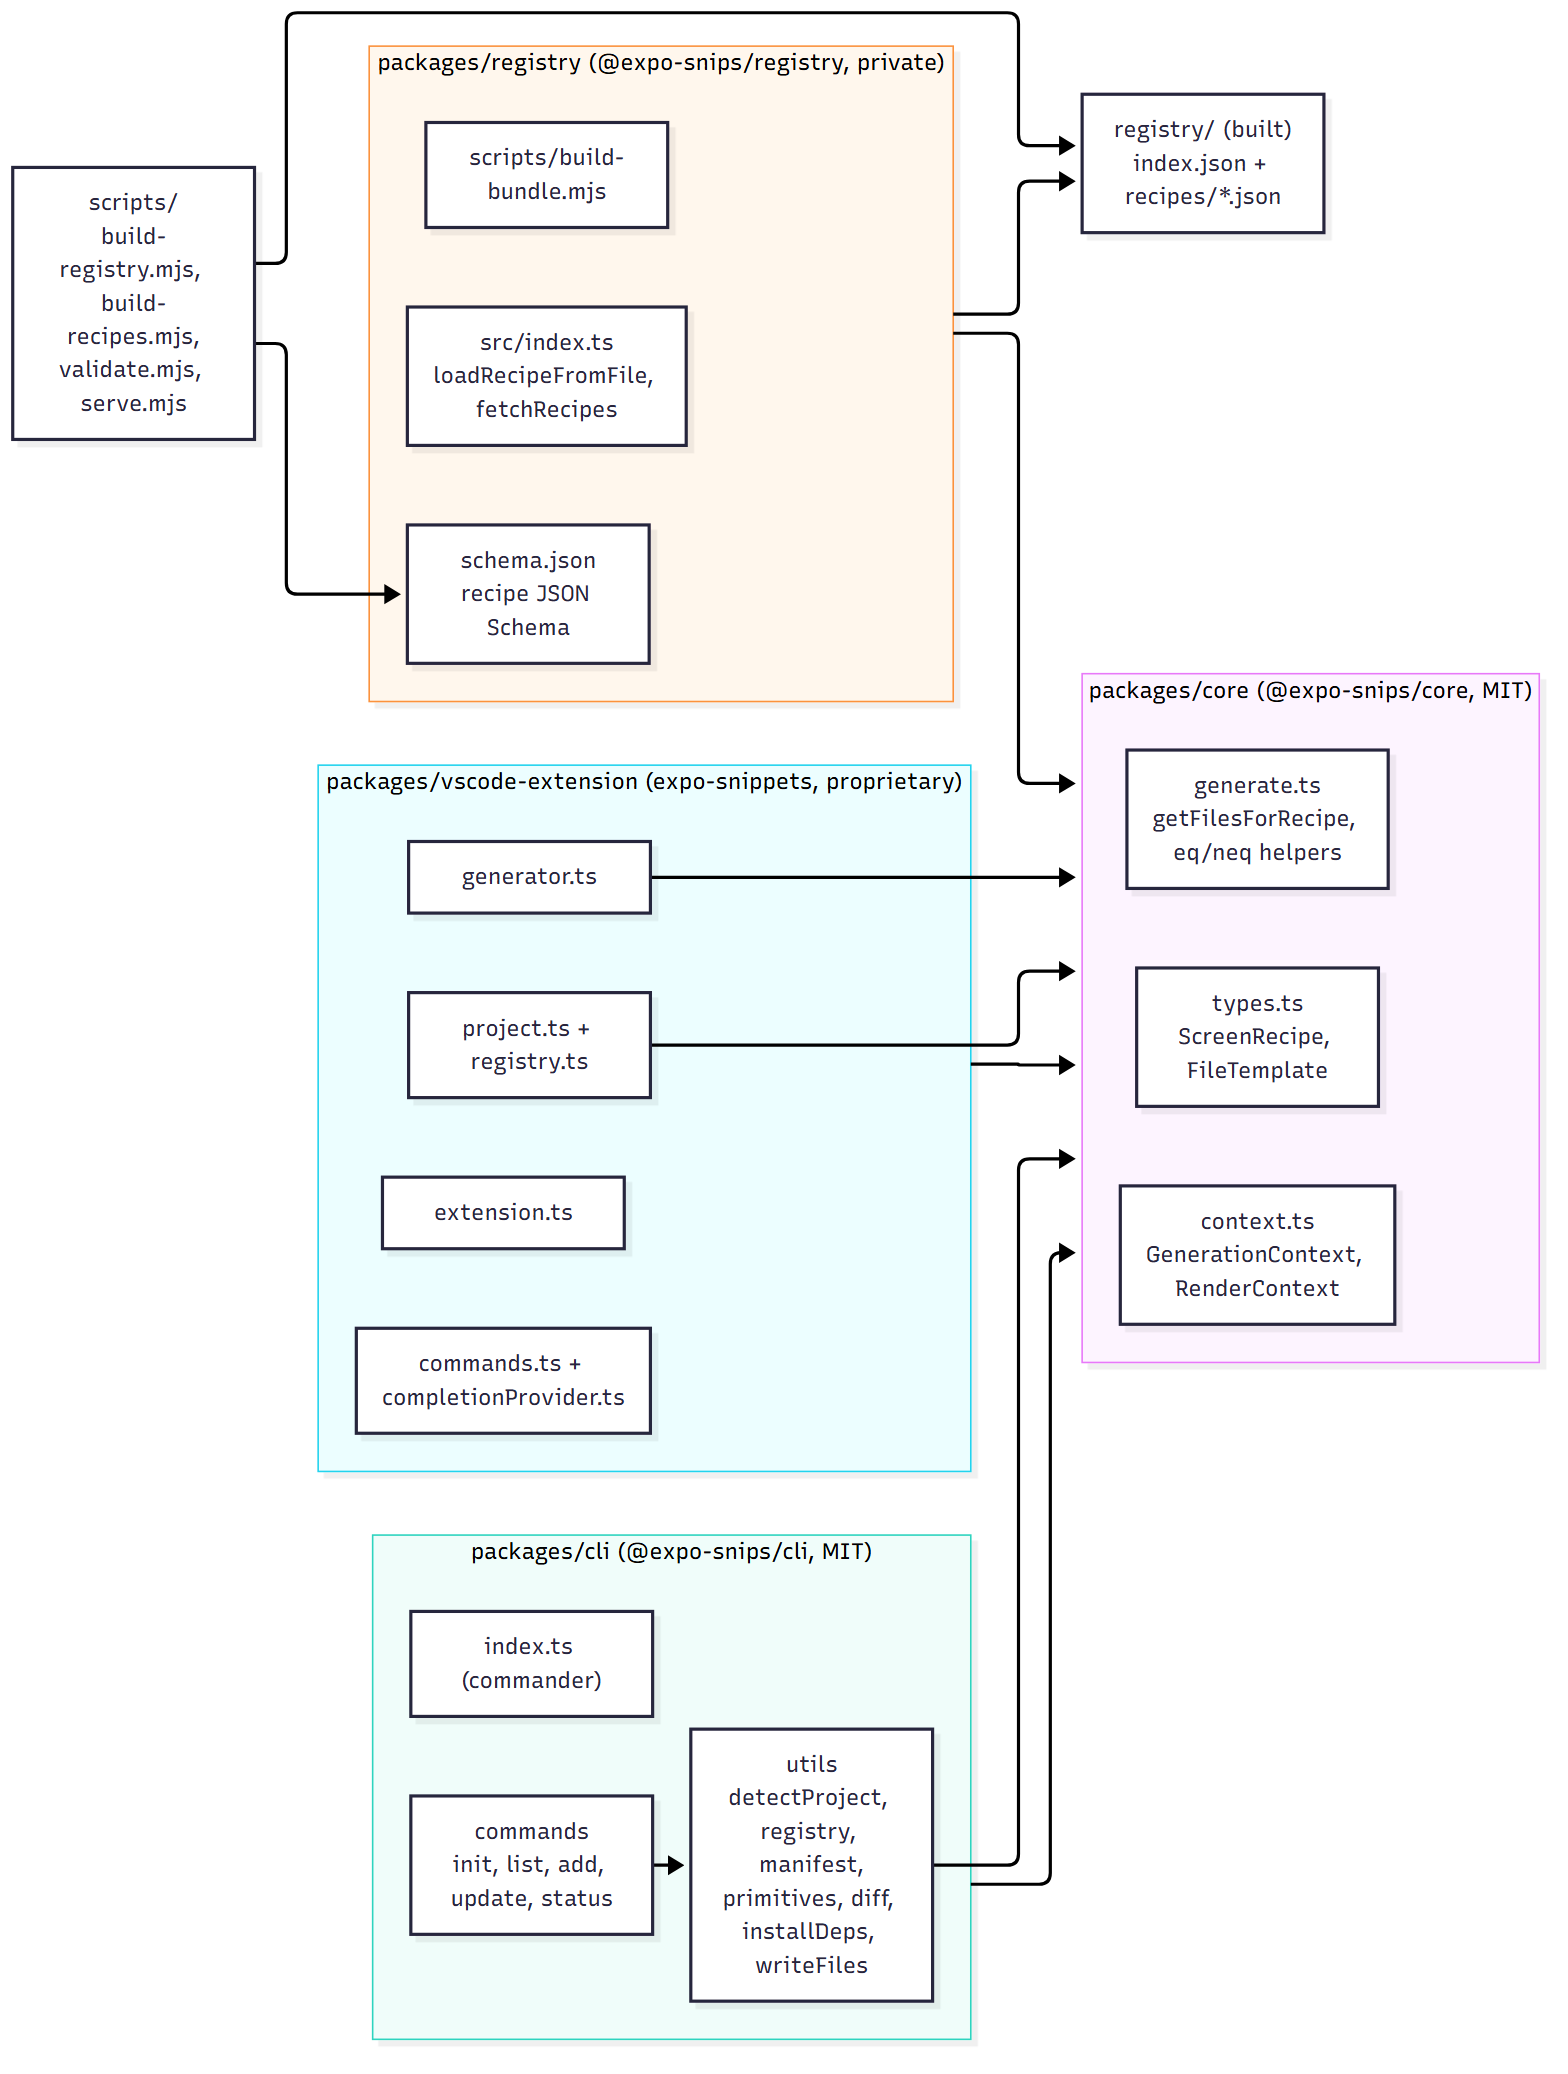
\includegraphics[width=\textwidth]{diagrams/component-architecture.png}
\caption{Component architecture of the pnpm workspace}
\label{fig:component-architecture}
\end{figure}

\begin{longtable}{p{3.6cm}p{2.6cm}p{1.9cm}p{5.9cm}}
\caption{Package inventory}\\
\toprule
\textbf{Package} & \textbf{Name} & \textbf{Visibility} & \textbf{Responsibility} \\
\midrule

\texttt{packages/core} & \texttt{@expo-snips/core} & public (MIT) & Shared types, generation context and the Handlebars rendering engine. \\
\texttt{packages/cli} & \texttt{@expo-snips/cli} & public (MIT) & Terminal client: commands, detection, orchestration, manifest, diff. \\
\texttt{packages/registry} & \texttt{@expo-snips/registry} & private & Recipe data (24), templates (48), JSON Schema, bundle builder, filesystem + HTTP loaders. \\
\texttt{packages/vscode-extension} & \texttt{expo-snippets} & proprietary & VS Code client: commands, completion, status bar, workspace detection, generation. \\
\bottomrule
\end{longtable}

Workspace dependency declarations:
\texttt{"@expo-snips/core": "workspace:*"} in \texttt{packages/cli/package.json} and
\texttt{packages/registry/package.json}; a development dependency on
\texttt{@expo-snips/core} in \texttt{packages/vscode-extension/package.json}
(the engine is bundled into the extension by esbuild).

\section{Module boundaries}

\subsection*{\texttt{@expo-snips/core}}

\begin{longtable}{p{2.8cm}p{11.2cm}}
\toprule
\textbf{Module} & \textbf{Contents} \\
\midrule
\endhead
\texttt{types.ts} & \texttt{StylingOption}, \texttt{RouterOption}, \texttt{UIOption},
\texttt{IconOption}, \texttt{Conditions}, \texttt{FileTemplate} (with
\texttt{perStyling} and \texttt{variants} override maps), \texttt{ScreenVariant},
\texttt{ScreenRecipe}. \\
\texttt{context.ts} & \texttt{GenerationOptions}, \texttt{GenerationContext}
(project root, options, optional variant), \texttt{RenderContext}. \\
\texttt{generate.ts} & Registers the \texttt{eq}/\texttt{neq} Handlebars helpers;
exposes \texttt{renderTemplate}, \texttt{getFilesForRecipe}; privately
\texttt{resolveTemplateString} (variant $\rightarrow$ per-styling $\rightarrow$
template precedence) and \texttt{matchesCondition}. \\
\texttt{index.ts} & Barrel re-export of the three modules above. \\
\bottomrule
\end{longtable}

The core performs no I/O and has no knowledge of the CLI, the extension or the
filesystem. This makes it the natural unit-test target, although no tests exist.

\subsection*{\texttt{@expo-snips/cli}}

\begin{longtable}{p{4.2cm}p{9.8cm}}
\toprule
\textbf{Module} & \textbf{Contents} \\
\midrule
\endhead
\texttt{index.ts} & Creates the \texttt{Command} program, sets name/description/version, registers the five subcommands. \\
\texttt{commands/init.ts} & Project bootstrap via \texttt{create-expo-app}; refuses when \texttt{app.json} exists. \\
\texttt{commands/list.ts} & Prints the resolved catalog with source attribution. \\
\texttt{commands/add.ts} & The main generation command: registry resolution, detection, option resolution, prompts, rendering, writing, primitives, install, manifest. \\
\texttt{commands/status.ts} & Prints manifest entries. \\
\texttt{commands/update.ts} & Re-renders tracked screens, diffs, confirms, writes, bumps versions. \\
\texttt{utils/detectProject.ts} & \texttt{detectProject(dir)} --- reads \texttt{package.json} and \texttt{tsconfig.json}. \\
\texttt{utils/registry.ts} & Registry base resolution, remote fetch with timeout, embedded-catalog fallback. \\
\texttt{utils/resolveRegistry.ts} & Wraps index resolution with user-facing source reporting. \\
\texttt{utils/manifest.ts} & Manifest read/write/upsert/version-bump. \\
\texttt{utils/primitives.ts} & Recursive primitive resolution. \\
\texttt{utils/installDeps.ts} & Package-manager detection and dependency installation. \\
\texttt{utils/writeFiles.ts} & Directory creation and file writing with per-file logging. \\
\texttt{utils/diff.ts} & LCS line diff and coloured printing. \\
\texttt{generated/registry-data.ts} & Build-time generated embedded catalog (git-ignored). \\
\bottomrule
\end{longtable}

\subsection*{\texttt{@expo-snips/registry}}

\begin{itemize}
  \item \texttt{src/index.ts} --- \texttt{loadRecipeFromFile} (inlines
        \texttt{templateFile}, variant and per-styling references),
        \texttt{getAllRecipes}, \texttt{getRecipeById}, \texttt{searchRecipes} and
        \texttt{fetchRecipes} (accepts an array, a \texttt{\{recipes\}} bundle or a
        single recipe object).
  \item \texttt{schema.json} --- the recipe JSON Schema used by the validator.
  \item \texttt{data/**} --- 24 recipe source files organised by category.
  \item \texttt{templates/**} --- 48 Handlebars templates organised by category.
  \item \texttt{scripts/build-bundle.mjs} --- writes \texttt{bundle.json} (a
        \texttt{\{version, name, recipes\}} bundle, 24 recipes).
\end{itemize}

\subsection*{\texttt{expo-snippets} (VS Code extension)}

\begin{longtable}{p{4.2cm}p{9.8cm}}
\toprule
\textbf{Module} & \textbf{Contents} \\
\midrule
\endhead
\texttt{extension.ts} & \texttt{activate()}: registers commands and completion
provider, creates the status bar item; \texttt{deactivate()} is empty. \\
\texttt{commands.ts} & \texttt{expo-snips.addScreen} (Quick Pick) and
\texttt{expo-snips.generateFromCompletion}. \\
\texttt{completionProvider.ts} & Completion provider for the four TS/JS language
ids, triggered on \texttt{:}, matching \texttt{snip:} / \texttt{expo-snips:}. \\
\texttt{generator.ts} & \texttt{resolveOptions}, \texttt{pickVariant},
\texttt{detectPackageManager}, \texttt{installDependencies},
\texttt{resolvePrimitives}/\texttt{getPrimitives} and \texttt{generateScreen}. \\
\texttt{project.ts} & \texttt{getWorkspaceRoot}, \texttt{detectProject} and the
manifest functions. \\
\texttt{registry.ts} & Embedded catalog, remote index/recipe fetch, 5-minute cache
and back-off. \\
\bottomrule
\end{longtable}

\section{Dependency graph}

\begin{table}[H]
\centering
\caption{Runtime and build dependencies}
\begin{longtable}{p{3.6cm}p{4.6cm}p{5.8cm}}
\toprule
\textbf{Package} & \textbf{Runtime dependencies} & \textbf{Dev / build dependencies} \\
\midrule
\endhead
core & handlebars \^{}4.7.8 & typescript \^{}5.5 \\
cli & @expo-snips/core (workspace), chalk \^{}4.1.2, commander \^{}12, fs-extra \^{}11.2, prompts \^{}2.4.2 & @types/fs-extra, @types/node \^{}20, @types/prompts, typescript \^{}5.5 \\
registry & @expo-snips/core (workspace) & @types/node \^{}20, typescript \^{}5.5 \\
vscode-extension & (none at runtime; engine bundled) & @expo-snips/core, @types/fs-extra, @types/node \^{}20, @types/vscode \^{}1.80, @vscode/vsce \^{}2.24, esbuild \^{}0.21.5, fs-extra \^{}11.2, typescript \^{}5.5 \\
\bottomrule
\end{longtable}
\end{table}

\section{Build pipeline}

\begin{longtable}{p{4cm}p{10cm}}
\toprule
\textbf{Package} & \textbf{Build command and behaviour} \\
\midrule
\endhead
core & \texttt{tsc -p tsconfig.json} --- emits \texttt{dist/} with declarations and source maps. \\
cli & \texttt{node scripts/prepare-registry.mjs \&\& tsc -p tsconfig.json} --- regenerates the embedded catalog, then compiles. \\
registry & \texttt{tsc} (library build) and \texttt{node scripts/build-bundle.mjs} (\texttt{build:bundle}). \\
vscode-extension & \texttt{node esbuild.mjs} --- runs \texttt{prepareRegistry()} first, then bundles to \texttt{out/extension.js}. \\
root & \texttt{pnpm -r build}; also \texttt{validate}, \texttt{build:registry} and \texttt{serve} scripts. \\
\bottomrule
\end{longtable}

\section{Code-size profile}

The hand-written TypeScript across the workspace (excluding type declarations and
generated catalog modules) is approximately 1{,}600 lines. The largest single
source files are \texttt{generator.ts} (268 lines), \texttt{add.ts} (279 lines) and
\texttt{update.ts} (150 lines). No file is pathological in size; the largest
codebase element by far is the recipe data and template set (24 recipes and 48
templates).

\textbf{Status:} IMPLEMENTED (measured) / INFERRED (assessment that no file is
pathological).

\chapter{High-Level Design}
\label{ch:high-level-design}

\section{Design intent}

The high-level design separates four concerns:

\begin{enumerate}
  \item \textbf{Catalog} --- what screens exist and what they need (data only).
  \item \textbf{Engine} --- how a recipe becomes files (pure transformation).
  \item \textbf{Clients} --- how a developer reaches the engine (I/O and UX).
  \item \textbf{Delivery} --- how catalog and packages reach the developer (build
        and CI).
\end{enumerate}

This separation is what allows the same recipe to be rendered by a terminal
program and by an editor extension with identical results.

\section{End-to-end generation flow}

\begin{figure}[H]
\centering
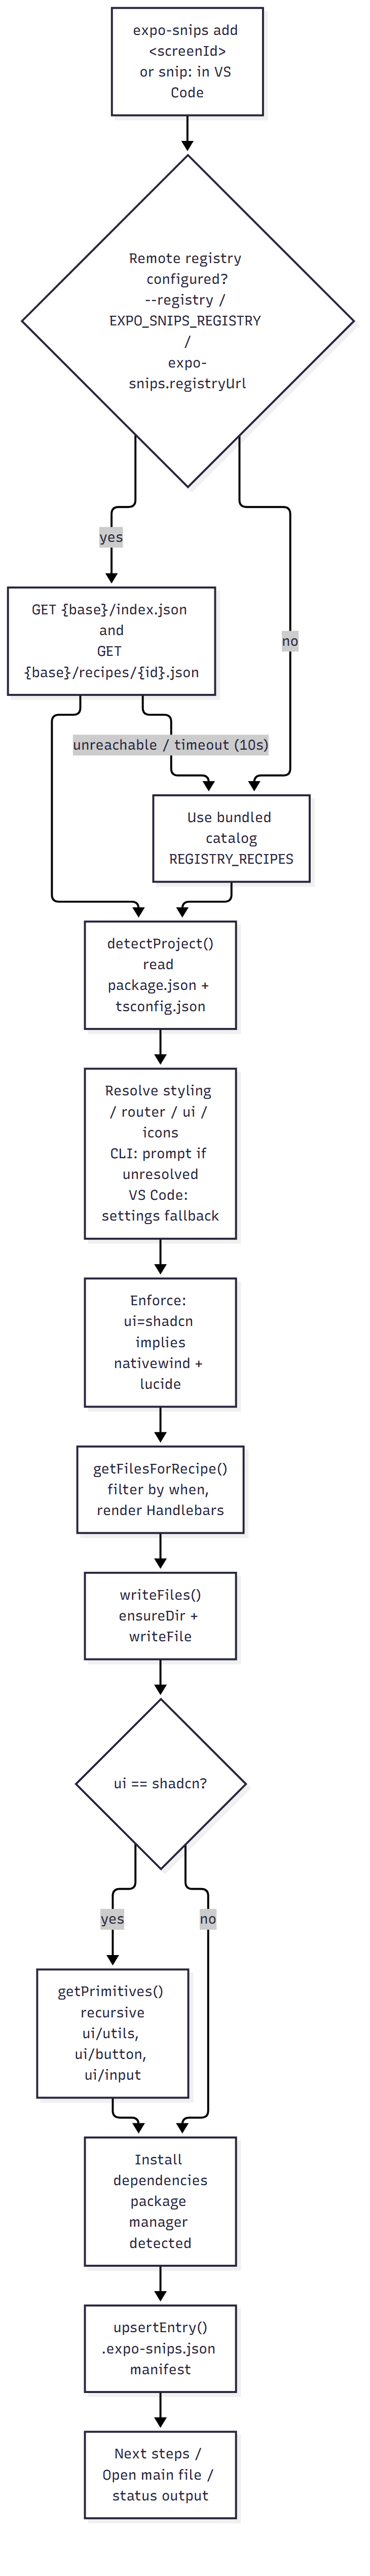
\includegraphics[width=\textwidth]{diagrams/generation-pipeline.png}
\caption{High-level generation pipeline from command to persisted manifest}
\label{fig:generation-pipeline}
\end{figure}

The pipeline has seven stages, each implemented in a single, identifiable place:

\begin{longtable}{p{1cm}p{3.8cm}p{9.2cm}}
\caption{Pipeline stages}\\
\toprule
\textbf{\#} & \textbf{Stage} & \textbf{Implementation} \\
\midrule

1 & Resolve input & Parse the screen id and flags; fetch or select the recipe
(\texttt{add.ts}, \texttt{registry.ts}). \\
2 & Detect environment & Read \texttt{package.json} / \texttt{tsconfig.json}
(\texttt{detectProject.ts}). \\
3 & Resolve options & Apply precedence rules and prompts; enforce shadcn
constraints (\texttt{add.ts}). \\
4 & Render & Filter file entries by \texttt{when}; select template; compile with
Handlebars (\texttt{core/src/generate.ts}). \\
5 & Persist files & Create directories and write content
(\texttt{writeFiles.ts}). \\
6 & Resolve primitives & Recursively emit shadcn primitives, skipping existing
files (\texttt{primitives.ts}). \\
7 & Finalise & Install dependencies and record the install
(\texttt{installDeps.ts}, \texttt{manifest.ts}). \\
\bottomrule
\end{longtable}

\section{Major services and how they communicate}

There are no long-running services. The system's ``services'' are libraries and
one static endpoint.

\begin{longtable}{p{3.8cm}p{4.6cm}p{5.6cm}}
\caption{Service-equivalent components and their interactions}\\
\toprule
\textbf{Component} & \textbf{Interaction style} & \textbf{Peer} \\
\midrule

Generation engine & In-process function calls & CLI client, extension client \\
Embedded catalog & In-memory module import & CLI client, extension client \\
Registry endpoint & HTTP GET, JSON, read-only & Both clients (optional) \\
Package manager & Child process / terminal text & CLI client, extension client \\
create-expo-app & Child process & CLI client \\
VS Code host & Extension API & Extension client \\
\bottomrule
\end{longtable}

\section{Data model at a high level}

\begin{itemize}
  \item \textbf{Recipe} --- identity, version, supported stacks, dependencies,
        file templates (with conditions and overrides), optional variants, tags and
        primitive references. Defined by \texttt{ScreenRecipe} in
        \texttt{core/src/types.ts} and constrained by \texttt{registry/schema.json}.
  \item \textbf{Catalog index entry} --- the recipe subset needed for browsing:
        id, name, description, version, typescript flag, tags, supported stacks.
  \item \textbf{Generated file} --- a path plus rendered content.
  \item \textbf{Manifest entry} --- the record that a recipe was installed into a
        project.
\end{itemize}

\section{Cross-cutting concerns}

\begin{longtable}{p{3.6cm}p{10.4cm}}
\caption{Cross-cutting concerns and their handling}\\
\toprule
\textbf{Concern} & \textbf{Handling} \\
\midrule

Error reporting & Coloured console output (CLI); VS Code error/information messages (extension). Non-zero exit code on failure. \\
Configuration & CLI flags and \texttt{EXPO\_SNIPS\_REGISTRY}; six VS Code settings. No config files. \\
Logging & Untyped console output; no log levels or destinations. \\
Offline behaviour & Embedded catalog; graceful fallback on every network failure. \\
Versioning & Semver on recipes and packages; the manifest stores the installed recipe version. \\
Extensibility & New recipes and new templates require no code change; new options would require type, schema, CLI-choice and settings changes. \\
\bottomrule
\end{longtable}

\section{Design trade-offs}

\begin{longtable}{p{4.6cm}p{4.4cm}p{5cm}}
\caption{Principal design trade-offs}\\
\toprule
\textbf{Choice} & \textbf{Benefit} & \textbf{Cost} \\
\midrule

Templates in JSON (inlined) & Portable, dependency-free rendering; works offline and over HTTP. & Poor diffs and review ergonomics in the built registry; JSON escaping of large templates. \\
Handlebars & One dependency; familiar syntax; easy recipe authoring. & Unchecked at compile time; typos surface only at render time. \\
Option enforcement instead of validation & Simpler command code. & Silent reprioritisation of user choices when \texttt{ui=shadcn} is selected. \\
Unconditional file writes on \texttt{add} & Simple, predictable generation. & A pre-existing file at a recipe path is overwritten with no warning. \\
Duplicated detection logic in the extension & Avoids a shared dependency on CLI internals. & Two implementations can diverge. \\
\bottomrule
\end{longtable}

\chapter{Low-Level Design}
\label{ch:low-level-design}

This chapter documents the significant functions, their signatures, their inputs
and outputs, and the state they touch. Signatures are reproduced from the source.

\section{\texttt{@expo-snips/core}}

\subsection*{\texttt{renderTemplate(templateStr, context)}}

\begin{lstlisting}[language=JavaScript]
export function renderTemplate(templateStr: string, context: RenderContext): string
\end{lstlisting}

Compiles the template with Handlebars and executes it against the render context.
Compilation happens per call; there is no cache.

\subsection*{\texttt{getFilesForRecipe(recipe, context, resolveFile?)}}

\begin{lstlisting}[language=JavaScript]
export function getFilesForRecipe(
  recipe: ScreenRecipe,
  context: GenerationContext,
  resolveFile?: (file: FileTemplate) => string | null
): Array<{ path: string; content: string }>
\end{lstlisting}

Algorithm:

\begin{enumerate}
  \item For each entry in \texttt{recipe.files}, evaluate \texttt{when} via
        \texttt{matchesCondition}; skip on mismatch.
  \item Resolve the template string with \texttt{resolveTemplateString}: variant
        override, then per-styling override, then \texttt{template}.
  \item If the template is still null and \texttt{templateFile} is set, delegate to
        the optional \texttt{resolveFile} callback (used when templates were not
        inlined).
  \item Skip the entry if no template could be resolved.
  \item Render and append \texttt{\{path, content\}}.
\end{enumerate}

Only \texttt{path} and \texttt{content} are returned; conditions and metadata are
discarded. Consequently two file entries targeting the same path (a common recipe
pattern --- one entry per supported stack) are filtered down to the single entry
whose conditions match.

\subsection*{\texttt{matchesCondition} (private)}

Evaluates five optional predicates in sequence --- styling, router, ui, icons and
typescript --- returning false on the first mismatch. TypeScript comparison is an
exact equality check, so \texttt{typescript: false} matches only JavaScript
generation.

\subsection*{\texttt{buildRenderContext} (private)}

Projects the generation context into the render context by duplicating the option
values at the top level (\texttt{styling}, \texttt{router}, \texttt{ui},
\texttt{icons}, \texttt{typescript}) so templates can be written as
\texttt{\{\#if (eq styling "nativewind")\}} without an options prefix.

\section{\texttt{@expo-snips/cli} --- utilities}

\begin{longtable}{p{4.2cm}p{9.8cm}}
\caption{CLI utility functions}\\
\toprule
\textbf{Function} & \textbf{Behaviour} \\
\midrule

\texttt{detectProject(dir?)} & Reads \texttt{package.json} for four dependency
probes and \texttt{tsconfig.json} for the language flag; returns
\texttt{DetectedProject}. Defaults: ui \texttt{native}, icons \texttt{none},
styling \texttt{stylesheet} when no \texttt{package.json} exists. \\
\texttt{getRegistryBase(override?)} & Returns \texttt{(override || env || "").trim()}
with trailing slashes removed. \\
\texttt{hasLocalRegistry()} & True when the embedded catalog is non-empty. \\
\texttt{getLocalRecipeById(id)} & Map lookup into the embedded catalog. \\
\texttt{fetchJSON<T>(url)} & \texttt{fetch} with a 10-second \texttt{AbortController}
timeout; returns null on non-OK responses. \\
\texttt{resolveRecipeIndex(base?)} & Remote fetch first; falls back to the local
index; reports \texttt{source} as \texttt{"remote"} or \texttt{"local"}. \\
\texttt{getRecipeIndex(base?)} & Index only. \\
\texttt{getRecipeById(id, base?)} & Remote recipe fetch, then embedded lookup. \\
\texttt{getRecipesByIds(ids, base?)} & Parallel resolve, filtering nulls. \\
\texttt{resolveRegistry(url?)} & Calls \texttt{resolveRecipeIndex} and prints a
source message. \\
\texttt{readManifest(dir?)} & Returns \texttt{\{version:1, installs:[]\}} when the file
is absent or unparseable. \\
\texttt{upsertEntry(entry, dir?)} & Replaces the entry matching
(\texttt{recipeId}, \texttt{variant}) or appends. \\
\texttt{updateEntryVersions(entries, dir?)} & Rewrites \texttt{recipeVersion} for
matching entries. \\
\texttt{getPrimitives(recipe, context, root, findRecipe)} & Recursive primitive
resolution with a \texttt{Set} cycle guard; dedupes dependencies. \\
\texttt{installDependencies(deps, devDeps, dir?)} & Detects the package manager and
runs \texttt{add} / \texttt{add -D}. \\
\texttt{writeFiles(files, root)} & \texttt{ensureDir} then \texttt{writeFile} per
file, logging each path. \\
\texttt{diffLines(oldText, newText)} & Builds an $(n+1)\times(m+1)$ LCS table and
walks it to emit add/remove/context hunks. \\
\texttt{printDiff(path, old, new)} & Prints coloured hunks; no output when nothing
changed. \\
\texttt{hasChanges(old, new)} & Strict string inequality. \\
\bottomrule
\end{longtable}

\subsection*{Manifest data structures}

\begin{lstlisting}[language=JavaScript]
interface ManifestOptions { styling: string; router: string; ui: string; icons: string; typescript: boolean; }
interface ManifestEntry { recipeId: string; recipeVersion: string; installedAt: string; options: ManifestOptions; variant?: string; files: string[]; }
interface Manifest { version: number; installs: ManifestEntry[]; }
const MANIFEST_FILENAME = ".expo-snips.json";
\end{lstlisting}

\subsection*{The \texttt{add} command in detail}

\texttt{add.ts} is the longest command and the best illustration of the CLI's
control flow.

\begin{longtable}{p{1.5cm}p{12.3cm}}
\caption{\texttt{add} command steps}\\
\toprule
\textbf{Lines} & \textbf{Step} \\
\midrule

68--70 & Resolve the registry; prepare a \texttt{findRecipe} closure. \\
72--92 & If no id was supplied, list the index in a select prompt; abort with exit
code 1 if empty or cancelled. \\
94--100 & Load the recipe; error with guidance if not found. \\
102 & Detect the project. \\
104--117 & Resolve styling; validate any explicit value; fall back to a detected
value only when the recipe supports it. \\
119--159 & Resolve router, ui and icons with the same pattern, including the
``single supported value'' shortcut. \\
161--165 & Resolve language; warn when a TypeScript recipe is generated as
JavaScript. \\
167--200 & Prompt for any option still unresolved, offering only supported values
and preselecting the detected one. \\
202--214 & Enforce the shadcn constraints. \\
216--222 & Build the generation context with \texttt{projectRoot: process.cwd()}. \\
224--230 & Render; error when no files matched. \\
232--238 & Announce the recipe and the effective option values. \\
238 & Write files. \\
240--256 & Resolve and write shadcn primitives; merge their dependencies; report
skipped files. \\
258--260 & Install dependencies unless \texttt{--no-install} was given. \\
262--272 & Upsert the manifest entry. \\
274--278 & Print success and next steps. \\
\bottomrule
\end{longtable}

\textbf{Observation.} Styling resolution appears twice: lines 111--117 compute a
detected styling, and lines 167--173 recompute the same value before prompting.
The duplicate is harmless but redundant (recorded in
Chapter~\ref{ch:technical-debt}).

\section{The recipe primitive graph}

\begin{figure}[H]
\centering
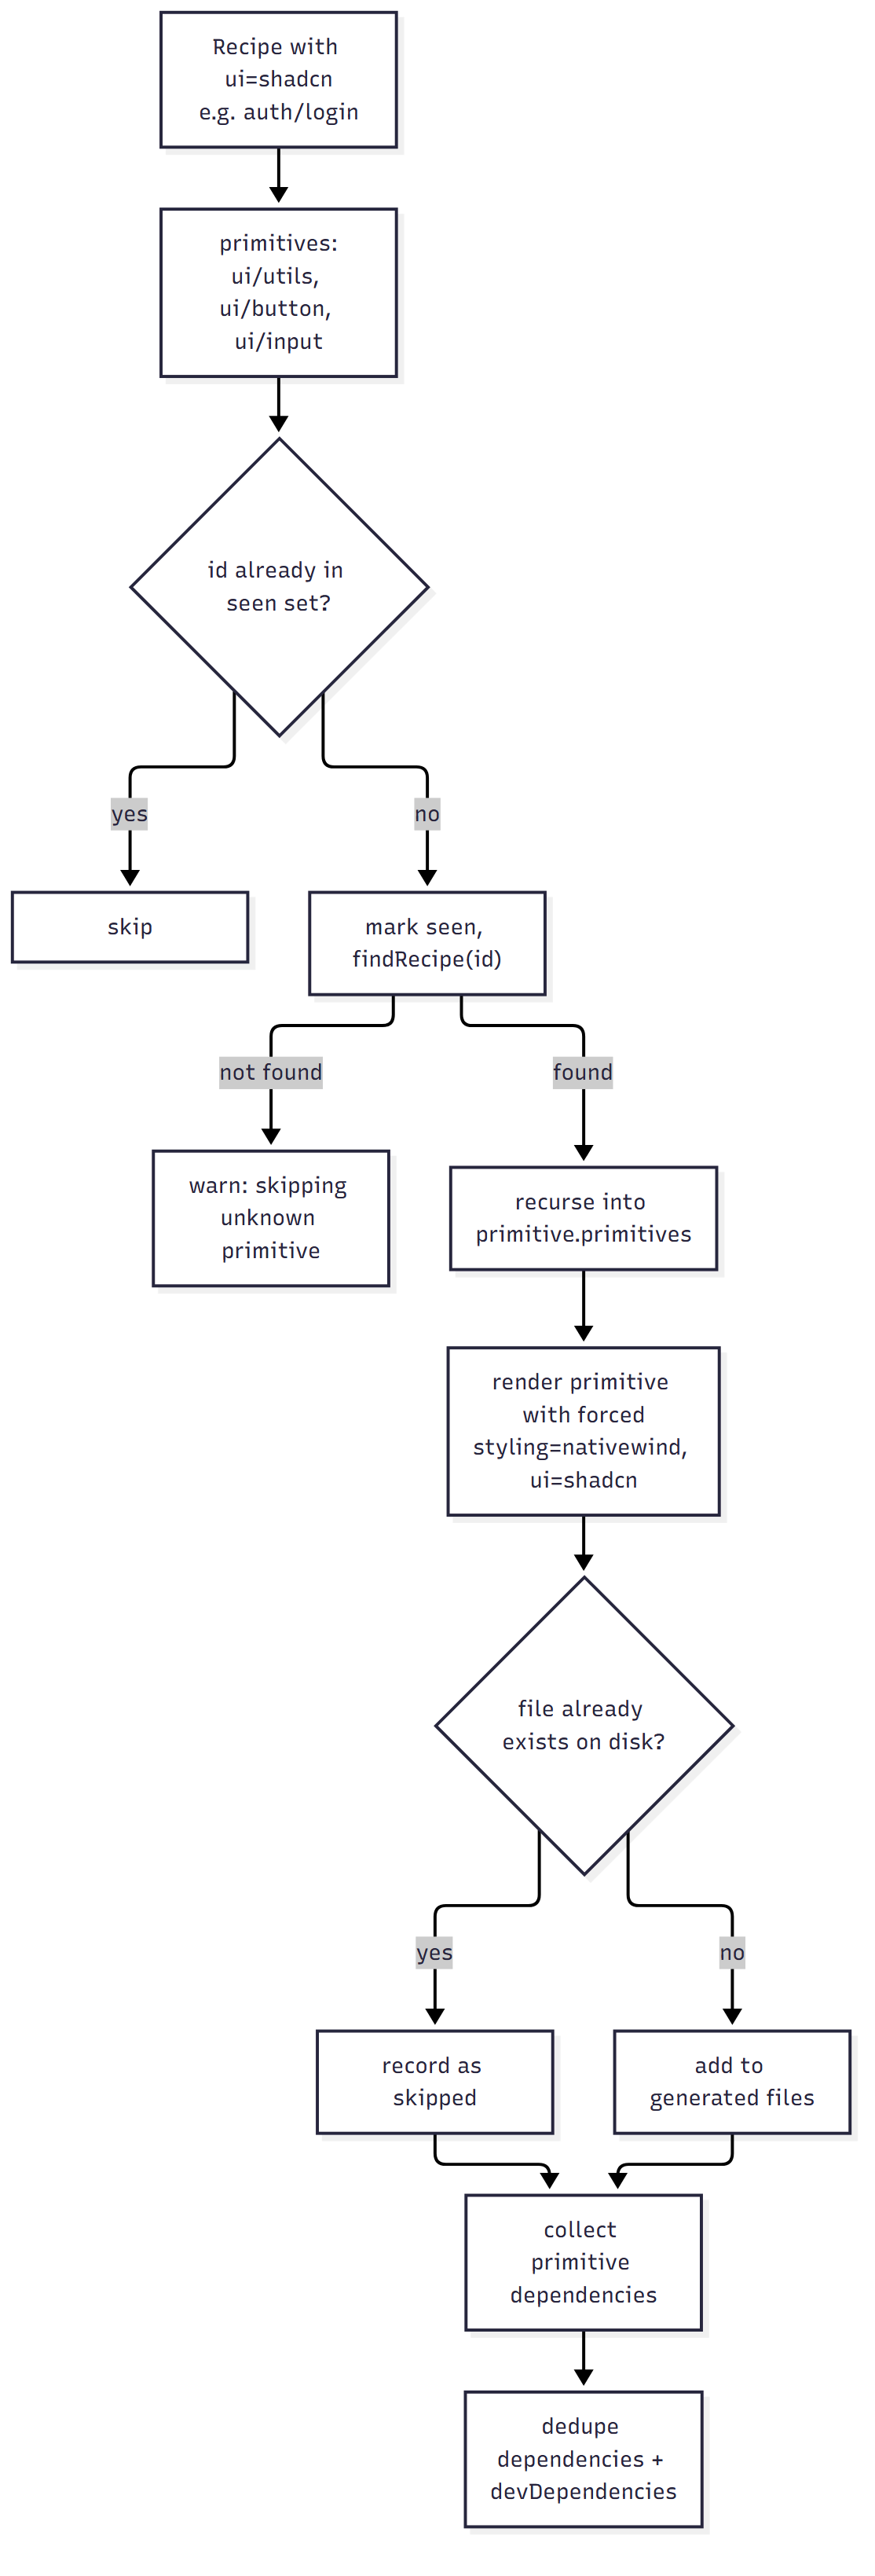
\includegraphics[width=0.95\textwidth]{diagrams/primitive-resolution.png}
\caption{Recursive UI primitive resolution when \texttt{ui=shadcn}}
\label{fig:primitive-resolution}
\end{figure}

\section{\texttt{expo-snippets} --- VS Code extension}

\begin{longtable}{p{4.2cm}p{9.8cm}}
\caption{Extension functions}\\
\toprule
\textbf{Function} & \textbf{Behaviour} \\
\midrule

\texttt{activate(context)} & Registers commands and the completion provider, creates
a right-aligned status bar item (\texttt{\$(sparkle) Expo Snips}) bound to
\texttt{expo-snips.addScreen}, and pushes it to subscriptions. \\
\texttt{deactivate()} & Empty. \\
\texttt{registerCommands(context)} & Registers \texttt{expo-snips.addScreen}
(index Quick Pick, with an ``Open Settings'' error action when the catalog is
empty) and \texttt{expo-snips.generateFromCompletion(recipeId?)}. \\
\texttt{registerCompletionProvider(context)} & Language-filtered provider triggered on
\texttt{:}; tests the line prefix against \texttt{/expo-snips:\$|snip:\$/};
returns items whose \texttt{insertText} is empty and whose command carries the
recipe id. \\
\texttt{pickSupported(supported, preferred, fallback)} & Returns the preferred value
when supported, otherwise the first supported value, otherwise the fallback. \\
\texttt{resolveOptions(recipe, detected)} & Reads the four default settings and the
language; applies \texttt{pickSupported}; enforces shadcn constraints. \\
\texttt{pickVariant(recipe)} & Returns undefined when no variants; otherwise a Quick
Pick of variant labels. \\
\texttt{detectPackageManager(dir)} & Same lockfile probes as the CLI. \\
\texttt{installDependencies(dir, deps, devDeps)} & Creates and reveals an ``Expo
Snips'' terminal and sends \texttt{add} commands. \\
\texttt{generateScreen(recipe)} & Resolves the workspace root, detects the project,
resolves options and variant, renders, writes files under a progress notification,
resolves primitives, upserts the manifest, shows an information message with an
``Open main file'' action, and installs dependencies when enabled. \\
\texttt{getWorkspaceRoot()} & Returns the first workspace folder's filesystem path. \\
\bottomrule
\end{longtable}

\textbf{Behavioural difference from the CLI.} The extension never prompts for
styling, router, UI or icons --- it silently selects from the detected values and
the configured defaults. The CLI prompts. This is the single largest behavioural
divergence between the two surfaces.

\section{State}

\begin{longtable}{p{3.4cm}p{4.4cm}p{6.2cm}}
\caption{State inventory}\\
\toprule
\textbf{State} & \textbf{Location} & \textbf{Lifetime} \\
\midrule

Remote index cache & \texttt{registry.ts} (extension) & Process; 5 minutes
(\texttt{CACHE\_TTL\_MS}). \\
Registry back-off timestamp & \texttt{remoteRetryAfter} (extension) & Process; 5
minutes after a failed fetch. \\
Embedded catalog maps & \texttt{localRecipes}, \texttt{localById} (both clients) &
Module lifetime. \\
Generation context & Function local (\texttt{add.ts}, \texttt{generator.ts}) & Single
generation. \\
Manifest & \texttt{.expo-snips.json} on disk & Permanent until deleted. \\
Generated files & The user's project & Permanent. \\
\bottomrule
\end{longtable}

No global mutable state exists in the CLI. The extension holds the two cache
variables above at module scope.

\section{Data access patterns}

\begin{itemize}
  \item \textbf{Reads:} \texttt{fs.readJSON} / \texttt{fs.existsSync} /
        \texttt{fs.pathExists} for project detection and manifest reads;
        \texttt{fs.readFileSync} for diff comparison; \texttt{fetch} for the remote
        registry.
  \item \textbf{Writes:} \texttt{fs.ensureDir} + \texttt{fs.writeFile} for generated
        files; \texttt{fs.writeJSONSync} for the manifest.
  \item \textbf{Catalog access:} synchronous filesystem reads in
        \texttt{@expo-snips/registry} (build-time only) and in-memory lookups in the
        clients.
\end{itemize}

There is no transaction semantics, no locking and no atomic write;
\texttt{writeFile} overwrites in place.

\section{Dependencies between modules}

\begin{table}[H]
\centering
\caption{Module-level import graph (workspace)}
\begin{tabular}{p{5.4cm}p{8.2cm}}
\toprule
\textbf{Module} & \textbf{Imports from workspace} \\
\midrule
\texttt{core/src/*} & none \\
\texttt{cli/src/commands/*} & \texttt{@expo-snips/core}, \texttt{../utils/*} \\
\texttt{cli/src/utils/*} & \texttt{@expo-snips/core}, \texttt{./generated/registry-data} \\
\texttt{registry/src/index.ts} & \texttt{@expo-snips/core} \\
\texttt{vscode-extension/src/*} & \texttt{@expo-snips/core}, \texttt{./generated/registry-data} \\
\bottomrule
\end{tabular}
\end{table}

\chapter{Client and Tooling Architecture}
\label{ch:frontend-architecture}

The product has no web or mobile user interface of its own. ``Frontend'' here
means the two developer-facing surfaces: the command-line interface and the VS Code
extension. Both are thin orchestration layers over the shared engine documented in
Chapter~\ref{ch:software-architecture}.

\section{Surface comparison}

\begin{longtable}{p{3.4cm}p{4.6cm}p{5.8cm}}
\caption{CLI versus VS Code extension}\\
\toprule
\textbf{Aspect} & \textbf{CLI} & \textbf{VS Code extension} \\
\midrule

Package & \texttt{@expo-snips/cli} & \texttt{expo-snippets} \\
Version & 0.1.0 & 0.1.3 \\
Entry point & \texttt{src/index.ts} (commander) & \texttt{src/extension.ts} (\texttt{activate}) \\
Engine & imported \texttt{@expo-snips/core} & same, bundled by esbuild \\
Discovery & \texttt{list}; interactive select in \texttt{add} & completion, Quick Pick, status bar \\
Option resolution & prompts when unresolved & detection plus settings defaults, never prompts \\
Variant selection & \texttt{--variant} flag & Quick Pick when variants exist \\
Update and status & implemented & \textbf{not implemented} \\
Project root & \texttt{process.cwd()} & first workspace folder \\
Dependency install & \texttt{execSync}, blocking, inherited stdio & terminal command, non-blocking \\
Offline catalog & embedded at build & embedded at build \\
Registry fetch & every invocation (no cache) & cached 5 minutes with back-off \\
Failure reporting & coloured stderr, exit code & VS Code error/information notifications \\
\bottomrule
\end{longtable}

\section{Command-line interface architecture}

The CLI is a single-process program. Startup cost is the commander registration
plus a static module import of the embedded catalog.

\begin{itemize}
  \item \textbf{Parsing:} commander defines the program and five subcommands.
  \item \textbf{Interaction:} \texttt{prompts} drives the select prompts in
        \texttt{add} and the confirm prompt in \texttt{update}.
  \item \textbf{Presentation:} \texttt{chalk} colours informational (cyan), success
        (green), warning (yellow) and error (red) output.
  \item \textbf{Exit codes:} 0 on success; 1 on any handled error
        (\texttt{process.exitCode = 1}).
\end{itemize}

\section{VS Code extension architecture}

\begin{figure}[H]
\centering
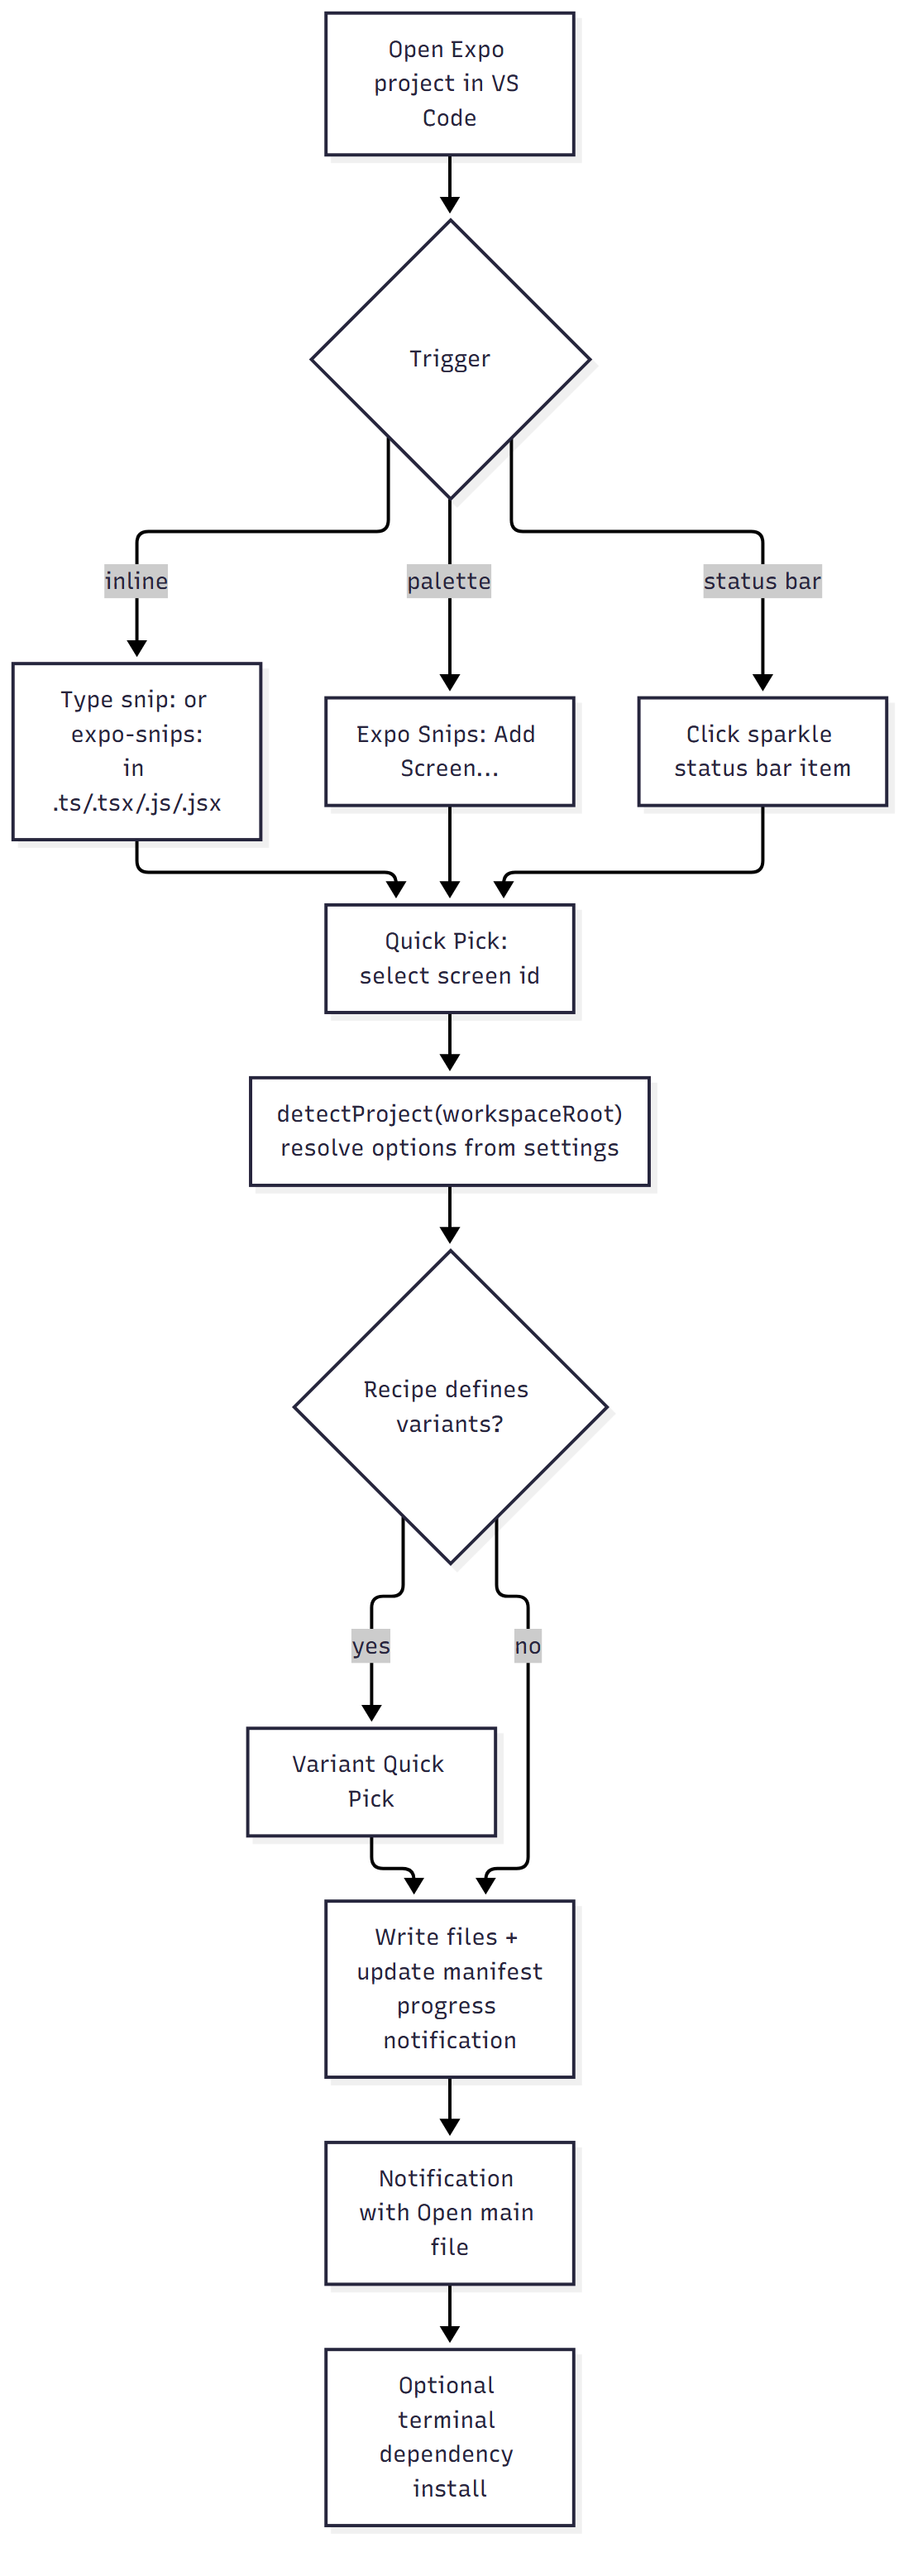
\includegraphics[width=0.95\textwidth]{diagrams/user-flow-vscode.png}
\caption{VS Code extension interaction flow}
\label{fig:user-flow-vscode}
\end{figure}

\subsection*{Activation}

The extension declares four activation events
(\texttt{packages/vscode-extension/package.json}, lines 74--80):
\texttt{onCommand:expo-snips.addScreen} and \texttt{onLanguage:} for TypeScript,
TypeScript React, JavaScript and JavaScript React. It therefore activates when a
relevant file is opened or when the command is invoked first.

\subsection*{Surfaces}

\begin{enumerate}
  \item \textbf{Inline completion.} Registered for the four language ids and
        triggered on the \texttt{:} character. The provider inspects the text before
        the cursor; on a match it produces one completion item per catalog entry,
        labelled with the recipe id and described with the recipe name,
        documentation and tags. Because \texttt{insertText} is empty and the item
        carries a command, selecting it triggers generation rather than inserting
        text.
  \item \textbf{Command palette.} \texttt{Expo Snips: Add Screen...} (declared in
        \texttt{contributes.commands}) opens a Quick Pick with matching on
        description enabled.
  \item \textbf{Status bar.} A right-aligned item at priority 100, showing the
        \texttt{sparkle} codicon and the text ``Expo Snips'', tooltip ``Add an Expo
        Snip screen'', bound to the add-screen command.
  \item \textbf{Post-generation notification.} Reports the recipe name and file
        count and offers a single action, ``Open main file'', which opens the first
        written path.
\end{enumerate}

\subsection*{Command identifiers}

\begin{table}[H]
\centering
\caption{VS Code command identifiers}
\begin{tabular}{p{6cm}p{7.6cm}}
\toprule
\textbf{Command id} & \textbf{Declared in \texttt{contributes.commands}?} \\
\midrule
\texttt{expo-snips.addScreen} & yes \\
\texttt{expo-snips.generateFromCompletion} & no --- registered at runtime only \\
\bottomrule
\end{tabular}
\end{table}

The second command is intentionally internal (it exists so completion items can
dispatch a generation). Because it is not contributed, it is invisible in the
command palette, which is the desired behaviour.

\subsection*{Progress and feedback}

Generation runs inside \texttt{vscode.window.withProgress} with a notification
location and the title ``Expo Snips: generating \{recipe name\}...'', so file writes
and primitive resolution are covered by a progress indicator.

\section{Shared client concerns}

\subsection*{Project detection}

Both clients implement the same five probes. The implementations are separate
files with near-identical bodies (\texttt{cli/src/utils/detectProject.ts} and
\texttt{vscode-extension/src/project.ts}). Only \texttt{dependencies} is inspected;
packages present solely under \texttt{devDependencies} are not detected.

\subsection*{Registry access}

Both clients:
\begin{itemize}
  \item keep an embedded catalog as the default;
  \item accept a base URL from different sources (flag/env for the CLI, a setting
        for the extension);
  \item normalise the base by trimming and stripping trailing slashes;
  \item use a 10-second abort timeout;
  \item fall back to the embedded catalog on any failure.
\end{itemize}

Differences: the extension caches and backs off; the CLI does not cache.

\subsection*{Manifest}

Both clients read and upsert \texttt{.expo-snips.json} with the same shape and the
same upsert key. The extension does not implement version bumping because it has
no update command.

\section{Presentation layer of generated screens}

Generated screens are React Native components. Their structure --- components,
styles, states and interactions --- is documented as a design system in
Chapter~\ref{ch:design-system}. The templates consistently follow a
presentational split:

\begin{itemize}
  \item a \textbf{screen} file (route-level, handles layout, safe area and
        keyboard avoidance);
  \item a \textbf{form or list item component} (encapsulates field or row
        rendering);
  \item a \textbf{hook} where async behaviour exists (for example
        \texttt{useLogin}, \texttt{useRegister});
  \item inline sample data constants (for example \texttt{stats},
        \texttt{upcoming}, product arrays) that the developer replaces.
\end{itemize}

This is IMPLEMENTED and observable across \texttt{packages/registry/templates/**}.


% ---------------------------------------------------------------------
%  Part IV: Interfaces and behaviour
% ---------------------------------------------------------------------
\chapter{CLI Reference}
\label{ch:cli-reference}

\section{Invocation}

\begin{lstlisting}[language=bash]
expo-snips <command> [options]
\end{lstlisting}

The binary is declared as \texttt{expo-snips} in
\texttt{packages/cli/package.json} (\texttt{bin}), and the program name and
description are set in \texttt{packages/cli/src/index.ts}:

\begin{lstlisting}[language=JavaScript]
program
  .name("expo-snips")
  .description("Beautiful React Native screens, one command away.")
  .version("0.1.0");
\end{lstlisting}

\textbf{Note.} The version string is hard-coded in the source rather than read from
\texttt{package.json}, so it must be kept in sync manually (see
Chapter~\ref{ch:technical-debt}).

\section{Command summary}

\begin{longtable}{p{2.1cm}p{3.1cm}p{8.6cm}}
\caption{Command summary}\\
\toprule
\textbf{Command} & \textbf{Argument} & \textbf{Purpose} \\
\midrule

\texttt{init} & none & Create a new Expo project using \texttt{create-expo-app}. \\
\texttt{list} & none & List all available screens from the resolved catalog. \\
\texttt{add} & \texttt{[screenId]} & Generate a screen into the current project. \\
\texttt{update} & \texttt{[screenId]} & Update tracked screens to the latest recipe versions. \\
\texttt{status} & none & Show screens tracked by \texttt{.expo-snips.json}. \\
\bottomrule
\end{longtable}

\section{\texttt{expo-snips init}}

\begin{lstlisting}[language=bash]
expo-snips init [--name <name>] [--template <template>]
\end{lstlisting}

\begin{longtable}{p{2.6cm}p{1.6cm}p{10.4cm}}
\caption{\texttt{init} options}\\
\toprule
\textbf{Option} & \textbf{Default} & \textbf{Behaviour} \\
\midrule

\texttt{--name <name>} & unset & Project directory name; when unset the argument
\texttt{.} is used (current directory). \\
\texttt{--template <template>} & \texttt{default} & Passed to
\texttt{create-expo-app} as \texttt{--template <template>}. \\
\bottomrule
\end{longtable}

Behaviour: if \texttt{app.json} already exists in the current working directory the
command prints ``An Expo project already exists in this directory.'' and returns
without doing anything. Otherwise it executes:

\begin{lstlisting}[language=bash]
npx create-expo-app@latest <name|.> --template <template> --yes
\end{lstlisting}

with inherited stdio, then prints next-step guidance. No exit code other than 0 is
set by this command; a failure inside \texttt{create-expo-app} propagates as a
process error from \texttt{execSync}.

\section{\texttt{expo-snips list}}

\begin{lstlisting}[language=bash]
expo-snips list [--registry <url>]
\end{lstlisting}

Resolves the catalog, reports the source (``remote''/``local''), and prints one
line per recipe: the id padded to 24 characters, the display name, and the tags in
square brackets when present.

\begin{lstlisting}[language=bash]
Available screens (24) from local registry:

  app/home                 Home Dashboard Screen [app, home, dashboard]
  auth/login               Login Screen [auth, login, form]
  ...
\end{lstlisting}

Printing an empty catalog prints ``No screens found in the registry.'' and returns
success. See Section~\ref{sec:list-empty} for the discrepancy between this
behaviour and the interactive picker's behaviour.

\section{\texttt{expo-snips add}}

\begin{lstlisting}[language=bash]
expo-snips add [screenId] [options]
\end{lstlisting}

\begin{longtable}{p{3.4cm}p{2.9cm}p{8.5cm}}
\caption{\texttt{add} options}\\
\toprule
\textbf{Option} & \textbf{Value set} & \textbf{Behaviour} \\
\midrule

\texttt{--styling <styling>} & nativewind, stylesheet, tamagui & Explicit styling; rejected when the recipe does not support it. \\
\texttt{--router <router>} & expo-router, react-navigation & Explicit router; rejected when unsupported. \\
\texttt{--ui <ui>} & native, shadcn, custom & Explicit UI primitives; rejected when unsupported. \\
\texttt{--icons <icons>} & lucide, vector-icons, none & Explicit icon library; rejected when unsupported. \\
\texttt{--variant <variant>} & recipe-defined & Screen variant id (for example \texttt{glass}). \\
\texttt{--typescript} & flag & Force TypeScript. \\
\texttt{--javascript} & flag & Force JavaScript (takes precedence over \texttt{--typescript}). \\
\texttt{--no-install} & flag & Skip dependency installation. \\
\texttt{--registry <url>} & URL & Remote registry base; defaults to \texttt{EXPO\_SNIPS\_REGISTRY}. \\
\bottomrule
\end{longtable}

\textbf{Rejected values.} A value that the recipe does not list in
\texttt{supported} aborts with a red error and exit code 1. This applies to
\texttt{--styling}, \texttt{--router}, \texttt{--ui} and \texttt{--icons}.

\textbf{Effective-value notices.} Selecting \texttt{--ui shadcn} prints a note and
overrides \texttt{styling} to \texttt{nativewind} and \texttt{icons} to
\texttt{lucide}, whether or not those were supplied explicitly. A TypeScript
recipe generated with \texttt{--javascript} prints a warning but proceeds.

\subsection*{Examples}

\begin{lstlisting}[language=bash]
# Interactive: pick a screen from a list
expo-snips add

# Named screen, defaults from project detection
expo-snips add auth/login

# Force NativeWind and no dependency installation
expo-snips add app/home --styling nativewind --no-install

# shadcn-style UI (forces nativewind + lucide; adds ui primitives)
expo-snips add auth/register --ui shadcn

# Glassmorphism variant
expo-snips add app/home --variant glass

# JavaScript output
expo-snips add auth/login --javascript

# Point at a locally served registry
expo-snips add app/home --registry http://localhost:3000
\end{lstlisting}

\textbf{Variant availability.} \texttt{--variant glass} has an effect only for
recipes that declare a \texttt{glass} variant: \texttt{app/home},
\texttt{auth/login} and \texttt{onboarding/welcome}. For any other recipe the flag
is accepted but produces default output, because the variant override map is empty.

\section{\texttt{expo-snips update}}

\begin{lstlisting}[language=bash]
expo-snips update [screenId] [--registry <url>] [--yes]
\end{lstlisting}

\begin{longtable}{p{3.4cm}p{2.9cm}p{8.5cm}}
\caption{\texttt{update} options}\\
\toprule
\textbf{Option} & \textbf{Value set} & \textbf{Behaviour} \\
\midrule

\texttt{[screenId]} & recipe id & Update only this recipe; error when no tracked
entry matches. \\
\texttt{--registry <url>} & URL & Remote registry base. \\
\texttt{--yes} & flag & Apply without the confirmation prompt. \\
\bottomrule
\end{longtable}

Behaviour:

\begin{itemize}
  \item No tracked screens: prints guidance to use \texttt{add} and returns.
  \item Nothing changed: prints ``All tracked screens are up to date.''
  \item Changes found: prints the file count, a coloured diff per changed file, then
        a confirmation prompt defaulting to \emph{no}; declining prints ``Update
        cancelled.''
  \item Applied: rewrites the files and prints the number of updated screens.
  \item A tracked recipe missing from the registry is skipped with a warning.
\end{itemize}

\begin{lstlisting}[language=bash]
expo-snips update
expo-snips update auth/login
expo-snips update --yes
\end{lstlisting}

\textbf{Important behaviour.} \texttt{update} compares the newly rendered content
with the file currently on disk. If the developer has edited a generated file, the
update will overwrite those edits once applied. The diff is the only safeguard.

\section{\texttt{expo-snips status}}

\begin{lstlisting}[language=bash]
expo-snips status
\end{lstlisting}

Reads \texttt{.expo-snips.json} from the current working directory and prints each
entry as \texttt{<recipeId padded to 24> v<recipeVersion>} with an optional
\texttt{(variant: <id>)} suffix, followed by a hint to run
\texttt{expo-snips update}.

\begin{lstlisting}[language=bash]
Tracked screens (2):

  auth/login               v0.3.0
  app/home                 v0.1.0 (variant: glass)

Run expo-snips update to update them to the latest version.
\end{lstlisting}

With no tracked screens it prints ``No screens tracked in this project yet.''

\section{Exit codes and error messages}

\begin{longtable}{p{4.4cm}p{9.6cm}}
\caption{Failure conditions and messages}\\
\toprule
\textbf{Condition} & \textbf{Message and exit code} \\
\midrule

Interactive selection cancelled & no message; exit code 1. \\
Screen id not found (\texttt{add}) & ``Screen not found: <id>'' plus a pointer to
\texttt{list}; exit code 1. \\
Option unsupported by recipe & ``Recipe "..." does not support <option> "...".''
exit code 1. \\
No files matched the options & ``No files matched the selected options. Nothing
generated.''; exit code 1. \\
No tracked entries for a given \texttt{update <id>} & ``No installed screens match
"<id>".'' plus pointer to \texttt{status}; exit code 1. \\
Empty catalog during interactive \texttt{add} & guidance to reinstall the CLI or
configure a registry; exit code 1. \\
Empty catalog during \texttt{list} & ``No screens found in the registry.''; exit code 0. \\
\bottomrule
\end{longtable}

\label{sec:list-empty}

\section{Version discrepancy note}

The CLI's \texttt{--version} output is the literal string \texttt{0.1.0} defined in
\texttt{src/index.ts}. The \texttt{package.json} also declares \texttt{0.1.0}, so
they currently agree; however, changing one without the other would silently
diverge. The VS Code extension avoids this class of problem by letting the editor
read the version from its manifest.

\chapter{Screen Registry and Recipe Model}
\label{ch:registry-and-recipes}

\section{Concept}

The registry is a catalogue of \emph{screen recipes}. A recipe is pure data: it
declares what a screen is called, which stacks it supports, which npm packages it
needs, and which files it produces. Files are produced by rendering Handlebars
templates, and a recipe may define multiple entries for the same output path, each
guarded by a \texttt{when} condition, so that one recipe yields stack-specific
output.

\section{Recipe schema}

The schema is defined in \texttt{packages/registry/schema.json} (JSON Schema
Draft-07) and mirrored by the TypeScript interface in
\texttt{packages/core/src/types.ts}.

\begin{longtable}{p{2.7cm}p{2.1cm}p{2cm}p{7.2cm}}
\caption{Recipe fields}\\
\toprule
\textbf{Field} & \textbf{Type} & \textbf{Required} & \textbf{Description} \\
\midrule

\texttt{id} & string & yes & Pattern \texttt{\^{}[a-z0-9-]+/[a-z0-9-]+\$}; must equal the
file path relative to \texttt{data/} without the extension. \\
\texttt{name} & string & yes & Human-readable name, min length 3. \\
\texttt{description} & string & yes & Short description, min length 10. \\
\texttt{version} & string & yes & Semver pattern \texttt{\^{}\textbackslash d+\textbackslash.\textbackslash d+\textbackslash.\textbackslash d+\$}. \\
\texttt{framework} & enum & yes & Only \texttt{"react-native"}. \\
\texttt{runtime} & enum & yes & Only \texttt{"expo"}. \\
\texttt{typescript} & boolean & no & Whether the recipe is authored TypeScript-first. \\
\texttt{supported} & object & yes & Four option arrays: styling, router, ui, icons. \\
\texttt{dependencies} & string[] & yes & npm packages installed with \texttt{add}. \\
\texttt{devDependencies} & string[] & no & npm packages installed with \texttt{add -D}. \\
\texttt{files} & array & yes & File entries (see below), min 1 item. \\
\texttt{variants} & array & no & Named variants, each \texttt{\{id, label, description?\}}. \\
\texttt{tags} & string[] & no & Search keywords. \\
\texttt{primitives} & string[] & no & Primitive recipe ids required when
\texttt{ui === "shadcn"}. \\
\bottomrule
\end{longtable}

\subsection*{File entry}

\begin{longtable}{p{2.7cm}p{11.1cm}}
\caption{File entry fields}\\
\toprule
\textbf{Field} & \textbf{Meaning} \\
\midrule

\texttt{path} & Output path relative to the project root. \\
\texttt{template} & Inline Handlebars template string (used at render time). \\
\texttt{templateFile} & Path to a \texttt{.hbs} file, relative to
\texttt{packages/registry/templates}; inlined into \texttt{template} at build
time and the field is deleted from the emitted recipe. \\
\texttt{perStyling} & Map from styling option to a template string or \texttt{.hbs}
path (inlined at build time). \\
\texttt{when} & Condition object with optional \texttt{styling}, \texttt{router},
\texttt{ui}, \texttt{icons} arrays and \texttt{typescript} boolean. \\
\texttt{variants} & Map from variant id to a template string or \texttt{.hbs} path
(inlined at build time). \\
\bottomrule
\end{longtable}

\subsection*{Enumerations}

\begin{table}[H]
\centering
\caption{Option enumerations (from the schema and the core types)}
\begin{tabular}{p{3cm}p{10.8cm}}
\toprule
\textbf{Option} & \textbf{Allowed values} \\
\midrule
styling & \texttt{nativewind}, \texttt{stylesheet}, \texttt{tamagui} \\
router & \texttt{expo-router}, \texttt{react-navigation} \\
ui & \texttt{native}, \texttt{shadcn}, \texttt{custom} \\
icons & \texttt{lucide}, \texttt{vector-icons}, \texttt{none} \\
\bottomrule
\end{tabular}
\end{table}

\textbf{Implementation gap.} \texttt{tamagui}, \texttt{vector-icons} and
\texttt{custom} are legal per the schema and the type unions, and are offered in VS
Code settings, but \emph{no recipe declares them}, and the CLI prompt lists only
\texttt{nativewind}/\texttt{stylesheet} and \texttt{lucide}/\texttt{none}. See
Chapter~\ref{ch:known-issues}.

\section{Catalog statistics}

\begin{table}[H]
\centering
\caption{Catalog composition (verified)}
\begin{longtable}{p{3.2cm}p{1.6cm}p{9cm}}
\toprule
\textbf{Category} & \textbf{Recipes} & \textbf{Ids} \\
\midrule
\endhead
app & 5 & \texttt{app/home}, \texttt{app/notifications}, \texttt{app/profile},
\texttt{app/search}, \texttt{app/settings} \\
auth & 4 & \texttt{auth/login}, \texttt{auth/register},
\texttt{auth/forgot-password}, \texttt{auth/otp-verification} \\
calendar & 1 & \texttt{calendar/schedule} \\
chat & 1 & \texttt{chat/conversations} \\
content & 1 & \texttt{content/article-reader} \\
dashboard & 1 & \texttt{dashboard/analytics} \\
ecommerce & 2 & \texttt{ecommerce/products}, \texttt{ecommerce/product-details} \\
map & 1 & \texttt{map/location} \\
onboarding & 3 & \texttt{onboarding/welcome}, \texttt{onboarding/features},
\texttt{onboarding/permissions} \\
ui & 3 & \texttt{ui/button}, \texttt{ui/input}, \texttt{ui/utils} \\
utility & 2 & \texttt{utility/empty}, \texttt{utility/error} \\
\midrule
\textbf{Total} & \textbf{24} & --- \\
\bottomrule
\end{longtable}
\end{table}

Templates: \textbf{48} \texttt{.hbs} files under
\texttt{packages/registry/templates}, organised by the same category structure.

\section{Variants}

Only three recipes declare a variant, all with the id \texttt{glass} and label
``Glassmorphism'':
\texttt{app/home} (\texttt{app.home.index.glass.hbs}),
\texttt{auth/login} (\texttt{app.login.index.glass.hbs}) and
\texttt{onboarding/welcome} (\texttt{app.welcome.index.glass.hbs}).

The remaining twenty-one recipes declare \texttt{"variants": []}.

The glass templates render a dark surface (\texttt{\#0F172A}) with translucent
overlays (\texttt{rgba(255,255,255,0.08)}) and, for \texttt{auth/login}, import
\texttt{BlurView} from \texttt{expo-blur}; note that \texttt{expo-blur} is not
declared in that recipe's \texttt{dependencies} array (see
Chapter~\ref{ch:known-issues}).

\section{Template organisation}

\begin{lstlisting}[language=bash]
packages/registry/templates/
  app/home/app.home.index.hbs
  app/home/app.home.index.glass.hbs
  auth/login/app.login.index.hbs
  auth/login/app.login.index.shadcn.hbs
  auth/login/app.login.index.glass.hbs
  auth/login/components.login-form.hbs
  auth/login/components.login-form.shadcn.hbs
  auth/login/screens.loginscreen.react-navigation.hbs
  auth/login/hooks.use-login.hbs
  ui/button.hbs
  ui/input.hbs
  ui/lib.utils.hbs
  ...
\end{lstlisting}

The naming convention is \texttt{<path-with-dots>.<variant-suffix>.hbs}, for
example \texttt{components.login-form.shadcn.hbs} for the shadcn variant of
\texttt{components/LoginForm.tsx}.

\section{Build and distribution}

\begin{figure}[H]
\centering
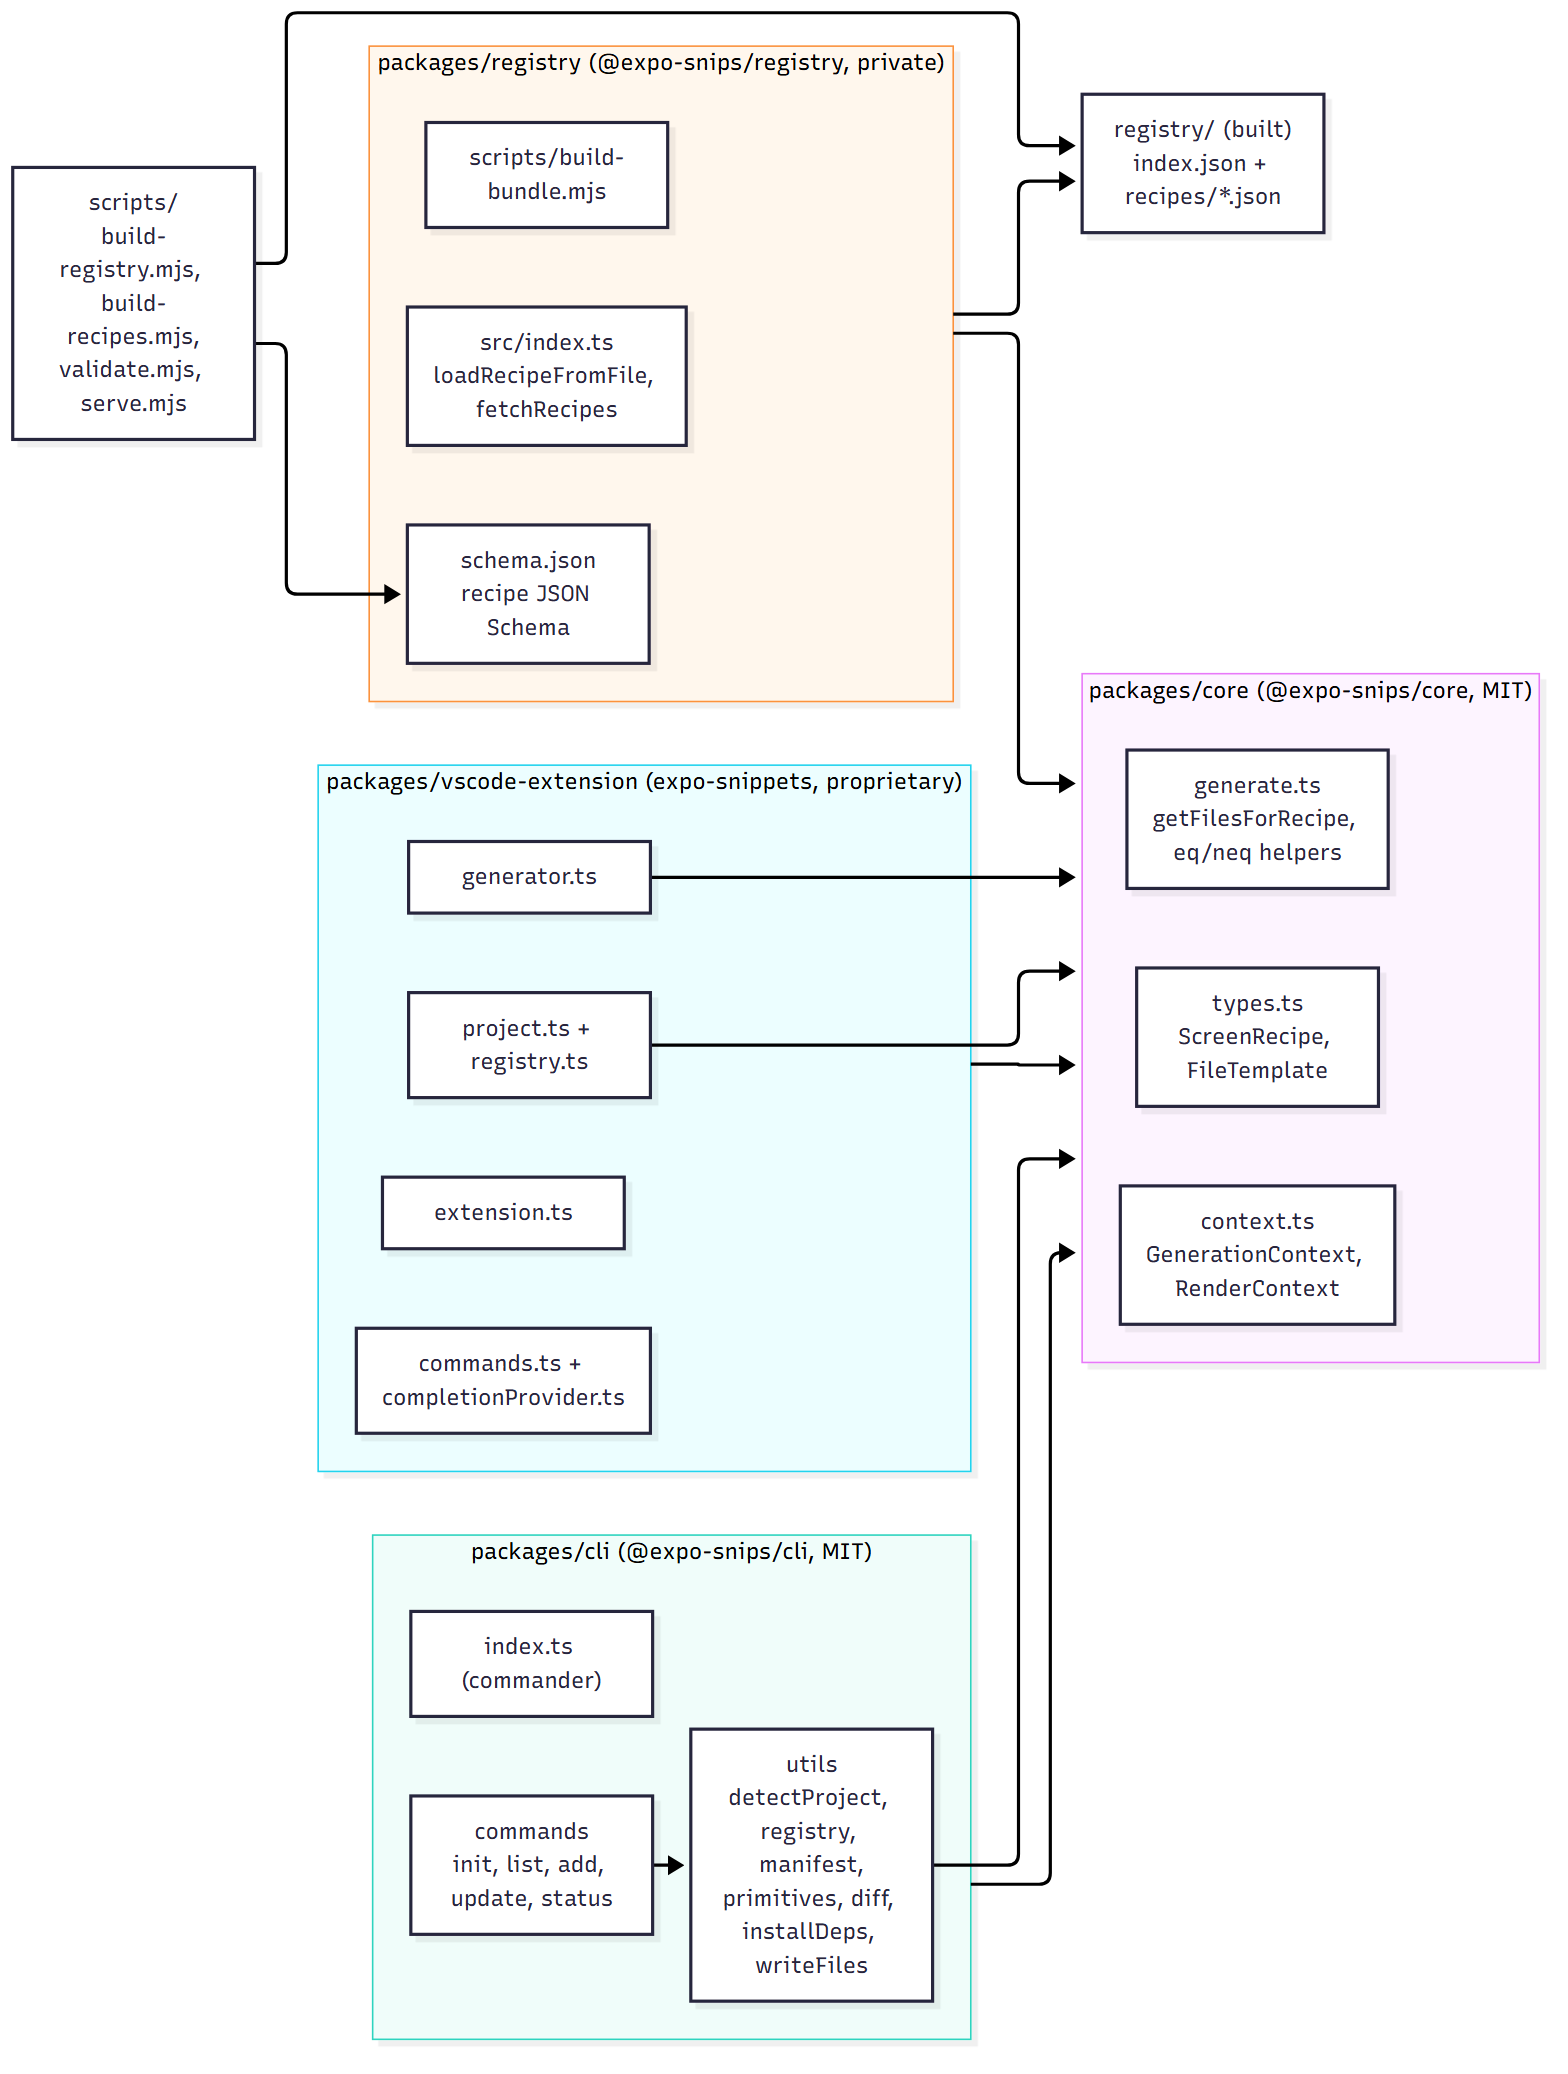
\includegraphics[width=0.98\textwidth]{diagrams/component-architecture.png}
\caption{Recipe data flows into the built registry and into the embedded client bundles}
\label{fig:registry-build}
\end{figure}

\begin{longtable}{p{4.6cm}p{9.4cm}}
\caption{Build outputs derived from the recipe sources}\\
\toprule
\textbf{Output} & \textbf{Producer and purpose} \\
\midrule

\texttt{registry/index.json} & \texttt{scripts/build-registry.mjs}. Index entries for
all 24 recipes; served at \texttt{\{base\}/index.json}. \\
\texttt{registry/recipes/<id>.json} & \texttt{scripts/build-registry.mjs}. Full
recipes with inlined templates; served at \texttt{\{base\}/recipes/<id>.json}. \\
\texttt{packages/registry/bundle.json} & \texttt{scripts/build-bundle.mjs}. A
\texttt{\{version:1, name, recipes\}} bundle for offline consumption. \\
\texttt{packages/cli/src/generated/registry-data.ts} & \texttt{scripts/prepare-registry.mjs}.
Embedded catalog for the CLI. \\
\texttt{packages/vscode-extension/src/generated/registry-data.ts} & Same script;
embedded catalog for the extension. \\
\bottomrule
\end{longtable}

All four derived outputs are produced from the single source of truth in
\texttt{packages/registry/data} and \texttt{packages/registry/templates}. The
generated per-client modules are git-ignored
(\texttt{.gitignore}, lines 7--8). The built \texttt{registry/} folder is committed
and is rebuilt (deleted first) by the build script.

\section{Validation}

\texttt{scripts/validate.mjs} (run with \texttt{pnpm validate}) implements a
hand-written subset of JSON Schema Draft-07 validation. For each file under
\texttt{data/} it checks:

\begin{itemize}
  \item all required fields are present;
  \item \texttt{id} matches \texttt{\^{}[a-z0-9-]+/[a-z0-9-]+\$};
  \item \texttt{version} matches the three-part semver pattern;
  \item \texttt{framework} is \texttt{react-native} and \texttt{runtime} is
        \texttt{expo};
  \item every \texttt{supported.*} value is a legal enum member;
  \item \texttt{files} is a non-empty array and every entry has both \texttt{path}
        and \texttt{templateFile};
  \item \texttt{id} equals the file's path relative to \texttt{data/};
  \item every referenced template file exists on disk.
\end{itemize}

It prints a per-recipe pass/fail line and exits non-zero when any error is found.
It is the only automated verification in the repository.

\textbf{Note.} Because the emitted recipes replace \texttt{templateFile} with
\texttt{template}, validation must run against the \emph{source} data directory;
the validator is invoked by \texttt{pnpm validate} precisely for that reason.

\chapter{API Documentation}
\label{ch:api-documentation}

The system exposes three classes of interface:

\begin{enumerate}
  \item the \textbf{registry HTTP interface} (read-only static JSON);
  \item the \textbf{programmatic interfaces} of the published packages;
  \item the \textbf{CLI interface}, documented in Chapter~\ref{ch:cli-reference}.
\end{enumerate}

There is no authenticated API, no write API and no server-side application.

\section{Registry HTTP interface}

\subsection*{Base URL resolution}

\begin{longtable}{p{4.2cm}p{10cm}}
\caption{Registry base URL resolution}\\
\toprule
\textbf{Consumer} & \textbf{Resolution chain} \\
\midrule

CLI & \texttt{--registry <url>} flag $\rightarrow$ \texttt{EXPO\_SNIPS\_REGISTRY}
environment variable $\rightarrow$ empty (embedded catalog). \\
Extension & \texttt{expo-snips.registryUrl} setting $\rightarrow$ empty (embedded
catalog). \\
Declared default constant & \texttt{https://registry.expo-snips.dev}
(\texttt{DEFAULT\_REGISTRY} in both clients) --- exported but not used as an
implicit default; an empty base selects the embedded catalog. \\
Dev server & \texttt{pnpm serve} $\rightarrow$ \texttt{http://localhost:3000}. \\
\bottomrule
\end{longtable}

The base is normalised by trimming whitespace and removing trailing slashes.

\subsection*{\texttt{GET /index.json}}

\begin{longtable}{p{3.4cm}p{10.8cm}}
\toprule
\textbf{Aspect} & \textbf{Detail} \\
\midrule
\textbf{Purpose} & Return the catalog index used for browsing and selection. \\
\textbf{Method} & GET \\
\textbf{Authentication} & None. \\
\textbf{Authorization} & None (public read). \\
\textbf{Headers} & None required. \\
\textbf{Parameters} & None. \\
\textbf{Request body} & None. \\
\textbf{Response} & JSON array of index entries. \\
\textbf{Timeout} & Client-side abort after 10\,000\,ms. \\
\textbf{Status codes} & Any non-2xx is treated as failure by the client
(\texttt{response.ok} check); the client then falls back to the embedded catalog. \\
\textbf{Validation} & The client accepts the payload only when it is an array with
at least one element. \\
\textbf{Source} & Produced by \texttt{scripts/build-registry.mjs} via
\texttt{toIndexEntry}. \\
\bottomrule
\end{longtable}

Index entry shape:

\begin{lstlisting}[language=JavaScript]
interface RecipeIndexEntry {
  id: string;          // e.g. "auth/login"
  name: string;        // e.g. "Login Screen"
  description: string;
  version: string;     // semver, e.g. "0.3.0"
  typescript: boolean;
  tags: string[];
  supported: {
    styling: string[];
    router: string[];
    ui: string[];
    icons: string[];
  };
}
\end{lstlisting}

Example response fragment (from \texttt{registry/index.json}):

\begin{lstlisting}[language=JavaScript]
[
  {
    "id": "app/home",
    "name": "Home Dashboard Screen",
    "description": "Home screen with greeting, stats cards and upcoming tasks list.",
    "version": "0.1.0",
    "typescript": true,
    "tags": ["app", "home", "dashboard"],
    "supported": {
      "styling": ["nativewind", "stylesheet"],
      "router": ["expo-router"],
      "ui": ["native"],
      "icons": ["lucide", "none"]
    }
  }
]
\end{lstlisting}

\textbf{Note.} The index omits \texttt{variants}, so clients browsing only the
index cannot tell whether a recipe offers variants. Only the full recipe document
carries them.

\subsection*{\texttt{GET /recipes/\{id\}.json}}

\begin{longtable}{p{3.4cm}p{10.8cm}}
\toprule
\textbf{Aspect} & \textbf{Detail} \\
\midrule
\textbf{Purpose} & Return one complete recipe with templates inlined. \\
\textbf{Method} & GET \\
\textbf{Path parameter} & Recipe id, URL-encoded by the client
(\texttt{encodeURIComponent}); note that the on-disk path uses a slash
(\texttt{recipes/auth/login.json}) while the client encodes the slash as
\texttt{\%2F}. \\
\textbf{Authentication} & None. \\
\textbf{Response} & A \texttt{ScreenRecipe} object with \texttt{files[].template}
strings. \\
\textbf{Client acceptance} & Accepted only when the payload is an object with a
truthy \texttt{id}. \\
\textbf{Fallback} & Embedded catalog lookup by id. \\
\textbf{Source} & Written by \texttt{scripts/build-registry.mjs} to
\texttt{registry/recipes/<id>.json}. \\
\bottomrule
\end{longtable}

Example (abridged) response:

\begin{lstlisting}[language=JavaScript]
{
  "id": "auth/login",
  "name": "Login Screen",
  "version": "0.3.0",
  "framework": "react-native",
  "runtime": "expo",
  "typescript": true,
  "supported": {
    "styling": ["nativewind", "stylesheet"],
    "router": ["expo-router", "react-navigation"],
    "ui": ["native", "shadcn"],
    "icons": ["lucide", "none"]
  },
  "dependencies": ["react-hook-form", "zod", "@hookform/resolvers", "lucide-react-native"],
  "files": [
    {
      "path": "app/login/index.tsx",
      "when": { "router": ["expo-router"], "ui": ["native"] },
      "variants": { "glass": "import { ... } from 'react-native'; ..." },
      "template": "import { View, Text, ... } from 'react-native'; ..."
    }
  ],
  "variants": [{ "id": "glass", "label": "Glassmorphism", "description": "..." }],
  "tags": ["auth", "login", "form"],
  "primitives": ["ui/utils", "ui/button", "ui/input"]
}
\end{lstlisting}

\subsection*{Local development server}

\texttt{scripts/serve.mjs} starts a Node \texttt{http} server that serves the built
\texttt{registry/} folder as static files (default port 3000, overridable with the
\texttt{PORT} environment variable). It:

\begin{itemize}
  \item answers \texttt{OPTIONS} with \texttt{204} and permissive CORS headers
        (\texttt{Access-Control-Allow-Origin: *}, methods \texttt{GET, OPTIONS});
  \item resolves the URL path against the registry root and rejects any path that
        escapes it, preventing traversal;
  \item maps directories and trailing slashes to \texttt{index.json};
  \item returns \texttt{404} with \texttt{\{"error":"Not found"\}} for unknown paths;
  \item sets a content type from a small extension map (JSON, HBS, PNG, JPG, GIF,
        SVG) and otherwise \texttt{application/octet-stream}.
\end{itemize}

It refuses to start when \texttt{registry/index.json} is missing and instructs the
operator to run \texttt{pnpm build:registry} first.

\section{Programmatic interfaces}

\subsection*{\texttt{@expo-snips/core} (MIT, published)}

\begin{longtable}{p{6.4cm}p{7.8cm}}
\caption{Public exports of the core package}\\
\toprule
\textbf{Export} & \textbf{Purpose} \\
\midrule

\texttt{renderTemplate(templateStr, context)} & Render one template to a string. \\
\texttt{getFilesForRecipe(recipe, context, resolveFile?)} & Render a recipe into
\texttt{\{path, content\}[]}. \\
\texttt{GenerationContext}, \texttt{GenerationOptions}, \texttt{RenderContext} & Input
types for rendering. \\
\texttt{ScreenRecipe}, \texttt{FileTemplate}, \texttt{ScreenVariant},
\texttt{Conditions} & Data model types. \\
\texttt{StylingOption}, \texttt{RouterOption}, \texttt{UIOption}, \texttt{IconOption} &
Option unions. \\
\bottomrule
\end{longtable}

Usage example:

\begin{lstlisting}[language=JavaScript]
import { getFilesForRecipe, GenerationContext, ScreenRecipe } from "@expo-snips/core";

const context: GenerationContext = {
  projectRoot: process.cwd(),
  options: { styling: "nativewind", router: "expo-router", ui: "native", icons: "lucide", typescript: true },
};

const files = getFilesForRecipe(recipe as ScreenRecipe, context);
// => [{ path: "app/login/index.tsx", content: "..." }, ...]
\end{lstlisting}

\subsection*{\texttt{@expo-snips/cli} (MIT, published)}

The CLI package exposes no documented programmatic API. Its
\texttt{main} points to \texttt{dist/index.js}, which executes the commander
program as a side effect when imported, so it is intended for use as a binary
rather than as a library.

\subsection*{\texttt{@expo-snips/registry} (private)}

\begin{longtable}{p{6.4cm}p{7.8cm}}
\caption{Exports of the registry package}\\
\toprule
\textbf{Export} & \textbf{Purpose} \\
\midrule

\texttt{loadRecipeFromFile(filePath)} & Parse a recipe and inline \texttt{templateFile},
variant and per-styling references. \\
\texttt{getAllRecipes()} & Recursively load and inline every recipe under
\texttt{data/}. \\
\texttt{getRecipeById(id)} & Load and match a single recipe. \\
\texttt{searchRecipes(query)} & Case-insensitive match on id, name or tags. \\
\texttt{fetchRecipes(url)} & Fetch a remote registry document; accepts a bare array,
a \texttt{\{recipes\}} bundle, or a single recipe object; throws on a non-OK
response or an unrecognised body. \\
\bottomrule
\end{longtable}

Its filesystem functions resolve paths relative to the package directory using
\texttt{\_\_dirname}, so they are only meaningful inside the repository or a
distribution that includes \texttt{data/} and \texttt{templates/}.

\subsection*{\texttt{expo-snippets} (VS Code extension, proprietary)}

Contributes one command and registers a second at runtime.

\begin{longtable}{p{5.6cm}p{8.6cm}}
\caption{Extension commands and settings contributions}\\
\toprule
\textbf{Interface} & \textbf{Definition} \\
\midrule

Command & \texttt{expo-snips.addScreen} --- title ``Expo Snips: Add Screen...''. \\
Command (runtime) & \texttt{expo-snips.generateFromCompletion(recipeId?)}. \\
Setting & \texttt{expo-snips.registryUrl} (string, default empty). \\
Setting & \texttt{expo-snips.defaultStyling} (enum, default \texttt{nativewind}). \\
Setting & \texttt{expo-snips.defaultRouter} (enum, default \texttt{expo-router}). \\
Setting & \texttt{expo-snips.defaultUi} (enum, default \texttt{native}). \\
Setting & \texttt{expo-snips.defaultIcons} (enum, default \texttt{lucide}). \\
Setting & \texttt{expo-snips.installDependencies} (boolean, default \texttt{true}). \\
Activation & \texttt{onCommand:expo-snips.addScreen} and
\texttt{onLanguage:\{typescript,\allowbreak typescriptreact,\allowbreak javascript,\allowbreak javascriptreact\}}. \\
\bottomrule
\end{longtable}

\section{Failure and error semantics summary}

\begin{longtable}{p{4.4cm}p{3.4cm}p{6.4cm}}
\caption{Error semantics across interfaces}\\
\toprule
\textbf{Failure} & \textbf{Signal} & \textbf{Client behaviour} \\
\midrule

Registry unreachable & Fetch rejects or aborts & Fall back to the embedded catalog;
CLI prints a warning when a base was configured. \\
Registry returns non-OK & \texttt{response.ok} false & Same fallback. \\
Registry returns empty array & Array length 0 & Same fallback. \\
Recipe missing & \texttt{getRecipeById} returns null & CLI: error and exit 1.
Extension: error message. \\
Manifest unreadable & JSON parse throws & Treated as empty manifest. \\
Unknown primitive id & Recipe lookup returns null & Warning; primitive skipped. \\
Install failure & Child process error & CLI aborts with the process error; files
are already written. \\
\bottomrule
\end{longtable}

\chapter{Authentication}
\label{ch:authentication}

\section{Product authentication}

\textbf{Status:} NOT APPLICABLE.

Expo Snips has no users, accounts, sessions or credentials of its own. It is a
local developer tool. A repository-wide inspection found no authentication code,
no token handling, no session storage, no OAuth client, no password logic and no
identity provider configuration in the product itself.

Consequences that follow directly from this:

\begin{itemize}
  \item The CLI requires no login and stores no credentials.
  \item The VS Code extension requires no login and stores no credentials.
  \item The registry is unauthenticated static hosting.
  \item \texttt{.expo-snips.json} contains no personal data.
  \item There is no MFA, no token lifecycle, no refresh flow and no session store
        to document. All of these are \textbf{NOT APPLICABLE}.
\end{itemize}

\section{Authentication templates generated for user applications}

The catalogue \emph{does} contain authentication \emph{screens}, which are
generated into the developer's own application. Those screens are not
authentication for Expo Snips; they are scaffolding for the developer's app.

The four auth recipes are:

\begin{longtable}{p{3.6cm}p{1.5cm}p{1.9cm}p{7.4cm}}
\caption{Authentication recipes}\\
\toprule
\textbf{Recipe} & \textbf{Version} & \textbf{UI} & \textbf{Generated files} \\
\midrule

\texttt{auth/login} & 0.3.0 & native, shadcn & \texttt{app/login/index.tsx} (or
\texttt{screens/LoginScreen.tsx} for react-navigation),
\texttt{components/LoginForm.tsx}, \texttt{hooks/useLogin.ts|.js}; optional
\texttt{glass} variant. \\
\texttt{auth/register} & 0.2.0 & native, shadcn & \texttt{app/register/index.tsx} (or
\texttt{screens/RegisterScreen.tsx}), \texttt{components/RegisterForm.tsx},
\texttt{hooks/useRegister.ts|.js}. \\
\texttt{auth/forgot-password} & 0.2.0 & native, shadcn &
\texttt{app/forgot-password/index.tsx},
\texttt{components/ForgotPasswordForm.tsx}. \\
\texttt{auth/otp-verification} & 0.2.0 & native, shadcn &
\texttt{app/otp-verification/index.tsx}, \texttt{components/OtpInput.tsx}. \\
\bottomrule
\end{longtable}

\section{Validation model in generated screens}

All form-based auth recipes use the same pattern, implemented in the templates:

\begin{itemize}
  \item \texttt{react-hook-form} with the \texttt{Controller} component for
        controlled inputs;
  \item a \texttt{zod} schema and \texttt{zodResolver} for validation;
  \item a typed form data type derived with \texttt{z.infer<typeof schema>} in the
        TypeScript path, and an untyped equivalent in the JavaScript path;
  \item per-field error text rendered from \texttt{formState.errors}.
\end{itemize}

Example schema, reproduced from
\texttt{packages/registry/templates/auth/login/components.login-form.hbs}:

\begin{lstlisting}[language=JavaScript]
const schema = z.object({
  email: z.string().email('Invalid email address'),
  password: z.string().min(6, 'Password must be at least 6 characters'),
});

type FormData = z.infer<typeof schema>;
\end{lstlisting}

The shadcn variant uses slightly different messages
(\texttt{"Email is required"}, \texttt{"Enter a valid email"},
\texttt{"Password must be at least 6 characters"}).

\section{Authentication state and flow}

\begin{figure}[H]
\centering
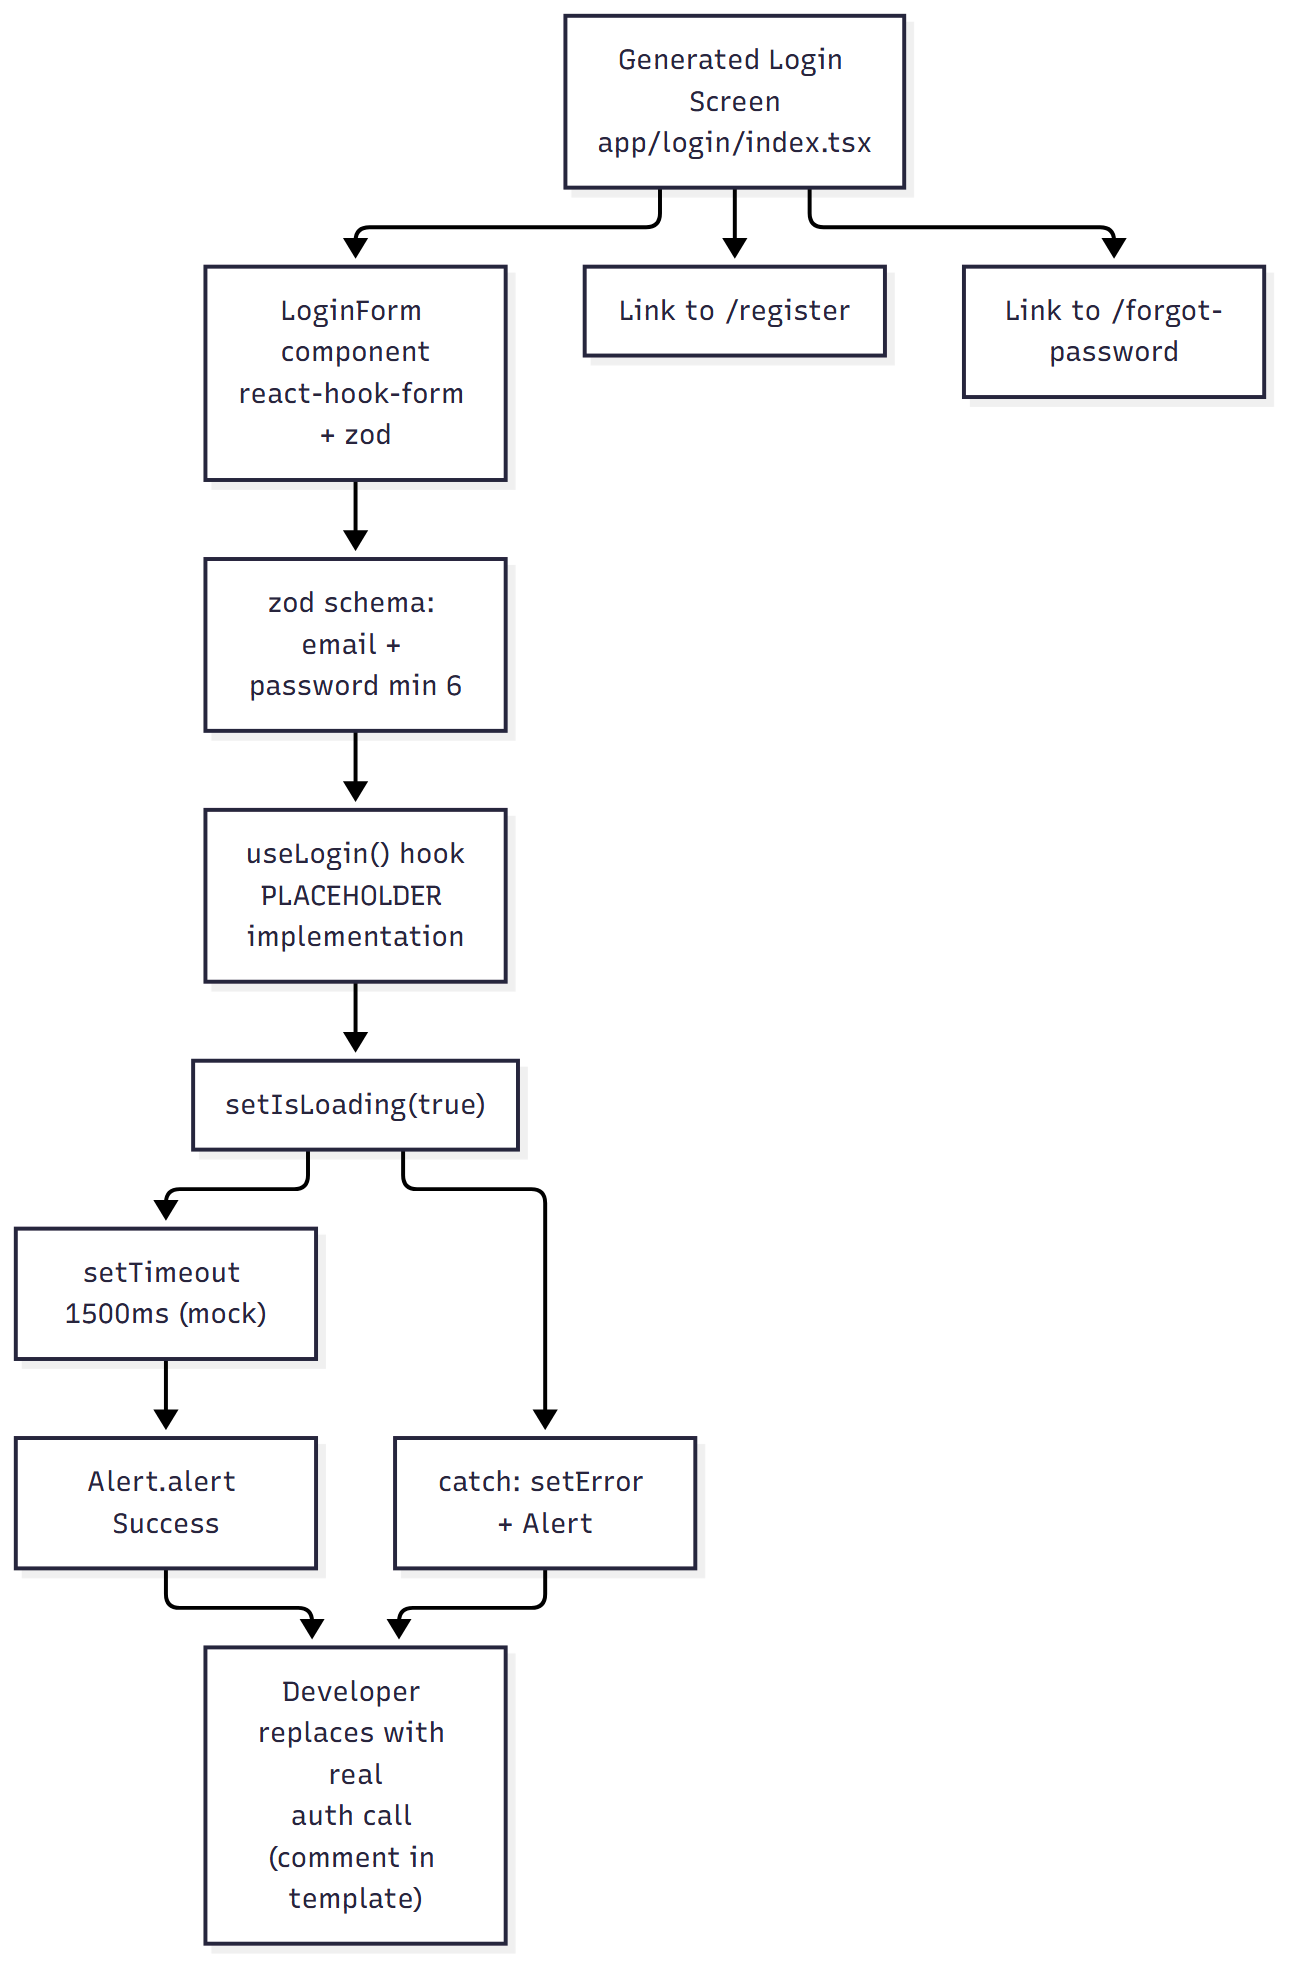
\includegraphics[width=0.78\textwidth]{diagrams/authentication-flow.png}
\caption{Authentication flow encoded in the generated templates (placeholder backend)}
\label{fig:authentication-flow}
\end{figure}

\textbf{Critical characteristic: the authentication backend is a placeholder.}
\texttt{hooks/use-login.hbs} and \texttt{hooks/use-register.hbs} implement:

\begin{itemize}
  \item \texttt{isLoading} and \texttt{error} state;
  \item a \texttt{console.log} of the submitted credentials;
  \item a mocked 1{,}500\,ms delay (\texttt{new Promise((resolve) =>
        setTimeout(resolve, 1500))});
  \item an \texttt{Alert.alert('Success', 'Logged in successfully')} on completion;
  \item a \texttt{catch} that stores the error message and shows an alert.
\end{itemize}

The template carries an explicit instruction to the developer:

\begin{lstlisting}[language=JavaScript]
// Replace with your actual authentication logic
// Example: await supabase.auth.signInWithPassword({ email, password });
\end{lstlisting}

\textbf{The shadcn variants differ materially.} The shadcn login form's
\texttt{onSubmit} simply runs \texttt{console.log(data)} --- it does not call the
\texttt{useLogin} hook at all
(\texttt{templates/auth/login/components.login-form.shadcn.hbs}). A developer
choosing \texttt{--ui shadcn} therefore receives a form with validation but no
loading or error handling from the hook. This inconsistency is recorded in
Chapter~\ref{ch:known-issues}.

\section{Password handling}

\begin{itemize}
  \item The native login form implements a secure-entry toggle: a
        \texttt{showPassword} state selects between \texttt{secureTextEntry} and an
        obscured/plain rendering, with \texttt{Eye}/\texttt{EyeOff} icons from
        \texttt{lucide-react-native}.
  \item The register recipe validates a password and a confirmation password with a
        \texttt{min(6)} rule.
  \item No password is ever persisted, hashed or transmitted by the product.
  \item The mocked hook logs the credentials to the console for demonstration; a
        developer should remove that \texttt{console.log} before shipping (see
        Chapter~\ref{ch:security}).
\end{itemize}

\textbf{Status:} IMPLEMENTED (templates) / RECOMMENDED (removing the console log).

\section{Session, token and MFA handling}

\textbf{Status:} NOT APPLICABLE.

No session storage, token issuance, refresh logic, secure storage, biometric flow,
or multi-factor authentication is present in the product, and none is generated by
default. The OTP recipe provides a one-time-code \emph{input experience}
(\texttt{components/OtpInput.tsx} with auto-advance behaviour) but contains no code
verification backend; the developer must supply that. The
\texttt{auth/otp-verification} recipe depends only on
\texttt{lucide-react-native}.

\section{Recommendations for users of the generated auth screens}

\begin{itemize}
  \item Replace the mock \texttt{useLogin}/\texttt{useRegister} bodies with a real
        authentication call (the templates suggest Supabase as an example only).
  \item Remove the credential \texttt{console.log}.
  \item Add secure storage (for example \texttt{expo-secure-store}) for any
        session token --- the templates do not include one.
  \item Wire navigation to the real post-login route; templates link to
        \texttt{/register} and \texttt{/forgot-password} by convention and do not
        perform authentication redirects.
\end{itemize}

\textbf{Status:} RECOMMENDED.

\chapter{Authorization}
\label{ch:authorization}

\section{Product authorization}

\textbf{Status:} NOT APPLICABLE.

Expo Snips implements no authorization model. There are no roles, permissions,
policies, access-control lists, middleware guards or protected resources in the
product. Relevant evidence:

\begin{itemize}
  \item The CLI has no notion of a user or a role; all subcommands are available to
        anyone who can execute the binary.
  \item The extension has no \texttt{when} activation clauses beyond command and
        language activation, and no user-dependent behaviour.
  \item The registry is public, read-only static hosting; every recipe and every
        template is readable by anyone who can reach the host.
  \item There is no role/permission data model, no RLS (the product has no
        database) and no policy engine. All \textbf{NOT APPLICABLE}.
\end{itemize}

\section{Effective privilege boundaries}

Although there is no authorization \emph{model}, the system does have privilege
boundaries that matter operationally:

\begin{longtable}{p{4.4cm}p{5.4cm}p{4.6cm}}
\caption{Effective privilege boundaries}\\
\toprule
\textbf{Boundary} & \textbf{What is possible} & \textbf{What is not} \\
\midrule

Local file writes & Generate files at any path declared by a recipe, relative to the
project root. & Read arbitrary files (the tool only reads \texttt{package.json},
\texttt{tsconfig.json}, the manifest and files it is about to overwrite). \\
Child process execution & Run the detected package manager; run \texttt{npx
create-expo-app} during \texttt{init}. & Run arbitrary commands from recipe data ---
recipe \texttt{dependencies} strings are inserted into the install command line. \\
Network access & Fetch JSON from the configured registry base. & Upload data;
transmit credentials; authenticate. \\
Registry content & Any published recipe is trusted and rendered verbatim. & Verify
provenance or signature. \\
\bottomrule
\end{longtable}

\section{A UI access consideration worth recording}

The catalog contains three recipes that are \emph{not} end-user screens but shared
UI primitives (\texttt{ui/button}, \texttt{ui/input}, \texttt{ui/utils}). They are
listed by \texttt{expo-snips list} and are selectable from the CLI picker and the
VS Code Quick Pick exactly like application screens. Nothing in the CLI prevents a
user from running:

\begin{lstlisting}[language=bash]
expo-snips add ui/button
\end{lstlisting}

which writes \texttt{components/ui/button.tsx} (and, because \texttt{ui/button}
declares \texttt{primitives: ["ui/utils"]}, also \texttt{lib/utils.ts}) directly
into the project, with \texttt{styling} forced to \texttt{nativewind} and
\texttt{ui} forced to \texttt{shadcn} by the primitive-resolution logic.

\textbf{Assessment (INFERRED).} This is not a security problem, but it is a
usability and presentation concern: internal primitives are indistinguishable from
application screens in every discovery surface. A future revision could filter
\texttt{ui/*} ids from the user-facing pickers or mark them as internal.

\section{Recommendation}

If a hosted, curated registry is ever offered, authorization will become relevant
in at least two places:

\begin{enumerate}
  \item \textbf{Write access} to publish recipes --- currently anyone with write
        access to the repository (and therefore the CI token) can publish, and
        there is no review gate beyond pull-request review.
  \item \textbf{Read access} to private/company catalogs --- the configurable
        registry has no support for authentication headers or tokens, so a private
        registry must currently be reachable without credentials (for example, on a
        trusted network or behind a proxy).
\end{enumerate}

\textbf{Status:} RECOMMENDED. Neither behaviour exists today.

\chapter{User Flows}
\label{ch:user-flows}

\section{CLI journey}

\begin{figure}[H]
\centering
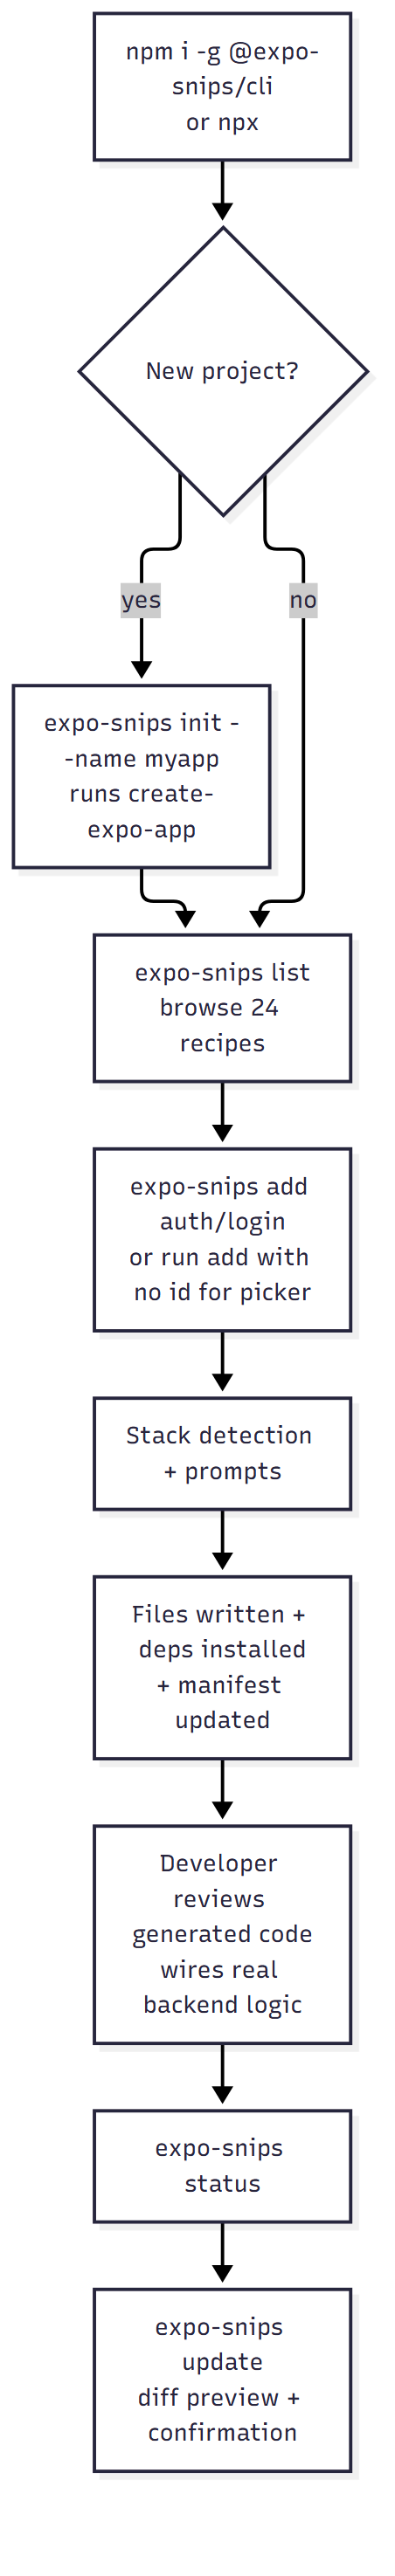
\includegraphics[width=0.92\textwidth]{diagrams/user-flow-cli.png}
\caption{CLI journey from installation to keeping screens up to date}
\label{fig:user-flow-cli}
\end{figure}

\begin{longtable}{p{1cm}p{4.2cm}p{9.2cm}}
\caption{CLI journey steps}\\
\toprule
\textbf{\#} & \textbf{Step} & \textbf{Detail} \\
\midrule

1 & Install & \texttt{npm i -g @expo-snips/cli}, or invoke through \texttt{npx}. \\
2 & (Optional) bootstrap & \texttt{expo-snips init --name myapp} runs
\texttt{create-expo-app}. \\
3 & Browse & \texttt{expo-snips list} prints 24 recipes with tags. \\
4 & Generate & \texttt{expo-snips add auth/login} (or bare \texttt{add} for a picker). \\
5 & Detect and prompt & The CLI reports detected values and prompts only for
unresolved options. \\
6 & Write and install & Files are created; recipe dependencies are installed. \\
7 & Record & \texttt{.expo-snips.json} is updated. \\
8 & Review & The developer edits the generated code and wires real logic. \\
9 & Maintain & \texttt{status} to inspect, \texttt{update} to pull catalog
improvements with a diff preview. \\
\bottomrule
\end{longtable}

\section{VS Code journey}

\begin{figure}[H]
\centering
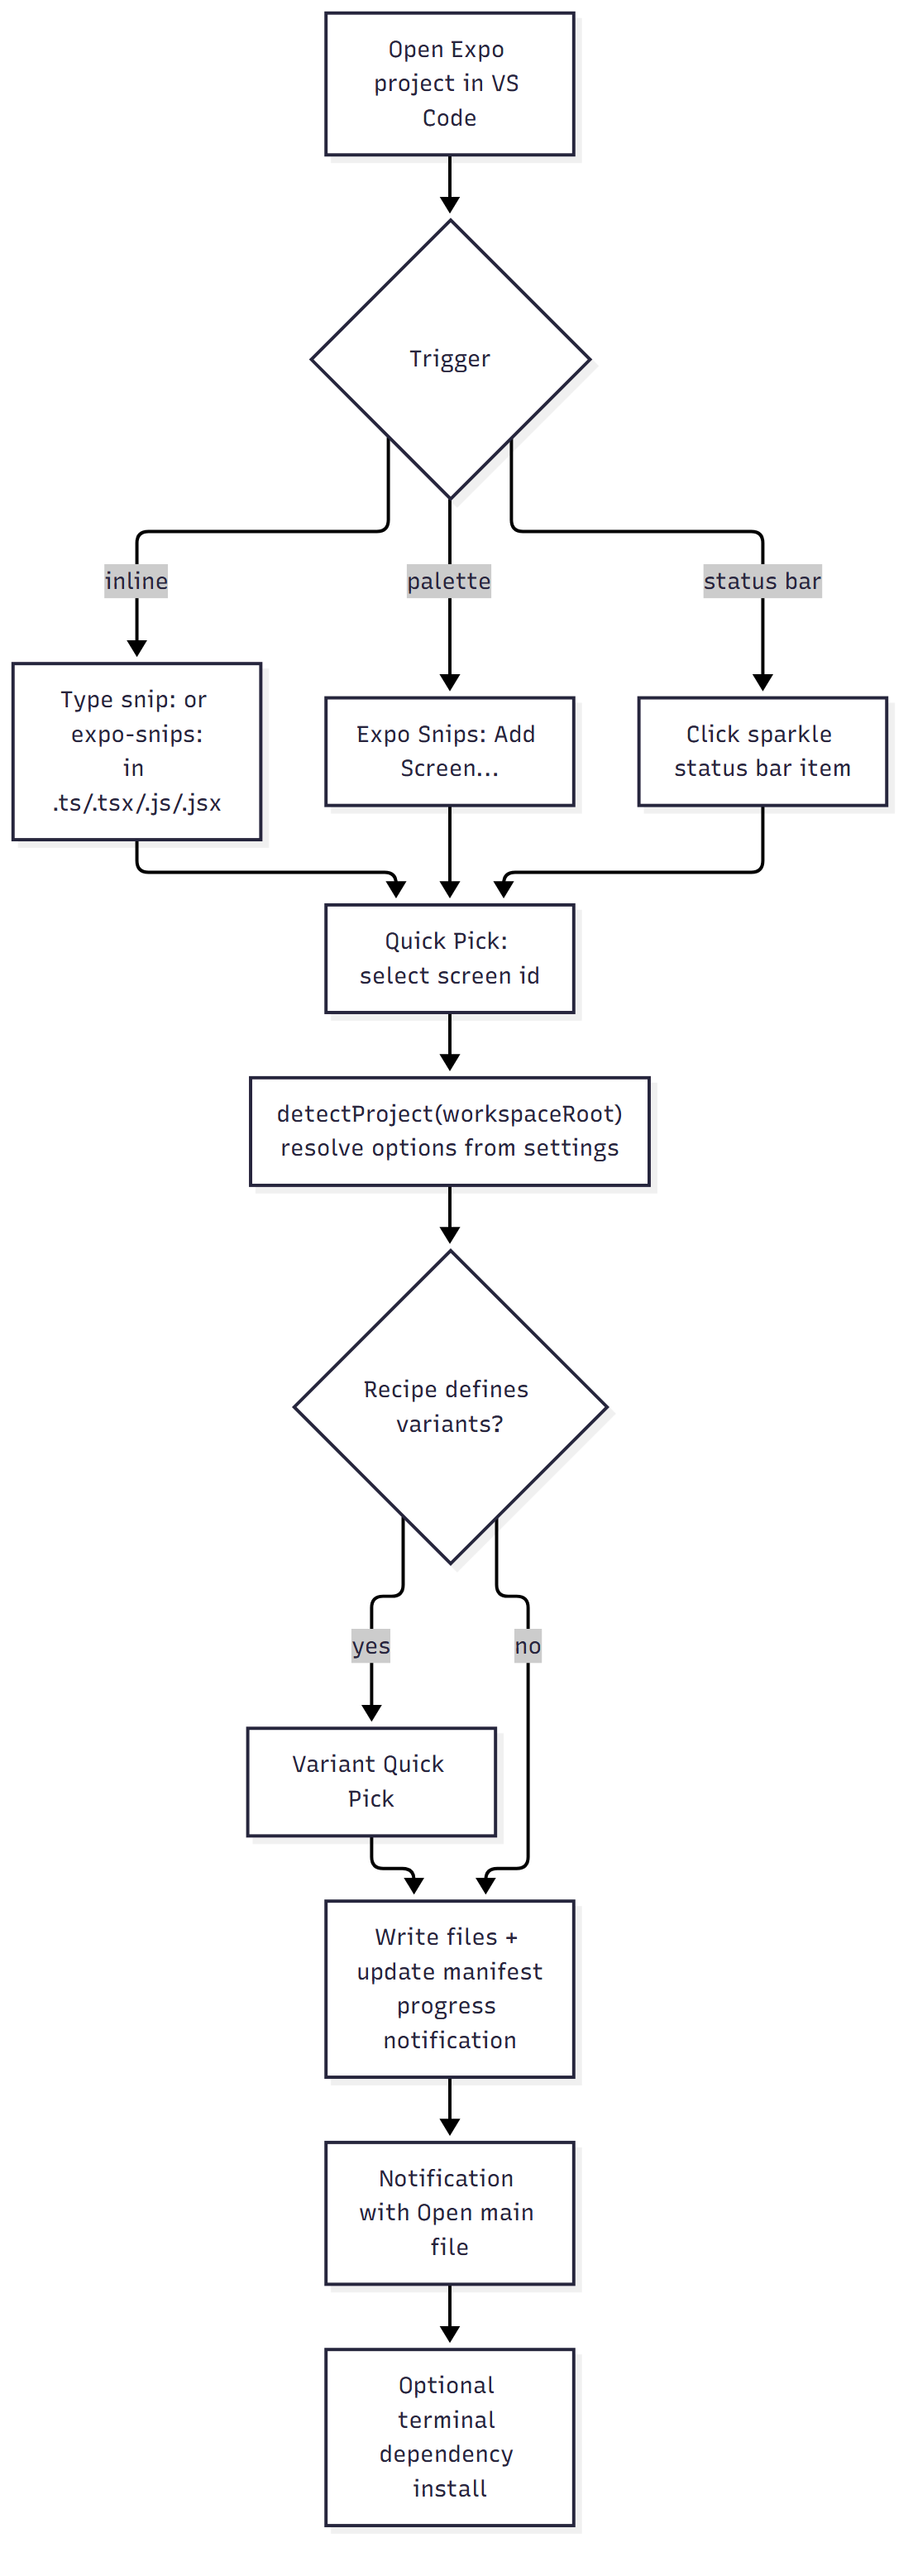
\includegraphics[width=0.9\textwidth]{diagrams/user-flow-vscode.png}
\caption{VS Code journey using the inline completion trigger}
\label{fig:user-flow-vscode-ux}
\end{figure}

\begin{longtable}{p{1cm}p{4.2cm}p{9.2cm}}
\caption{VS Code journey steps}\\
\toprule
\textbf{\#} & \textbf{Step} & \textbf{Detail} \\
\midrule

1 & Open a project & The extension activates on a TS/JS language or the command. \\
2 & Trigger & Type \texttt{snip:} or \texttt{expo-snips:}; or run ``Expo Snips: Add
Screen...''; or click the status bar item. \\
3 & Select & A Quick Pick lists recipe names with ids and descriptions. \\
4 & Resolve & Options are computed silently from detection and settings; a variant
Quick Pick appears only when the recipe declares variants. \\
5 & Generate & Files are written under a progress notification. \\
6 & Complete & An information message reports the file count and offers ``Open main
file''. \\
7 & Install & Dependencies are installed in an ``Expo Snips'' terminal when the
setting is enabled. \\
\bottomrule
\end{longtable}

\section{Variant selection flow}

\begin{enumerate}
  \item The CLI accepts \texttt{--variant glass}. For a recipe without a glass
        variant, the flag is accepted and the default template is used.
  \item In VS Code, \texttt{pickVariant} returns undefined when
        \texttt{recipe.variants} is empty; otherwise it shows a Quick Pick of
        variant labels and returns the selected id.
  \item During rendering, \texttt{resolveTemplateString} prefers the variant
        template over the default for that file entry.
\end{enumerate}

Only \texttt{app/home}, \texttt{auth/login} and \texttt{onboarding/welcome} define
variants, so the variant Quick Pick appears only for those three recipes.

\section{Update flow}

The update flow is documented as a state machine in Chapter~\ref{ch:data-flows}
(Figure~\ref{fig:update-flow}).

\section{Error and recovery flows}

\begin{longtable}{p{4.2cm}p{5cm}p{5.2cm}}
\caption{Recovery flows}\\
\toprule
\textbf{Situation} & \textbf{What the user sees} & \textbf{Recovery} \\
\midrule

Typo in screen id & ``Screen not found: <id>'' and a pointer to \texttt{list}. & Run
\texttt{list} and retry. \\
Unsupported option & ``Recipe "..." does not support <option> "...".'' & Omit the
flag; the tool will detect or prompt. \\
No files matched & ``No files matched the selected options. Nothing generated.'' &
Choose an option combination the recipe supports (check \texttt{list} output or
the recipe document). \\
Registry unreachable & CLI warning: ``Could not reach registry at <base>. Using N
built-in screens.'' & Remove or correct the registry base; generation continues
from the embedded catalog. \\
Option cancelled mid-prompt & Silent exit with code 1. & Re-run and complete the
prompts. \\
Update declined & ``Update cancelled.'' & Re-run when ready; nothing was written. \\
No manifest & ``No screens tracked in this project yet.'' & Run \texttt{add} first. \\
\bottomrule
\end{longtable}

\chapter{Data Flows}
\label{ch:data-flows}

\section{Principal data flow: generation}

\begin{figure}[H]
\centering
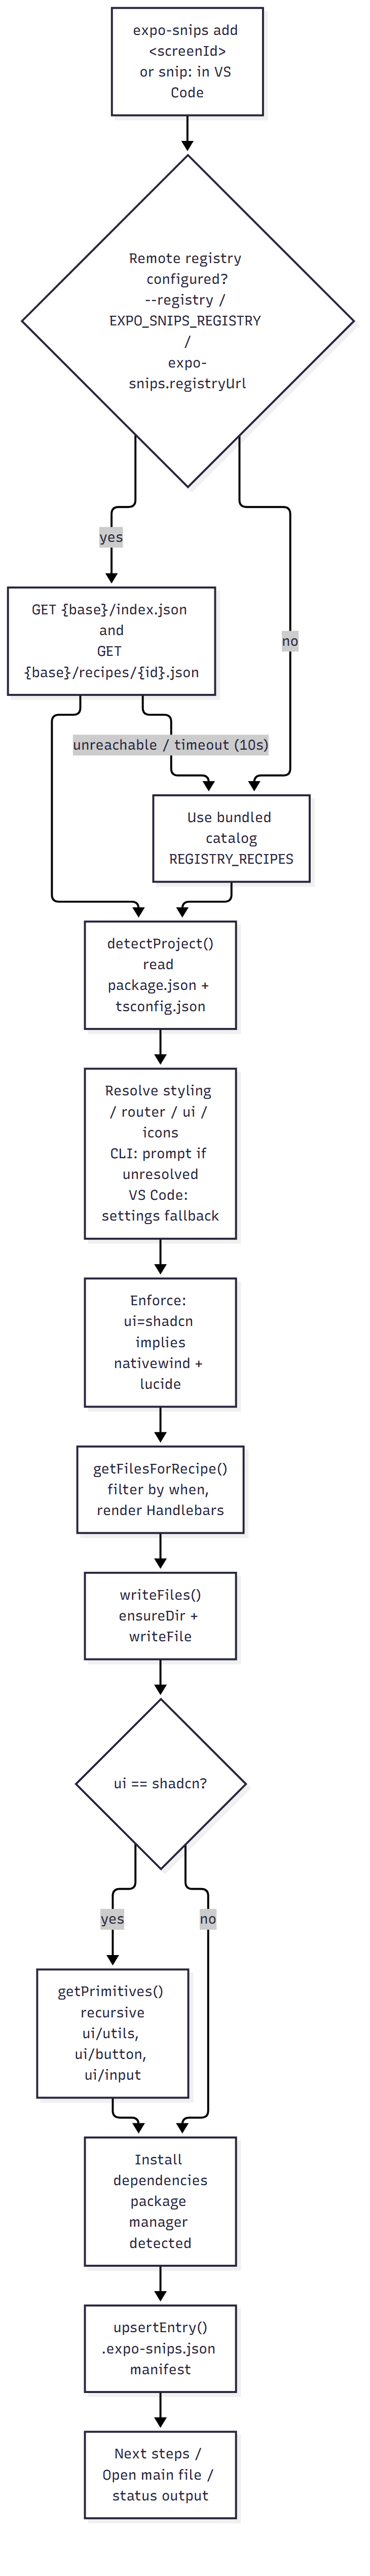
\includegraphics[width=\textwidth]{diagrams/generation-pipeline.png}
\caption{Generation data flow: from command input to persisted manifest}
\label{fig:data-flow-generation}
\end{figure}

\subsection*{Data transformations}

\begin{longtable}{p{3.4cm}p{4.4cm}p{6.6cm}}
\caption{Data transformations in the generation flow}\\
\toprule
\textbf{Input} & \textbf{Transformation} & \textbf{Output} \\
\midrule

Registry base string & \texttt{trim()} then strip trailing \texttt{/} & Normalised base \\
Index JSON array & Map to \texttt{RecipeIndexEntry[]} & Browsable index \\
Recipe JSON & Object with \texttt{files[].template} strings & \texttt{ScreenRecipe} \\
\texttt{package.json} + \texttt{tsconfig.json} & Four dependency probes + one file
probe & \texttt{DetectedProject} \\
Flags + detection + recipe \texttt{supported} & Precedence rules, prompts,
shadcn enforcement & \texttt{GenerationOptions} \\
\texttt{GenerationOptions} + variant & \texttt{buildRenderContext} & \texttt{RenderContext} \\
Recipe + context & \texttt{when} filter, template selection, Handlebars compile and
execute & \texttt{\{path, content\}[]} \\
File list + project root & \texttt{ensureDir} + \texttt{writeFile} & Files on disk \\
Recipe metadata & \texttt{upsertEntry} & Manifest entry \\
\bottomrule
\end{longtable}

\section{Registry resolution flow}

\begin{figure}[H]
\centering
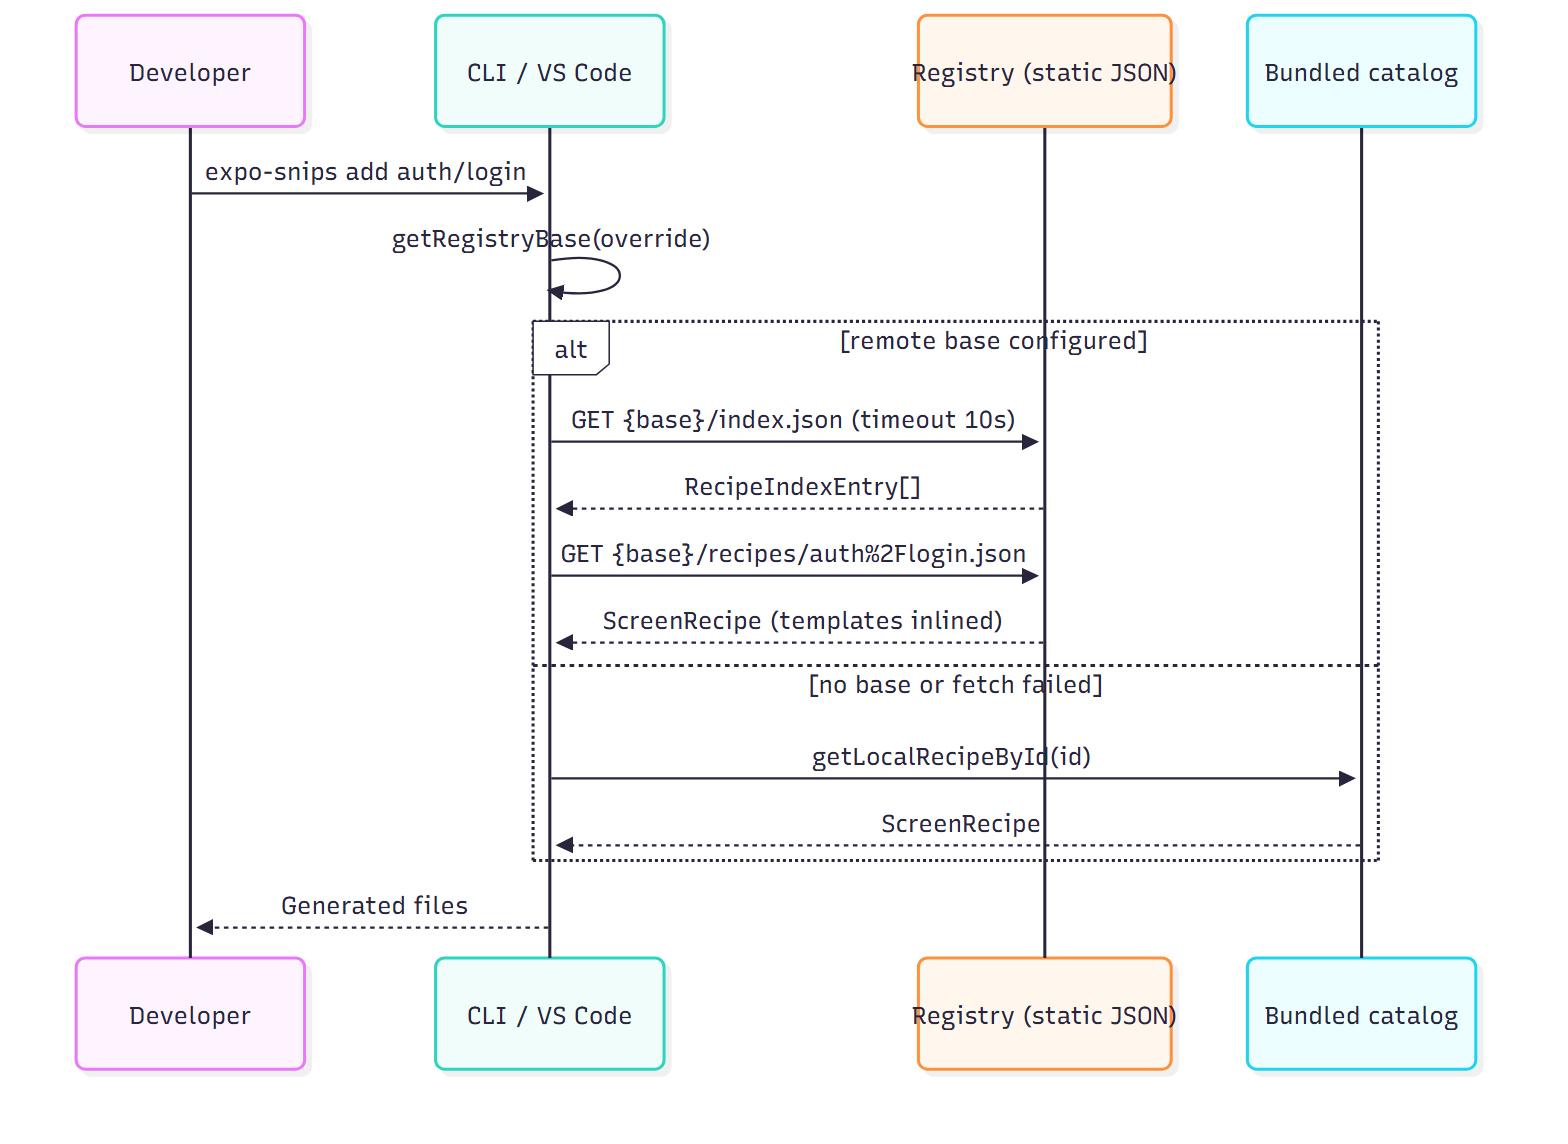
\includegraphics[width=0.94\textwidth]{diagrams/registry-api-sequence.png}
\caption{Sequence for resolving a recipe, including fallback}
\label{fig:data-flow-registry}
\end{figure}

\section{Primitive resolution flow}

\begin{figure}[H]
\centering
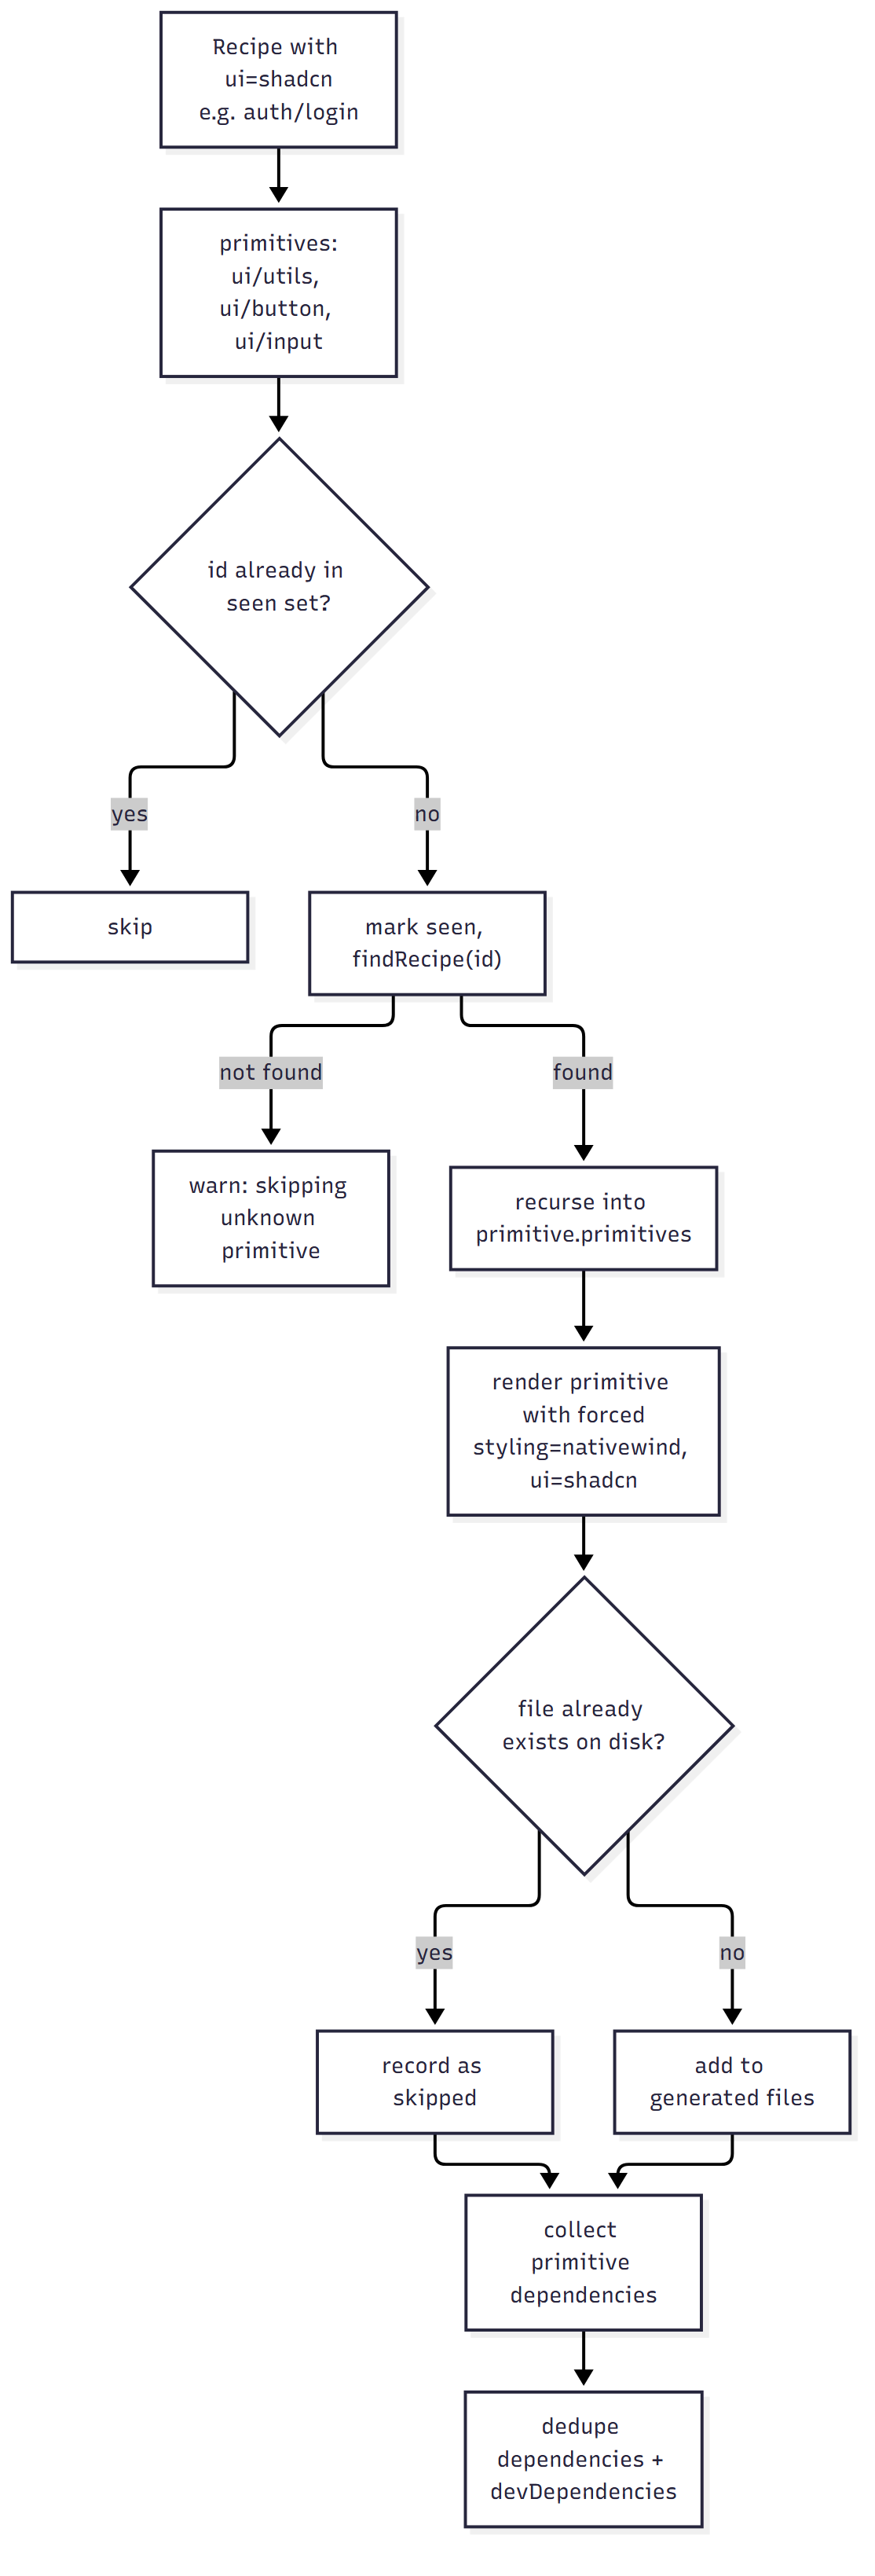
\includegraphics[width=0.95\textwidth]{diagrams/primitive-resolution.png}
\caption{Recursive primitive resolution data flow}
\label{fig:data-flow-primitives}
\end{figure}

The recursion is the only graph traversal in the codebase. It is guarded by a
\texttt{Set<string>} of seen ids, which makes the traversal terminate even if a
primitive cycle were introduced. Files whose paths already exist are excluded from
the generated set and reported as skipped.

\section{Update flow}

\begin{figure}[H]
\centering
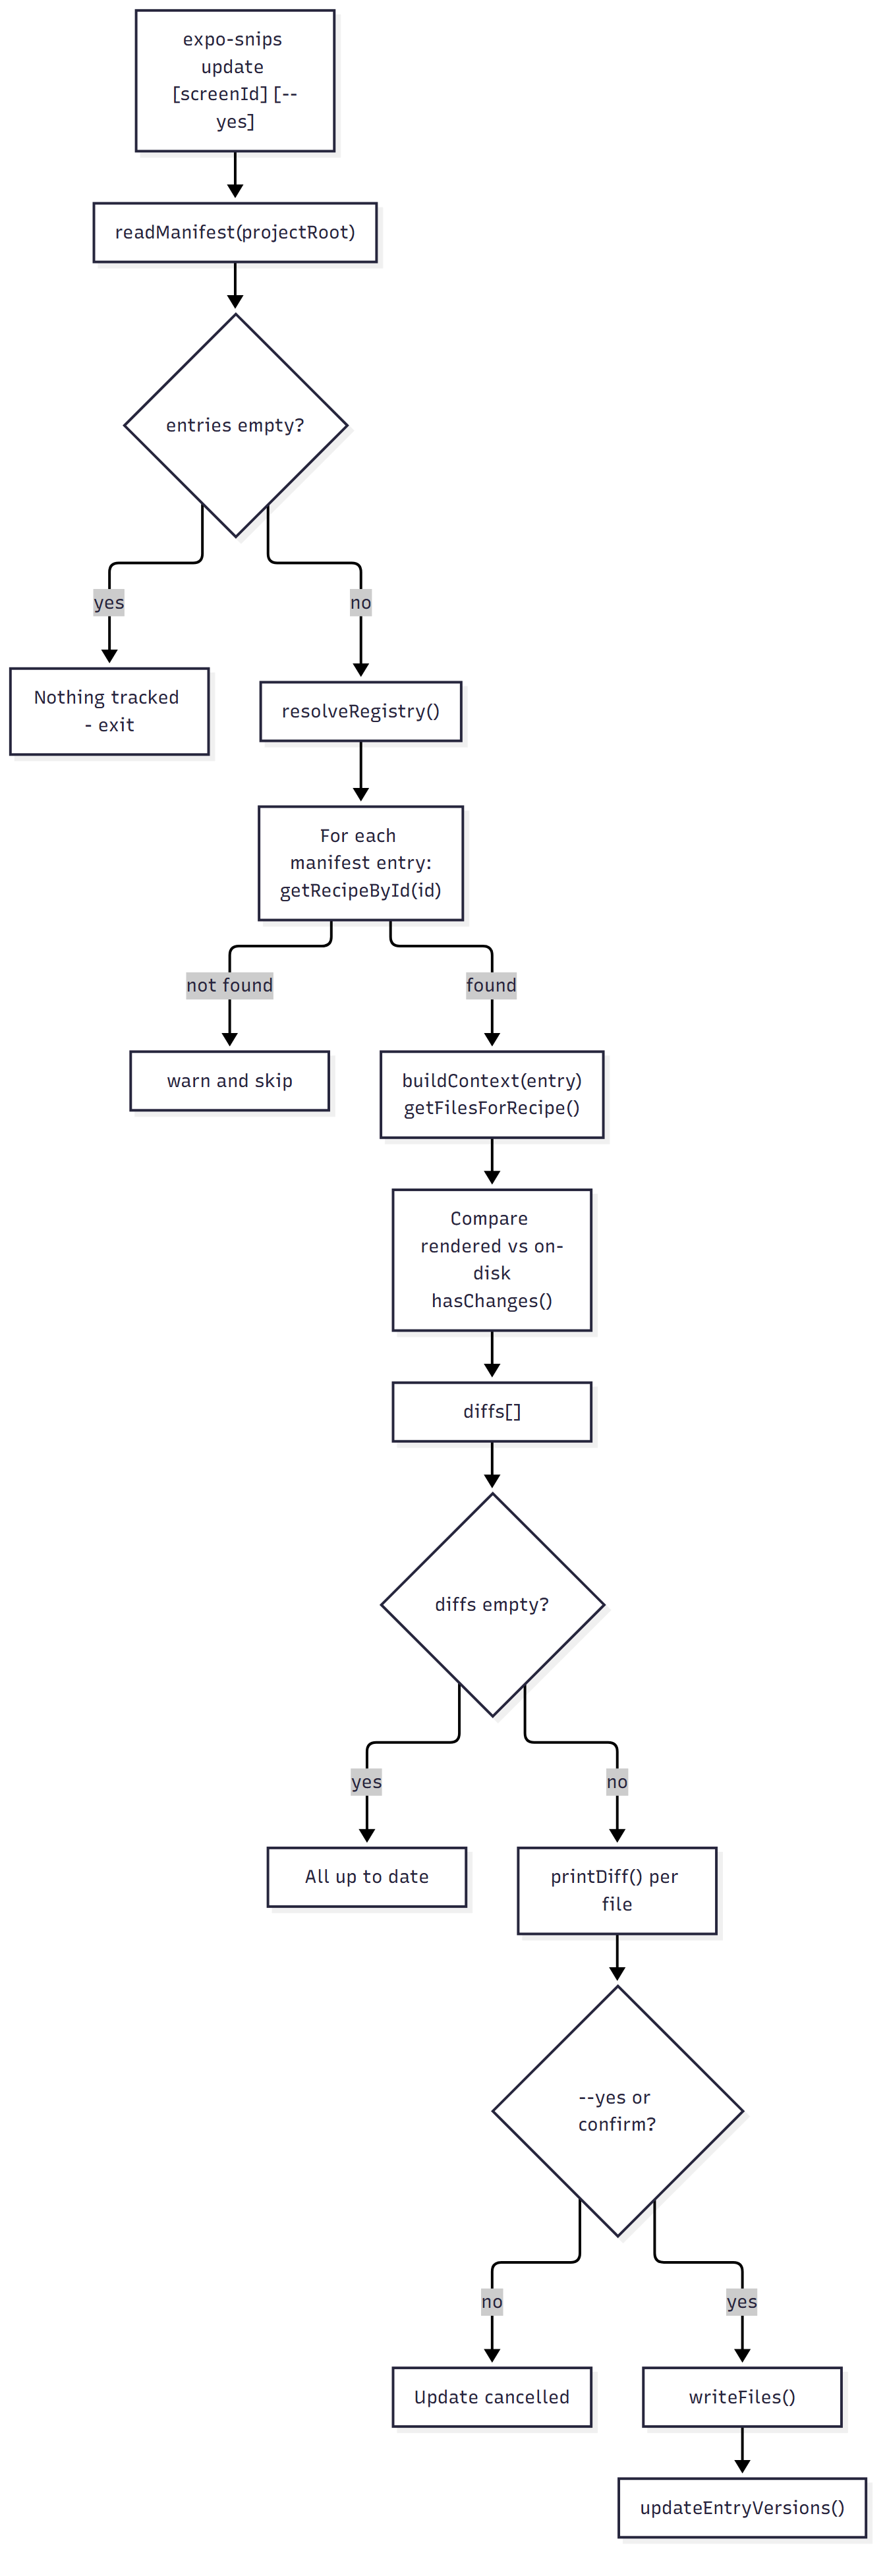
\includegraphics[width=0.95\textwidth]{diagrams/update-flow.png}
\caption{Update flow with diff preview and confirmation}
\label{fig:update-flow}
\end{figure}

\subsection*{Diff data structure}

\begin{lstlisting}[language=JavaScript]
interface DiffHunk { type: "add" | "remove" | "context"; line: string; }
\end{lstlisting}

\texttt{diffLines} builds an $(n+1) \times (m+1)$ dynamic-programming table over the
two line arrays (where $n$ and $m$ are the line counts) and walks it to emit hunks.
The algorithm is the classic longest-common-subsequence diff; it has no
line-number tracking, no hunk grouping and no context limit, so a large file change
prints every line. Colours: green for additions, red for removals, grey for
context.

\section{Migration and data at rest}

\begin{itemize}
  \item \textbf{Migrations:} \textbf{NOT APPLICABLE}. There is no database and no
        schema migration system.
  \item \textbf{Data at rest (1):} \texttt{.expo-snips.json} in the user's project.
        Written with two-space indentation; unreadable content is treated as an
        empty manifest rather than an error.
  \item \textbf{Data at rest (2):} the generated screen files themselves.
  \item \textbf{Data at rest (3):} the repository's own built registry
        (\texttt{registry/}) and the offline bundles.
  \item \textbf{Data in transit:} HTTP GET of JSON documents. No data leaves the
        user's machine except the request itself; no telemetry exists.
\end{itemize}

\section{Manifest lifecycle}

\begin{longtable}{p{3.2cm}p{4.2cm}p{7cm}}
\caption{Manifest lifecycle events}\\
\toprule
\textbf{Event} & \textbf{Operation} & \textbf{Effect} \\
\midrule

First generation & \texttt{upsertEntry} & File created with \texttt{version: 1} and one
entry. \\
Regeneration of the same recipe and variant & \texttt{upsertEntry} & Entry replaced
with fresh options, files, version and timestamp. \\
Generation of the same recipe with a different variant & \texttt{upsertEntry} &
A second, distinct entry is added (the upsert key includes the variant). \\
Update applied & \texttt{updateEntryVersions} & Matching entries receive the new
\texttt{recipeVersion}; \texttt{installedAt} and \texttt{options} are unchanged. \\
Manifest deleted & --- & The tool treats the project as having no tracked screens. \\
\bottomrule
\end{longtable}

\section{Data volumes}

\begin{table}[H]
\centering
\caption{Typical data volumes (measured from the repository)}
\begin{tabular}{p{5cm}p{9.2cm}}
\toprule
\textbf{Artefact} & \textbf{Size} \\
\midrule
Catalog index & 686 lines for 24 entries (mostly the \texttt{supported} objects). \\
Single built recipe & The \texttt{auth/login} recipe is the largest, with 7 file entries and inlined templates. \\
Full offline bundle & \texttt{packages/registry/bundle.json} is 242{,}775 bytes for 24 recipes. \\
Templates & 48 \texttt{.hbs} files. \\
Generated output per recipe & 1--7 files, each typically under 300 lines. \\
\bottomrule
\end{tabular}
\end{table}


% ---------------------------------------------------------------------
%  Part V: Experience and design system
% ---------------------------------------------------------------------
\chapter{UI / UX}
\label{ch:ui-ux}

Two distinct experiences must be described: the experience of the \emph{tool}
(terminal and editor) and the experience of the \emph{generated screens}.

\section{Tool experience --- terminal}

\begin{longtable}{p{4cm}p{10.2cm}}
\caption{Terminal interaction design}\\
\toprule
\textbf{Element} & \textbf{Design} \\
\midrule

Colour semantics & Cyan for informational headings
(\texttt{Generating "Login Screen" (auth/login)...}), green for success
(\texttt{\checkmark Login Screen added successfully!}), yellow for warnings and
notices, red for errors, dim grey for secondary detail (the effective options line,
the registry source line, skipped files). \\
Progressive disclosure & Options are asked for only when they cannot be resolved. \\
Defaults & Prompts preselect the detected value when the recipe supports it. \\
Filtering & Prompts list only the values the recipe supports. \\
Confirmation & The effective option set is printed before generation:
\texttt{styling=... router=... ui=... icons=... typescript=...}. \\
Per-file feedback & Each written file is announced as \texttt{Created
<path>}. \\
Follow-up guidance & Three concrete next steps after generation. \\
Safe abort & Any handled error leaves the exit code at 1 and writes nothing further. \\
\bottomrule
\end{longtable}

\section{Tool experience --- VS Code}

\begin{longtable}{p{4cm}p{10.2cm}}
\caption{Editor interaction design}\\
\toprule
\textbf{Element} & \textbf{Design} \\
\midrule

Discoverability & Three entry points (completion, command palette, status bar) so the
tool is reachable without reading documentation. \\
Inline trigger & The trigger regex matches only immediately before the cursor
(\texttt{snip:} or \texttt{expo-snips:}), so ordinary typing does not spam the
completion list. \\
Completion items & Labelled with the recipe id (the thing the user must type),
detailed with the display name, documented with the description and tags, sorted by
id. \\
Non-destructive insert & The completion inserts no text; selecting it runs the
generation command instead. This avoids leaving stray trigger text in the file. \\
Selection & Quick Pick matches on label and description
(\texttt{matchOnDescription: true}). \\
Progress & A progress notification covers the write phase. \\
Completion feedback & An information message reports the recipe name and file count,
and the message detail lists every generated path. \\
Follow-up action & A single ``Open main file'' button keeps the next step one click
away. \\
Empty catalog & A dedicated error message with an ``Open Settings'' action that
deep-links to the \texttt{expo-snips.registryUrl} setting. \\
\bottomrule
\end{longtable}

\section{Generated screen experience}

The generated screens share a consistent interaction vocabulary. The following is
observed across the templates.

\subsection*{States}

\begin{longtable}{p{4cm}p{10.2cm}}
\caption{States provided by generated screens}\\
\toprule
\textbf{State} & \textbf{Where and how} \\
\midrule

Loading & \texttt{isLoading} in \texttt{useLogin}/\texttt{useRegister}; a
\texttt{ActivityIndicator} is rendered in the native form. \\
Validation error & Per-field error text under the input, from
\texttt{formState.errors}. \\
Submission error & \texttt{error} state returned by the auth hooks plus
\texttt{Alert.alert}. \\
Empty & \texttt{utility/empty} --- icon, message and a primary action. \\
Error / retry & \texttt{utility/error} --- warning icon, message and a retry action. \\
Refresh & \texttt{app/home} wires a \texttt{RefreshControl} (its handler logs
\texttt{'refresh'}). \\
Unread indicator & \texttt{app/notifications} distinguishes read/unread and offers a
mark-all-read action. \\
Selected / unselected & \texttt{onboarding/features} cards and
\texttt{ecommerce} product cards. \\
\bottomrule
\end{longtable}

\subsection*{Input and validation patterns}

\begin{itemize}
  \item Controlled inputs through \texttt{react-hook-form}'s \texttt{Controller}.
  \item Email fields set \texttt{keyboardType="email-address"} and
        \texttt{autoCapitalize="none"}.
  \item Password fields combine a secure entry toggle with
        \texttt{secureTextEntry}.
  \item The OTP recipe uses a segmented input with auto-advance and auto-submit on
        completion and an error message plus a resend affordance.
  \item Labels are rendered above the field in the native variant; the shadcn
        variant instead pairs an icon with a borderless input inside a row.
\end{itemize}

\subsection*{Navigation patterns}

\begin{itemize}
  \item Expo Router screens use \texttt{Link} with route strings
        (\texttt{/register}, \texttt{/forgot-password}, \texttt{/}).
  \item The react-navigation login and register screens use
        \texttt{useNavigation()} and \texttt{navigation.goBack()}.
  \item Back affordances are a left chevron or an arrow-left icon inside a
        pressable, consistent with the surrounding palette.
\end{itemize}

\section{Responsive design}

All layouts use flex containers and percentage/flex sizing rather than fixed
widths, so they adapt to phone and tablet. Concrete evidence:

\begin{itemize}
  \item \texttt{ecommerce/products} uses a two-column \texttt{FlatList} grid.
  \item \texttt{app/home} uses \texttt{flex-1} stat cards in a row.
  \item Forms are wrapped in a \texttt{ScrollView} with
        \texttt{keyboardShouldPersistTaps="handled"} and a
        \texttt{KeyboardAvoidingView} whose behaviour switches on platform
        (\texttt{padding} on iOS, \texttt{height} on Android).
  \item Lists use \texttt{react-native-safe-area-context}'s \texttt{SafeAreaView}
        in some templates and React Native's own \texttt{SafeAreaView} in others ---
        an inconsistency recorded in Chapter~\ref{ch:technical-debt}.
\end{itemize}

\section{Animations and interaction feedback}

\begin{itemize}
  \item The use of \texttt{Pressable} provides the platform's native press
        feedback.
  \item The shadcn-style \texttt{Button} adds opacity changes on press
        (\texttt{active:opacity-90}) and web-only hover/focus ring behaviour.
  \item No template uses \texttt{Animated}, \texttt{Reanimated},
        \texttt{Moti} or layout transitions.
\end{itemize}

\textbf{Status:} IMPLEMENTED (as an observed absence of animation).

\section{Accessibility}

\textbf{Finding.} No generated template sets
\texttt{accessibilityLabel}, \texttt{accessibilityRole},
\texttt{accessibilityHint} or \texttt{accessibilityState}. Interactive elements are
\texttt{Pressable}s and \texttt{TextInput}s without labels for assistive
technology. Icon-only buttons (for example the header bell, search and back
buttons) expose no text alternative.

\begin{longtable}{p{1.4cm}p{4.4cm}p{3cm}p{5.4cm}}
\caption{Accessibility finding}\\
\toprule
\textbf{ID} & \textbf{Finding} & \textbf{Severity} & \textbf{Evidence} \\
\midrule

A11Y-01 & Icon-only pressables have no accessibility label. & Medium & Every template with an icon button, e.g. \texttt{app/home} header actions. \\
A11Y-02 & No accessibility roles or hints are declared anywhere. & Medium & Repo-wide absence across 48 templates. \\
A11Y-03 & Form error text is not associated with its input for assistive technology. & Medium & \texttt{components.login-form.hbs} renders errors as sibling \texttt{Text}. \\
A11Y-04 & Colour contrast of the glass variant (\texttt{\#0F172A} surface with white text) is good; the muted greys (\texttt{\#9CA3AF}) on white are below WCAG AA for body text. & Low & \texttt{\#9CA3AF} used for timestamps and placeholders. \\
\bottomrule
\end{longtable}

\textbf{Status:} RECOMMENDED (add accessibility props and confirm contrast ratios).

\section{Dark mode}

Only the \texttt{glass} variant is effectively dark
(\texttt{\#0F172A}); there is no theme switch, no \texttt{useColorScheme}
integration and no light/dark token set. Screens are light-themed otherwise.

\textbf{Status:} IMPLEMENTED (light only) / RECOMMENDED (theming support).

\chapter{Design System}
\label{ch:design-system}

\section{Scope}

Expo Snips ships design decisions in the form of generated screens rather than as a
documented design system. This chapter extracts the system that is actually encoded
in the 48 Handlebars templates. Every value below is a literal found in
\texttt{packages/registry/templates/**/*.hbs}.

\textbf{Status:} IMPLEMENTED (values) / INFERRED (organisation into a system).

\section{Colour palette}

The generated screens use a Tailwind-derived, light, neutral palette with a blue
accent. Counts are the number of occurrences across all templates.

\begin{longtable}{p{2.3cm}p{2.2cm}p{1.7cm}p{1.2cm}p{5.8cm}}
\caption{Colour palette derived from template literals}\\
\toprule
\textbf{Hex} & \textbf{Tailwind} & \textbf{Count} & \textbf{Role} & \textbf{Usage} \\
\midrule

\texttt{\#2563EB} & blue-600 & 40 & Primary & Accent links, active states, primary
buttons, check marks, key icons. \\
\texttt{\#FFFFFF} & white & 74 & Surface & Cards, inputs, icon buttons, sheets. \\
\texttt{\#F9FAFB} & gray-50 & 10 & Canvas & App background behind cards. \\
\texttt{\#F3F4F6} & gray-100 & 16 & Divider & List separators, chart placeholders. \\
\texttt{\#E5E7EB} & gray-200 & 2 & Border & Secondary borders. \\
\texttt{\#D1D5DB} & gray-300 & 7 & Border & Input and checkbox borders. \\
\texttt{\#9CA3AF} & gray-400 & 28 & Muted text & Timestamps, placeholders, chevrons. \\
\texttt{\#6B7280} & gray-500 & 45 & Secondary text & Body copy, labels, secondary icons. \\
\texttt{\#4B5563} & gray-600 & 19 & Icon & Default icon colour. \\
\texttt{\#374151} & gray-700 & 18 & Strong body & Article body, menu labels. \\
\texttt{\#111827} & gray-900 & 65 & Primary text & Headings and titles. \\
\texttt{\#EFF6FF} & blue-50 & 5 & Tint & Selected rows, light blue fills. \\
\texttt{\#DBEAFE} & blue-100 & 3 & Tint & Avatar placeholder background. \\
\texttt{\#BFDBFE} & blue-200 & 1 & Tint & Product placeholder block. \\
\texttt{\#93C5FD} & blue-300 & 3 & Accent & Decorative accents. \\
\texttt{\#60A5FA} & blue-400 & 7 & Accent & Chart bars, highlights. \\
\texttt{\#3B82F6} & blue-500 & 1 & Accent & Scheduled event colour. \\
\texttt{\#0F172A} & slate-900 & 3 & Dark surface & Glass-variant background only. \\
\texttt{\#10B981} & emerald-500 & 4 & Success & Positive trend indicators. \\
\texttt{\#16A34A} & green-600 & 1 & Success & Success status. \\
\texttt{\#15803D} & green-700 & 1 & Success text & Success copy. \\
\texttt{\#D1FAE5} & emerald-100 & 1 & Success fill & Success background. \\
\texttt{\#DCFCE7} & green-100 & 1 & Success fill & Success background. \\
\texttt{\#F0FDF4} & green-50 & 1 & Success fill & Success background. \\
\texttt{\#F59E0B} & amber-500 & 9 & Rating / warning & Star ratings. \\
\texttt{\#FEF3C7} & amber-100 & 1 & Warning fill & Warning background. \\
\texttt{\#EF4444} & red-500 & 21 & Error & Error text, destructive icons, negative
trends. \\
\texttt{\#DC2626} & red-600 & 1 & Error text & Destructive action label. \\
\texttt{\#FEE2E2} & red-100 & 1 & Error fill & Error background. \\
\texttt{\#FEF2F2} & red-50 & 1 & Error fill & Error surface. \\
\texttt{\#8B5CF6} & violet-500 & 2 & Data accent & Secondary chart series and event
colour. \\
\texttt{\#E0E7FF} & indigo-100 & 1 & Data accent & Placeholder block. \\
\texttt{\#FCE7F3} & pink-100 & 1 & Data accent & Placeholder block. \\
\bottomrule
\end{longtable}

\subsection*{Semantic mapping (recommended)}

For a future brand or product site, the following mapping is consistent with the
templates' own usage. \textbf{Status:} RECOMMENDED.

\begin{table}[H]
\centering
\caption{Recommended semantic colour mapping}
\begin{tabular}{p{4cm}p{2.6cm}p{7.4cm}}
\toprule
\textbf{Role} & \textbf{Value} & \textbf{Tokens observed in templates} \\
\midrule
Primary / accent & \texttt{\#2563EB} & \texttt{bg-primary}, \texttt{text-primary} \\
Primary on accent & \texttt{\#FFFFFF} & \texttt{text-primary-foreground} \\
Canvas & \texttt{\#F9FAFB} & \texttt{bg-gray-50} \\
Surface & \texttt{\#FFFFFF} & \texttt{bg-white}, \texttt{bg-background} \\
Text primary & \texttt{\#111827} & \texttt{text-gray-900}, \texttt{text-foreground} \\
Text secondary & \texttt{\#6B7280} & \texttt{text-gray-500}, \texttt{text-muted-foreground} \\
Border & \texttt{\#D1D5DB} & \texttt{border-input}, \texttt{border-gray-300} \\
Destructive & \texttt{\#EF4444} & \texttt{bg-destructive}, \texttt{text-destructive} \\
Success & \texttt{\#10B981} & trend indicators \\
Warning & \texttt{\#F59E0B} & rating stars \\
\bottomrule
\end{tabular}
\end{table}

\section{shadcn-style design tokens}

When \texttt{ui=shadcn} is selected, templates switch from literal colour values to
semantic utility tokens. The tokens actually referenced in templates are:

\begin{table}[H]
\centering
\caption{Tokens referenced by shadcn-style templates}
\begin{tabular}{p{4.4cm}p{9.4cm}}
\toprule
\textbf{Token} & \textbf{Where used} \\
\midrule
\texttt{bg-background}, \texttt{text-foreground} & Screen containers and titles in
\ttfamily app.*.index.shadcn.hbs \\
\texttt{text-muted-foreground} & Subtitles and secondary text \\
\texttt{text-destructive} & Validation error messages \\
\texttt{bg-primary}, \texttt{text-primary-foreground} & Default button variant \\
\texttt{bg-primary/10} & Selected OTP cell fill \\
\texttt{border-input} & Input and outline-button borders \\
\texttt{bg-secondary}, \texttt{text-secondary-foreground} & Secondary button variant \\
\texttt{bg-accent}, \texttt{text-accent-foreground} & Outline/ghost hover states \\
\texttt{ring-ring} & Web focus ring on buttons \\
\texttt{rounded-md} (inputs, buttons) & Control radius \\
\bottomrule
\end{tabular}
\end{table}

\textbf{Important gap.} No Tailwind or NativeWind theme configuration is present in
the repository (\texttt{no tailwind.config.*} or NativeWind theme file exists).
The tokens above require such a configuration to resolve to concrete colours. This
is recorded as a known issue and a high-priority technical-debt item
(Chapters~\ref{ch:known-issues} and~\ref{ch:technical-debt}).

\section{Typography}

\begin{itemize}
  \item \textbf{Font family:} none is specified. All templates inherit the React
        Native platform default (system font). No \texttt{fontFamily} appears in any
        template.
  \item \textbf{Weights:} \texttt{font-bold} for titles and statistic values,
        \texttt{font-medium} for labels and button text, regular for body copy.
\end{itemize}

\begin{table}[H]
\centering
\caption{Type scale (Frontend)}
\begin{tabular}{p{3.2cm}p{2.2cm}p{2.2cm}p{6.2cm}}
\toprule
\textbf{Style} & \textbf{Class} & \textbf{px} & \textbf{Use} \\
\midrule
Page title & \texttt{text-3xl} & 30 & Auth and onboarding headings (shadcn variant) \\
Page title & \texttt{text-2xl} & 24 & Home greeting, header titles \\
Section title & \texttt{text-lg} & 18 & Section headings, card titles \\
Body & \texttt{text-base} & 16 & Form values, list titles \\
Body small & \texttt{text-sm} & 14 & Labels, secondary copy, buttons \\
Meta & \texttt{text-xs} & 12 & Timestamps, deltas, captions \\
\bottomrule
\end{tabular}
\end{table}

StyleSheet variants encode the same scale numerically (\texttt{fontSize: 12, 14,
16, 18, 24}) with the same weight conventions.

\section{Spacing}

Spacing is a multiple-of-four scale, expressed either as utility classes or as
numeric StyleSheet values.

\begin{table}[H]
\centering
\caption{Spacing scale observed in templates}
\begin{tabular}{p{3cm}p{2.6cm}p{8.2cm}}
\toprule
\textbf{Value (px)} & \textbf{Class} & \textbf{Typical use} \\
\midrule
4 & \texttt{gap-1}, \texttt{mt-1} & Label-to-error spacing \\
8 & \texttt{gap-2}, \texttt{mb-2} & Icon-to-text gaps \\
12 & \texttt{gap-3}, \texttt{ml-3} & List item internal spacing \\
16 & \texttt{gap-4}, \texttt{p-4} & Card padding, form field gaps \\
20 & \texttt{px-5} & Screen horizontal padding \\
24 & \texttt{p-6}, \texttt{mt-6} & Section separation, screen padding \\
32 & \texttt{mt-8} & Major section separation \\
\bottomrule
\end{tabular}
\end{table}

Screen padding is consistently 20\,px horizontally for list/dashboard screens and
24\,px for auth and onboarding screens.

\section{Border radius}

\begin{table}[H]
\centering
\caption{Radius scale}
\begin{tabular}{p{3.4cm}p{2.2cm}p{8.2cm}}
\toprule
\textbf{Class} & \textbf{px} & \textbf{Use} \\
\midrule
\texttt{rounded-2xl} & 16 & Cards, stat tiles, task rows \\
\texttt{rounded-xl} & 12 & Secondary containers \\
\texttt{rounded-lg} & 8 & Inputs and buttons (native variant) \\
\texttt{rounded-md} & 6 & Inputs and buttons (shadcn variant) \\
\texttt{rounded-full} & --- & Icon buttons (40$\times$40 with radius 20), avatars,
checkbox dots \\
\bottomrule
\end{tabular}
\end{table}

\section{Elevation, borders and shadows}

\begin{itemize}
  \item \textbf{No shadow or elevation properties appear in any template.} Depth is
        conveyed by white surfaces on a grey canvas rather than by shadows.
  \item Borders are used sparingly: \texttt{borderWidth: 2} for checkboxes and OTP
        cells, single-pixel top/bottom borders for list dividers
        (\texttt{\#F3F4F6}).
  \item The glass variant substitutes translucency
        (\texttt{rgba(255,255,255,0.08)}) for elevation.
\end{itemize}

\textbf{Status:} IMPLEMENTED (absence of shadows is verifiable).

\section{Component inventory}

\begin{longtable}{p{3.6cm}p{10.6cm}}
\caption{Design-system components demonstrated by recipes}\\
\toprule
\textbf{Component} & \textbf{Characteristic styling} \\
\midrule

Card & White, 16\,px radius, 16\,px padding. \\
Stat tile & Card with a small icon-plus-label row, a 24\,px bold value and a 12\,px
delta line. \\
Button (native) & Full-width pressable with an accent fill and white label. \\
Button (shadcn) & \texttt{cva}-driven variants: default, destructive, outline,
secondary, ghost, link; sizes default/sm/lg/icon; forwardRef wrapper around
\texttt{Pressable} with automatic \texttt{Text} child wrapping. \\
Input (native) & Label above field, bordered row, optional leading icon, error text
below. \\
Input (shadcn) & \texttt{TextInput} with tokenised classes, placeholder colour
\texttt{\#9ca3af}, native height override. \\
Icon button & 40$\times$40 circle, white, centred icon (20--24\,px). \\
OTP input & Segmented cells, selected cell tinted, auto-advance, auto-submit. \\
List row & Icon or avatar, title, subtitle, chevron or badge. \\
Search bar & Rounded input with a leading search icon. \\
Toggle row & Label plus a \texttt{Switch}, grouped in a white block with dividers. \\
Chip & Recent-search pill; category filter. \\
Rating & Amber star row with a numeric value. \\
Avatar & Circle with initials or a tinted background. \\
Bottom sheet & Location detail sheet over a map. \\
Empty state & Centred muted icon, title, message and a primary action. \\
\bottomrule
\end{longtable}

\section{Icons}

\begin{itemize}
  \item \textbf{Library:} \texttt{lucide-react-native}, declared as a dependency by
        almost every recipe.
  \item \textbf{Sizes:} 12--24\,px, with 16 and 20 most common; colour is set
        explicitly, usually \texttt{\#4B5563} for inactive icons, \texttt{\#9CA3AF}
        for chevrons and \texttt{\#2563EB} for active state.
  \item \textbf{Degradation:} template conditionals remove icon imports and icon
        elements entirely when \texttt{icons} is \texttt{none}, leaving text-only
        layouts.
\end{itemize}

\section{Breakpoints and responsive units}

There is no breakpoint system. Layouts are flex-based and therefore inherently
fluid. The only explicit responsiveness mechanism is NativeWind's \texttt{web:}
prefix, used in the shadcn primitives for web-only hover, focus and sizing
behaviour (for example \texttt{web:focus-visible:ring-2} and
\texttt{native:h-12}).

\section{Animation}

No template uses an animation library, transition or layout animation. Press
feedback is provided by the platform's \texttt{Pressable}. The button primitive
adds opacity transitions on press. This is the extent of the motion design.

\section{Design-system gap summary}

\begin{table}[H]
\centering
\caption{Design-system gaps}
\begin{tabular}{p{4.6cm}p{9.2cm}}
\toprule
\textbf{Gap} & \textbf{Detail} \\
\midrule
No theme configuration & shadcn tokens are referenced but no Tailwind/NativeWind
theme defines them. \\
No atomic primitives for the native path & Native-variant screens hand-roll inputs
and buttons instead of drawing on shared primitives. \\
No accessibility props & See Section~\ref{ch:ui-ux}. \\
No dark mode & Only the glass variant is dark, and it is a one-off template. \\
No icon abstraction & lucide icons are imported directly per template. \\
Spacing tokens not centralised & Values are repeated literally, not defined once. \\
\bottomrule
\end{tabular}
\end{table}

\textbf{Status:} IMPLEMENTED (gaps are verifiable) / RECOMMENDED (centralising the
system in a theme file).


% ---------------------------------------------------------------------
%  Part VI: Quality, security and operations
% ---------------------------------------------------------------------
\chapter{Security}
\label{ch:security}

\section{Method and scope}

The review covers the repository's own source, templates, build scripts and CI
configuration. Findings are stated in a fixed format: finding, severity, evidence,
impact and recommendation. Severity reflects impact in the product's real deployment
model --- a locally executed developer tool that writes files into the user's
project and may fetch content from a configurable registry.

\section{Secrets}

\begin{longtable}{p{1.3cm}p{3.4cm}p{1.9cm}p{6.1cm}p{1.5cm}}
\caption{Secret-related findings}\\
\toprule
\textbf{ID} & \textbf{Finding} & \textbf{Severity} & \textbf{Evidence} & \textbf{Status} \\
\midrule

SEC-01 & No secrets are committed. A recursive search for \texttt{.env} files found
none, and no credential literals appear in source, templates or workflows. & --- &
Absence verified across the tree. & PASS \\
SEC-02 & CI uses repository secrets for publishing
(\texttt{NPM\_TOKEN}) and the workflow default token
(\texttt{GITHUB\_TOKEN}), both referenced indirectly rather than inlined. &
--- & \texttt{publish.yml}, \texttt{deploy-registry.yml}. & PASS \\
SEC-03 & The CLI has no mechanism to store credentials; it therefore cannot leak
them. & --- & \texttt{registry.ts} performs unauthenticated GET only. & PASS \\
\bottomrule
\end{longtable}

\section{Injection}

\begin{longtable}{p{1.3cm}p{3.6cm}p{1.9cm}p{5.8cm}p{1.6cm}}
\caption{Injection findings}\\
\toprule
\textbf{ID} & \textbf{Finding} & \textbf{Severity} & \textbf{Evidence} & \textbf{Status} \\
\midrule

SEC-04 & \textbf{Shell command construction from unvalidated user input} in
\texttt{init}. The project name is interpolated directly into a shell string that
is executed with inherited stdio. A name containing shell metacharacters or quote
breakout would be interpreted by the shell. & High &
\texttt{packages/cli/src/commands/init.ts}, lines 20--23. & OPEN \\
SEC-05 & \textbf{Dependency names are interpolated into an executed shell
command.} Recipe \texttt{dependencies} strings are joined and passed to
\texttt{execSync}. With a bundled catalog this is trusted data; with a remote
registry, recipe content becomes an execution vector (see SEC-08). & High &
\texttt{packages/cli/src/utils/installDeps.ts}, lines 25 and 35. & OPEN \\
SEC-06 & No SQL, NoSQL or ORM access exists, so SQL injection is
\textbf{NOT APPLICABLE}. & --- & No database in the project. & N/A \\
SEC-07 & Template rendering is not a code-execution path: Handlebars is used in
default (non-helper-registering) mode with only the \texttt{eq} and \texttt{neq}
helpers added, and generated output is written to files rather than evaluated. & Low &
\texttt{packages/core/src/generate.ts}, lines 5--6. & ACCEPTED \\
\bottomrule
\end{longtable}

\subsection*{SEC-04 / SEC-05 --- details and recommendation}

\begin{lstlisting}[language=JavaScript]
// packages/cli/src/commands/init.ts (excerpt)
const nameArg = name ? `${name}` : ".";
const cmd = `npx create-expo-app@latest ${nameArg} --template ${template} --yes`;
execSync(cmd, { cwd: process.cwd(), stdio: "inherit" });
\end{lstlisting}

Both \texttt{name} and \texttt{template} come from argv. Neither is validated or
quoted.

\textbf{Impact:} a crafted project name (for example one containing
\texttt{;}, \texttt{\&\&} or a backtick) executes arbitrary commands with the user's
privileges. The risk is partly self-inflicted (the user types their own name), but
the command may also be supplied by a script, CI job or documentation snippet.

\textbf{Recommendation:} use \texttt{execFileSync} (or
\texttt{spawnSync}) with an argument array so no shell is involved, and validate
the project name against a conservative pattern
(\texttt{\^{}[A-Za-z0-9.\_-]+\$}). Apply the same treatment to the dependency
installer, and validate dependency strings against npm package-name grammar.

\section{Trust boundary: the registry}

\begin{longtable}{p{1.3cm}p{3.6cm}p{1.9cm}p{5.8cm}p{1.6cm}}
\caption{Remote-content findings}\\
\toprule
\textbf{ID} & \textbf{Finding} & \textbf{Severity} & \textbf{Evidence} & \textbf{Status} \\
\midrule

SEC-08 & \textbf{Remote recipes are rendered and written verbatim, with no
verification.} A configured registry can return any \texttt{files[].path} and any
template content; the client writes those paths into the user's project and
installs declared dependencies. & High &
\texttt{getRecipeById} (both clients) plus \texttt{writeFiles},
\texttt{installDeps}. & OPEN \\
SEC-09 & Path traversal is not validated on generated paths. A recipe path
containing \texttt{..} would resolve outside the project root because paths are
joined without containment checks. & High &
\texttt{writeFiles.ts} line 14; \texttt{generator.ts} line 215. & OPEN \\
SEC-10 & HTTPS is not enforced. A registry base of \texttt{http://} is accepted
without warning. & Medium & \texttt{getRegistryBase} accepts any string. & OPEN \\
SEC-11 & There is no integrity check (hash or signature) on fetched recipe
documents. & Medium & \texttt{fetchJSON} returns parsed JSON directly. & OPEN \\
\bottomrule
\end{longtable}

\textbf{Overall assessment.} Because the default configuration uses the embedded
catalog, the system is safe out of the box. The moment a remote registry is
configured --- which the product actively documents and supports --- the registry
becomes a trusted code-distribution channel with none of the controls a package
manager applies (no signature, no hash, no review, no path containment). This is
the single most important security consideration in the product.

\textbf{Recommendation (RECOMMENDED):}
\begin{itemize}
  \item reject or normalise any generated path that escapes the project root;
  \item validate dependency strings against the npm name grammar;
  \item warn or refuse when a non-HTTPS registry is configured;
  \item consider publishing a manifest of recipes with content hashes and
        verifying it client-side;
  \item document the trust implications of \texttt{--registry} prominently.
\end{itemize}

\section{Generated-code findings}

\begin{longtable}{p{1.3cm}p{3.6cm}p{1.9cm}p{5.8cm}p{1.6cm}}
\caption{Findings in generated screens}\\
\toprule
\textbf{ID} & \textbf{Finding} & \textbf{Severity} & \textbf{Evidence} & \textbf{Status} \\
\midrule

SEC-12 & \textbf{Credentials are logged to the console.} The generated login and
register hooks execute \texttt{console.log('Login attempt', \{ email, password
\})}, and the shadcn form logs the whole form payload. & Medium &
\texttt{hooks.use-login.hbs}; \texttt{components.login-form.shadcn.hbs}. & OPEN \\
SEC-13 & \textbf{Authentication is a placeholder.} Submission always succeeds after
a fixed delay and shows a success alert. If a developer ships without replacing it,
the app reports successful login for any credentials. & High &
\texttt{hooks.use-login.hbs}, \texttt{hooks.use-register.hbs}. & OPEN (documented) \\
SEC-14 & No secure storage is generated for any session token; the templates
perform no session persistence. This is a gap rather than a vulnerability, but it
means a developer following the scaffolding must add secure storage themselves. &
Low & Absence across auth templates. & INFO \\
SEC-15 & Sample data is embedded (statistics, product lists, notification lists,
placeholder names). No real data or personal data is present. & --- &
\texttt{packages/registry/templates/**}. & PASS \\
\bottomrule
\end{longtable}

\textbf{Recommendation:} remove the credential logging from the auth hook templates
(or gate it behind a development-only check), and state in the generated file's
leading comment and in user-facing documentation that the hook must be replaced
before the screen is functional.

\section{Input validation}

\begin{longtable}{p{4.4cm}p{9.8cm}}
\caption{Input validation posture}\\
\toprule
\textbf{Input} & \textbf{Validation} \\
\midrule

CLI option values (styling, router, ui, icons) & Checked against the recipe's
\texttt{supported} arrays; rejected with an error. \\
CLI screen id & Looked up in the catalog; rejected when absent. \\
CLI variant id & \emph{Not} validated. An unknown variant is silently ignored and the
default template is used. \\
CLI project name and template (\texttt{init}) & None. See SEC-04. \\
Registry URL & Trimmed and de-slash-normalised; otherwise unvalidated. \\
Remote response shape & Partially validated: index must be a non-empty array;
recipe must be an object with a truthy \texttt{id}. No field-level validation. \\
Recipe field values & Validated only by the build-time validator, not by clients. \\
Generated file paths & Not validated for containment. See SEC-09. \\
Recipe dependency strings & Not validated. See SEC-05. \\
\bottomrule
\end{longtable}

\section{Cross-site, CORS and web concerns}

\textbf{NOT APPLICABLE} for the product. There is no browser application, no HTML
rendering of remote content, no cookies and no session-bearing endpoints.

Related observations:
\begin{itemize}
  \item The development server sets
        \texttt{Access-Control-Allow-Origin: *}. This is appropriate for a
        localhost JSON fixture server but would be inappropriate if it were ever
        exposed publicly with sensitive content. It serves read-only static JSON, so
        the exposure is limited.
  \item The development server implements path-traversal protection by resolving
        the request against the registry root and rejecting escapes --- a good
        control, and notably absent from the file-writing path.
  \item The extension renders recipe descriptions in a
        \texttt{MarkdownString} in the completion list. VS Code sanitises
        documentation markdown by default; a malicious registry could still attempt
        content injection through that channel. Severity low, and only reachable
        with a configured untrusted registry.
\end{itemize}

\section{Dependency posture}

\begin{itemize}
  \item No dependency vulnerability scanning, audit step, Dependabot configuration
        or lockfile-integrity check exists in CI.
  \item Versions are declared with caret ranges (for example \texttt{commander
        \^{}12}, \texttt{handlebars \^{}4.7.8}, \texttt{esbuild \^{}0.21.5}), and a
        \texttt{pnpm-lock.yaml} is committed.
  \item \texttt{pnpm-workspace.yaml} explicitly allows build scripts for
        \texttt{esbuild} and \texttt{@vscode/vsce-sign}, and disables them for
        \texttt{keytar} --- a positive, deliberate posture-control measure.
\end{itemize}

\textbf{Status:} PARTIAL. \textbf{Recommendation:} add \texttt{pnpm audit} (or an
equivalent) to CI and enable dependency update automation.

\section{Positive security controls}

\begin{itemize}
  \item Network fetches are time-bounded (10\,s), so a hostile or hung endpoint
        cannot stall the client indefinitely.
  \item The development server defends against path traversal.
  \item Regeneration is diff-previewed and confirmation-gated by default.
  \item Primitives skip existing files, reducing accidental overwrites.
  \item Recipe validation runs before publication and checks structure and template
        existence.
  \item No telemetry means no unintended data egress.
  \item The offline-by-default design means most users never touch the trust
        boundary described in Section~\ref{ch:security}.
\end{itemize}

\textbf{Status:} IMPLEMENTED.

\section{Data integrity finding}

\begin{longtable}{p{1.3cm}p{3.6cm}p{1.9cm}p{5.8cm}p{1.6cm}}
\toprule
\textbf{ID} & \textbf{Finding} & \textbf{Severity} & \textbf{Evidence} & \textbf{Status} \\
\midrule

SEC-16 & \texttt{add} overwrites any existing file at a recipe path without warning
or backup (only primitives are skip-aware). & Medium &
\texttt{writeFiles.ts} line 16. & OPEN \\
SEC-17 & If dependency installation fails, files have already been written and the
manifest is not updated, leaving a project whose files and manifest disagree. &
Low & \texttt{add.ts}, lines 238--272 order. & OPEN \\
\bottomrule
\end{longtable}

\textbf{Recommendation (RECOMMENDED):} prompt before overwriting a file that was
not written by a previous generation (that is, one not listed in the manifest), and
record the manifest entry before installing dependencies (or roll back file writes
on install failure).

\section{Security summary}

\begin{table}[H]
\centering
\caption{Findings by severity}
\begin{tabular}{p{2.6cm}p{11.6cm}}
\toprule
\textbf{Severity} & \textbf{Findings} \\
\midrule
High & SEC-04 (init command injection), SEC-05 (dependency-name interpolation),
SEC-08 (unverified remote recipes), SEC-09 (no path containment), SEC-13 (placeholder
authentication). \\
Medium & SEC-10 (HTTPS not enforced), SEC-11 (no integrity check), SEC-12
(credential logging in generated code), SEC-16 (silent overwrite). \\
Low & SEC-07 (template execution surface --- accepted), SEC-14 (no secure storage
generated), SEC-17 (partial-failure consistency). \\
Pass & SEC-01, SEC-02, SEC-03, SEC-15 and the absence of SQL/CSRF/XSS surfaces. \\
\bottomrule
\end{tabular}
\end{table}

\textbf{Status:} RECOMMENDED (all remediations). None of the high-severity findings
is exploitable without a deliberate action by the user (supplying a crafted project
name, or configuring an untrusted registry), except SEC-12 and SEC-13, which are
properties of the code that the tool \emph{generates} and will reach users by
default.

\chapter{Performance}
\label{ch:performance}

\section{Method and evidence boundary}

\textbf{Status:} IMPLEMENTED (code paths) / UNKNOWN (measured runtimes).

No benchmark, profiler run or performance test exists in the repository, and no
timing instrumentation is present in the code. The analysis below is therefore
derived from \emph{static} properties of the code --- algorithmic complexity,
bundle sizes and workload sizes --- plus artefact sizes measured directly from
the working tree. No wall-clock figure in this chapter is claimed as measured on
the user's machine unless it is an artefact size.

\section{Measured artefact sizes}

All values below were read from the working tree at analysis time.

\begin{longtable}{p{7.4cm}p{2.6cm}p{3.8cm}}
\caption{Measured artefact sizes}\\
\toprule
\textbf{Artefact} & \textbf{Size} & \textbf{Path} \\
\midrule

VS Code extension bundle (esbuild, dev sourcemap) & 568{,}423 B & \texttt{packages/vscode-extension/out/extension.js} \\
CLI generated offline catalog (TypeScript) & 249{,}874 B & \texttt{packages/cli/dist/generated/registry-data.js} \\
CLI generated offline catalog (source) & 239{,}885 B & \texttt{packages/cli/src/generated/registry-data.ts} \\
Registry offline bundle & 242{,}775 B & \texttt{packages/registry/bundle.json} \\
Registry published index & 12{,}748 B & \texttt{registry/index.json} \\
Packaged extension (VSIX 0.1.3) & 502{,}508 B & \texttt{expo-snippets-0.1.3.vsix} \\
\bottomrule
\end{longtable}

About 95\,\% of the CLI's compiled JavaScript and roughly 40\,\% of the
extension bundle is the inlined recipe catalog (templates and metadata), not
logic. This is the single dominant size factor in the product.

\section{Workload sizes}

\begin{itemize}
  \item 24 recipes in the catalog; the largest recipe (\texttt{auth/login}) has
        7 file entries.
  \item 48 Handlebars templates.
  \item A typical generation writes 1--7 files, each below roughly 300 lines.
  \item A primitive resolution pass touches at most a handful of recipes
        (\texttt{ui/button}, \texttt{ui/input}, \texttt{ui/utils}).
\end{itemize}

\section{Algorithmic characteristics}

\begin{longtable}{p{4.2cm}p{3.4cm}p{6.2cm}}
\caption{Complexity of the principal routines}\\
\toprule
\textbf{Routine} & \textbf{Complexity} & \textbf{Notes} \\
\midrule

Catalog load & $O(1)$ per lookup & The catalog is a module constant in the CLI and
extension; a lookup is an array \texttt{find}. \\
Remote index fetch & $O(1)$ request & One HTTP GET of a 12.7\,KB document. \\
Remote recipe fetch & $O(1)$ request & One HTTP GET per selected recipe. \\
Template render & $O(n)$ per template & Handlebars compile plus execute, where $n$ is
template length. \\
Primitive resolution & $O(r \cdot f)$ & $r$ = primitives transitively referenced, $f$
= files per primitive; guarded against cycles. \\
Diff & $O(n \cdot m)$ time, $O(n \cdot m)$ space & Longest-common-subsequence
table over two files; $n$, $m$ are line counts. \\
\bottomrule
\end{longtable}

The only super-linear routine is the update diff, and its inputs are single
generated source files of a few hundred lines, so the practical cost is
negligible (a few hundred thousand table cells).

\section{Observed efficiency measures}

\begin{itemize}
  \item \textbf{Offline-first design.} The catalog ships inside each client, so
        the common path performs \emph{no} network work at all. This is the most
        significant performance property of the product.
  \item \textbf{Bounded network calls.} Every fetch carries a 10-second timeout,
        so a slow or dead registry degrades gracefully instead of hanging.
  \item \textbf{Extension caching.} The extension caches a remote catalog for
        5 minutes, avoiding repeated index fetches during a working session.
  \item \textbf{Packaging.} The extension is bundled (not shipped as many files);
        \texttt{.vscodeignore} excludes sources and dev material from the VSIX.
  \item \textbf{Build ordering.} The registry is prepared once per build and
        inlined, so runtime never reads registry files from disk.
\end{itemize}

\textbf{Status:} IMPLEMENTED.

\section{Optimisation opportunities}

\begin{longtable}{p{1.4cm}p{4cm}p{4cm}p{4.4cm}}
\caption{Performance findings}\\
\toprule
\textbf{ID} & \textbf{Finding} & \textbf{Evidence} & \textbf{Recommendation} \\
\midrule

PERF-01 & Templates are recompiled on every render; there is no compiled-template
cache. & \texttt{core/src/generate.ts} line 9 calls
\texttt{Handlebars.compile} inside \texttt{renderTemplate}. & Cache compiled
templates by template string, or precompile at build time with
\texttt{handlebars}. Impact is small at current volumes. \\
PERF-02 & The catalog is duplicated: it exists as JSON
(\texttt{bundle.json}), as a generated \texttt{.ts} module per client, and inside
each client bundle. & Three copies measured above. & Acceptable; a shared
generated package would remove duplication if the catalog grows. \\
PERF-03 & The diff builds a full $(n+1)\times(m+1)$ table and has no context
grouping, so a large change prints every line. & \texttt{cli/src/utils/diff.ts}. &
Add a context limit or switch to a streaming diff for very large files. \\
PERF-04 & No performance budget, benchmark or regression guard is defined. &
Absence in CI and tests. & Introduce a lightweight generation-time benchmark in
CI (RECOMMENDED). \\
\bottomrule
\end{longtable}

\section{Perceived performance (user experience)}

Because generation is local and synchronous, the dominant perceived cost is the
\emph{dependency install} step, which shells out to \texttt{npm}/\texttt{pnpm}
and is inherently network- and disk-bound. The tool mitigates this by making
installation optional (\texttt{--no-install} in the CLI,
\texttt{expo-snips.installDependencies} in the extension) and by running it in a
visible terminal in the extension so the user sees progress.

\textbf{Status:} INFERRED from code; no timing data available.

\section{Summary}

\begin{table}[H]
\centering
\caption{Performance posture}
\begin{tabular}{p{4.4cm}p{9.8cm}}
\toprule
\textbf{Dimension} & \textbf{Assessment} \\
\midrule
Correctness of complexity & All hot paths are linear or constant except the diff,
which is small-input. \\
Cold-start cost & Dominated by loading the inlined catalog ($\approx$240\,KB of
JavaScript). \\
Network cost & Zero on the default path; one index request plus one recipe
request on the remote path. \\
Largest user-visible delay & Dependency installation. \\
Measurement maturity & None --- this is the principal gap. \\
\bottomrule
\end{tabular}
\end{table}

\textbf{Status:} IMPLEMENTED (design) / RECOMMENDED (measurement).

\chapter{Scalability}
\label{ch:scalability}

\section{Scope of the question}

Expo Snips is a developer tool distributed to individual workstations and an
editor. It is not a multi-tenant online service, so conventional
\emph{horizontal} web-scale concerns (load balancing, database sharding, request
fan-out) are \textbf{NOT APPLICABLE}. Scalability here means three concrete
things:

\begin{enumerate}
  \item \textbf{Catalog growth} --- does the product still work as the number of
        recipes and templates grows?
  \item \textbf{Consumer base growth} --- does the delivery mechanism (npm,
        GitHub Pages, VS Code Marketplace) absorb many users?
  \item \textbf{Team growth} --- can more contributors add recipes without
        conflicts?
\end{enumerate}

\section{Catalog growth}

\begin{longtable}{p{3.8cm}p{1.9cm}p{8.5cm}}
\caption{Catalog growth analysis}\\
\toprule
\textbf{Dimension} & \textbf{Assessment} & \textbf{Reasoning} \\
\midrule

Lookup & Good & In-memory array; negligible at hundreds of entries. \\
Build time & Good & Linear in recipe count; \texttt{build:registry} walks the
data directory once. \\
Offline bundle size & Concern & Each client inlines the whole catalog. At 24
recipes the CLI's catalog module is $\approx$240\,KB; it grows linearly, so a
catalog of several hundred recipes would bloat the npm package and the extension
bundle proportionally. \\
Template duplication & Concern & shadcn and per-styling overrides duplicate
template text per recipe rather than sharing components. \\
Delivery size limits & Risk & npm enforces package size guidance; very large
catalogs would need to move to the remote-registry path by default. \\
\bottomrule
\end{longtable}

\textbf{INFERRED:} the current architecture scales comfortably to a few dozen
recipes but the inline-everything decision becomes the limiting factor at
scale. The product already contains the escape hatch (the remote registry and
\texttt{--registry}/\texttt{registryUrl}), but it is off by default.

\textbf{RECOMMENDED:} if the catalog is expected to exceed roughly one hundred
recipes, move the default to a lighter client that fetches an index and loads
individual recipes on demand, and keep the full bundle only as an offline
fallback.

\section{Consumer base growth}

\begin{itemize}
  \item \textbf{npm distribution:} the public registry is designed for very high
        read concurrency; the two published packages (\texttt{@expo-snips/core},
        \texttt{@expo-snips/cli}) impose no server-side burden on the project.
  \item \textbf{Registry hosting:} the registry is a set of static JSON files
        deployed to GitHub Pages, which is a CDN-backed static host. Serving
        \texttt{index.json} and per-recipe documents scales without any
        application server. There is no dynamic backend to saturate.
  \item \textbf{VS Code extension:} distribution and updates are handled entirely
        by the Marketplace; the extension makes no call to project-owned
        infrastructure unless the user configures a registry URL.
  \item \textbf{No telemetry:} because nothing reports back, traffic growth has no
        analytics or write path to contend with.
\end{itemize}

\textbf{Status:} IMPLEMENTED. The product's delivery model is effectively
infinitely scalable for its purpose because it is static and distributed.

\section{Team growth}

\begin{itemize}
  \item Recipes are independent JSON documents under
        \texttt{packages/registry/data/}; two contributors adding different
        recipes touch different files, which is a low-conflict shape for git.
  \item The \texttt{validate} script enforces structure per recipe, and the
        \texttt{build:registry} script fails on a missing template, giving
        contributors fast feedback.
  \item There is no shared registry lock file or generated index committed per
        change beyond the build output, so merge conflicts on the index are
        avoided.
\end{itemize}

\textbf{Status:} IMPLEMENTED. \textbf{Gap:} the absence of automated tests and
the absence of a root \texttt{README} or contribution guide make onboarding
rely on reading source (see Chapter~\ref{ch:technical-debt}).

\section{Known scalability limits}

\begin{longtable}{p{1.5cm}p{9.3cm}p{3.3cm}}
\caption{Scalability limits and risks}\\
\toprule
\textbf{ID} & \textbf{Limit} & \textbf{Trigger} \\
\midrule

SCALE-01 & Entire catalog inlined into every client bundle. & Catalog grows past
a few dozen recipes. \\
SCALE-02 & No pagination or search index for the remote registry; the client
fetches and filters the whole index. & Very large catalogs over a remote
registry. \\
SCALE-03 & Single static registry host with no versioning strategy documented for
breaking recipe changes. & Multiple concurrent catalog versions in the wild. \\
SCALE-04 & Dependency installation is serial and user-visible. & Recipes with many
or heavy dependencies. \\
\bottomrule
\end{longtable}

\section{Summary}

\begin{table}[H]
\centering
\caption{Scalability posture}
\begin{tabular}{p{4.4cm}p{9.8cm}}
\toprule
\textbf{Axis} & \textbf{Verdict} \\
\midrule
Runtime concurrency & NOT APPLICABLE (single-user local tool). \\
Delivery / distribution & IMPLEMENTED and inherently scalable (static CDN + npm +
Marketplace). \\
Catalog growth & INFERRED to be the real constraint; bounded by the inline
bundle. \\
Team growth & IMPLEMENTED (independent recipe files) with onboarding gaps. \\
\bottomrule
\end{tabular}
\end{table}

\textbf{Status:} IMPLEMENTED (delivery) / INFERRED (catalog limit) / RECOMMENDED
(remote-first default at scale).

\chapter{Testing}
\label{ch:testing}

\section{Current state}

\textbf{Status:} NOT IMPLEMENTED (no automated tests exist).

A recursive search of the working tree for test or specification files
(\texttt{*.test.ts}, \texttt{*.spec.ts} and JavaScript equivalents) returns no
results, and no test runner is declared in any package. The root
\texttt{package.json} defines a \texttt{test} script (\texttt{pnpm -r test}),
but no workspace package defines a \texttt{test} script for it to run. The VS
Code extension README lists ``Testing infrastructure'' as an unfinished roadmap
item and ``No tests'' under known limitations, and the CHANGELOG contains no
test-related entries.

What \emph{does} exist and acts as a lightweight correctness gate:

\begin{itemize}
  \item \texttt{scripts/validate.mjs} --- a recipe validator (see below).
  \item \texttt{pnpm build} across all packages, which performs TypeScript
        compilation under \texttt{strict} mode and therefore catches type
        errors.
  \item \texttt{pnpm --filter expo-snips typecheck}, an explicit no-emit type
        check for the extension.
  \item \texttt{scripts/build-registry.mjs}, which fails if a recipe references a
        missing template.
\end{itemize}

These are build-time checks, not tests. They do not execute behaviour.

\section{The validator as the de-facto quality gate}

\texttt{scripts/validate.mjs} is the closest thing to an automated test. It is
an inline, hand-written validator (it reproduces a subset of Draft-07 JSON
Schema rather than using a schema library) and checks each recipe for:

\begin{longtable}{p{4.6cm}p{9.6cm}}
\caption{Checks performed by \texttt{validate.mjs}}\\
\toprule
\textbf{Check} & \textbf{Detail} \\
\midrule

Required fields & Every field in \texttt{schema.required} must be present and
non-null. \\
Id format & Must match \texttt{\^{}[a-z0-9-]+/[a-z0-9-]+\$}. \\
Version format & Must match \texttt{\^{}\textbackslash d+\textbackslash.\textbackslash
d+\textbackslash.\textbackslash d+\$}. \\
Enums & \texttt{framework} must be \texttt{react-native}; \texttt{runtime} must be
\texttt{expo}. \\
Supported option values & Each entry of \texttt{supported.styling/router/ui/icons}
must be one of the schema enums. \\
Files present & \texttt{files} must be a non-empty array; each entry needs
\texttt{path} and \texttt{templateFile}. \\
Id matches path & The recipe id must equal its path relative to
\texttt{data/} (cross-check between content and location). \\
Template existence & Every referenced \texttt{.hbs} file must exist on disk. \\
\bottomrule
\end{longtable}

\textbf{Observations:}
\begin{itemize}
  \item The validator is genuinely useful: it enforces identity, structure and
        referential integrity of the catalog.
  \item It does \emph{not} validate the \texttt{variants}, \texttt{primitives},
        \texttt{tags} or \texttt{dependencies} fields beyond their presence, and
        it does not validate nested \texttt{when} conditions.
  \item Because it re-implements schema validation by hand, it can drift from
        \texttt{schema.json}; the schema itself is not executed.
  \item It is invoked by the developer (or by the bake pipeline), not wired into
        CI (see Chapter~\ref{ch:cicd}).
\end{itemize}

\section{Rendering is untested}

The generation engine (\texttt{packages/core}) --- the part most likely to
regress and the part both clients depend on --- has no tests. There is no
assertion that a given recipe, options set and variant produce the expected
file paths and content, no test of the \texttt{when} filtering logic, and no
test of primitive recursion. A change to a template or to
\texttt{getFilesForRecipe} is verified only by building and, at best, running the
tool by hand.

\section{Test coverage by area}

\begin{longtable}{p{4cm}p{2.6cm}p{7.6cm}}
\caption{Coverage assessment by area}\\
\toprule
\textbf{Area} & \textbf{Coverage} & \textbf{Comment} \\
\midrule

Recipe data & Structural only & \texttt{validate.mjs} checks shape and template
existence, not rendered output. \\
Core engine & None & No unit tests for rendering, filtering or recursion. \\
CLI commands & None & No command-level tests. \\
CLI utilities & None & Diff, detection, manifest and install logic untested. \\
VS Code extension & None & No integration or unit tests; no
\texttt{@vscode/test-electron} harness. \\
Scripts & None & The build, bake and serve scripts are not tested. \\
Type safety & Partial & \texttt{strict} TypeScript catches type-level errors at
build. \\
\bottomrule
\end{longtable}

\section{Recommended test strategy}

\textbf{Status:} RECOMMENDED. In order of value per unit of effort:

\begin{enumerate}
  \item \textbf{Golden-file tests for the core engine.} For a representative set
        of recipes and option combinations, assert that \texttt{getFilesForRecipe}
        returns a fixed set of paths and that rendered content matches a stored
        snapshot. This is the highest-value test because it protects the shared
        engine and the templates simultaneously.
  \item \textbf{Variant and \texttt{when} matrix tests.} Assert that each
        supported styling/router/ui/icons combination selects the intended
        template, and that a variant overrides the default.
  \item \textbf{Primitive recursion tests.} Assert that a shadcn recipe pulls in
        the expected primitive files, that existing files are skipped, and that a
        synthetic cycle terminates.
  \item \textbf{Manifest tests.} Assert \texttt{upsertEntry} semantics for the
        same recipe with different variants, and \texttt{updateEntryVersions}
        behaviour.
  \item \textbf{CLI smoke test.} Run \texttt{add} against a temporary directory
        and assert the resulting file tree and manifest, using
        \texttt{--no-install} to avoid network and package-manager side effects.
  \item \textbf{Schema-driven validation.} Replace or supplement the hand-written
        checks with a real JSON Schema validator so \texttt{schema.json} is the
        single source of truth.
  \item \textbf{Extension integration test.} A minimal
        \texttt{@vscode/test-electron} run that activates the extension and
        generates into a scratch workspace.
\end{enumerate}

A suitable stack is already implied by the codebase: \texttt{vitest} or the
Node built-in test runner for the Node packages, and
\texttt{@vscode/test-electron} plus Mocha for the extension (the VS Code
convention). No test framework is currently installed, so this would be a new
dependency.

\section{Summary}

\begin{table}[H]
\centering
\caption{Testing posture}
\begin{tabular}{p{4.4cm}p{9.8cm}}
\toprule
\textbf{Dimension} & \textbf{Assessment} \\
\midrule
Unit tests & None. \\
Integration tests & None. \\
Structural validation & IMPLEMENTED (\texttt{validate.mjs}). \\
Type checking & IMPLEMENTED (\texttt{tsc --strict}, extension \texttt{typecheck}). \\
CI test gate & None (see Chapter~\ref{ch:cicd}). \\
Manual verification & The only current method for behaviour. \\
\bottomrule
\end{tabular}
\end{table}

\textbf{Status:} NOT IMPLEMENTED / RECOMMENDED.

\chapter{Deployment}
\label{ch:deployment}

\section{Deployment inventory}

The project deploys three distinct things through three different channels.

\begin{longtable}{p{3.6cm}p{3.2cm}p{4.2cm}p{3.2cm}}
\caption{Deployment inventory}\\
\toprule
\textbf{Artefact} & \textbf{Channel} & \textbf{Automation} & \textbf{Status} \\
\midrule

\texttt{@expo-snips/core} & npm public registry & \texttt{publish.yml} on \texttt{v*}
tags & IMPLEMENTED \\
\texttt{@expo-snips/cli} & npm public registry & \texttt{publish.yml} on \texttt{v*}
tags & IMPLEMENTED \\
Screen registry (JSON) & GitHub Pages & \texttt{deploy-registry.yml} on
\texttt{main}/\texttt{master} & IMPLEMENTED \\
VS Code extension (\texttt{.vsix}) & Manual / Marketplace & None & NOT AUTOMATED \\
\texttt{packages/registry} (npm) & --- & \texttt{private: true} & NOT PUBLISHED \\
\bottomrule
\end{longtable}

\section{Registry deployment}

The registry is a folder of static JSON: \texttt{index.json} plus one document
per recipe under \texttt{recipes/}. Its deployment is:

\begin{enumerate}
  \item Checkout the repository.
  \item \texttt{node scripts/build-registry.mjs} --- this \emph{deletes} the
        existing \texttt{registry/} directory, rebuilds it from
        \texttt{packages/registry/data} with every template inlined, and writes
        \texttt{index.json} plus \texttt{recipes/<id>.json}.
  \item Copy the built \texttt{registry/} folder into \texttt{public/registry/}.
  \item Publish \texttt{public/} to the \texttt{gh-pages} branch with
        \texttt{peaceiris/actions-gh-pages@v3}, using the workflow's
        \texttt{GITHUB\_TOKEN}.
\end{enumerate}

The workflow runs on every push to \texttt{main} or \texttt{master} and can be
triggered manually via \texttt{workflow\_dispatch}. It declares
\texttt{permissions: contents: write}, which the Pages action needs to push the
\texttt{gh-pages} branch.

\textbf{Client default.} Clients resolve a registry base from configuration; when
none is supplied, the CLI's built-in constant points at
\texttt{https://registry.expo-snips.dev} and the VS Code extension defaults to its
\emph{embedded} catalog (empty registry URL). The repository remote is
\texttt{github.com/unkown812/expo-snips}, and the deployed Pages site would be
served under that account's GitHub Pages domain.

\textbf{INFERRED:} the hard-coded default host
\texttt{registry.expo-snips.dev} is not configured anywhere in this repository
(no CNAME file, no DNS configuration). Whether it resolves to the GitHub Pages
deployment is \textbf{UNKNOWN} from the repository alone.

\section{npm package deployment}

\texttt{publish.yml} triggers on tags matching \texttt{v*} and publishes the two
public packages:

\begin{lstlisting}[language=YAML]
- run: pnpm install --frozen-lockfile
- run: pnpm build
- run: pnpm --filter @expo-snips/core publish --no-git-checks --access public
  env: { NODE_AUTH_TOKEN: ${{ secrets.NPM_TOKEN }} }
- run: pnpm --filter @expo-snips/cli publish --no-git-checks --access public
  env: { NODE_AUTH_TOKEN: ${{ secrets.NPM_TOKEN }} }
\end{lstlisting}

Both packages declare \texttt{"publishConfig": \{"access": "public"\}} and a
\texttt{files: ["dist"]} allow-list, so only compiled output is uploaded. The
CLI's build step first runs \texttt{scripts/prepare-registry.mjs}, which inlines
the catalog into \texttt{src/generated/registry-data.ts} before
\texttt{tsc} compiles it --- so the published npm package is self-contained and
works offline.

\textbf{Note:} the workflow publishes only \texttt{core} and \texttt{cli}. The
\texttt{registry} package is marked \texttt{private} and is never published.

\section{VS Code extension deployment}

\textbf{Status:} NOT AUTOMATED.

Packaging is manual:

\begin{lstlisting}[language=bash]
pnpm --filter expo-snips package   # esbuild + vsce package
\end{lstlisting}

This produces \texttt{expo-snippets-<version>.vsix}. Four packaged extensions
(0.1.0 through 0.1.3) are present in the working tree under
\texttt{packages/vscode-extension/} (they are excluded from git by a
\texttt{*.vsix} rule in \texttt{.gitignore}), which indicates the current
distribution practice: build locally and share or install the artefact manually
(``Install from VSIX''). There is no publish step to the VS Code Marketplace and
no workflow that builds or attaches the VSIX to a GitHub release.

\textbf{RECOMMENDED:} add a workflow that packages the extension on a tag and
either publishes to the Marketplace (\texttt{vsce publish}) or attaches the VSIX
to a GitHub release, so the artefact is reproducible rather than committed.

\section{Runtime requirements and prerequisites}

\begin{longtable}{p{4cm}p{10.2cm}}
\caption{Runtime prerequisites}\\
\toprule
\textbf{Component} & \textbf{Requirement} \\
\midrule

Node.js (CLI and build) & $\geq$ 18 (declared in \texttt{engines} and in the
esbuild \texttt{target: node18}). CI uses Node 20. \\
pnpm & 9 (workflow pins \texttt{version: 9}); 9+ recommended. \\
VS Code (extension) & $\geq$ 1.80.0 (declared in \texttt{engines.vscode}). \\
Target project & Any Expo / React Native project; detection reads
\texttt{package.json} and \texttt{tsconfig.json}. \\
Package manager (for deps) & Any of npm, pnpm, yarn or bun; the extension detects
which and the CLI delegates to the project's installer. \\
\bottomrule
\end{longtable}

\section{What is absent}

\begin{itemize}
  \item \textbf{No containerisation.} There is no \texttt{Dockerfile},
        \texttt{docker-compose} file or container registry configuration.
  \item \textbf{No infrastructure-as-code.} Hosting is GitHub Pages; there is no
        Terraform, Pulumi or cloud configuration.
  \item \textbf{No environment-specific build.} Builds do not branch on an
        environment; there is a single production shape.
  \item \textbf{No rollback procedure.} Nothing documents how to revert a bad
        registry publish. Because registry state is rebuilt from the repository,
        reverting the commit and re-running the workflow restores the previous
        state --- but this is INFERRED, not documented.
  \item \textbf{No release notes automation.} The extension has a manual
        CHANGELOG; the npm packages have no CHANGELOG.
\end{itemize}

\section{Deployment summary}

\begin{table}[H]
\centering
\caption{Deployment posture}
\begin{tabular}{p{4cm}p{10.2cm}}
\toprule
\textbf{Dimension} & \textbf{Assessment} \\
\midrule
Registry delivery & IMPLEMENTED and automated (GitHub Pages, static JSON). \\
npm delivery & IMPLEMENTED and automated (tag-triggered). \\
Extension delivery & NOT AUTOMATED; artefact committed by hand. \\
Environments & Single (production); no staging or preview. \\
Containerisation / IaC & NOT APPLICABLE. \\
Rollback & INFERRED only; not documented. \\
\bottomrule
\end{tabular}
\end{table}

\textbf{Status:} IMPLEMENTED (registry, npm) / NOT AUTOMATED (extension) /
RECOMMENDED (extension release automation, rollback documentation).

\chapter{CI/CD}
\label{ch:cicd}

\section{Overview}

\textbf{Status:} PARTIAL.

The repository contains two GitHub Actions workflows in
\texttt{.github/workflows/}. There is no CI workflow in the conventional sense:
nothing runs on pull requests or pushes to validate the code. Both workflows are
\emph{delivery} workflows triggered by merge or tag.

\begin{figure}[H]
\centering
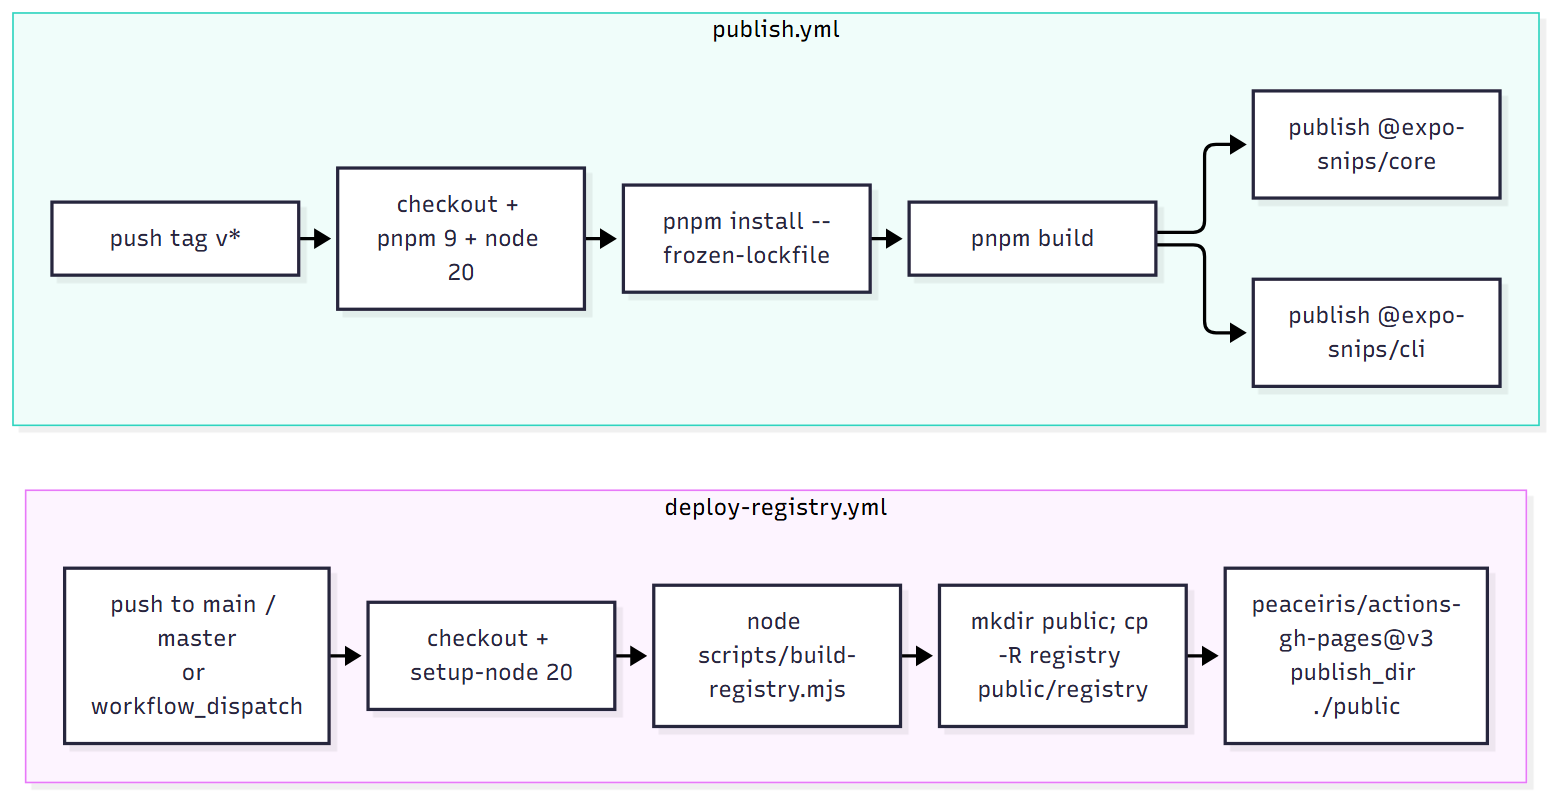
\includegraphics[width=\textwidth]{diagrams/cicd-deployment.png}
\caption{Continuous delivery pipelines present in the repository}
\label{fig:cicd-deployment}
\end{figure}

\section{Workflow inventory}

\begin{longtable}{p{3.2cm}p{3.4cm}p{3.4cm}p{4.2cm}}
\caption{GitHub Actions workflows}\\
\toprule
\textbf{File} & \textbf{Trigger} & \textbf{Runner} & \textbf{Purpose} \\
\midrule

\texttt{publish.yml} & push to tags \texttt{v*} & ubuntu-latest, Node 20,
pnpm 9 & Build all packages and publish \texttt{@expo-snips/core} and
\texttt{@expo-snips/cli} to npm. \\
\texttt{deploy-registry.yml} & push to \texttt{main}/\texttt{master},
\texttt{workflow\_dispatch} & ubuntu-latest, Node 20 & Build the registry and
deploy it to GitHub Pages. \\
\bottomrule
\end{longtable}

\section{Pipeline detail: \texttt{publish.yml}}

\begin{enumerate}
  \item \texttt{actions/checkout@v4}
  \item \texttt{pnpm/action-setup@v4} (version 9)
  \item \texttt{actions/setup-node@v4} (Node 20, \texttt{registry-url:
        https://registry.npmjs.org})
  \item \texttt{pnpm install --frozen-lockfile} --- reproducible install from the
        committed lockfile.
  \item \texttt{pnpm build} --- recursive build; this runs
        \texttt{prepare-registry.mjs} for both clients before compilation.
  \item Publish \texttt{core}, then publish \texttt{cli}, each authenticated with
        \texttt{NPM\_TOKEN}.
\end{enumerate}

Notes: publishing uses \texttt{--no-git-checks} (permitting a publish from a
detached HEAD, which is normal on a tag build) and \texttt{--access public}
(reinforcing the package's own \texttt{publishConfig}). There is no headless
\texttt{npm whoami} check, no provenance/attestation step, and no dry-run gate.

\section{Pipeline detail: \texttt{deploy-registry.yml}}

\begin{enumerate}
  \item \texttt{actions/checkout@v4}
  \item \texttt{actions/setup-node@v4} (Node 20; no dependency install step
        because the script uses only Node built-ins)
  \item \texttt{node scripts/build-registry.mjs} --- rebuilds
        \texttt{registry/}
  \item \texttt{mkdir public} and \texttt{cp -R registry public/registry}
  \item \texttt{peaceiris/actions-gh-pages@v3} publishes \texttt{./public} to
        \texttt{gh-pages} using \texttt{GITHUB\_TOKEN}, under
        \texttt{contents: write} permission.
\end{enumerate}

\section{What the pipelines do not do}

\begin{longtable}{p{4.6cm}p{2.2cm}p{7.4cm}}
\caption{Missing pipeline capabilities}\\
\toprule
\textbf{Capability} & \textbf{Present?} & \textbf{Comment} \\
\midrule

Linting & No & No linter is configured anywhere in the repo. \\
Automated tests & No & No tests exist; no test step is present. \\
Recipe validation in CI & No & \texttt{validate.mjs} exists but is not invoked by
either workflow. \\
Build on pull requests & No & Neither workflow runs on \texttt{pull\_request}. \\
Type checking & Indirect & \texttt{pnpm build} runs \texttt{tsc}, so type errors
fail the delivery build --- but only after merge or on a tag, not on a PR. \\
Dependency audit & No & No \texttt{pnpm audit}, Dependabot or CodeQL. \\
Extension packaging/publish & No & The VSIX is built and committed by hand. \\
Caching & No & No \texttt{actions/cache} or pnpm store cache configured. \\
Provenance / attestation & No & Plain \texttt{npm publish}. \\
Version bumping & No & Version numbers are edited manually in
\texttt{package.json}. \\
\bottomrule
\end{longtable}

\section{Consequences}

\begin{itemize}
  \item \textbf{The pipeline cannot prevent a broken main.} Because no workflow
        runs on pull requests, a change that fails to build or violates the
        recipe schema is only discovered when someone builds locally --- or when
        a tag is pushed and publishing fails.
  \item \textbf{The registry is rebuilt on every push to the default branch.}
        This is good for freshness but means an unreviewed change to a template
        reaches the published registry immediately after merge.
  \item \textbf{The extension lags the rest of the product.} The CLI and registry
        are automated while the extension, the most user-facing artefact, is
        manual.
  \item \textbf{No concurrency control on \texttt{deploy-registry.yml}.} Two rapid
        pushes could race to push the \texttt{gh-pages} branch; there is no
        \texttt{concurrency} group.
\end{itemize}

\section{Recommended pipeline}

\textbf{Status:} RECOMMENDED. A minimal, high-value CI workflow on
\texttt{pull\_request} and \texttt{push} to the default branch would:

\begin{enumerate}
  \item check out, install with \texttt{--frozen-lockfile};
  \item run \texttt{node scripts/validate.mjs} (recipe integrity);
  \item run \texttt{pnpm build} (type-check and compile all packages);
  \item run tests once they exist (see Chapter~\ref{ch:testing});
  \item add a linter and formatter check;
  \item enable dependency update automation.
\end{enumerate}

Then add a \texttt{concurrency} group to the registry deployment workflow and a
tag-triggered job that packages the extension.

\section{CI/CD summary}

\begin{table}[H]
\centering
\caption{CI/CD posture}
\begin{tabular}{p{4cm}p{10.2cm}}
\toprule
\textbf{Dimension} & \textbf{Assessment} \\
\midrule
Continuous integration & NOT IMPLEMENTED (no PR validation). \\
Continuous delivery --- npm & IMPLEMENTED (tag-triggered). \\
Continuous delivery --- registry & IMPLEMENTED (push-triggered). \\
Continuous delivery --- extension & NOT IMPLEMENTED (manual). \\
Quality gates in CI & None beyond compilation. \\
\bottomrule
\end{tabular}
\end{table}

\chapter{Integrations}
\label{ch:integrations}

\section{Integration map}

Expo Snips integrates with external systems in three directions: build-time
tooling, distribution channels, and the developer projects it generates code
into. There is no server-side integration surface (no webhooks, no message
queues, no third-party APIs called at runtime other than an optional registry
fetch).

\begin{longtable}{p{3.1cm}p{2.2cm}p{3.2cm}p{5.6cm}}
\caption{External integrations}\\
\toprule
\textbf{Integration} & \textbf{Direction} & \textbf{Status} & \textbf{Notes} \\
\midrule

npm registry & Outbound (install, publish) & IMPLEMENTED & Dependency install of
generated screens; publishing of the two public packages. \\
GitHub Pages & Outbound (deploy) & IMPLEMENTED & Static hosting of the recipe
registry. \\
VS Code Extension API & Bidirectional (host) & IMPLEMENTED & Commands, completion
provider, status bar, settings, terminals. \\
Remote recipe registry & Inbound (HTTP GET JSON) & IMPLEMENTED (optional,
off-by-default) & Configurable base URL; 10\,s timeout; extension caches 5\,min. \\
GitHub Actions & Platform & IMPLEMENTED & Two delivery workflows. \\
VS Code Marketplace & Outbound (distribution) & NOT IMPLEMENTED & No publish step;
the VSIX is packaged locally. \\
Package managers in target project & Outbound (shell) & IMPLEMENTED & Detects
npm/pnpm/yarn/bun and shells out to install. \\
Analytics / telemetry & --- & NOT APPLICABLE & None present. \\
Authentication providers & --- & NOT APPLICABLE & No accounts, tokens or OAuth. \\
Databases & --- & NOT APPLICABLE & No database. \\
\bottomrule
\end{longtable}

\section{Build-time library integrations}

These are libraries the project itself depends on, not external services.

\begin{longtable}{p{3.2cm}p{3cm}p{6.4cm}}
\caption{Third-party libraries used by the product}\\
\toprule
\textbf{Library} & \textbf{Used by} & \textbf{Role} \\
\midrule

\texttt{handlebars} \^{}4.7.8 & \texttt{core} & Template compilation and
rendering; the generation engine. \\
\texttt{commander} \^{}12 & \texttt{cli} & Command and option parsing. \\
\texttt{prompts} \^{}2.4 & \texttt{cli} & Interactive question prompts. \\
\texttt{chalk} \^{}4.1 & \texttt{cli} & Terminal colour output. \\
\texttt{fs-extra} \^{}11.2 & \texttt{cli}, extension & Directory creation and file
writing. \\
\texttt{esbuild} \^{}0.21 & extension & Bundling the extension to CommonJS. \\
\texttt{@vscode/vsce} \^{}2.24 & extension & Packaging the \texttt{.vsix}. \\
\texttt{typescript} \^{}5.5 & all & Compilation and strict type checking. \\
\bottomrule
\end{longtable}

\textbf{Note on dependency shape:} the CLI and core declare runtime
dependencies; the extension declares its runtime helpers (\texttt{fs-extra},
\texttt{@expo-snips/core}) as \emph{devDependencies} because esbuild bundles them
into the shipped artefact. This is correct for a bundled extension but means the
extension's declared dependency set is not a runtime contract.

\section{Libraries the generated screens depend on}

When a recipe is generated, the tool installs the recipe's declared
dependencies. Across the whole catalog the union is:

\begin{longtable}{p{5.4cm}p{8.8cm}}
\caption{Dependencies declared by recipes}\\
\toprule
\textbf{Package} & \textbf{Used for} \\
\midrule

\texttt{react-hook-form} & Form state management in auth and input screens. \\
\texttt{@hookform/resolvers} & Bridges \texttt{zod} schemas into
\texttt{react-hook-form}. \\
\texttt{zod} & Schema validation for forms. \\
\texttt{lucide-react-native} & Icons (selected when \texttt{icons=lucide}). \\
\texttt{react-native-maps} & The \texttt{map/location} recipe. \\
\texttt{expo-notifications} & The notifications flow. \\
\texttt{class-variance-authority}, \texttt{clsx}, \texttt{tailwind-merge} &
shadcn-style UI primitives and the \texttt{cn} class-merging utility. \\
\bottomrule
\end{longtable}

The generated screens also import modules that are expected to exist in any Expo
project and are therefore not installed by the tool: \texttt{react},
\texttt{react-native}, \texttt{react-native-safe-area-context},
\texttt{expo-router} (the default router) or \texttt{@react-navigation/native}
(when that router is selected), and \texttt{nativewind} (default styling).

\subsection*{Integration gap: \texttt{expo-blur}}

Three templates --- the \texttt{glass} variants of \texttt{app/home},
\texttt{auth/login} and \texttt{onboarding/welcome} --- import
\texttt{BlurView} from \texttt{expo-blur}:

\begin{lstlisting}[language=JavaScript]
import { BlurView } from 'expo-blur';
\end{lstlisting}

However, no recipe declares \texttt{expo-blur} in its \texttt{dependencies}
array, so generating a glass variant does not install the package. A developer
selecting a glass variant would get a module-resolution error until they
installed \texttt{expo-blur} manually.

\textbf{Status:} IMPLEMENTED (templates) / GAP (declared dependency).
\textbf{Recommendation:} declare \texttt{expo-blur} on the three recipes that
offer a glass variant.

\section{The remote registry as an integration}

The registry integration is the only network-facing contract and is worth
treating as a formal API (see Chapter~\ref{ch:api-documentation}). Its
properties:

\begin{itemize}
  \item \textbf{Protocol:} plain HTTPS (or HTTP) GET returning JSON.
  \item \textbf{Endpoints:} \texttt{\{base\}/index.json} and
        \texttt{\{base\}/recipes/\{id\}.json}, where the id contains a slash and
        is therefore URL-encoded by the client.
  \item \textbf{Authentication:} none.
  \item \textbf{Configuration:} CLI \texttt{--registry} or
        \texttt{EXPO\_SNIPS\_REGISTRY}; extension \texttt{expo-snips.registryUrl}.
  \item \textbf{Resilience:} 10-second timeouts; the extension caches for 5
        minutes and falls back to its embedded catalog on failure; the CLI falls
        back to its embedded catalog when no base is configured.
  \item \textbf{Failure mode:} a non-2xx response or malformed shape causes an
        error on the CLI and a silent fallback on the extension.
\end{itemize}

\section{Integration risks}

\begin{itemize}
  \item A user-configured registry becomes a trusted code channel with no
        signature or hash verification (see Chapter~\ref{ch:security}).
  \item The hard-coded default host \texttt{registry.expo-snips.dev} is not
        represented in the repository by any hosting configuration, so its
        liveness is \textbf{UNKNOWN}.
  \item The extension's ``fallback to embedded catalog'' behaviour is helpful but
        means a misconfigured registry silently produces the built-in catalog
        rather than an error, which can mask configuration mistakes.
\end{itemize}

\section{Summary}

\textbf{Status:} IMPLEMENTED (build tooling, npm, GitHub Pages, VS Code API,
optional registry) / NOT IMPLEMENTED (Marketplace publishing) / NOT APPLICABLE
(analytics, auth providers, databases).

\chapter{Configuration}
\label{ch:configuration}

\section{Configuration surfaces}

Expo Snips has no configuration file of its own and no server-side
configuration. Configuration exists at four points:

\begin{enumerate}
  \item \textbf{CLI flags and environment variables} (command line / process
        environment).
  \item \textbf{VS Code settings} (editor settings, per user or workspace).
  \item \textbf{Recipe definitions} (JSON data that configures generation
        behaviour per screen).
  \item \textbf{Per-project state} (the \texttt{.expo-snips.json} manifest and
        the detected stack of the user's project).
\end{enumerate}

There is no \texttt{.env} file in the repository and none is read by the code.

\section{Environment variables}

\begin{longtable}{p{4.4cm}p{2.2cm}p{7.6cm}}
\caption{Environment variables}\\
\toprule
\textbf{Variable} & \textbf{Default} & \textbf{Effect} \\
\midrule

\texttt{EXPO\_SNIPS\_REGISTRY} & empty (embedded catalog) & Overrides the
registry base URL used by the CLI. An empty value selects the embedded catalog. \\
\texttt{PORT} & \texttt{3000} & Port for the development registry server
(\texttt{scripts/serve.mjs}). \\
\texttt{NPM\_TOKEN} & --- & CI only. Authenticates npm publishing in
\texttt{publish.yml}. Never read by application code. \\
\texttt{GITHUB\_TOKEN} & --- & CI only. Used by the Pages deploy action. Never
read by application code. \\
\bottomrule
\end{longtable}

\textbf{Precedence (CLI):} an explicit \texttt{--registry} flag takes precedence
over \texttt{EXPO\_SNIPS\_REGISTRY}; when neither is set, the built-in default
registry constant applies. An empty string in either place means ``use the
catalog bundled with the package''.

\section{CLI options}

Global and per-command options are defined with \texttt{commander}. The
generation-relevant options are:

\begin{longtable}{p{3.4cm}p{3.4cm}p{6.8cm}}
\caption{CLI generation options}\\
\toprule
\textbf{Option} & \textbf{Values} & \textbf{Effect} \\
\midrule

\texttt{--styling} & \texttt{nativewind}, \texttt{stylesheet},
\texttt{tamagui} & Selects the styling template branch; validated against the
recipe's \texttt{supported.styling}. \\
\texttt{--router} & \texttt{expo-router}, \texttt{react-navigation} & Selects the
navigation template branch; validated against
\texttt{supported.router}. \\
\texttt{--ui} & \texttt{native}, \texttt{shadcn}, \texttt{custom} & Selects the UI
primitive branch; \texttt{shadcn} additionally forces
\texttt{styling=nativewind} and \texttt{icons=lucide} and pulls in primitive
recipes. \\
\texttt{--icons} & \texttt{lucide}, \texttt{vector-icons}, \texttt{none} &
Selects the icon template branch. \\
\texttt{--variant} & \textit{recipe-defined} & Selects a named template variant.
Not validated against the recipe. \\
\texttt{--typescript} / \texttt{--javascript} & flag & Forces the language branch
(overrides detection). \\
\texttt{--no-install} & flag & Skips dependency installation. \\
\texttt{--registry <url>} & URL & Overrides the registry base URL. \\
\bottomrule
\end{longtable}

When an option is omitted, the value is inferred from the project (see below),
then falls back to a default, then to an interactive prompt if the terminal is
interactive.

\section{VS Code settings}

The extension contributes a configuration section titled ``Expo Snips'' with
these properties:

\begin{longtable}{p{4.2cm}p{1.8cm}p{2.4cm}p{5.8cm}}
\caption{VS Code settings}\\
\toprule
\textbf{Setting} & \textbf{Type} & \textbf{Default} & \textbf{Effect} \\
\midrule

\texttt{expo-snips.registryUrl} & string & \textit{empty} & Remote registry base.
Empty uses the embedded catalog. \\
\texttt{expo-snips.defaultStyling} & enum & \texttt{nativewind} & Fallback styling
when detection fails. Values: \texttt{nativewind}, \texttt{stylesheet},
\texttt{tamagui}. \\
\texttt{expo-snips.defaultRouter} & enum & \texttt{expo-router} & Fallback router.
Values: \texttt{expo-router}, \texttt{react-navigation}. \\
\texttt{expo-snips.defaultUi} & enum & \texttt{native} & Fallback UI primitives.
Values: \texttt{native}, \texttt{shadcn}, \texttt{custom}. \\
\texttt{expo-snips.defaultIcons} & enum & \texttt{lucide} & Fallback icon library.
Values: \texttt{lucide}, \texttt{vector-icons}, \texttt{none}. \\
\texttt{expo-snips.installDependencies} & boolean & \texttt{true} & Install
recipe dependencies in a terminal after generation. \\
\bottomrule
\end{longtable}

\textbf{Configuration mismatch to note:} the settings enums advertise
\texttt{tamagui}, \texttt{vector-icons} and \texttt{custom}, but no recipe in the
catalog currently implements them (every recipe's \texttt{supported} array
excludes them). Selecting such a fallback would have no recipe to match. The
extension README acknowledges this. This is a documentation/configuration
inconsistency rather than a runtime defect, but it can mislead users.

\section{Project detection (configuration by inference)}

The tool configures itself from the target project rather than requiring input.
Detection reads:

\begin{longtable}{p{4.6cm}p{9.6cm}}
\caption{Detection probes}\\
\toprule
\textbf{Setting} & \textbf{Probe} \\
\midrule

Router & \texttt{expo-router} present in dependencies selects
\texttt{expo-router}; otherwise \texttt{@react-navigation/native} selects
\texttt{react-navigation}. \\
Styling & \texttt{nativewind} in dependencies selects \texttt{nativewind};
otherwise \texttt{stylesheet}. \\
UI primitives & \texttt{@shadcn/ui} or \texttt{react-native-reusables} selects
\texttt{shadcn}; otherwise \texttt{native}. \\
Icons & \texttt{lucide-react-native} selects \texttt{lucide}; otherwise
\texttt{none}. \\
TypeScript & Presence of \texttt{tsconfig.json}. \\
\bottomrule
\end{longtable}

\textbf{Status:} IMPLEMENTED. Detected values are used as defaults; explicit
flags (CLI) or settings fallbacks (extension) take precedence.

\section{Recipe-level configuration}

Recipes are the richest configuration surface. A recipe declares:

\begin{itemize}
  \item its identity and version (\texttt{id}, \texttt{name}, \texttt{description},
        \texttt{version});
  \item the options it \emph{supports} (\texttt{supported.styling/router/ui/icons})
        --- the tool will only generate combinations a recipe declares;
  \item its \texttt{dependencies} and \texttt{devDependencies};
  \item its \texttt{files}, each with a target \texttt{path}, a
        \texttt{templateFile}, an optional \texttt{when} condition, and optional
        \texttt{variants} and \texttt{perStyling} template overrides;
  \item optional \texttt{variants} (named style alternatives),
        \texttt{tags} (search keywords) and \texttt{primitives} (UI primitive
        recipes required when \texttt{ui=shadcn}).
\end{itemize}

The authoritative machine-readable definition is
\texttt{packages/registry/schema.json} (JSON Schema Draft-07), reproduced in
Chapter~\ref{ch:registry-and-recipes}.

\section{Project state: the manifest}

\begin{lstlisting}[language=JavaScript]
// .expo-snips.json  (written into the user's project root)
interface Manifest {
  version: number;
  screens: Array<{
    recipeId: string;
    recipeVersion: string;
    variant?: string;
    options: GenerationOptions;
    files: string[];
    installedAt: string;
  }>;
}
\end{lstlisting}

The manifest is created by the tool, written with two-space indentation, and
tolerates absent or unreadable content by treating the project as having no
tracked screens. The upsert key for a screen is the recipe id \emph{plus} the
variant, so the same recipe can be tracked once per variant.

\section{Build and development configuration}

\begin{longtable}{p{4.4cm}p{9.8cm}}
\caption{Build-related configuration}\\
\toprule
\textbf{File} & \textbf{Purpose} \\
\midrule

\texttt{pnpm-workspace.yaml} & Declares \texttt{packages/*} and an
\texttt{allowBuilds} policy that enables build scripts for \texttt{esbuild} and
\texttt{@vscode/vsce-sign} and disables them for \texttt{keytar}. \\
\texttt{tsconfig.base.json} & Shared TypeScript compiler options extended by each
package. \\
Per-package \texttt{tsconfig.json} & Package-specific compilation settings. \\
\texttt{esbuild.mjs} & Bundle configuration for the extension (CJS, Node 18
target, \texttt{vscode} external, sourcemap on). \\
\texttt{.vscodeignore} & Excludes sources and dev material from the packaged
VSIX. \\
\texttt{.gitignore} & Excludes build output and generated files from version
control. \\
\bottomrule
\end{longtable}

There is no \texttt{eslint}, \texttt{prettier} or \texttt{editorconfig}
configuration in the repository.

\section{Configuration summary}

\begin{table}[H]
\centering
\caption{Configuration posture}
\begin{tabular}{p{4.4cm}p{9.8cm}}
\toprule
\textbf{Surface} & \textbf{Assessment} \\
\midrule
CLI flags / env & IMPLEMENTED; documented in Chapter~\ref{ch:cli-reference}. \\
Editor settings & IMPLEMENTED; three values advertise unimplemented options. \\
Recipe data & IMPLEMENTED; schema-governed. \\
Detection & IMPLEMENTED; four probes plus a TypeScript probe. \\
Config files & NOT APPLICABLE (none exists). \\
Secrets & None in the application; CI secrets only. \\
\bottomrule
\end{tabular}
\end{table}


% ---------------------------------------------------------------------
%  Part VII: Discoverability
% ---------------------------------------------------------------------
\chapter{SEO --- Search Engine Optimisation}
\label{ch:seo}

\section{Applicability}

\textbf{Classic web SEO:} NOT APPLICABLE. The project publishes no website, no
landing page, no HTML documentation site and no marketing URL. There is no
\texttt{index.html}, no \texttt{robots.txt}, no \texttt{sitemap.xml} and no
rendered content for a search engine to index. The only HTTP surface the project
owns is the recipe registry, which serves machine-readable JSON.

\textbf{Discoverability SEO:} APPLICABLE. The product is discovered through three
\textbf{listing} channels that function as its search surface, and these are
where optimisation is meaningful:

\begin{enumerate}
  \item the npm registry (for \texttt{@expo-snips/core} and
        \texttt{@expo-snips/cli});
  \item the VS Code Marketplace listing (for the \texttt{expo-snippets}
        extension);
  \item GitHub repository search and general web search of repository content.
\end{enumerate}

This chapter therefore analyses the metadata that governs discovery in those
channels.

\section{In-repository SEO signals}

\begin{longtable}{p{3.6cm}p{3.2cm}p{7.4cm}}
\caption{SEO-relevant metadata found in the repository}\\
\toprule
\textbf{Artefact} & \textbf{Signal} & \textbf{Content} \\
\midrule

Extension \texttt{package.json} & \texttt{displayName} & ``Expo Snippets''. \\
Extension \texttt{package.json} & \texttt{description} & ``Generate complete React
Native screens with a single abbreviation.'' \\
Extension \texttt{package.json} & \texttt{keywords} & Over 40 keywords covering
\texttt{react-native}, \texttt{expo}, \texttt{screen}, \texttt{template},
\texttt{codegen}, \texttt{expo-router}, \texttt{nativewind}, \texttt{shadcn},
\texttt{vscode}, \texttt{expo-snips} and more. \\
Extension \texttt{package.json} & \texttt{categories} & \texttt{Snippets},
\texttt{Other}. \\
Extension \texttt{package.json} & \texttt{repository.url} & Links to
\texttt{github.com/unkown812/expo-snips}. \\
Extension \texttt{package.json} & \texttt{icon} & \texttt{assets/logo.png}. \\
Extension README & Rich Markdown & Headings, tables, feature lists, quick-start
instructions, badges. \\
CLI \texttt{package.json} & \texttt{description} & ``Beautiful React Native
screens, one command away.'' \\
Core \texttt{package.json} & \texttt{description} & ``Shared types and generation
engine for Expo Snips screens.'' \\
Repository & Topic titles & Recipe names and descriptions provide natural-language
keywords (\texttt{auth/login}, \texttt{onboarding/welcome}, \dots). \\
\bottomrule
\end{longtable}

\section{Strengths}

\begin{itemize}
  \item The extension keyword list is unusually broad and covers the phrases a
        developer would actually search (\texttt{react-native screen generator},
        \texttt{expo template}, \texttt{codegen}, framework names). Keyword
        coverage is the strongest discovery asset the project has.
  \item The extension README is substantial and structured, which is favourable
        both to the Marketplace listing and to GitHub search.
  \item The \texttt{repository} field and README links create a coherent
        cross-channel trail from listing to source.
\end{itemize}

\textbf{Status:} IMPLEMENTED.

\section{Gaps}

\begin{longtable}{p{1.5cm}p{4.6cm}p{3.4cm}p{4.7cm}}
\caption{SEO findings}\\
\toprule
\textbf{ID} & \textbf{Finding} & \textbf{Evidence} & \textbf{Recommendation} \\
\midrule

SEO-01 & No website or landing page exists, so every search result resolves to a
repository or a listing rather than a product page. & Absence of any HTML in the
repo. & If a product identity is intended, publish a small static site with
descriptive copy. \\
SEO-02 & No root README. The top-level repository view shows no descriptive text,
which weakens GitHub search relevance and first impressions. & Absence of
\texttt{README.md} at the repository root. & Add a root README that describes the
monorepo and links the packages. \\
SEO-03 & npm packages carry only the \texttt{description} field as prose; there is
no \texttt{README} referenced from the npm listing and no keywords field on the
npm packages. & \texttt{packages/*/package.json}. & Add \texttt{keywords} and
ensure a README is published with each npm package. \\
SEO-04 & Listing metadata is inconsistent: the extension's repository/author
(\texttt{unkown812}) differs from the owner host implied by some README links
(\texttt{github.com/expo-snips/expo-snips}). & \texttt{package.json} vs README
links. & Standardise the canonical repository URL everywhere. \\
SEO-05 & The registry serves JSON only; nothing about the recipes is
human-browsable or indexable. & \texttt{scripts/serve.mjs}, \texttt{registry/}. &
Optionally publish a human-readable catalog page generated from the index. \\
\bottomrule
\end{longtable}

\section{Summary}

\begin{table}[H]
\centering
\caption{SEO posture}
\begin{tabular}{p{4.6cm}p{9.6cm}}
\toprule
\textbf{Dimension} & \textbf{Assessment} \\
\midrule
Website SEO & NOT APPLICABLE (no website). \\
Listing keyword coverage & IMPLEMENTED and strong (extension keywords). \\
npm discoverability & PARTIAL (descriptions only). \\
Repository discoverability & PARTIAL (no root README). \\
Cross-channel consistency & Needs work (repository URL mismatch). \\
\bottomrule
\end{tabular}
\end{table}

\textbf{Status:} NOT APPLICABLE (web SEO) / PARTIAL (listing SEO) / RECOMMENDED
(root README, canonical URLs).

\chapter{AEO --- Answer Engine Optimisation}
\label{ch:aeo}

\section{Applicability}

Answer Engine Optimisation concerns how readily a product's content is selected
and quoted by answer engines --- AI assistants, conversational search and
featured-snippet surfaces. As with SEO (Chapter~\ref{ch:seo}), there is no
project-owned website, so the question reduces to: \emph{how well does the
repository and its listings feed answer engines?}

\section{Content available to answer engines}

Answer engines draw on: the README files, the package metadata, the recipe
descriptions, the extension CHANGELOG, and any prose in the repository. All of
these are plain text or Markdown, which is exactly the format answer engines can
consume and quote.

\begin{longtable}{p{4.4cm}p{3.2cm}p{6.6cm}}
\caption{Answer-engine-relevant content}\\
\toprule
\textbf{Source} & \textbf{Format} & \textbf{Value for answer engines} \\
\midrule

Extension README & Markdown & Explains what the tool does, the problem it solves,
and how to use it, in natural language. \\
\texttt{ProjectDescription.md} & Markdown & A product description with framing that
answers ``what is this?''. \\
Recipe \texttt{description} fields & Plain text & One-line answers to ``is there a
screen for X?''. \\
Extension CHANGELOG & Markdown & Dated, factual statements suitable for quoting. \\
Package descriptions & Plain text & Short capability statements. \\
\bottomrule
\end{longtable}

\section{Answer-readiness of the content}

\begin{longtable}{p{1.5cm}p{4.6cm}p{3.4cm}p{4.7cm}}
\caption{AEO findings}\\
\toprule
\textbf{ID} & \textbf{Finding} & \textbf{Evidence} & \textbf{Recommendation} \\
\midrule

AEO-01 & The repository contains clear ``what it is / what problem'' prose in the
extension README, which is well suited to being quoted verbatim. & Extension
README sections ``What is Expo Snips?'' and ``The Problem''. & IMPLEMENTED; keep
this structure. \\
AEO-02 & FAQ-shaped content is absent. Answer engines favour explicit question-and-answer
pairings that can be lifted directly. & No FAQ section anywhere. & RECOMMENDED:
add a short FAQ (``Does it work offline?'', ``Which Expo SDK?'', ``Is it free?''). \\
AEO-03 & \texttt{documents/ProjectDescription.md} contains \emph{outdated}
statements: it references a recipe count and variant support that the code no
longer matches. & \texttt{documents/ProjectDescription.md}. & Update it, because
an answer engine may quote the stale figure. See
Chapter~\ref{ch:known-issues}. \\
AEO-04 & Authoritative one-sentence definitions are duplicated in several places
(README, package descriptions) with slightly different wording, which can produce
inconsistent answers. & \texttt{vscode-extension/package.json} description vs
README headline. & Standardise a single canonical one-liner. \\
AEO-05 & No structured data (schema.org \texttt{SoftwareApplication} or
\texttt{SoftwareSourceCode}) is published, because there is no site to host it. &
Absence of any HTML. & NOT APPLICABLE unless a site is created; then add JSON-LD. \\
AEO-06 & The README uses license and version badges that are useful, unambiguous
facts for an answer engine to extract. & Badge block in the extension README. &
IMPLEMENTED. \\
\bottomrule
\end{longtable}

\section{Factual accuracy as an AEO risk}

The single most important AEO property is accuracy; an answer engine that quotes
a wrong fact damages trust more than one that quotes nothing. Two facts about
this repository are stated inconsistently across sources:

\begin{itemize}
  \item \textbf{Recipe count:} \texttt{ProjectDescription.md} understates the
        catalog relative to the code, where the count is 24.
  \item \textbf{Variant support:} \texttt{ProjectDescription.md} implies variants
        are unsupported, while three recipes (\texttt{app/home},
        \texttt{auth/login}, \texttt{onboarding/welcome}) implement a
        \texttt{glass} variant.
\end{itemize}

\textbf{Status:} INFERRED from comparison of the document with the code.
\textbf{Recommendation:} correct the description document (RECOMMENDED).

\section{Summary}

\begin{table}[H]
\centering
\caption{AEO posture}
\begin{tabular}{p{4.6cm}p{9.6cm}}
\toprule
\textbf{Dimension} & \textbf{Assessment} \\
\midrule
Quotable capability prose & IMPLEMENTED (extension README). \\
FAQ content & ABSENT (recommended). \\
Structured data & NOT APPLICABLE (no site). \\
Factual consistency & GAP (outdated description document). \\
\bottomrule
\end{tabular}
\end{table}

\textbf{Status:} PARTIAL / RECOMMENDED.

\chapter{GEO --- Generative Engine Optimisation}
\label{ch:geo}

\section{Applicability and scope}

Generative Engine Optimisation concerns whether a product is represented and
cited accurately by generative systems: large language models and the assistants
built on them, including code-generating assistants. For a developer tool, GEO
matters because a common way a developer learns about a library is to ask an
assistant ``how do I scaffold an Expo login screen?''.

There is no project-owned website to optimise, so classic GEO tactics
(rich pages, citations, entity markup) are \textbf{NOT APPLICABLE}. What is
applicable is the \emph{corpus footprint}: whether the project's own material is
present, self-consistent and machine-consumable where generative systems look.

\section{Corpus footprint}

\begin{longtable}{p{4.4cm}p{2.8cm}p{7cm}}
\caption{Sources a generative system could learn from}\\
\toprule
\textbf{Source} & \textbf{Availability} & \textbf{Content} \\
\midrule

Public GitHub repository & Public (master branch) & Source, recipes, templates,
workflows, READMEs. \\
npm packages & Public & \texttt{@expo-snips/core}, \texttt{@expo-snips/cli}
metadata and (if a README is published) documentation. \\
VS Code Marketplace listing & Public (when listed) & Extension metadata, README,
keywords. \\
Recipe registry JSON & Public & Structured catalog with descriptions and tags. \\
Answering-assistant context & Not controlled & Unknown whether any model has been
trained on or cites this project. \\
\bottomrule
\end{longtable}

\section{Generative-readiness properties}

\begin{itemize}
  \item \textbf{Structured, self-describing data:} the recipe catalog is JSON
        Schema-conformant, with \texttt{id}, \texttt{name}, \texttt{description}
        and \texttt{tags} per recipe. This is precisely the shape a generative
        system can reason over, and it is a genuine strength.
  \item \textbf{Machine-readable API documentation:} the \texttt{@expo-snips/core}
        package ships TypeScript declarations, and the generated
        \texttt{registry-data.ts} is typed, giving models accurate signatures.
  \item \textbf{Versioned, dated history:} the extension CHANGELOG is dated and
        factual.
  \item \textbf{No telemetry or private corpus:} nothing about the tool's usage is
        captured, so there is no private signal to leak or misrepresent.
\end{itemize}

\textbf{Status:} IMPLEMENTED.

\section{Representation risks}

\begin{longtable}{p{1.5cm}p{4.6cm}p{3.4cm}p{4.7cm}}
\caption{GEO findings}\\
\toprule
\textbf{ID} & \textbf{Finding} & \textbf{Evidence} & \textbf{Recommendation} \\
\midrule

GEO-01 & Inconsistent identity across sources: the extension publishes under
publisher \texttt{ukown812} and repository \texttt{github.com/unkown812/expo-snips},
while some README links point at \texttt{github.com/expo-snips/expo-snips}. A
generative system may conflate these into a wrong citation. & Extension
\texttt{package.json} vs README links. & Canonicalise one repository URL and apply
it everywhere. \\
GEO-02 & Name collision risk: the extension is published as \texttt{expo-snippets},
the CLI as \texttt{@expo-snips/cli}, and the product as ``Expo Snips''. Models may
treat these as three products. & \texttt{package.json} names. & Keep the
``Expo Snips'' brand string adjacent to each package name in its description. \\
GEO-03 & Stale prose in \texttt{ProjectDescription.md} can propagate an
incorrect fact (recipe count, variant support) into a generated answer. &
\texttt{documents/ProjectDescription.md}. & Correct the document; keep a single
source of truth for counts. \\
GEO-04 & No license clarity for the extension beyond ``Private License'', which a
generative system cannot interpret as a known SPDX license. & Extension
\texttt{package.json} \texttt{license} field. & Use an explicit, recognisable
license expression if the intent allows. \\
GEO-05 & No canonical, quotable ``what is this'' one-liner shared across sources. &
Three differing descriptions. & Publish one canonical sentence and reuse it. \\
\bottomrule
\end{longtable}

\section{Why GEO matters for this product specifically}

The product's value proposition --- ``generate a complete, correct screen for a
given stack'' --- is exactly the kind of question developers pose to coding
assistants. If a model has never seen the project or cites it inconsistently, the
assistant will instead suggest generic manual boilerplate, which is the
alternative the tool exists to replace. GEO is therefore economically meaningful
even without a website: the goal is that a generative system, asked for an Expo
screen, can name the tool and be correct about what it does.

\section{Summary}

\begin{table}[H]
\centering
\caption{GEO posture}
\begin{tabular}{p{4.6cm}p{9.6cm}}
\toprule
\textbf{Dimension} & \textbf{Assessment} \\
\midrule
Website/entity optimisation & NOT APPLICABLE (no site). \\
Structured corpus & IMPLEMENTED (schema-valid JSON, typed declarations). \\
Identity consistency & GAP (publisher/repo/brand mismatch). \\
Factual consistency & GAP (stale description document). \\
Model citations & UNKNOWN (not observable from the repository). \\
\bottomrule
\end{tabular}
\end{table}

\textbf{Status:} PARTIAL / RECOMMENDED (canonical identity, accurate descriptions).


% ---------------------------------------------------------------------
%  Part VIII: Maintenance and evolution
% ---------------------------------------------------------------------
\chapter{Known Issues}
\label{ch:known-issues}

\section{Purpose and method}

This chapter records defects, inconsistencies and behavioural surprises that are
\emph{present in the code as analysed}. It does not duplicate security findings,
which are catalogued in Chapter~\ref{ch:security}, nor the maintenance backlog in
Chapter~\ref{ch:technical-debt}. Each issue is given an identifier, a category, a
severity and an evidence pointer. Severity reflects impact on a user of the
product: \textbf{High} means wrong or broken generated output in a plausible
workflow, \textbf{Medium} means confusion or a manual workaround, \textbf{Low}
means cosmetic or documentation-only.

Some issues are documented by the authors themselves (the extension README's
``Known Limitations'' and the CHANGELOG), and these are marked accordingly.

\section{Issue register}

\begin{longtable}{p{1.2cm}p{3.3cm}p{1.6cm}p{1.1cm}p{6.4cm}}
\caption{Known issues}\\
\toprule
\textbf{ID} & \textbf{Category} & \textbf{Severity} & \textbf{Status} &
\textbf{Description and evidence} \\
\midrule

KI-01 & Generated styling & High & Open & shadcn-generated screens use design tokens
such as \texttt{bg-background}, \texttt{text-foreground},
\texttt{border-border} and \texttt{ring-ring}, but the repository ships no
Tailwind/NativeWind theme configuration defining those tokens. A generated shadcn
screen can therefore render unstyled until the user adds the token definitions.
Evidence: shadcn templates under \texttt{packages/registry/templates}; no
\texttt{tailwind.config.*} in the repository. \\
KI-02 & Missing dependency & High & Open & The \texttt{glass} variants of
\texttt{app/home}, \texttt{auth/login} and \texttt{onboarding/welcome} import
\texttt{expo-blur}, which no recipe declares in \texttt{dependencies}; the package
is not installed. Evidence: \texttt{*.glass.hbs} template imports; recipe JSON
dependency arrays. \\
KI-03 & Interactive generation & High & Open (documented) & Auth hooks generated by
\texttt{auth/login} and \texttt{auth/register} are placeholders: they wait a fixed
delay and then always report success. The shadcn login form only
\texttt{console.log}s the submitted data and does not call the hook at all.
Shipping without replacement yields a non-functional login. Evidence:
\texttt{hooks.use-login.hbs}, \texttt{hooks.use-register.hbs},
\texttt{components.login-form.shadcn.hbs}. \\
KI-04 & Advertised-but-unimplemented options & Medium & Open (documented) &
\texttt{tamagui}, \texttt{vector-icons} and \texttt{custom} are offered in the
extension settings and exist in the schema, but no recipe implements them.
Selecting one finds no matching recipe. Evidence: extension
\texttt{package.json} enums vs recipe \texttt{supported} arrays. \\
KI-05 & CLI version reporting & Medium & Open & The CLI's \texttt{--version} output
is a hard-coded literal rather than the package version, so it will drift from
\texttt{package.json} on release. Evidence:
\texttt{packages/cli/src/index.ts}. \\
KI-06 & Silent overwrite & Medium & Open & \texttt{add} overwrites any existing file
at a recipe path without confirmation or backup; only primitive files are
skip-aware. Evidence: \texttt{cli/src/utils/writeFiles.ts}. (Also logged as
SEC-16.) \\
KI-07 & Variant validation & Medium & Open & An unknown \texttt{--variant} value is
silently ignored and the default template is produced, with no warning. Evidence:
\texttt{core/src/generate.ts} \texttt{resolveTemplateString}. \\
KI-08 & Silent fallback & Medium & Open & When a configured remote registry is
unreachable, the extension silently uses its built-in catalog; the user cannot
tell that their configured registry was ignored. Evidence: extension
\texttt{registry.ts} fallback path. \\
KI-09 & Stale product document & Medium & Open & \texttt{documents/ProjectDescription.md}
understates the catalog and implies variants are unsupported, contradicting the
code (24 recipes; variants present). Evidence: document vs
\texttt{packages/registry/data/**} and \texttt{registry/index.json}. \\
KI-10 & Partial-failure consistency & Low & Open & If dependency installation
fails, generated files have already been written and the manifest may not be
updated, leaving files and manifest disagreeing. Evidence: ordering in
\texttt{cli/src/commands/add.ts}. (Also logged as SEC-17.) \\
KI-11 & Credential logging & Low & Open & Generated auth code logs submitted
credentials to the console. Evidence: auth hook templates. (Also logged as
SEC-12.) \\
KI-12 & Manifest tolerance & Low & Open & A malformed or unreadable
\texttt{.expo-snips.json} is treated as an empty manifest rather than reported, so
corruption is silent. Evidence: \texttt{cli/src/utils/manifest.ts}. \\
KI-13 & Generated artefacts retained in the tree & Low & Open & Two build
outputs are kept in the working tree: the built registry
(\texttt{registry/}, 25 files) and the offline bundle
(\texttt{packages/registry/bundle.json}) are \emph{tracked} by git, while four
packaged extensions (\texttt{expo-snippets-0.1.0..0.1.3.vsix}) sit untracked in
the extension directory (excluded by a \texttt{*.vsix} rule in
\texttt{.gitignore}). Tracking generated files invites drift from source.
Evidence: \texttt{git ls-files}, \texttt{.gitignore}. \\
KI-14 & Registry host unverifiable & Low & Unknown & The CLI's default registry
host \texttt{registry.expo-snips.dev} has no hosting configuration in the
repository, so its existence and ownership cannot be verified here. Evidence:
registry resolution constants; no CNAME or pages config. \\
KI-15 & Generated registry tracked in git & Low & Open & Because
\texttt{registry/} is tracked \emph{and} regenerated on every push to the default
branch, the deployed output and the committed copy can diverge if the deploy
workflow's build differs from a manual build. The single source of truth is
\texttt{packages/registry/data/}. Evidence: \texttt{git ls-files registry};
\texttt{deploy-registry.yml}. \\
\bottomrule
\end{longtable}

\section{Resolved since the initial documentation}

The 1.0 release of this document set (17 October 2026) did not record two
template defects that were discovered the following day while generating every
screen for the repository's screenshot set. Both were fixed in the source
templates on 19 October 2026 and are documented in \texttt{CHANGELOG.md}
(Unreleased section).

\begin{longtable}{p{1.6cm}p{4.6cm}p{4.4cm}p{3.4cm}}
\caption{Resolved template defects (19 October 2026)}\\
\toprule
\textbf{ID} & \textbf{Defect} & \textbf{Evidence} & \textbf{Resolution} \\
\midrule

RS-01 & JSX object literals written as \texttt{\{\{ uri: ... \}\}},
\texttt{initialRegion=\{\{...\}\}} and \texttt{style=\{\{...\}\}} were parsed by
Handlebars as helper calls, so \texttt{chat/conversations},
\texttt{content/article-reader} and \texttt{map/location} crashed at generation
(\emph{Missing helper: ``uri:''}; a parse error in the map template).
\textbf{Status:} IMPLEMENTED (fixed). &
\texttt{templates/chat/conversations/components.conversation-item.hbs},
\texttt{templates/content/article-reader/app.article.[id].hbs},
\texttt{templates/map/location/app.map.index.hbs}. &
Escaped literals (\texttt{\textbackslash\{\{}). All three recipes generate correctly;
\texttt{pnpm validate} reports 0 errors. \\
RS-02 & Component props and calendar helpers were emitted without TypeScript
types, so generated output failed \texttt{tsc --noEmit} in strict projects
(implicit \texttt{any}).
\textbf{Status:} IMPLEMENTED (fixed). &
\texttt{components.conversation-item.hbs}, \texttt{components.event-item.hbs},
\texttt{components.location-sheet.hbs}, \texttt{app.calendar.index.hbs}. &
Typed props/parameters added behind the catalog's existing
\texttt{\{\{#if typescript\}\}} guard. \\
\bottomrule
\end{longtable}

These entries are listed here rather than in the open issue register because
they no longer reproduce against the current tree.

\section{Author-acknowledged limitations}

The extension README's ``Known Limitations'' section explicitly states: no tests;
no CI/CD for the extension (packaged manually); limited icon/styling options
(\texttt{tamagui}, \texttt{vector-icons}, \texttt{custom} unsupported); offline
by default; and VS Code only (the extension and CLI are independently installed).
These align with KI-02 through KI-05 above and with the findings in
Chapter~\ref{ch:testing} and Chapter~\ref{ch:cicd}.

\textbf{Status:} IMPLEMENTED (documented by the authors). This is a positive
practice --- the limitations are stated rather than hidden.

\section{Corrections required to prior documentation}

Two specific corrections are needed to bring the pre-existing
\texttt{ProjectDescription.md} into agreement with the code:

\begin{longtable}{p{5.2cm}p{4.2cm}p{4.6cm}}
\caption{Documentation corrections}\\
\toprule
\textbf{Claim as written} & \textbf{Code reality} & \textbf{Correction} \\
\midrule

An earlier recipe count (stated as 19). & 24 recipes in
\texttt{packages/registry/data}. & Update the count to 24. \\
Variants described as unsupported. & \texttt{app/home}, \texttt{auth/login} and
\texttt{onboarding/welcome} define a \texttt{glass} variant. & Document variant
support and the three recipes that use it. \\
\bottomrule
\end{longtable}

\section{Issue density by area}

\begin{table}[H]
\centering
\caption{Issues by category}
\begin{tabular}{p{5cm}p{4cm}p{5cm}}
\toprule
\textbf{Category} & \textbf{Count} & \textbf{Highest severity} \\
\midrule
Generated output correctness & 3 (KI-01, KI-02, KI-03) & High \\
Configuration / UX & 4 (KI-04, KI-05, KI-07, KI-08) & Medium \\
Data integrity & 3 (KI-06, KI-10, KI-12) & Medium \\
Documentation / hygiene & 5 (KI-09, KI-11, KI-13, KI-14, KI-15) & Medium \\
\bottomrule
\end{tabular}
\end{table}

\section{Summary}

\textbf{Status:} the product is a functioning, coherent tool, but three
high-severity issues affect the \emph{output} it produces: shadcn styling tokens
without theme configuration (KI-01), an undeclared \texttt{expo-blur} import on
glass variants (KI-02), and placeholder authentication code that a developer
might ship unmodified (KI-03). These are the items to address first because they
undermine the product's core promise of ``production-quality screens''.

\chapter{Technical Debt}
\label{ch:technical-debt}

\section{Definition and method}

Technical debt here means maintenance cost accepted in the current codebase:
missing safety nets, duplication, hard-coded values, and structure that will
resist change. Each item has an identifier, an estimate of the interest it
accrues (how much it will slow future work), the evidence, and a recommended
action. Items are ordered by the value of paying them down.

This is distinct from Chapter~\ref{ch:known-issues}, which describes observable
defects. Some findings appear in both where a defect is also a structural
weakness.

\section{Debt register}

\begin{longtable}{p{1.2cm}p{3.6cm}p{1.7cm}p{7.1cm}}
\caption{Technical debt register}\\
\toprule
\textbf{ID} & \textbf{Item} & \textbf{Interest} & \textbf{Evidence and consequence} \\
\midrule

TD-01 & No automated tests anywhere. & High & Absence of any test file. Every
change to the shared core engine or to a template is unverified except by hand;
regressions reach users. The core engine is used by two clients, so a single
mistake is amplified. \\
TD-02 & No linting or formatting configuration. & Medium & No \texttt{eslint},
\texttt{prettier} or \texttt{editorconfig}. Style is upheld by convention only;
diffs carry incidental noise and code quality is inconsistent. \\
TD-03 & No continuous integration on pull requests. & High & Neither workflow runs
on \texttt{pull\_request}. Broken builds and invalid recipes are discovered late
(on merge or at release). See Chapter~\ref{ch:cicd}. \\
TD-04 & Catalog inlined into every client. & Medium & The catalog is duplicated as
\texttt{bundle.json}, per-client generated TypeScript and code inside each bundle
($\approx$240\,KB each). It grows linearly with the recipe count and inflates
both the npm package and the extension. See Chapter~\ref{ch:scalability}. \\
TD-05 & Templates are recompiled on each render. & Low & \texttt{renderTemplate}
calls \texttt{Handlebars.compile} every time. A compiled-template cache is a
small, safe improvement. \\
TD-06 & Hard-coded CLI version string. & Low & Two authorities for the version
number will diverge on release. Read from \texttt{package.json} instead. \\
TD-07 & Hand-written schema validation. & Medium & \texttt{validate.mjs}
re-implements a subset of JSON Schema, so it can drift from
\texttt{schema.json} and it is not exercised in CI. Use a real validator. \\
TD-08 & Duplicated generation logic across the two clients. & High & The CLI
(\texttt{commands/add.ts} and utilities) and the extension
(\texttt{generator.ts}) each implement detection, option resolution, file
writing, manifest handling and primitive resolution independently. Fixes must be
applied twice, and the two paths can diverge. \\
TD-09 & No root README or contribution guide. & Medium & The repository root has
no \texttt{README.md}. Onboarding a contributor requires reading source. See
Chapter~\ref{ch:contribution-guide}. \\
TD-10 & Generated artefacts tracked in version control. & Low & The built
registry (\texttt{registry/}, 25 files) and the offline bundle
(\texttt{packages/registry/bundle.json}) are committed even though they are
derived from \texttt{packages/registry/data/}. The four local \texttt{.vsix}
files are correctly excluded by \texttt{.gitignore} but remain in the working
tree. Derived files in history invite drift and noisy diffs. \\
TD-11 & Registry package lacks a licence declaration. & Low &
\texttt{packages/registry/package.json} has no \texttt{license} field, while the
other packages do. Ambiguous reuse terms. \\
TD-12 & No error-classification or logging convention. & Medium & Errors are
surfaced with ad-hoc strings; there is no shared logging layer or set of error
types. Diagnostics are hard to improve consistently. \\
TD-13 & Silent tolerance of corrupt state. & Low & An unreadable manifest is
treated as empty. Convenient, but it hides corruption. \\
TD-14 & No dependency-update automation or audit. & Medium & No Dependabot,
Renovate or \texttt{pnpm audit} in CI; caret ranges mean drift without signal. \\
TD-15 & Divergent shell execution across platforms. & Low & Generators shell out
for installation; the approach is not wrapped behind a single abstraction,
complicating testing and cross-platform reasoning. \\
\bottomrule
\end{longtable}

\section{The dominant debt: two clients, one engine, duplicated orchestration}

\texttt{@expo-snips/core} correctly centralises \emph{rendering}. What it does
\emph{not} centralise is everything around rendering: project detection, option
precedence, the shadcn enforcement rules, primitive resolution, file writing,
manifest updates and dependency installation. Both the CLI and the extension
implement these separately.

The evidence:

\begin{itemize}
  \item \texttt{packages/cli/src/utils/detectProject.ts} and
        \texttt{packages/vscode-extension/src/project.ts} both probe
        \texttt{package.json} and \texttt{tsconfig.json}.
  \item \texttt{packages/cli/src/utils/primitives.ts} and the download/primitive
        logic in \texttt{packages/vscode-extension/src/generator.ts} both resolve
        primitive recipes.
  \item \texttt{packages/cli/src/utils/registry.ts} and
        \texttt{packages/vscode-extension/src/registry.ts} both fetch and fall
        back.
  \item \texttt{packages/cli/src/utils/manifest.ts} and the manifest functions in
        \texttt{project.ts} both read and write \texttt{.expo-snips.json}.
\end{itemize}

\textbf{Consequence:} a behavioural change (for example, ``shadcn always implies
NativeWind and Lucide'') must be made in more than one place, and there is
currently no test that would catch a divergence.

\textbf{Recommendation (RECOMMENDED):} promote the orchestration layer into
\texttt{@expo-snips/core} (or a new shared package) so that both clients call one
implementation, leaving only UI/terminal concerns in the clients.

\section{Debt heat map}

\begin{table}[H]
\centering
\caption{Debt by theme and interest}
\begin{tabular}{p{5cm}p{1.7cm}p{7.5cm}}
\toprule
\textbf{Theme} & \textbf{Interest} & \textbf{Items} \\
\midrule
Verification (tests, CI, lint) & High & TD-01, TD-03, TD-02, TD-07, TD-14 \\
Shared architecture & High & TD-08, TD-04 \\
Documentation / onboarding & Medium & TD-09, TD-11 \\
Robustness & Medium & TD-12, TD-13 \\
Hygiene & Low & TD-10, TD-06, TD-05, TD-15 \\
\bottomrule
\end{tabular}
\end{table}

\section{Priority}

\begin{enumerate}
  \item \textbf{Introduce CI with validation and build} (TD-03) --- nearest-term,
        protects everything else.
  \item \textbf{Add golden-file tests for the core engine} (TD-01) --- makes the
        shared engine safe to refactor.
  \item \textbf{Unify the orchestration layer} (TD-08) --- removes the highest
        structural interest.
  \item \textbf{Address the output-correctness issues} in
        Chapter~\ref{ch:known-issues} (KI-01, KI-02, KI-03) --- these are product
        promises, not just hygiene.
  \item \textbf{Pay down the remaining low-interest items} opportunistically.
\end{enumerate}

\section{Summary}

\textbf{Status:} the debt is concentrated and identifiable rather than diffuse.
The core rendering engine is small, well-typed and reasonably factored; the debt
lives in verification (no tests, no PR CI) and in duplicated orchestration across
the two clients. Both are addressable without rearchitecting, and both have high
leverage because the engine is shared.

\chapter{Roadmap}
\label{ch:roadmap}

\section{Basis}

This roadmap is reconstructed from three sources in the repository: the
extension README's ``Roadmap'' checklist, the extension CHANGELOG's
\texttt{[Unreleased]} section, and gaps established elsewhere in this document.
Where an item is drawn from the repository it is labelled accordingly; items
this analysis proposes are labelled RECOMMENDED. Nothing in this chapter should
be read as a commitment by the authors.

\section{Repository-stated roadmap}

The extension README lists these items as outstanding (unchecked):

\begin{longtable}{p{1.4cm}p{5.4cm}p{2.4cm}p{5.2cm}}
\caption{Items the repository itself lists as future work}\\
\toprule
\textbf{ID} & \textbf{Item} & \textbf{Source} & \textbf{Reality check} \\
\midrule

RM-01 & \texttt{expo-snips update} --- update installed screens to the latest
recipe versions. & Extension README & \textbf{Already implemented} in the CLI
(\texttt{commands/update.ts}). The README checklist is stale. \\
RM-02 & \texttt{expo-snips status} --- inspect installed screens and available
updates. & Extension README & \textbf{Already implemented} in the CLI
(\texttt{commands/status.ts}). Stale. \\
RM-03 & Tamagui styling support. & README & Genuinely outstanding; appears in the
schema and settings but has no recipe. \\
RM-04 & Vector Icons support. & README & Genuinely outstanding; enum exists, no
recipe uses it. \\
RM-05 & Custom UI primitive support. & README & Genuinely outstanding; enum
exists, no recipe uses it. \\
RM-06 & Expanded screen catalog. & README & Ongoing by nature. \\
RM-07 & Testing infrastructure. & README & Outstanding. See
Chapter~\ref{ch:testing}. \\
RM-08 & CI/CD pipeline for the VS Code extension. & README & Outstanding. See
Chapter~\ref{ch:cicd}. \\
\bottomrule
\end{longtable}

\textbf{Note:} RM-01 and RM-02 are already delivered, so the README roadmap
should be corrected. This is a small but user-visible inaccuracy.

\section{Near-term recommendations}

\textbf{Status:} RECOMMENDED. These are the items with the highest ratio of
value to effort, derived from the findings chapters.

\begin{longtable}{p{1.4cm}p{5.2cm}p{3cm}p{4.8cm}}
\caption{Near-term recommendations}\\
\toprule
\textbf{ID} & \textbf{Recommendation} & \textbf{Addresses} & \textbf{Rationale} \\
\midrule

RN-01 & Add a pull-request CI workflow that runs recipe validation, build and
(later) tests. & TD-03, TD-07 & Cheapest, highest-leverage safety net. \\
RN-02 & Add golden-file tests for the core rendering engine. & TD-01, Chapter~\ref{ch:testing} &
Protects the shared engine and all templates at once. \\
RN-03 & Ship a NativeWind/Tailwind theme defining the shadcn tokens
(\texttt{background}, \texttt{foreground}, \texttt{border}, \texttt{ring},
\dots). & KI-01 & Without it, generated shadcn screens may not style correctly. \\
RN-04 & Declare \texttt{expo-blur} on the three recipes that offer a glass
variant. & KI-02 & One-line fixes that make the glass variants functional. \\
RN-05 & Make generated auth hooks obviously stubbed and non-logging: remove
credential \texttt{console.log}, and mark the hook as a placeholder in its
comment. & KI-03, KI-11 & Reduces the chance of shipping non-functional auth. \\
RN-06 & Add a root \texttt{README} and a contribution guide. & TD-09, Chapter~\ref{ch:contribution-guide} &
Onboarding and discoverability. \\
RN-07 & Canonicalise the repository/brand identity across all metadata. &
SEO-04, GEO-01/02/05 & Removes citation ambiguity. \\
RN-08 & Add extension packaging to CI (package on tag; optionally publish or
attach the VSIX). & RM-08 & Removes the manual release step and the reliance on
local builds. \\
\bottomrule
\end{longtable}

\section{Mid-term recommendations}

\begin{longtable}{p{1.4cm}p{5.4cm}p{8.4cm}}
\caption{Mid-term recommendations}\\
\toprule
\textbf{ID} & \textbf{Recommendation} & \textbf{Rationale} \\
\midrule

RM-10 & Extract the shared orchestration layer (detection, option resolution,
primitives, file writing, manifest) into the core package. & Removes the highest
structural debt (TD-08); both clients call one implementation. \\
RM-11 & Replace hand-written validation with a real JSON Schema validator, or
generate validation from the schema. & Makes \texttt{schema.json} the single
source of truth (TD-07). \\
RM-12 & Implement one of the advertised-but-missing options end to end (Tamagui
is the largest and most requested). & Closes a configuration inconsistency
(KI-04, RM-03). \\
RM-13 & Introduce a compiled-template cache. & Small, safe performance win
(TD-05, PERF-01). \\
RM-14 & Harden the registry trust boundary: path containment, dependency-name
validation, HTTPS enforcement and content hashes. & Addresses high-severity
security findings (SEC-05, SEC-08, SEC-09, SEC-10, SEC-11). \\
RM-15 & Add dependency-update automation and an audit step. & Supply-chain hygiene
(TD-14). \\
\bottomrule
\end{longtable}

\section{Long-term / architectural directions}

\textbf{Status:} RECOMMENDED (strategic; not required for the current product).

\begin{itemize}
  \item \textbf{Remote-first catalog option.} If the catalog grows well beyond
        today's size, offer a client that fetches an index and loads recipes on
        demand, keeping the full inline bundle as an offline fallback
        (Chapter~\ref{ch:scalability}, SCALE-01/02).
  \item \textbf{A human-readable catalog site.} Derive a browsable page from the
        registry index to serve discoverability (SEO-05) and answer engines
        (Chapter~\ref{ch:aeo}).
  \item \textbf{Recipe authoring tooling.} A generator and preview for new
        recipes would lower the barrier to expanding the catalog (RM-06).
  \item \textbf{Cross-language reach.} The engine is TypeScript/Handlebars bound;
        a documented registry contract already exists, so other front-ends could
        consume it.
\end{itemize}

\section{Sequencing}

\begin{table}[H]
\centering
\caption{Suggested sequencing}
\begin{tabular}{p{5.6cm}p{4.2cm}p{4.4cm}}
\toprule
\textbf{Horizon} & \textbf{Focus} & \textbf{Items} \\
\midrule
Immediate & Correctness and safety nets & RN-01, RN-02, RN-03, RN-04, RN-05 \\
Short & Onboarding and consistency & RN-06, RN-07, RN-08, TD-10 \\
Mid & Architecture and features & RM-10, RM-11, RM-12, RM-13 \\
Long & Reach and hardening & RM-14, RM-15, remote-first catalog, catalog site \\
\bottomrule
\end{tabular}
\end{table}

\section{Summary}

The repository's own roadmap is small and mostly honest, marred only by listing
two already-implemented CLI features as outstanding. The highest-value work is
not new features but the verification and correctness items above: a CI gate, a
golden-file test suite, and the three output-correctness fixes that protect the
product's core promise.

\chapter{Development Guidelines}
\label{ch:development-guidelines}

\section{Purpose}

No formal style guide, linter configuration or \texttt{CONTRIBUTING} file exists
in the repository. This chapter records the \emph{implicit} conventions that the
existing code follows, so that new code can be consistent with it. Conventions
derived from the code are labelled INFERRED; those stated by the authors are
labelled IMPLEMENTED.

\section{Repository layout and tooling}

\begin{itemize}
  \item The repository is a pnpm workspace monorepo with packages under
        \texttt{packages/*} (\texttt{core}, \texttt{cli}, \texttt{registry},
        \texttt{vscode-extension}).
  \item Node $\geq$ 18 is required; CI uses Node 20; pnpm 9 is pinned in CI.
  \item Shared root scripts: \texttt{build}, \texttt{dev}, \texttt{test},
        \texttt{validate}, \texttt{build:registry}, \texttt{serve}
        (all recursive where applicable).
  \item Build output directories (\texttt{dist}, \texttt{out}) and the generated
        registry modules are excluded by \texttt{.gitignore}.
\end{itemize}

\section{TypeScript conventions}

The shared compiler configuration (\texttt{tsconfig.base.json}) is the primary
contract:

\begin{longtable}{p{4.4cm}p{2.6cm}p{7.2cm}}
\caption{TypeScript settings and their implications}\\
\toprule
\textbf{Setting} & \textbf{Value} & \textbf{Implication for contributors} \\
\midrule

\texttt{strict} & \texttt{true} & No implicit \texttt{any}; null checks enforced.
Code must be fully typed. \\
\texttt{target} / \texttt{module} & ES2020 / CommonJS & Use ES2020 syntax; output is
CommonJS for the Node packages. \\
\texttt{moduleResolution} & \texttt{node} & Classic Node resolution; import
workspace packages by name. \\
\texttt{esModuleInterop} & \texttt{true} & Default imports from CommonJS modules
are permitted. \\
\texttt{declaration} / \texttt{declarationMap} & \texttt{true} & Public
\texttt{core} API is published with types. \\
\texttt{resolveJsonModule} & \texttt{true} & JSON can be imported as a module. \\
\bottomrule
\end{longtable}

\textbf{INFERRED coding style:} interfaces and type aliases are preferred for
public shapes (\texttt{ScreenRecipe}, \texttt{GenerationOptions},
\texttt{DetectionResult}); functions are small and single-purpose; utilities live
in a \texttt{utils/} folder within a package; the core exposes a small public
surface via \texttt{index.ts}. No barrel files beyond the package entry points
are used.

\section{Extension conventions (INFERRED)}

\begin{itemize}
  \item The extension is bundled with esbuild to CommonJS, targeting Node 18,
        with \texttt{vscode} marked external and source maps enabled.
  \item Runtime libraries the extension needs are bundled, so they are declared
        as \texttt{devDependencies} rather than \texttt{dependencies}.
  \item The extension entry point is \texttt{src/extension.ts}; commands,
        completion provider, generation and project logic are separated into
        their own modules.
  \item The offline catalog is regenerated at build time by
        \texttt{scripts/prepare-registry.mjs}; the generated file is never edited
        by hand.
\end{itemize}

\section{Recipe and template conventions (INFERRED + IMPLEMENTED)}

Recipes are the project's main "content" authoring surface, and the conventions
here are strong and consistent.

\subsection*{Recipe identity}

\begin{itemize}
  \item An id is \texttt{<category>/<name>}, lowercase, hyphen-separated
        (\texttt{\^{}[a-z0-9-]+/[a-z0-9-]+}) --- for example \texttt{auth/login}.
  \item The recipe file must live at a path that matches the id:
        \texttt{packages/registry/data/auth/login.json}. The validator enforces
        this.
  \item The recipe \texttt{version} is semver of the recipe itself
        (\texttt{auth/login} is at 0.3.0).
\end{itemize}

\subsection*{Recipe content}

\begin{itemize}
  \item \texttt{supported} must list only options the recipe actually
        implements; the clients reject unsupported combinations.
  \item Every output file is a separate entry in \texttt{files}, with a target
        \texttt{path} and a \texttt{templateFile}. Multiple entries can target the
        same path under different \texttt{when} conditions (for example TypeScript
        vs JavaScript, or native vs shadcn).
  \item \texttt{when} selects a file entry by styling, router, ui, icons and/or
        TypeScript.
  \item \texttt{variants} at the recipe level names alternative styles; a file
        maps a variant to its template via \texttt{files[].variants}.
  \item \texttt{primitives} lists UI primitive recipe ids required when
        \texttt{ui=shadcn} (for example \texttt{ui/utils}, \texttt{ui/button},
        \texttt{ui/input}).
  \item \texttt{dependencies} must include every third-party package the
        templates import. (The \texttt{glass} variants currently violate this;
        see Chapter~\ref{ch:known-issues}.)
\end{itemize}

\subsection*{Template naming}

Templates live under \texttt{packages/registry/templates/<category>/<name>/} and
follow a dotted convention that mirrors the output location, with optional
modifier segments before the extension:

\begin{longtable}{p{6cm}p{8.2cm}}
\caption{Template naming examples}\\
\toprule
\textbf{Template file} & \textbf{Meaning} \\
\midrule

\texttt{auth/login/app.login.index.hbs} & Expo Router \texttt{index} screen
(default). \\
\texttt{auth/login/app.login.index.shadcn.hbs} & shadcn variant of the same
screen. \\
\texttt{auth/login/app.login.index.glass.hbs} & \texttt{glass} variant of the same
screen. \\
\texttt{auth/login/components.login-form.hbs} & A component file. \\
\texttt{auth/login/hooks.use-login.hbs} & A hook file (shared by TS and JS
outputs). \\
\texttt{auth/login/screens.loginscreen.react-navigation.hbs} &
\texttt{react-navigation} screen variant. \\
\bottomrule
\end{longtable}

\subsection*{Template content rules (INFERRED)}

\begin{itemize}
  \item Templates are TypeScript/JavaScript source, not markup; they render to
        \texttt{.tsx}, \texttt{.ts} or \texttt{.js} files.
  \item Handlebars is used only with the two registered helpers
        (\texttt{eq}, \texttt{neq}); contributors should not assume custom helpers
        exist.
  \item New recipe files must be referenced by path from a recipe document;
        an orphaned \texttt{.hbs} file is not shipped.
\end{itemize}

\section{Versioning and change control (INFERRED)}

\begin{itemize}
  \item The public packages are versioned in their \texttt{package.json} and
        released by pushing a \texttt{v*} tag.
  \item The extension follows the CHANGELOG convention (Keep a Changelog plus
        Semantic Versioning), as stated at the top of its \texttt{CHANGELOG.md}.
  \item Recipe changes are versioned per recipe, independently of the packages.
\end{itemize}

\section{Recommended additions to these guidelines}

\textbf{Status:} RECOMMENDED.

\begin{itemize}
  \item Add a linter and formatter (for example ESLint and Prettier) with a
        committed configuration, and run them in CI.
  \item Add an \texttt{.editorconfig} to fix indentation and line endings across
        editors.
  \item Document the separation of concerns explicitly: rendering belongs in
        \texttt{core}; orchestration should also be shared (see
        Chapter~\ref{ch:technical-debt}); clients should hold only
        environment-specific code.
  \item Require a recipe to declare every package its templates import, with an
        automated check.
\end{itemize}

\section{Summary}

\textbf{Status:} INFERRED (most conventions) / IMPLEMENTED (recipe identity,
schema, TypeScript settings, extension bundling). The codebase is internally
consistent and easy to imitate; the gap is that none of this is written down and
none of it is enforced automatically.

\chapter{Contribution Guide}
\label{ch:contribution-guide}

\section{Basis and honesty note}

The repository contains \textbf{no} \texttt{CONTRIBUTING.md}, no
\texttt{CODE\_OF\_CONDUCT.md}, no issue or pull-request templates and no
\texttt{GOVERNANCE} file. There is therefore no author-stated contribution
process to document. What follows is derived from the repository's structure,
scripts and workflows: it is a factual description of how work can be
contributed, labelled INFERRED, followed by recommended additions labelled
RECOMMENDED. It is not a substitute for a real contribution policy.

\section{Prerequisites (INFERRED)}

\begin{itemize}
  \item Node.js 18 or newer (20 recommended; CI uses 20).
  \item pnpm 9 or newer.
  \item Git.
  \item Optional: the VS Code Extension Development Host for working on the
        extension.
\end{itemize}

\section{Getting started (INFERRED)}

\begin{lstlisting}[language=bash]
git clone <repository>
cd expo-snips
pnpm install
pnpm build            # build all packages
pnpm validate         # check every recipe against the schema
\end{lstlisting}

To run the registry locally:

\begin{lstlisting}[language=bash]
pnpm serve            # builds the registry and serves it on PORT (default 3000)
\end{lstlisting}

To work on the extension:

\begin{lstlisting}[language=bash]
pnpm --filter expo-snips build       # bundle to out/extension.js
pnpm --filter expo-snips watch       # rebuild on change
pnpm --filter expo-snips typecheck   # no-emit type check
\end{lstlisting}

Press F5 with the extension package open to launch an Extension Development
Host.

\section{Contribution paths}

There are two natural kinds of contribution, and they differ substantially.

\subsection*{1. Adding or changing a screen recipe (most common)}

\begin{enumerate}
  \item Create or edit a JSON document under
        \texttt{packages/registry/data/<category>/<name>.json}. The file path must
        match the recipe id, and the document must satisfy
        \texttt{packages/registry/schema.json}.
  \item Add the templates under
        \texttt{packages/registry/templates/<category>/<name>/}, using the dotted
        naming convention (see Chapter~\ref{ch:development-guidelines}).
  \item Declare every third-party package the templates import in the recipe's
        \texttt{dependencies}.
  \item Run \texttt{pnpm validate} to confirm the recipe is well-formed and all
        referenced templates exist.
  \item Run \texttt{pnpm build:registry} (or \texttt{pnpm serve}) to confirm the
        recipe builds and to update the committed \texttt{registry/} output.
\end{enumerate}

The validator gives fast, specific feedback (id format, version format, enum
values, template existence, id/path agreement), so this workflow is contributor
friendly.

\subsection*{2. Changing engine or client code}

\begin{enumerate}
  \item Make the change in the relevant package (\texttt{core} for the shared
        engine, \texttt{cli} or \texttt{vscode-extension} for a client).
  \item Run \texttt{pnpm build} to type-check and compile.
  \item Manually verify generation, since \textbf{no automated tests exist}
        (Chapter~\ref{ch:testing}).
  \item If the behaviour is user-visible, note that the same behaviour may need
        to be applied in both clients, because orchestration is duplicated
        (Chapter~\ref{ch:technical-debt}, TD-08).
\end{enumerate}

\section{Change and release process (INFERRED)}

\begin{itemize}
  \item Commits are made to \texttt{master}. Existing history shows small,
        direct commits (ten commits at the time of analysis) rather than a
        feature-branch/PR flow.
  \item The registry is redeployed automatically on every push to
        \texttt{main} or \texttt{master}.
  \item The npm packages are released by pushing a tag matching \texttt{v*}.
  \item Version numbers are edited by hand in the relevant
        \texttt{package.json}.
  \item The extension is packaged by hand
        (\texttt{pnpm --filter expo-snips package}).
\end{itemize}

\textbf{Consequence:} contributing directly to the default branch is effectively
the current practice, and there is no automated gate before a change reaches the
deployed registry. A contributor should therefore run \texttt{pnpm validate} and
\texttt{pnpm build} locally before pushing, because CI will not.

\section{What to include in a contribution}

\begin{longtable}{p{4.2cm}p{10cm}}
\caption{Contribution expectations (INFERRED)}\\
\toprule
\textbf{Change type} & \textbf{Expected accompanying work} \\
\midrule

New recipe & JSON document, templates, dependency declarations, validator run,
registry rebuild. \\
Recipe change & Version bump of the recipe's own \texttt{version} if the change is
behavioural; note whether existing projects need to regenerate. \\
Core engine change & Manual verification across several recipes and both clients;
consider a test once tests exist. \\
Client change & Verify the same behaviour is not required in the other client. \\
Extension release & Update \texttt{CHANGELOG.md}; the top of the file establishes
Keep a Changelog and SemVer. \\
Breaking change & No deprecation policy exists; document the impact explicitly
(see below). \\
\bottomrule
\end{longtable}

\section{Missing policy areas}

\textbf{Status:} RECOMMENDED. The following should be created before the project
invites external contributors:

\begin{enumerate}
  \item A \texttt{CONTRIBUTING.md} capturing the above, plus branch and PR
        conventions.
  \item A \texttt{CODE\_OF\_CONDUCT.md}.
  \item Issue and pull-request templates.
  \item A documented deprecation and recipe-migration policy, since recipes are
        versioned independently and users may have generated screens from old
        versions.
  \item A root \texttt{README} that orients a newcomer (currently absent).
  \item A licence decision for the extension: it currently ships under a
        ``Private License'', which will deter external contribution. This is a
        deliberate-looking author choice, but it should be stated plainly for
        contributors.
\end{enumerate}

\section{Contribution-friendly features already present}

\begin{itemize}
  \item The recipe validator provides immediate, actionable feedback.
  \item Recipes are independent files, so two contributors rarely conflict.
  \item The offline build means a contributor can fully test generation without
        any network access.
  \item The extension CHANGELOG already follows a recognised convention.
  \item The extension README documents the source layout and a build/debug
        workflow.
\end{itemize}

\textbf{Status:} IMPLEMENTED.

\section{Summary}

\textbf{Status:} INFERRED (all process descriptions) / RECOMMENDED (formal
contribution policy). The technical workflow for adding a recipe is genuinely
good; the social and policy scaffolding for outside contributors does not yet
exist.


% ---------------------------------------------------------------------
%  Part IX: Reference
% ---------------------------------------------------------------------
\chapter{Glossary}
\label{ch:glossary}

\section{Purpose}

This glossary defines terms as they are used \emph{in this document} and in the
Expo Snips repository. Where a term is specific to the project it is marked
\textbf{Project}; where it is an ecosystem term it is marked \textbf{General}.
Definitions are grounded in the repository code.

\section{Domain terms}

\begin{longtable}{p{3.8cm}p{1.6cm}p{8.8cm}}
\caption{Glossary of domain terms}\\
\toprule
\textbf{Term} & \textbf{Type} & \textbf{Definition} \\
\midrule

Recipe & Project & A JSON document describing one screen: its identity, version,
supported options, dependencies, output files, optional variants, tags and
primitives. Lives in \texttt{packages/registry/data/}. \\
Template & Project & A Handlebars (\texttt{.hbs}) file that renders to a source
file in the target project. Lives in \texttt{packages/registry/templates/}. \\
Registry & Project & The published catalog of recipes: \texttt{index.json} plus
one JSON document per recipe. Static, hosted on GitHub Pages. \\
Index entry & Project & The summary of a recipe used for browsing and quick
picks: id, name, description, version, typescript flag, tags and the supported
options. \\
Catalog & Project & Collectively, all recipes. Shipped inside each client as an
offline bundle. \\
Offline bundle & Project & The inlined catalog (\texttt{bundle.json} or the
generated \texttt{registry-data.ts}) that lets a client work with no network. \\
Variant & Project & A named alternative style for a screen (for example
\texttt{glass}). Declared at the recipe level; a file maps a variant to its
template. \\
Primitive & Project & A small reusable UI recipe (for example \texttt{ui/button},
\texttt{ui/input}, \texttt{ui/utils}) required when \texttt{ui=shadcn}, resolved
recursively and skipped if already present. \\
Generation & Project & The act of turning a recipe plus options into written
files. \\
Generation options & Project & The resolved choices that shape output:
\texttt{styling}, \texttt{router}, \texttt{ui}, \texttt{icons} and
\texttt{typescript}. \\
Detection & Project & Inferring options from the target project by probing
\texttt{package.json} and \texttt{tsconfig.json}. \\
Manifest & Project & \texttt{.expo-snips.json} in the target project, recording
which recipes (and variants) have been generated, their versions, options and
files. \\
Upsert key & Project & The identity used to record a generated screen: recipe id
plus variant. \\
\bottomrule
\end{longtable}

\section{Ecosystem and technology terms}

\begin{longtable}{p{3.8cm}p{1.6cm}p{8.8cm}}
\caption{Glossary of technology terms}\\
\toprule
\textbf{Term} & \textbf{Type} & \textbf{Definition} \\
\midrule

Expo & General & A framework and toolchain for building React Native applications;
the runtime target of every generated screen. \\
React Native & General & A framework for building native mobile apps with React;
the platform target. \\
Expo Router & General & File-based routing for Expo apps; the default router
option. \\
React Navigation & General & An alternative navigation library; the other router
option. \\
NativeWind & General & A Tailwind-style utility-class system for React Native; the
default styling option. \\
Tamagui & General & A UI and styling library; listed as a styling option but not
yet implemented in any recipe. \\
shadcn & General/Project & Here, a set of copy-in UI primitives (Button, Input,
and a \texttt{cn} utility) and design tokens; selectable as a UI option and
backed by primitive recipes. \\
lucide / lucide-react-native & General & The default icon library. \\
Vector Icons & General & An icon library listed as an option but not implemented in
any recipe. \\
safe area & General & The screen region not obscured by device notches, status
bars or home indicators; generated screens handle it via
\texttt{react-native-safe-area-context}. \\
Handlebars & General & The template engine used by the shared core. \\
esbuild & General & The bundler used for the VS Code extension. \\
vsce / VSIX & General & The VS Code packaging tool and the packaged extension
format. \\
pnpm workspace & General & The monorepo tooling; packages are linked from
\texttt{packages/*}. \\
Monorepo & General & A single repository containing multiple packages. \\
Longest-common-subsequence diff & General & The algorithm behind the update
preview; compares two files line by line. \\
Golden-file test & General & A test that compares generated output against a
stored expected file; recommended for this project. \\
\bottomrule
\end{longtable}

\section{Documentation and status terms}

\begin{longtable}{p{3.8cm}p{1.6cm}p{8.8cm}}
\caption{Glossary of documentation terms}\\
\toprule
\textbf{Term} & \textbf{Type} & \textbf{Definition} \\
\midrule

IMPLEMENTED & This doc & The behaviour is present in the code, with evidence. \\
INFERRED & This doc & A reasonable conclusion drawn from code or structure, not
stated explicitly. \\
RECOMMENDED & This doc & A proposed improvement; not present in the code. \\
UNKNOWN & This doc & Cannot be determined from the repository. \\
NOT APPLICABLE & This doc & The concept does not exist in this product. \\
OPEN / ACCEPTED / PASS & This doc & Status of a finding: unaddressed, knowingly
accepted, or satisfied. \\
Finding / Severity / Evidence / Impact / Recommendation & This doc & The fixed
format used for security findings in Chapter~\ref{ch:security}. \\
BRD & This doc & Business Requirements Document. \\
PRD & This doc & Product Requirements Document. \\
SEO & This doc & Search Engine Optimisation. \\
AEO & This doc & Answer Engine Optimisation. \\
GEO & This doc & Generative Engine Optimisation. \\
\bottomrule
\end{longtable}

\section{Abbreviations used in this document}

\begin{longtable}{p{2.6cm}p{11.6cm}}
\caption{Abbreviations}\\
\toprule
\textbf{Abbreviation} & \textbf{Expansion} \\
\midrule

CLI & Command-Line Interface. \\
CI / CD & Continuous Integration / Continuous Delivery. \\
CORS & Cross-Origin Resource Sharing. \\
DX & Developer Experience. \\
IaC & Infrastructure as Code. \\
JSON-LD & JavaScript Object Notation for Linked Data. \\
LCS & Longest Common Subsequence. \\
N/A & Not Applicable. \\
PASS & A security control that is satisfied. \\
RBAC & Role-Based Access Control (not applicable to this project). \\
SPDX & Software Package Data Exchange (a licence identifier standard). \\
VSIX & VS Code extension package format. \\
\bottomrule
\end{longtable}

\chapter{References}
\label{ch:references}

\section{Purpose}

This chapter lists the primary evidence used to produce this documentation. It
is not a bibliography of external literature; it is a manifest of the repository
files and configuration that each claim is grounded in. All paths are relative
to the repository root \texttt{C:\textbackslash Dev\textbackslash expo-snips}.

\section{Primary repository sources}

\begin{longtable}{p{6.2cm}p{8cm}}
\caption{Manifest and configuration sources}\\
\toprule
\textbf{Source} & \textbf{Used for} \\
\midrule

\texttt{package.json} & Root scripts and workspace name/version. \\
\texttt{pnpm-workspace.yaml} & Workspace layout and \texttt{allowBuilds} policy. \\
\texttt{tsconfig.base.json} & Shared TypeScript compiler settings. \\
\texttt{.gitignore} & Which artefacts are excluded from version control. \\
\texttt{packages/*/package.json} & Per-package identity, versions, licences,
dependencies, build scripts. \\
\texttt{packages/*/tsconfig.json} & Per-package compilation settings. \\
\texttt{packages/vscode-extension/esbuild.mjs} & Extension bundling configuration. \\
\texttt{packages/vscode-extension/.vscodeignore} & VSIX exclusion rules. \\
\bottomrule
\end{longtable}

\begin{longtable}{p{6.2cm}p{8cm}}
\caption{Source code sources}\\
\toprule
\textbf{Source} & \textbf{Used for} \\
\midrule

\texttt{packages/core/src/types.ts} & Shared type definitions. \\
\texttt{packages/core/src/context.ts} & Generation context shapes. \\
\texttt{packages/core/src/generate.ts} & Rendering engine, conditions, helpers,
variant resolution. \\
\texttt{packages/core/src/index.ts} & Public surface of the core package. \\
\texttt{packages/cli/src/index.ts} & CLI command registration and version string. \\
\texttt{packages/cli/src/commands/*.ts} & \texttt{init}, \texttt{list},
\texttt{add}, \texttt{update}, \texttt{status} behaviour. \\
\texttt{packages/cli/src/utils/*.ts} & Detection, diff, install, manifest,
primitives, registry resolution, write files. \\
\texttt{packages/vscode-extension/src/*.ts} & Extension activation, commands,
completion, generation, project detection, registry client. \\
\bottomrule
\end{longtable}

\begin{longtable}{p{6.2cm}p{8cm}}
\caption{Data, scripts and automation sources}\\
\toprule
\textbf{Source} & \textbf{Used for} \\
\midrule

\texttt{packages/registry/schema.json} & Recipe JSON Schema (structure, enums,
required fields). \\
\texttt{packages/registry/data/**} & The 24 recipes. \\
\texttt{packages/registry/templates/**} & The 48 Handlebars templates. \\
\texttt{packages/registry/bundle.json} & Offline catalog bundle and its size. \\
\texttt{registry/index.json} and \texttt{registry/recipes/**} & Built catalog
output (tracked). \\
\texttt{scripts/build-registry.mjs} & Registry build behaviour. \\
\texttt{scripts/validate.mjs} & Recipe validation rules. \\
\texttt{scripts/serve.mjs} & Development server, CORS, path-traversal protection,
\texttt{PORT}. \\
\texttt{scripts/lib/build-recipes.mjs} & Template inlining and index-entry
derivation. \\
\texttt{packages/registry/scripts/build-bundle.mjs} & Bundle construction. \\
\texttt{packages/*/scripts/prepare-registry.mjs} & Offline catalog generation for
clients. \\
\texttt{.github/workflows/publish.yml} & npm release pipeline. \\
\texttt{.github/workflows/deploy-registry.yml} & Registry deployment pipeline. \\
\bottomrule
\end{longtable}

\section{Documentation sources}

\begin{longtable}{p{6.2cm}p{8cm}}
\caption{Existing documentation consulted}\\
\toprule
\textbf{Source} & \textbf{Used for} \\
\midrule

\texttt{packages/vscode-extension/README.md} & Feature description, settings,
project structure, roadmap, known limitations. \\
\texttt{packages/vscode-extension/CHANGELOG.md} & Release history and recent
fixes. \\
\texttt{packages/vscode-extension/LICENSE} & Extension licensing. \\
\texttt{documents/ProjectDescription.md} & Pre-existing product description
(found to contain outdated claims; see Chapter~\ref{ch:known-issues}). \\
\bottomrule
\end{longtable}

\section{External references}

These are the ecosystems the product targets. They are referenced for context
only; no external content was used as a source of claims about the repository.

\begin{longtable}{p{5cm}p{9.2cm}}
\caption{External references}\\
\toprule
\textbf{Reference} & \textbf{Relevance} \\
\midrule

Expo documentation & The target runtime of generated screens. \\
React Native documentation & The target platform. \\
Handlebars documentation & The template engine. \\
JSON Schema (Draft-07) & The specification the recipe schema follows. \\
VS Code Extension API & The host API for the extension. \\
Keep a Changelog / Semantic Versioning & The conventions named in the extension
CHANGELOG. \\
\bottomrule
\end{longtable}

\section{Verified facts ledger}

The following figures appear throughout this document and were verified directly
from the repository. They are listed here so they can be re-checked.

\begin{longtable}{p{6cm}p{8.2cm}}
\caption{Verified figures}\\
\toprule
\textbf{Figure} & \textbf{Value and source} \\
\midrule

Recipes in the catalog & 24 (\texttt{packages/registry/data}, \texttt{registry/index.json}). \\
Handlebars templates & 48 (\texttt{packages/registry/templates}). \\
Packages in the workspace & 4 (\texttt{packages/*}). \\
Recipes defining a variant & 3 (\texttt{app/home}, \texttt{auth/login},
\texttt{onboarding/welcome}; the \texttt{glass} variant). \\
Recipes with no variants & 21. \\
Offline bundle size & 242{,}775 bytes (\texttt{packages/registry/bundle.json}). \\
Published index size & 12{,}748 bytes (\texttt{registry/index.json}). \\
Extension bundle size & 568{,}423 bytes
(\texttt{packages/vscode-extension/out/extension.js}). \\
CLI catalog module size & 249{,}874 bytes
(\texttt{packages/cli/dist/generated/registry-data.js}). \\
CLI commands & 5 (\texttt{init}, \texttt{list}, \texttt{add}, \texttt{update},
\texttt{status}). \\
Core and CLI version & 0.1.0 (MIT). \\
Registry package & private, version 0.1.0, no licence field. \\
Extension version & 0.1.3 (\texttt{expo-snippets}, publisher \texttt{ukown812},
``Private License''). \\
Commits / branch & 10 commits on \texttt{master} at time of analysis. \\
Registry endpoints & \texttt{GET \{base\}/index.json},
\texttt{GET \{base\}/recipes/\{id\}.json}. \\
\bottomrule
\end{longtable}


\appendix
\chapter{Catalog Reference}
\label{app:catalog}

\section{Overview}

This appendix is the complete, verified catalog at the time of analysis: 24
recipes. Data is derived directly from
\texttt{packages/registry/data/**/\allowbreak*.json} and cross-checked against
\texttt{registry/index.json}.

\section{Recipe identity}

\begin{longtable}{p{3.6cm}p{5.4cm}p{1.5cm}p{1.1cm}p{1.5cm}p{2.1cm}}
\caption{All recipes: identity and shape}\\
\toprule
\textbf{Id} & \textbf{Name} & \textbf{Version} & \textbf{Files} & \textbf{Variant} &
\textbf{Primitives} \\
\midrule

app/home & Home Dashboard & 0.1.0 & 1 & glass & --- \\
app/notifications & Notifications & 0.1.0 & 1 & --- & --- \\
app/profile & Profile & 0.1.0 & 1 & --- & --- \\
app/search & Search & 0.1.0 & 1 & --- & --- \\
app/settings & Settings & 0.1.0 & 1 & --- & --- \\
auth/forgot-password & Forgot Password & 0.2.0 & 4 & --- & utils, button, input \\
auth/login & Login & 0.3.0 & 7 & glass & utils, button, input \\
auth/otp-verification & OTP Verification & 0.2.0 & 4 & --- & utils, button, input \\
auth/register & Register & 0.2.0 & 7 & --- & utils, button, input \\
calendar/schedule & Calendar Schedule & 0.1.0 & 2 & --- & --- \\
chat/conversations & Chat Conversations & 0.1.0 & 2 & --- & --- \\
content/article-reader & Article Reader & 0.1.0 & 1 & --- & --- \\
dashboard/analytics & Analytics Dashboard & 0.1.0 & 1 & --- & --- \\
ecommerce/product-details & Product Details & 0.1.0 & 1 & --- & --- \\
ecommerce/products & Product Listing & 0.1.0 & 1 & --- & --- \\
map/location & Map Location & 0.1.0 & 2 & --- & --- \\
onboarding/features & Features Onboarding & 0.1.0 & 1 & --- & --- \\
onboarding/permissions & Permissions & 0.2.0 & 2 & --- & utils, button \\
onboarding/welcome & Welcome & 0.2.0 & 2 & glass & utils, button \\
ui/button & Button primitive & 0.1.0 & 1 & --- & utils \\
ui/input & Input primitive & 0.1.0 & 1 & --- & utils \\
ui/utils & \texttt{cn} utility & 0.1.0 & 1 & --- & --- \\
utility/empty & Empty State & 0.1.0 & 1 & --- & --- \\
utility/error & Error State & 0.1.0 & 1 & --- & --- \\
\bottomrule
\end{longtable}

\section{Supported options}

Legend --- Styling: \textbf{nw} = nativewind, \textbf{ss} = stylesheet,
\textbf{tg} = tamagui. Router: \textbf{er} = expo-router, \textbf{rn} =
react-navigation. UI: \textbf{n} = native, \textbf{s} = shadcn, \textbf{c} =
custom. Icons: \textbf{l} = lucide, \textbf{v} = vector-icons, \textbf{--} =
none.

\begin{longtable}{p{3.8cm}p{2.7cm}p{2.2cm}p{2.2cm}p{2.9cm}}
\caption{Options each recipe supports}\\
\toprule
\textbf{Id} & \textbf{Styling} & \textbf{Router} & \textbf{UI} & \textbf{Icons} \\
\midrule

app/home & nw, ss & er & n & l, -- \\
app/notifications & nw, ss & er & n & l, -- \\
app/profile & nw, ss & er & n & l, -- \\
app/search & nw, ss & er & n & l, -- \\
app/settings & nw, ss & er & n & l, -- \\
auth/forgot-password & nw, ss & er & n, s & l, -- \\
auth/login & nw, ss & er, rn & n, s & l, -- \\
auth/otp-verification & nw, ss & er & n, s & l, -- \\
auth/register & nw, ss & er, rn & n, s & l, -- \\
calendar/schedule & nw, ss & er & n & l, -- \\
chat/conversations & nw, ss & er & n & l, -- \\
content/article-reader & nw, ss & er & n & l, -- \\
dashboard/analytics & nw, ss & er & n & l, -- \\
ecommerce/product-details & nw, ss & er & n & l, -- \\
ecommerce/products & nw, ss & er & n & l, -- \\
map/location & nw, ss & er & n & l, -- \\
onboarding/features & nw, ss & er & n & l, -- \\
onboarding/permissions & nw, ss & er & n, s & l, -- \\
onboarding/welcome & nw, ss & er & n, s & l, -- \\
ui/button & nw & er & s & l, -- \\
ui/input & nw & er & s & l, -- \\
ui/utils & nw & er & s & l, -- \\
utility/empty & nw, ss & er & n & l, -- \\
utility/error & nw, ss & er & n & l, -- \\
\bottomrule
\end{longtable}

\section{Catalog observations}

\begin{itemize}
  \item \textbf{No recipe supports Tamagui} (\texttt{tg}) or Vector Icons
        (\texttt{v}), and none supports \texttt{custom} UI --- despite all three
        being advertised in the extension settings (see
        Chapter~\ref{ch:configuration}).
  \item \textbf{Router support is almost entirely \texttt{expo-router}}; only
        \texttt{auth/login} and \texttt{auth/register} additionally support
        \texttt{react-navigation}.
  \item \textbf{Only three recipes define a variant} (\texttt{glass}):
        \texttt{app/home}, \texttt{auth/login}, \texttt{onboarding/welcome}. The
        other 21 have an empty variants list.
  \item \textbf{shadcn support is concentrated in the auth and onboarding
        flows}, which are the recipes that declare primitive dependencies.
  \item \textbf{Every recipe is TypeScript-first} (\texttt{typescript: true}), but
        \texttt{auth/login} and \texttt{auth/register} also emit JavaScript output
        files when the TypeScript option is off.
  \item \textbf{Recipe versions vary} (0.1.0 through 0.3.0) and are independent of
        the package versions (0.1.0) and the extension version (0.1.3).
\end{itemize}

\section{Tags}

Every recipe carries search tags, which the clients use for filtering. The full
tag set represents the catalog's natural-language index:

\begin{quote}
\ttfamily\small
app, home, dashboard, notifications, list, profile, account, search, settings,
preferences, auth, forgot-password, form, login, otp, verification, register,
signup, calendar, schedule, events, planner, chat, messages, conversations,
content, article, reader, blog, detail, analytics, stats, charts, metrics,
ecommerce, product, details, products, catalog, map, location, navigation,
places, onboarding, features, intro, permissions, welcome, ui, button, input,
primitive, util, utility, empty, state, error
\end{quote}

\textbf{Status:} IMPLEMENTED (all data verified against the repository).

\chapter{Environment and Toolchain}
\label{app:environment}

\section{Application runtime environment}

\begin{longtable}{p{5.4cm}p{8.8cm}}
\caption{Required runtime environment for the product}\\
\toprule
\textbf{Item} & \textbf{Requirement / value} \\
\midrule

Node.js & $\geq$ 18 (declared in the CLI and core \texttt{engines}; esbuild target
\texttt{node18}). \\
Node.js in CI & 20 (\texttt{actions/setup-node}). \\
pnpm & 9 (pinned in both workflows). \\
VS Code & $\geq$ 1.80.0 (\texttt{engines.vscode}). \\
Target framework & Expo / React Native. \\
Operating systems & Not constrained by code; the CLI shells out to a package
manager and the extension uses VS Code's terminal, so npm/pnpm/yarn/bun are all
supported. \\
\bottomrule
\end{longtable}

\section{TypeScript and build configuration}

\begin{longtable}{p{4.6cm}p{3.2cm}p{6.4cm}}
\caption{Compiler and bundler settings}\\
\toprule
\textbf{Setting} & \textbf{Value} & \textbf{Where} \\
\midrule

Target & ES2020 & \texttt{tsconfig.base.json}; extension \texttt{tsconfig.json} \\
Module & CommonJS & \texttt{tsconfig.base.json}; extension \\
Module resolution & node & all \\
Strict & true & \texttt{tsconfig.base.json}; extension \\
Declarations & enabled (with maps) & \texttt{tsconfig.base.json} \\
Source maps & enabled & \texttt{tsconfig.base.json}; esbuild \\
esbuild target & node18 & \texttt{esbuild.mjs} \\
esbuild format & CJS & \texttt{esbuild.mjs} \\
esbuild externals & \texttt{vscode} & \texttt{esbuild.mjs} \\
Extension output & \texttt{out/extension.js} & \texttt{esbuild.mjs} \\
CLI/Core output & \texttt{dist/} & per-package \texttt{tsconfig.json} \\
\bottomrule
\end{longtable}

\section{Declared dependency versions}

\begin{longtable}{p{4.6cm}p{2.8cm}p{6.8cm}}
\caption{Third-party dependencies by package}\\
\toprule
\textbf{Package} & \textbf{Version} & \textbf{Used by} \\
\midrule

\texttt{handlebars} & \^{}4.7.8 & \texttt{@expo-snips/core} (runtime) \\
\texttt{commander} & \^{}12.0.0 & \texttt{@expo-snips/cli} \\
\texttt{prompts} & \^{}2.4.2 & \texttt{@expo-snips/cli} \\
\texttt{chalk} & \^{}4.1.2 & \texttt{@expo-snips/cli} \\
\texttt{fs-extra} & \^{}11.2.0 & \texttt{@expo-snips/cli};
\texttt{vscode-extension} (dev) \\
\texttt{typescript} & \^{}5.5.0 & all packages (dev) \\
\texttt{@types/node} & \^{}20.0.0 & cli, registry, extension (dev) \\
\texttt{@types/fs-extra} & \^{}11.0.4 & cli, extension (dev) \\
\texttt{@types/prompts} & \^{}2.4.9 & cli (dev) \\
\texttt{@types/vscode} & \^{}1.80.0 & extension (dev) \\
\texttt{esbuild} & \^{}0.21.5 & extension (dev) \\
\texttt{@vscode/vsce} & \^{}2.24.0 & extension (dev) \\
\bottomrule
\end{longtable}

\section{Environment variables}

\begin{longtable}{p{4.2cm}p{2.4cm}p{7.6cm}}
\caption{Environment variables}\\
\toprule
\textbf{Variable} & \textbf{Scope} & \textbf{Meaning} \\
\midrule

\texttt{EXPO\_SNIPS\_REGISTRY} & CLI runtime & Override registry base URL. \\
\texttt{PORT} & Dev server & Port for \texttt{scripts/serve.mjs} (default 3000). \\
\texttt{NPM\_TOKEN} & CI & npm publish authentication. \\
\texttt{GITHUB\_TOKEN} & CI & GitHub Pages deployment. \\
\bottomrule
\end{longtable}

No \texttt{.env} file exists in the repository.

\section{Documentation build environment}

This documentation suite was produced and validated with the following tools.
These are the tools used to generate the \emph{document}, not requirements of
the product.

\begin{longtable}{p{4.6cm}p{9.6cm}}
\caption{Tooling used to produce this documentation}\\
\toprule
\textbf{Tool} & \textbf{Role} \\
\midrule

pdfLaTeX (MiKTeX) & Compiles \texttt{main.tex} to PDF and resolves references. \\
Pandoc & Converts \texttt{main.tex} to Microsoft Word (\texttt{.docx}). \\
Mermaid CLI (\texttt{mmdc}) & Renders the \texttt{.mmd} diagrams to PNG images. \\
\bottomrule
\end{longtable}

The document is a single \LaTeX{} \texttt{report} with one chapter per document
type, deliberately using only standard constructs (headings, tables, lists,
figures, captions, code blocks) so that it converts cleanly to Word.

\section{Version landscape (a source of confusion)}

Three independent version lines coexist and should not be conflated:

\begin{longtable}{p{5cm}p{2.6cm}p{6.6cm}}
\caption{Version lines}\\
\toprule
\textbf{Artefact} & \textbf{Version} & \textbf{Notes} \\
\midrule

Root workspace & 0.1.0 & private. \\
\texttt{@expo-snips/core} & 0.1.0 & published, MIT. \\
\texttt{@expo-snips/cli} & 0.1.0 & published, MIT. \\
\texttt{@expo-snips/registry} & 0.1.0 & private. \\
\texttt{expo-snippets} (extension) & 0.1.3 & published artefact, ``Private
License''. \\
Recipes & 0.1.0--0.3.0 & versioned per recipe. \\
\bottomrule
\end{longtable}

\textbf{Status:} IMPLEMENTED (all values read from the repository).

\chapter{Classification and Coverage}
\label{app:classification}

\section{Evidence labels}

Every substantive claim in this documentation carries one of five labels. The
labels are used literally as \textbf{Status:} markers throughout.

\begin{longtable}{p{3.4cm}p{11cm}}
\caption{Evidence labels}\\
\toprule
\textbf{Label} & \textbf{Meaning} \\
\midrule

IMPLEMENTED & The behaviour exists in the repository and the claim is supported by
a specific file, configuration or artefact. \\
INFERRED & A conclusion drawn from structure or behaviour that is not stated
explicitly. The reasoning is given. \\
RECOMMENDED & A proposed improvement that is \emph{not} present. Never presented
as if it existed. \\
UNKNOWN & The claim cannot be determined from the repository (for example
external hosting state). \\
NOT APPLICABLE & The concept does not exist in this product. Never used to hide a
gap --- gaps are labelled as such. \\
\bottomrule
\end{longtable}

Supporting conventions: security findings use \emph{Finding / Severity / Evidence
/ Impact / Recommendation}; maintenance items use \emph{Open / Accepted / Pass}
or \emph{Open / Unknown}; maintenance registers use identifiers (SEC, KI, TD,
PERF, SCALE, SEO, AEO, GEO, RM, RN).

\section{Coverage of requested document types}

The table below records every document type that was requested and states how it
was handled. Section types marked \textbf{NOT APPLICABLE} were deliberately
\emph{not} written as standalone chapters, because writing them would mean
padding a chapter with no repository evidence. Their non-applicability is stated
explicitly so nothing is silently omitted.

\begin{longtable}{p{4.6cm}p{2.7cm}p{7.1cm}}
\caption{Requested document types and their handling}\\
\toprule
\textbf{Requested type} & \textbf{Handling} & \textbf{Location / reason} \\
\midrule

Project overview & Written & Chapter~\ref{ch:project-overview} \\
Project description & Written & Chapter~\ref{ch:project-description} \\
Executive summary & Written & Chapter~\ref{ch:executive-summary} \\
Business requirements (BRD) & Written & Chapter~\ref{ch:brd} \\
Product requirements (PRD) & Written & Chapter~\ref{ch:prd} \\
Functional requirements & Written & Chapter~\ref{ch:functional-requirements} \\
Non-functional requirements & Written & Chapter~\ref{ch:non-functional-requirements} \\
Technical requirements & Written & Chapter~\ref{ch:technical-requirements} \\
Software architecture & Written & Chapter~\ref{ch:software-architecture} \\
System architecture & Written & Chapter~\ref{ch:system-architecture} \\
High-level design & Written & Chapter~\ref{ch:high-level-design} \\
Low-level design & Written & Chapter~\ref{ch:low-level-design} \\
Frontend architecture & Written & Chapter~\ref{ch:frontend-architecture} \\
Backend architecture & NOT APPLICABLE & No backend or server application exists
in the repository; the only server is a local static JSON fixture
(\texttt{scripts/serve.mjs}). \\
Database design & NOT APPLICABLE & There is no database, ORM or persistence layer.
The only persisted state is a JSON manifest in the user's project. \\
API documentation & Written & Chapter~\ref{ch:api-documentation} (registry HTTP
contract and the core TypeScript API). \\
Authentication & Written & Chapter~\ref{ch:authentication} (no real auth in the
product; the \emph{generated} auth is analysed). \\
Authorization & Written & Chapter~\ref{ch:authorization} (largely not applicable;
records the absence of roles/permissions). \\
User flows & Written & Chapter~\ref{ch:user-flows} \\
Data flows & Written & Chapter~\ref{ch:data-flows} \\
UI/UX & Written & Chapter~\ref{ch:ui-ux} \\
Design system & Written & Chapter~\ref{ch:design-system} \\
Security & Written & Chapter~\ref{ch:security} \\
Performance & Written & Chapter~\ref{ch:performance} \\
Scalability & Written & Chapter~\ref{ch:scalability} \\
Testing & Written & Chapter~\ref{ch:testing} \\
Deployment & Written & Chapter~\ref{ch:deployment} \\
CI/CD & Written & Chapter~\ref{ch:cicd} \\
Integrations & Written & Chapter~\ref{ch:integrations} \\
Configuration & Written & Chapter~\ref{ch:configuration} \\
SEO & Written & Chapter~\ref{ch:seo} \\
AEO & Written & Chapter~\ref{ch:aeo} \\
GEO & Written & Chapter~\ref{ch:geo} \\
Known issues & Written & Chapter~\ref{ch:known-issues} \\
Technical debt & Written & Chapter~\ref{ch:technical-debt} \\
Roadmap & Written & Chapter~\ref{ch:roadmap} \\
Development guidelines & Written & Chapter~\ref{ch:development-guidelines} \\
Contribution guide & Written & Chapter~\ref{ch:contribution-guide} \\
Glossary & Written & Chapter~\ref{ch:glossary} \\
\bottomrule
\end{longtable}

\section{Additional chapters written}

Two additional chapters were written because the repository contains material
that the requested list did not cover explicitly and that would otherwise go
undocumented:

\begin{itemize}
  \item \textbf{CLI reference} (Chapter~\ref{ch:cli-reference}) --- the CLI is a
        primary product surface with five commands and a precise option set.
  \item \textbf{Registry and recipes}
        (Chapter~\ref{ch:registry-and-recipes}) --- the recipe schema and catalog
        are the product's core data model.
\end{itemize}

Three appendices were added: the catalog reference
(Chapter~\ref{app:catalog}), the environment and toolchain
(Chapter~\ref{app:environment}), and this classification appendix. A file index
follows (Chapter~\ref{app:file-index}).

\section{Applicability summary}

\begin{longtable}{p{4.4cm}p{2.4cm}p{7.6cm}}
\caption{Areas that are not applicable to this product}\\
\toprule
\textbf{Area} & \textbf{Verdict} & \textbf{Basis} \\
\midrule

Backend / server application & NOT APPLICABLE & No server code. \\
Database / migrations & NOT APPLICABLE & No database. \\
User accounts / tenancy & NOT APPLICABLE & No accounts. \\
Role-based access control & NOT APPLICABLE & No roles or permissions. \\
Web / browser UI & NOT APPLICABLE & No web application. \\
Public website / landing page & NOT APPLICABLE & No site; registry is JSON. \\
Telemetry / analytics & NOT APPLICABLE & None present (and none is a gap to fill). \\
Payment / billing & NOT APPLICABLE & Product is free/open-source packages plus a
privately licensed extension; no transactions in code. \\
Containerisation / IaC & NOT APPLICABLE & Static hosting only. \\
Real-time / streaming & NOT APPLICABLE & No such feature. \\
\bottomrule
\end{longtable}

\section{Reading guide}

\begin{itemize}
  \item For a business reader: Chapters~\ref{ch:project-overview}--\ref{ch:prd},
        plus this appendix and Chapter~\ref{ch:known-issues}.
  \item For an engineer integrating or extending: Chapters
        \ref{ch:software-architecture}--\ref{ch:frontend-architecture},
        \ref{ch:cli-reference}--\ref{ch:data-flows}, and
        Chapters~\ref{ch:development-guidelines}--\ref{ch:contribution-guide}.
  \item For an assessor: Chapters~\ref{ch:security}, \ref{ch:performance},
        \ref{ch:scalability}, \ref{ch:testing}, \ref{ch:cicd}, and
        Chapters~\ref{ch:known-issues}--\ref{ch:roadmap}.
\end{itemize}

\textbf{Status:} IMPLEMENTED (this appendix describes the documentation itself and
the applicability of each area, all verifiable from the repository).

\chapter{File Index}
\label{app:file-index}

\section{Purpose}

This appendix is an annotated index of the repository's hand-written files,
grouped by package. Generated files and dependency trees are listed only where
they matter (for example, build outputs referenced for size). Paths are relative
to the repository root.

Line counts are given where they were measured during analysis and are marked
\emph{approx.}\ where they are estimates; they are provided to convey size, not
as exact facts.

\section{Root}

\begin{longtable}{p{5cm}p{9.4cm}}
\caption{Root-level files}\\
\toprule
\textbf{Path} & \textbf{Purpose} \\
\midrule

\texttt{package.json} & Workspace root: name, private flag, recursive scripts
(\texttt{build}, \texttt{dev}, \texttt{test}, \texttt{validate},
\texttt{build:registry}, \texttt{serve}). \\
\texttt{pnpm-workspace.yaml} & Declares \texttt{packages/*} and the
\texttt{allowBuilds} policy (\texttt{esbuild} and
\texttt{@vscode/vsce-sign} allowed; \texttt{keytar} denied). \\
\texttt{pnpm-lock.yaml} & Committed lockfile; the install anchor in CI. \\
\texttt{tsconfig.base.json} & Shared TypeScript options (\texttt{strict},
ES2020, CommonJS, declarations, source maps, \texttt{resolveJsonModule}). \\
\texttt{.gitignore} & Ignores \texttt{node\_modules/}, \texttt{dist/},
\texttt{out/}, \texttt{*.tsbuildinfo}, \texttt{*.vsix}, \texttt{.turbo/} and the
generated registry modules. \\
\texttt{README.md} & Project landing page; includes a \textbf{Screen Showcase}
gallery that embeds the committed screenshots from \texttt{docs/screenshots/}. \\
\texttt{CHANGELOG.md} & Keep-a-Changelog file; currently only an
\textbf{Unreleased} section. \\
\texttt{AGENTS.md} & Working guide for AI/human contributors (structure,
commands, conventions, security and definition-of-done rules). \\
\texttt{docs/screenshots/} & 22 committed PNG screenshots (21 generated screens
plus one gallery shot, 780\,$\times$\,1688 px) with a \texttt{README.md}
documenting provenance and regeneration. Static artefacts; not built by CI. \\
\texttt{documents/ProjectDescription.md} & Pre-existing product description
(tracked; contains outdated claims --- see Chapter~\ref{ch:known-issues}). \\
\bottomrule
\end{longtable}

\section{\texttt{packages/core} --- shared engine and types}

\begin{longtable}{p{5cm}p{2.2cm}p{7.2cm}}
\caption{Core package files}\\
\toprule
\textbf{Path} & \textbf{Lines} & \textbf{Purpose} \\
\midrule

\texttt{src/types.ts} & --- & Shared types: \texttt{ScreenRecipe},
\texttt{FileTemplate}, styling/router/UI/icon unions. \\
\texttt{src/context.ts} & --- & \texttt{GenerationOptions},
\texttt{GenerationContext}, \texttt{RenderContext}. \\
\texttt{src/generate.ts} & $\approx$70 & Rendering engine: registers \texttt{eq} and
\texttt{neq} helpers, compiles and executes templates, applies \texttt{when}
conditions and variant overrides. \\
\texttt{src/index.ts} & --- & Public surface re-exports. \\
\texttt{package.json} & --- & \texttt{@expo-snips/core} 0.1.0, MIT, dependency
\texttt{handlebars}. \\
\bottomrule
\end{longtable}

\section{\texttt{packages/cli} --- command-line interface}

\begin{longtable}{p{6cm}p{2.2cm}p{6.2cm}}
\caption{CLI package files}\\
\toprule
\textbf{Path} & \textbf{Lines} & \textbf{Purpose} \\
\midrule

\texttt{src/index.ts} & --- & Registers the five commands; declares the
hard-coded \texttt{--version}. \\
\texttt{src/commands/init.ts} & --- & Scaffolds a project via
\texttt{create-expo-app} (shell execution; SEC-04). \\
\texttt{src/commands/list.ts} & --- & Lists catalog recipes. \\
\texttt{src/commands/add.ts} & --- & Main generation flow: detection, option
resolution, primitive resolution, file writing, manifest update, dependency
install. \\
\texttt{src/commands/update.ts} & --- & Diff-preview and confirmation for
regenerating installed screens. \\
\texttt{src/commands/status.ts} & --- & Reports installed screens and available
updates. \\
\texttt{src/utils/detectProject.ts} & --- & Probes \texttt{package.json} and
\texttt{tsconfig.json}. \\
\texttt{src/utils/resolveRegistry.ts} & --- & Resolves the registry base and the
embedded-catalog fallback. \\
\texttt{src/utils/registry.ts} & --- & Fetches index and recipes with a 10\,s
timeout. \\
\texttt{src/utils/primitives.ts} & --- & Recursive primitive resolution with a
seen-set guard. \\
\texttt{src/utils/writeFiles.ts} & --- & Creates directories and writes generated
files (no containment check; SEC-09). \\
\texttt{src/utils/installDeps.ts} & --- & Shells out to install dependency strings
(SEC-05). \\
\texttt{src/utils/manifest.ts} & --- & Reads/upserts \texttt{.expo-snips.json}. \\
\texttt{src/utils/diff.ts} & --- & Line diff (LCS) for update previews. \\
\texttt{src/generated/registry-data.ts} & $\approx$240\,KB & Generated offline
catalog (git-ignored). \\
\bottomrule
\end{longtable}

\section{\texttt{packages/registry} --- recipes, templates and schema}

\begin{longtable}{p{6cm}p{2.2cm}p{6.2cm}}
\caption{Registry package files}\\
\toprule
\textbf{Path} & \textbf{Lines} & \textbf{Purpose} \\
\midrule

\texttt{schema.json} & 151 & JSON Schema (Draft-07) for a screen recipe. \\
\texttt{data/**/*.json} & 24 files & The recipes (one document each). Full detail
in Chapter~\ref{app:catalog}. \\
\texttt{templates/**/*.hbs} & 48 files & Handlebars templates. \\
\texttt{bundle.json} & 242{,}775 B & Offline catalog bundle (tracked). \\
\texttt{scripts/build-bundle.mjs} & --- & Builds \texttt{bundle.json}. \\
\texttt{src/index.ts} & --- & Registry package entry. \\
\texttt{package.json} & --- & \texttt{@expo-snips/registry} 0.1.0, private, no
licence field. \\
\bottomrule
\end{longtable}

\section{\texttt{packages/vscode-extension} --- editor integration}

\begin{longtable}{p{6cm}p{2.2cm}p{6.2cm}}
\caption{Extension package files}\\
\toprule
\textbf{Path} & \textbf{Lines} & \textbf{Purpose} \\
\midrule

\texttt{src/extension.ts} & 17 & Activates commands, completion provider and status
bar item. \\
\texttt{src/commands.ts} & 49 & \texttt{addScreen} and
\texttt{generateFromCompletion} handlers. \\
\texttt{src/completionProvider.ts} & 45 & Provides \texttt{snip:} /
\texttt{expo-snips:} completions. \\
\texttt{src/generator.ts} & 268 & Orchestrates detection, rendering, writing,
manifest and install (duplicates CLI orchestration; TD-08). \\
\texttt{src/project.ts} & 103 & Project detection and manifest management. \\
\texttt{src/registry.ts} & $\approx$120 & Embedded catalog plus optional remote
client with 5-minute cache and fallback. \\
\texttt{scripts/prepare-registry.mjs} & --- & Inlines the catalog at build time. \\
\texttt{esbuild.mjs} & 30 & Bundles to CJS, Node 18 target, \texttt{vscode}
external. \\
\texttt{package.json} & --- & \texttt{expo-snippets} 0.1.3, publisher
\texttt{ukown812}, ``Private License'', commands and settings contributions. \\
\texttt{README.md} & 344 & Product documentation, settings, structure, roadmap,
limitations. \\
\texttt{CHANGELOG.md} & 37 & Keep-a-Changelog history (0.1.0 and 0.1.3). \\
\texttt{LICENSE} & --- & Proprietary licence. \\
\texttt{assets/logo.png} & --- & Extension icon. \\
\texttt{.vscodeignore} & --- & VSIX exclusion rules. \\
\texttt{.vscode/launch.json}, \texttt{tasks.json} & --- & Debug configuration and
build tasks. \\
\bottomrule
\end{longtable}

\section{\texttt{scripts} --- workspace tooling}

\begin{longtable}{p{5.4cm}p{2.2cm}p{6.8cm}}
\caption{Build and tooling scripts}\\
\toprule
\textbf{Path} & \textbf{Lines} & \textbf{Purpose} \\
\midrule

\texttt{lib/build-recipes.mjs} & 105 & Shared recipe loader: inlines every template,
derives index entries, writes the generated TypeScript module. \\
\texttt{build-registry.mjs} & 28 & Rebuilds \texttt{registry/} from
\texttt{packages/registry/data}. \\
\texttt{validate.mjs} & 124 & Validates every recipe and template reference. \\
\texttt{serve.mjs} & 86 & Static development server for the registry with CORS and
path-traversal protection. \\
\bottomrule
\end{longtable}

\section{\texttt{.github/workflows} --- automation}

\begin{longtable}{p{5.4cm}p{2.2cm}p{6.8cm}}
\caption{Workflows}\\
\toprule
\textbf{Path} & \textbf{Lines} & \textbf{Purpose} \\
\midrule

\texttt{publish.yml} & 27 & Publishes \texttt{core} and \texttt{cli} to npm on
\texttt{v*} tags. \\
\texttt{deploy-registry.yml} & 28 & Builds and deploys the registry to GitHub Pages
on pushes to the default branch. \\
\bottomrule
\end{longtable}

\section{Generated and derived artefacts}

\begin{longtable}{p{6.2cm}p{3cm}p{5.2cm}}
\caption{Generated artefacts and their disposition}\\
\toprule
\textbf{Artefact} & \textbf{Tracked?} & \textbf{Regenerated by} \\
\midrule

\texttt{registry/index.json}, \texttt{registry/recipes/**} & Yes & \texttt{pnpm
build:registry} / deploy workflow. \\
\texttt{packages/registry/bundle.json} & Yes & \texttt{build:bundle} in the registry
package. \\
\texttt{packages/cli/src/generated/registry-data.ts} & No (ignored) & CLI build
(\texttt{prepare-registry.mjs}). \\
\texttt{packages/vscode-extension/src/generated/registry-data.ts} & No (ignored) &
Extension build (\texttt{prepare-registry.mjs}). \\
\texttt{packages/*/dist}, \texttt{out} & No (ignored) & Builds. \\
\texttt{*.vsix} & No (ignored) & \texttt{pnpm --filter expo-snips package}. \\
\bottomrule
\end{longtable}

\textbf{Status:} IMPLEMENTED (index derived from the working tree and
\texttt{git ls-files}).


\end{document}
